% Portions Copyright (c) 2005-2007 Nokia Corporation
\documentclass{manual}

% NOTE: this file controls which chapters/sections of the library
% manual are actually printed.  It is easy to customize your manual
% by commenting out sections that you're not interested in.

\title{PyS60 Library Reference}

\input{boilerplate}

\makeindex                      % tell \index to actually write the
                                % .idx file
\makemodindex                   % ... and the module index as well.

%begin{latexonly}
\ifx\pdftexversion\undefined
 \usepackage[dvips]{graphicx}
\else
 \usepackage[pdftex]{graphicx}
\fi
%end{latexonly}
\usepackage{graphicx}

\usepackage{longtable}

\graphicspath{{./}{figures/}}

\begin{document}

\maketitle

\ifhtml
\chapter*{Front Matter\label{front}}
\fi

\input{copyright}

% This is redundant.
%\begin{abstract}
%\noindent
%\input{preamble}
%\end{abstract}

\tableofcontents

                                % Chapter title:

\input{libintro}                % Introduction

% Copyright (c) 2005-2007 Nokia Corporation
%
% Licensed under the Apache License, Version 2.0 (the "License");
% you may not use this file except in compliance with the License.
% You may obtain a copy of the License at
%
%     http://www.apache.org/licenses/LICENSE-2.0
%
% Unless required by applicable law or agreed to in writing, software
% distributed under the License is distributed on an "AS IS" BASIS,
% WITHOUT WARRANTIES OR CONDITIONS OF ANY KIND, either express or implied.
% See the License for the specific language governing permissions and
% limitations under the License.

\chapter{API Summary}
\label{sec:summary}

All built-in object types of the Python language are supported in the
S60 environment. The rest of the programming interfaces are
implemented by various library modules as summarized in this chapter.

\section{Python Standard Library}
\label{subsec:python}

Python for S60 platform distribution does not include all of the 
Python's standard and optional library modules to save storage space in the 
phone. Nevertheless, many of the excluded modules also work in the S60 
Python environment without any modifications. Some modules are included in 
the SDK version but not installed in the phone. For a summary of supported 
library modules, see Chapter \ref{s60lib}.

When Python, available at \url{http://www.python.org/}, is installed on a PC, the 
library modules are by default located in \file{\textbackslash Python22\textbackslash Lib}
on Windows and in \file{/usr/lib/python2.2} on Linux. The Python library 
modules' APIs are documented in \cite{PyLibRef}.

Python for S60 extends some standard modules. These extensions are 
described in this document, see Chapter \ref{extensions}.

\section{Python for S60 Extensions}
\label{sec:sumext}

There are two kinds of native C++ extensions in the Python for S60 
Platform: built-in extensions and dynamically loadable extensions.

\subsection{Built-in extensions}
\label{sec:built}

There are two built-in extensions in the Python for S60 package:

\begin{itemize}
\item The \refmodule{e32} extension module is built into the Python interpreter on Symbian OS, and implements interfaces to special Symbian OS Platform services that are not accessible via Python standard library modules.
\item The \refmodule{appuifw} module for Python for S60 Platform offers UI application framework related Python interfaces.
\end{itemize}

\subsection{Dynamically loadable extensions}
\label{sec:dynamically}

These dynamically loadable extension modules provide proprietary APIs
to S60 Platform's services: 
\begin{itemize}
\item \mbox{\refmodule{graphics}}: see Chapter \ref{sec:graphics}
\item \mbox{\refmodule{e32db}}: see Chapter \ref{sec:e32db}
\item \mbox{\refmodule{messaging}}: see Chapter \ref{sec:messaging}
\item \mbox{\refmodule{inbox}}: see Chapter \ref{sec:inbox}
\item \mbox{\refmodule{location}}: see Chapter \ref{sec:location}
\item \mbox{\refmodule{sysinfo}}: see Chapter \ref{sec:sysinfo}
\item \mbox{\refmodule{camera}}: see Chapter \ref{sec:camera}
\item \mbox{\refmodule{audio}}: see Chapter \ref{sec:audio}
\item \mbox{\refmodule{telephone}}: see Chapter \ref{sec:telephone}
\item \mbox{\refmodule{calendar}}: see Chapter \ref{sec:calendar}
\item \mbox{\refmodule{contacts}}: see Chapter \ref{sec:contacts}
\item \mbox{\refmodule{keycapture}}: see Chapter \ref{sec:keycapture}
\item \mbox{\refmodule{topwindow}}: see Chapter \ref{sec:topwindow}
\item \mbox{\refmodule{gles}}: see Chapter \ref{sec:gles}
\item \mbox{\refmodule{glcanvas}}: see Chapter \ref{sec:glcanvas}
\end{itemize}

\section{Third-Party Extensions}
\label{subsec:third}

% XXX appendix references
It is also possible to write your own Python extensions. S60 related
extensions to Python/C API are described in Chapter
\ref{capiextensions}. For some further guidelines on writing
extensions in C/C++, see Chapter \ref{extending}. In
addition, for an example on porting a simple extension to S60, see
\cite{PyS60Prog}.
              % API summary

% Copyright (c) 2005-2007 Nokia Corporation
%
% Licensed under the Apache License, Version 2.0 (the "License");
% you may not use this file except in compliance with the License.
% You may obtain a copy of the License at
%
%     http://www.apache.org/licenses/LICENSE-2.0
%
% Unless required by applicable law or agreed to in writing, software
% distributed under the License is distributed on an "AS IS" BASIS,
% WITHOUT WARRANTIES OR CONDITIONS OF ANY KIND, either express or implied.
% See the License for the specific language governing permissions and
% limitations under the License.

\chapter{Selected Issues on Python Programming for S60}
\label{sec:selected}

The following issues must be considered when using Python on S60.

\section{Concurrency Aspects}
\label{subsec:concurrency}
The thread that initializes the Python interpreter becomes the main Python 
thread. This is usually the main thread of a UI application. When an 
application written in Python launches, the Symbian platform infrastructure 
creates the main UI thread that starts the Python environment. If a Python 
program is started as a server with \code{e32.start_server}, then the 
Python main thread is not a UI thread.

It is possible to launch new threads via the services of \module{thread} 
module. Examples of such situations could be to overcome eventual problems 
with the fixed, relatively small stack size of the main UI application 
thread; or to perform some background processing while still keeping the UI 
responsive. These new threads are not allowed to directly manipulate the UI; 
in other words, they may not use the \module{appuifw} module.

Because of the limitations of the Python interpreter's final cleanup, Python 
applications on the Symbian OS should be designed in such a way that the 
main thread is the last thread alive.

A facility called active object is used extensively on the Symbian OS to 
implement co-operative, non-preemptive scheduling within operating system 
threads. This facility is also utilized with native APIs. A Python 
programmer is exposed to related concurrency issues particularly in UI 
programming. Preserving the responsiveness of the UI with the help of active 
objects needs to be considered when designing the application logic. At the 
same time it is necessary to take into account the resulting concurrent 
behavior within the application when active objects are used. While the main 
execution path of a UI script is blocked in wait for an active object to 
complete -- either explicitly as a result of using \code{e32.Ao_lock}, 
or indirectly within some other Python API implementation -- the UI-related 
callbacks may still get called.

The standard \code{thread.lock} cannot normally be used for 
synchronization in the UI application main thread, as it blocks the UI event 
handling that takes place in the same thread context. The Symbian active 
object based synchronization service called \code{e32.Ao_lock} has been 
implemented to overcome this problem. The main thread can wait in this lock, 
while the UI remains responsive.

Python for S60 tries to minimize the unwanted exposure of a Python 
programmer to the active objects of the Symbian OS. The programmer may 
choose to implement the eventual concurrent behavior of the application with 
normal threads. However, certain active object based facilities are offered 
as an option in the \module{e32} module.

\section{Running Python for S60 Scripts}
\label{subsec:current}

The current options for installing Python scripts to a S60 device are:
a stand-alone installation to the device's main application menu, and
an installation to a folder hierarchy maintained by the Python script
shell. For more details on this topic, see Programming with Python for
S60 Platform \cite{PyS60Prog}. In the first case the script
application is launched via application menu, and it executes in its
own process context. The latter case is suitable for development,
testing, and trying out new scripts.

The Python script shell delivered with Python for S60 package has
itself been written in Python. It is a collection of scripts that
offer an interactive Python console and a possibility to execute
scripts located in the directory of the script shell. Due to this kind
of design the scripts are not fully isolated from each other. This
means that any changes a script makes in the script shell namespace
are visible to other scripts as well. This may be helpful during the
development of a script suite, as long as care is taken to avoid
unwanted interference between scripts.

For some special issues to consider when writing Python scripts to be
run in the current Python script shell, see Programming with Python
for S60 Platform \cite{PyS60Prog}. These include the arrangements for
standard output and the maintenance of the Options menu contents. 

\begin{notice}[note]
Note that unlike some previous releases, the current version of the
Python for S60 script shell takes care of restoring
\code{appuifw.app.menu}, \code{appuifw.app.title}, 
\code{appuifw.app.exit_key_handler}, \code{appuifw.app.screen}, 
\code{appuifw.app.body}, \code{sys.stderr} and \ref{sys.stdout} 
after a script has been run, and The application programmer doesn't need
to save and restore these settings.
\end{notice}

\section{Standard I/O Streams}
\label{subsec:standard}

The standard Python I/O streams in the \module{sys} module are by
default connected to underlying C STDLIB's \code{stdio} streams that
in turn are terminated by dummy file descriptors. Usually Python
scripts set the I/O streams suitably by manipulating them at Python
level via \module{sys} module interface. The \module{e32} extension
module offers a Python interface for attaching to C STDLIB's output
streams, but this service is only recommended for debugging
purposes. The \code{e32._stdo} function takes as its argument the name
of the file where C STDLIB's \code{stdout} and \code{stderr} are to be
redirected. This makes it possible to capture the low-level error
output when the Python interpreter has detected a fatal error and
aborts.

\section{Usage of Unicode}
\label{subsec:usage}
No changes have been made to the standard library modules with regard to 
string argument and return value types. S60 extensions generally 
accept both plain strings and Unicode strings as arguments, but they return 
only Unicode strings. APIs that take string arguments for the purpose of 
showing them on the UI expect Unicode strings. Giving something else may 
result in garbled appearance of the text on the screen.

\section{Date and Time}
\label{subsec:datetime}
Unix time, seconds since January 1, 1970, 00:00:00 UTC (Coordinated 
Universal Time), is generally used as the time format in the Python for 
S60 APIs described in this document. The float type is used for 
storing time values.

\section{Limitations of Thread Support}
\label{subsec:threadlimitations}

Python for S60 supports starting native threads via the standard
\module{thread} module. However, the native APIs Python for S60 
uses have certain limitations that a Python programmer must be aware of. 

Objects that wrap native resources can typically be used only in the
thread they are created in.  This is because native resources cannot
be shared between native threads. Examples:

\begin{notice}[note]
\begin{itemize}
\item Symbian OS STDLIB implementation has some limitations that are reflected at OS module support (see S60 SDK documentation \cite{S60Doc}). For example, STDLIB file descriptors cannot be shared between threads, and for that reason, Python file objects cannot either. 
\item Sockets as implemented in the S60 version of the \module{socket} module.
\end{itemize}
\end{notice}

\begin{notice}[warning]
Trying to use native objects from the wrong thread can crash the
interpreter.  If display of panic codes is enabled, a typical panic
code displayed in this case is ``KERN-EXEC 3''.
\end{notice}

\section{Scalable User Interface}
\label{sec:scalable}

\begin{notice}[note]
S60 2nd Edition FP3 and further releases.
\end{notice}

S60 2nd Edition FP3 enables a new feature called scalable user interface. 
For Python developers this feature is currently visible in new APIs 
supporting the scalable UI, icon loading, and new screen resolutions. For more 
information on scalable user interface, see Section \ref{subsec:icon}, Icon Type 
of this document, as well as Programming with Python for S60 Platform 
\cite{PyS60Prog}. 

\section{Error Handling}
\label{subsec:error}

The APIs described in this document may raise any standard Python 
exceptions. In situations where a Symbian error code is returned, its 
symbolic name is given as the value parameter of a \code{SymbianError} 
exception.

In case where the functions have nothing special to return, they return 
\code{None} on success.

\section{Limitations and Areas of Development}
\label{subsec:limitations}

Some OS level concepts to which the standard \module{os} library module 
offers an interface do not exist as such in Symbian OS environment. An 
example of this is the concept of current working directory.

Reference cycle garbage collection is not in use. Because of this, special 
care needs to be taken to dismantle cyclic references when a Python program 
exits. This prevents error messages related to native resources that are 
left open. The problem could be removed by developing support for collection 
of cyclic garbage or by performing a special cleanup action on interpreter 
exit. The \module{gc} module has been ported to the Symbian OS, and 
it has been verified to work. However, the current distribution has been 
built without \module{gc} support.
             % Selected issues

\chapter{Operating System Services and Information \label{s60os}}

% Copyright (c) 2005-2006 Nokia Corporation
%
% Licensed under the Apache License, Version 2.0 (the "License");
% you may not use this file except in compliance with the License.
% You may obtain a copy of the License at
%
%     http://www.apache.org/licenses/LICENSE-2.0
%
% Unless required by applicable law or agreed to in writing, software
% distributed under the License is distributed on an "AS IS" BASIS,
% WITHOUT WARRANTIES OR CONDITIONS OF ANY KIND, either express or implied.
% See the License for the specific language governing permissions and
% limitations under the License.

\section{\module{e32} ---
  A Symbian OS related services package} 
\label{sec:e32}

\declaremodule{extension}{e32}
\platform{S60}
\modulesynopsis{A Symbian OS related services package.}

The \module{e32} module offers Symbian OS related utilities that are not 
related to the UI and are not provided by the standard Python library 
modules.

\subsection{Module Level Functions}
\label{subsec:e32}

The following free functions - functions that do not belong to any class 
- are defined in the \module{e32} module:

\begin{funcdesc}{ao_yield}{}

Yields to the active scheduler to have ready active objects with priority above 
normal scheduled for running. This has the effect of flushing the eventual 
pending UI events. Note that the UI callback code may be run in the context of 
the thread that performs an \code{ao_yield}. For information on active 
scheduler, see S60 SDK documentation \cite{S60Doc}.

\end{funcdesc}

\begin{funcdesc}{ao_sleep}{interval \optional{, callback}}
Sleeps for the given \var{interval} without blocking the active 
scheduler. When the optional \var{callback} is given, the call 
to \code{ao_sleep} returns immediately and the 
\var{callback} gets called after \var{interval}. See 
also Section \ref{subsec:Aotimer}, Ao_timer Type.
\end{funcdesc}

\begin{funcdesc}{ao_callgate}{wrapped_callable}
Wraps \var{wrapped_callable} into returned callable object 
\var{callgate} that can be called in any thread. As a result of 
a call to \var{callgate}, \var{wrapped_callable} 
gets called in the context of the thread that originally created the 
callgate. Arguments can be given to the call. This is actually a simple 
wrapping of the Symbian active object facility.
\end{funcdesc}

\begin{funcdesc}{drive_list}{}
Returns a list of currently visible drives as a list of Unicode strings 
\code{'<driveletter>:'}
\end{funcdesc}

\begin{funcdesc}{file_copy}{target_name, source_name}
Copies the file \var{source_name} to \var{target_name}. The names must be 
complete paths.
\end{funcdesc}

\begin{funcdesc}{in_emulator}{}
Returns \code{1} if running in an emulator, or \code{0} if running on a 
device.
\end{funcdesc}

\begin{funcdesc}{set_home_time}{time}
Set the device's time to \code{time} (see Section \ref{subsec:datetime}).
\end{funcdesc}

\begin{datadesc}{pys60_version}
A string containing the version number of the Python for S60 and some 
additional information.

Example:
\begin{verbatim}
>>> import e32
>>> e32.pys60_version
'1.2 final'
\end{verbatim}
\end{datadesc}

\begin{datadesc}{pys60_version_info}
A tuple containing the five components of the Python for S60 version
number: major, minor, micro, release tag, and serial. All values
except release level are integers; the release tag is a string. A
value other than \code{'final'} for the release tag signifies a
development release. The \code{pys60_version_info} value corresponding
to the Python for S60 version 1.2 is \code{(1, 2, 0, 'final', 0)}.
\end{datadesc}

\begin{datadesc}{s60_version_info}

The SDK version with which this Python was compiled (tuple). The following 
values are possible:

\begin{itemize}
\item \code{(1, 2)} for S60 1st Edition
\item \code{(2, 0)} for S60 2nd Edition
\item \code{(2, 6)} S60 2nd Edition Feature Pack 2
\item \code{(2, 8)} S60 2nd Edition Feature Pack 3
\item \code{(3, 0)} S60 3rd Edition
\end{itemize}

Examples:
\begin{verbatim}
>>> import e32
>>> e32.pys60_version
'1.2.0 final'
>>> e32.pys60_version_info
(1, 2, 0, 'final', 0)
>>> e32.s60_version_info
(2, 0)
>>>
\end{verbatim}
\end{datadesc}

\begin{funcdesc}{is_ui_thread}{}
Returns \code{True} if the code that calls this function runs in the 
context of the UI thread; otherwise returns \code{False}.
\end{funcdesc}

\begin{funcdesc}{start_exe}{filename, command \optional{,wait}}
Launches the native Symbian OS executable \var{filename} 
(Unicode) and passes it the \var{command} string. When 
\var{wait} is set, the function synchronously waits for the exit 
of the executable and returns a value that describes the exit type. Possible 
values are \code{0} for normal exit and \code{2} for abnormal exit.
\end{funcdesc}

\begin{funcdesc}{start_server}{filename}
Starts the Python script in file \var{filename} (Unicode) as a 
server in its own process. Note that \module{appuifw} module is not 
available to a server script.
\end{funcdesc}

\begin{funcdesc}{reset_inactivity}{}
Resets the timers since the user was last active. As a consequence, the device 
backlight is normally turned on when this function is invoked.
\end{funcdesc}

\begin{funcdesc}{inactivity}{}
Returns the time in seconds since the user of the device was last active.
\end{funcdesc}

\subsection{Ao_lock Type}
\label{subsec:Aolock}

\begin{classdesc}{Ao_lock}{}
Creates an \code{Ao_lock} instance. A Symbian active object based 
synchronization service. This can be used in the main thread without 
blocking the handling of UI events. The application should not exit while a 
thread is waiting in \code{Ao_lock}. If \code{Ao_lock.wait} is called 
while another \code{wait} call is already in progress, an \code{AssertionError} is raised.
\end{classdesc}

Instances of \code{Ao_lock} type have the following methods:

\begin{methoddesc}[Ao_lock]{wait}{}
If the lock has already been signaled, returns immediately. Otherwise blocks 
in wait for the lock to be signaled. Only one waiter is allowed, so you 
should avoid recursive calls to this service. \code{wait} can only be 
called in the thread that created the lock object. During the wait, other 
Symbian-active objects are being served, so the UI will not freeze. This may 
result in the UI callback code being run in the context of the thread that 
is waiting in \code{Ao_lock}. This must be considered when designing 
the application logic.
\end{methoddesc}

\begin{methoddesc}[Ao_lock]{signal}{}
Signals the lock. The waiter is released.
\end{methoddesc}

\subsection{Ao_timer Type}
\label{subsec:Aotimer}

The rationale for the \code{Ao_timer} type is that you cannot cancel a 
pending \code{e32.ao_sleep}. This is problematic if e.g. the user exits 
an application which is sleeping. In this case a panic would occur since the 
sleep is not cancelled - this is the reason you should avoid using 
\code{e32.ao_sleep} and instead use the \code{Ao_timer} with 
appropriate \code{cancel} calls if there is for example a possibility for 
the user to exit the application during a sleep.

\begin{classdesc}{Ao_timer}{}
Creates an \code{Ao_timer} instance. A Symbian active object based 
sleeping service. This can be used in the main thread without blocking the 
handling of UI events. The application should not exit while a thread has a 
pending \code{after} call in \code{Ao_timer}. Only one \code{after} 
invocation can be pending at time for each instance of this type.
\end{classdesc}

Instances of \code{Ao_timer} type have the following methods:

\begin{methoddesc}[Ao_timer]{after}{interval \optional{,callback}}
Sleeps for the given interval without blocking the active scheduler. When 
the optional callback is given, the call to \code{after} returns 
immediately and the callback gets called after interval.
\end{methoddesc}

\begin{methoddesc}[Ao_timer]{cancel}{}
Cancels a pending \code{after} call.
\end{methoddesc}

% Copyright (c) 2005-2007 Nokia Corporation
%
% Licensed under the Apache License, Version 2.0 (the "License");
% you may not use this file except in compliance with the License.
% You may obtain a copy of the License at
%
%     http://www.apache.org/licenses/LICENSE-2.0
%
% Unless required by applicable law or agreed to in writing, software
% distributed under the License is distributed on an "AS IS" BASIS,
% WITHOUT WARRANTIES OR CONDITIONS OF ANY KIND, either express or implied.
% See the License for the specific language governing permissions and
% limitations under the License.

\section{\module{sysinfo} ---
    Access to system information}
\label{sec:sysinfo}
\declaremodule{extension}{sysinfo}
\platform{S60}
\modulesynopsis{Package supporting system information fetching in S60 devices.}
The \textsf{sysinfo} module offers an API for checking the system 
information of a S60 mobile device. 

\begin{notice}[note]
The method \code{ring{\_}type} is not available for S60 1st Edition.
\end{notice}

The \module{sysinfo} module has the following functions:

\begin{funcdesc}{active_profile}{}
Returns the current active profile as a string, which can be one of the 
following: \code{'general'}, \code{'silent'}, \code{'meeting'}, 
\code{ 'outdoor'}, \code{'pager'},\code{ 'offline'}, ,\code{ 'drive'}, 
or \code{'user <profile value>'}.
\end{funcdesc}

\begin{funcdesc}{battery}{}
Returns the current battery level. On devices based on S60 2nd Edition
Feature Pack 1 (S60 2.1) or earlier the value ranges from 0 (empty) to
7 (full). On newer devices the value ranges from 0 (empty) to 100
(full). On the emulator the value is always 0. 
\begin{notice}[note] 
The returned value may be incorrect while the device is being charged.
\end{notice}

\end{funcdesc}


\begin{funcdesc}{display_twips}{}

Returns the width and height of the display in twips. For a definition of a 
twip, see Chapter \ref{sec:terms}, Terms and Abbreviations. 

\end{funcdesc}

\begin{funcdesc}{display_pixels}{}
Returns the width and height of the display in pixels.
\end{funcdesc}

\begin{funcdesc}{free_drivespace}{}
Returns the amount of free space left on the drives in bytes, for example 
\code{{\{}u'C:' 100{\}}.} The keys in the dictionary are the drive letters 
followed by a colon (:). 
\end{funcdesc}

\begin{funcdesc}{imei}{}
Returns the IMEI code of the device as a Unicode string or, if running
on the emulator, the hardcoded string \code{u'000000000000000'}.
\end{funcdesc}

\begin{funcdesc}{max_ramdrive_size}{}
Returns the maximum size of the RAM drive on the device.
\end{funcdesc}

\begin{funcdesc}{total_ram}{}
Returns the amount of RAM memory on the device.
\end{funcdesc}

\begin{funcdesc}{free_ram}{}
Returns the amount of free RAM memory available on the device.
\end{funcdesc}

\begin{funcdesc}{total_rom}{}
Returns the amount of read-only ROM memory on the device.
\end{funcdesc}

\begin{funcdesc}{ring_type}{}\textbf{Not supported in 1st Edition!}
Returns the current ringing type as a string, which can be one of the 
following: \code{'normal'}, \code{'ascending'}, 
\code{'ring_once'},\code{ 'beep'}, or \code{'silent'}.
\end{funcdesc}

\begin{funcdesc}{os_version}{}

Returns the operating system version number of the device as a three element tuple (major version, minor version, build number). The 
elements are as follows\footnote{ 
Descriptions for these values are based on information found in S60 SDK 
documentation \cite{S60Doc}.}:

\begin{itemize}
\item The major version number, ranging from 0 to 127 inclusive
\item The minor version number, ranging from 0 to 99 inclusive
\item The build number, ranging from 0 to 32767 inclusive.
\end{itemize}
\end{funcdesc}

\begin{funcdesc}{signal_bars}{}
Returns the current network signal strength ranging from 0 to 7, with 0 
meaning no signal and 7 meaning a strong signal. If using an emulator, value 
0 is always returned. 
\end{funcdesc}

\begin{funcdesc}{signal_dbm}{}
Returns the current network signal strength in dBm. This is available SDK 2.8
onwards. If using an emulator value 0 is always returned. 
\end{funcdesc}


\begin{funcdesc}{sw_version}{}
Returns the software version as a Unicode string. On the emulator,
returns the hardcoded string \textsf{u'emulator'}. For example, a
software version can be returned as \code{u'V 4.09.1 26-02-04 NHL-10 (c) NMP'}.
\end{funcdesc}


\chapter{User Interface and Graphics \label{s60graph}}

% Copyright (c) 2005-2007 Nokia Corporation
%
% Licensed under the Apache License, Version 2.0 (the "License");
% you may not use this file except in compliance with the License.
% You may obtain a copy of the License at
%
%     http://www.apache.org/licenses/LICENSE-2.0
%
% Unless required by applicable law or agreed to in writing, software
% distributed under the License is distributed on an "AS IS" BASIS,
% WITHOUT WARRANTIES OR CONDITIONS OF ANY KIND, either express or implied.
% See the License for the specific language governing permissions and
% limitations under the License.

\newlength{\screenwidth}
\setlength{\screenwidth}{0.3\textwidth}
\label{sec:appuifw}

\section{\module{appuifw} ---
	 Interface to the S60 GUI framework}

\declaremodule{standard}{appuifw}
\platform{S60}
\modulesynopsis{Interface to the S60 GUI framework}

The \module{appuifw} module offers an interface to the S60 UI application
framework. \figurename~\ref{fig:ui-overview} provides an overview of
the Python for S60 environment for UI application programming.

\note{The services of this interface may only be used in the context of 
the main thread, that is, the initial thread of a UI application script.}

\begin{figure}
\centering
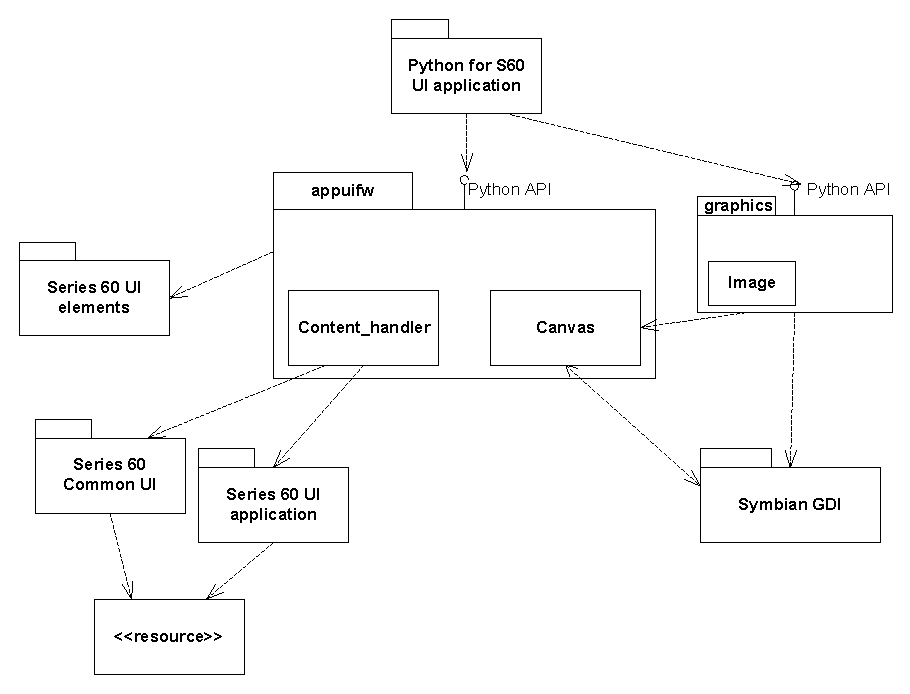
\includegraphics[width=\textwidth]{ui-overview}
\caption{Python for S60 UI environment overview}
\label{fig:ui-overview}
\end{figure}

\subsection{Basics of appuifw Module}
\label{subsec:basics}
Figure \ref{fig:normal-uilayout} shows the layout of a S60 application 
UI in the normal screen mode and a summary of how it relates to the services 
available at the \module{appuifw} API. For alternative layouts, see 
Figure \ref{fig:alternate-uilayouts}.

\begin{figure}
\centering
%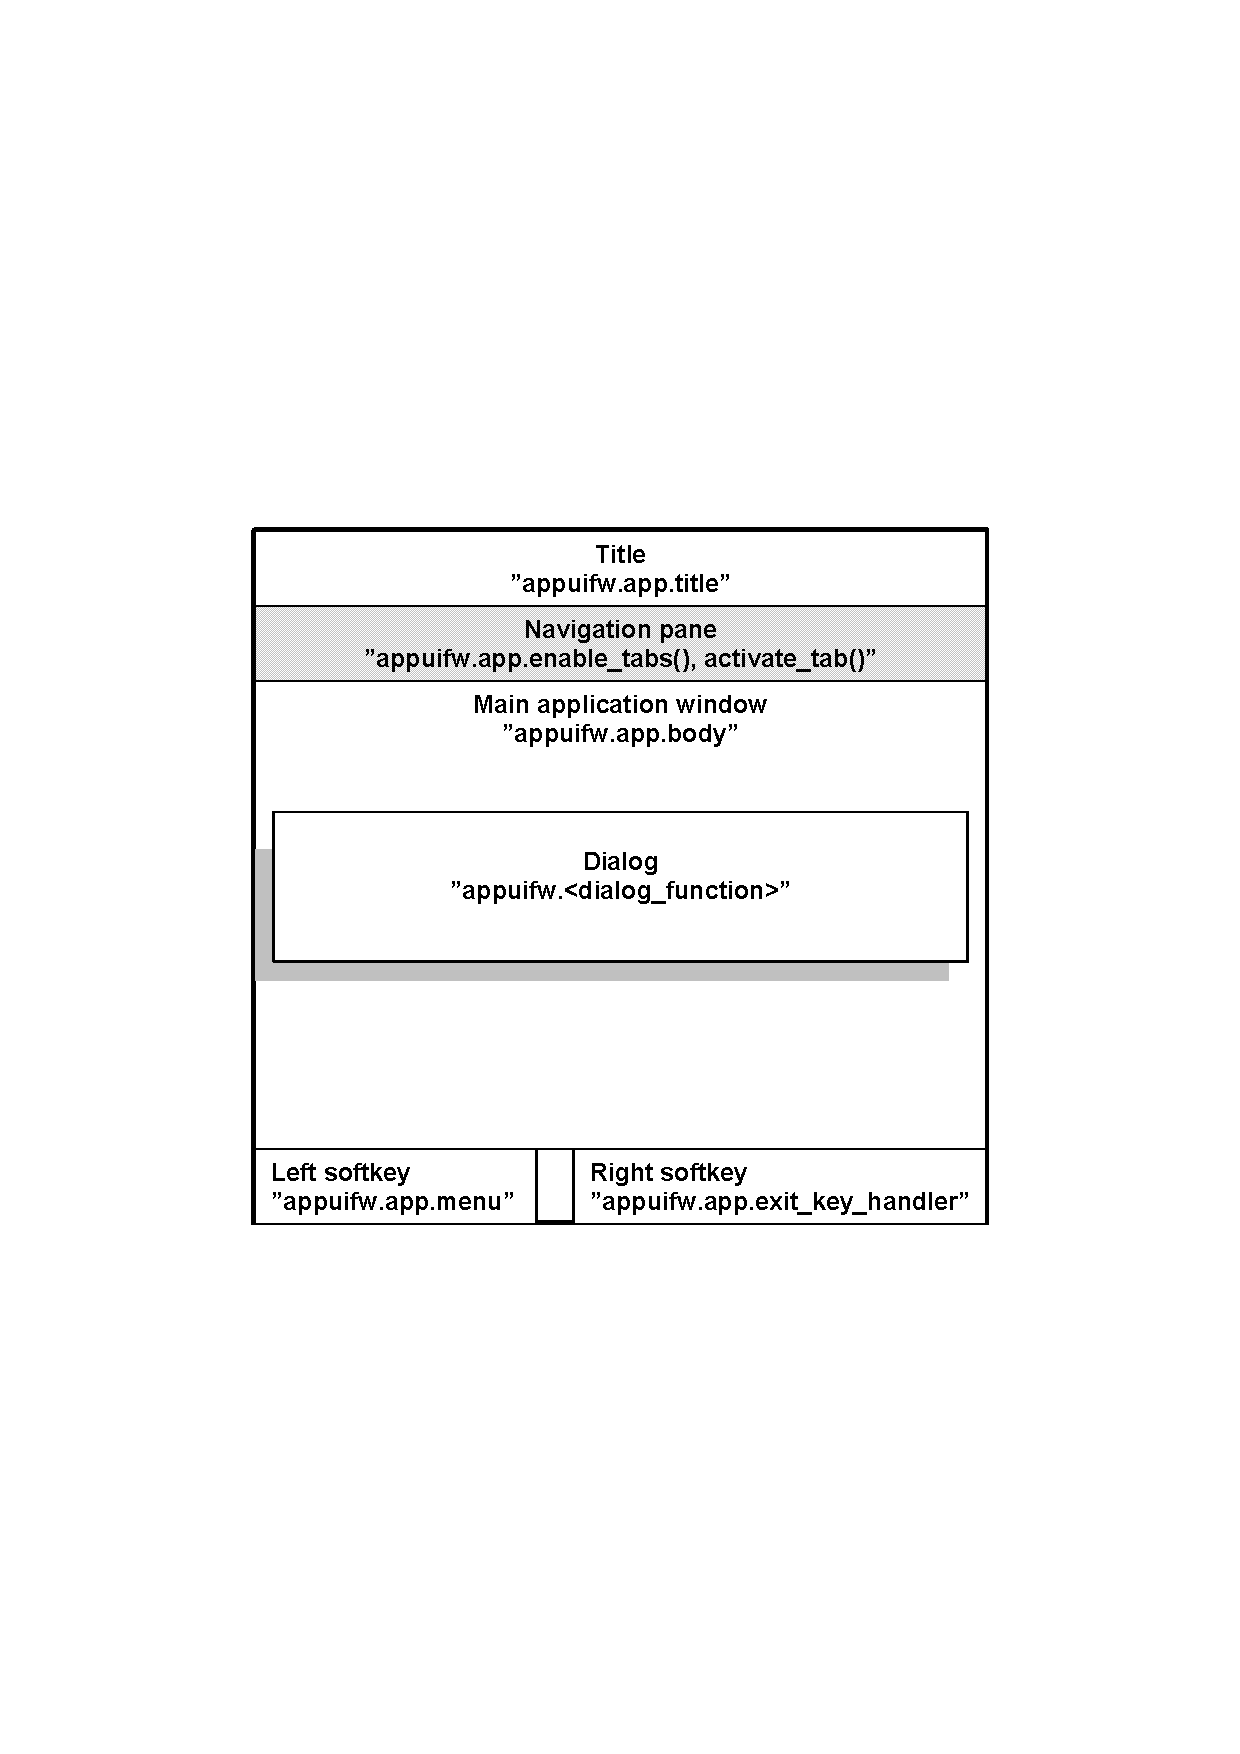
\includegraphics[width=0.7\textwidth]{screen-parts}
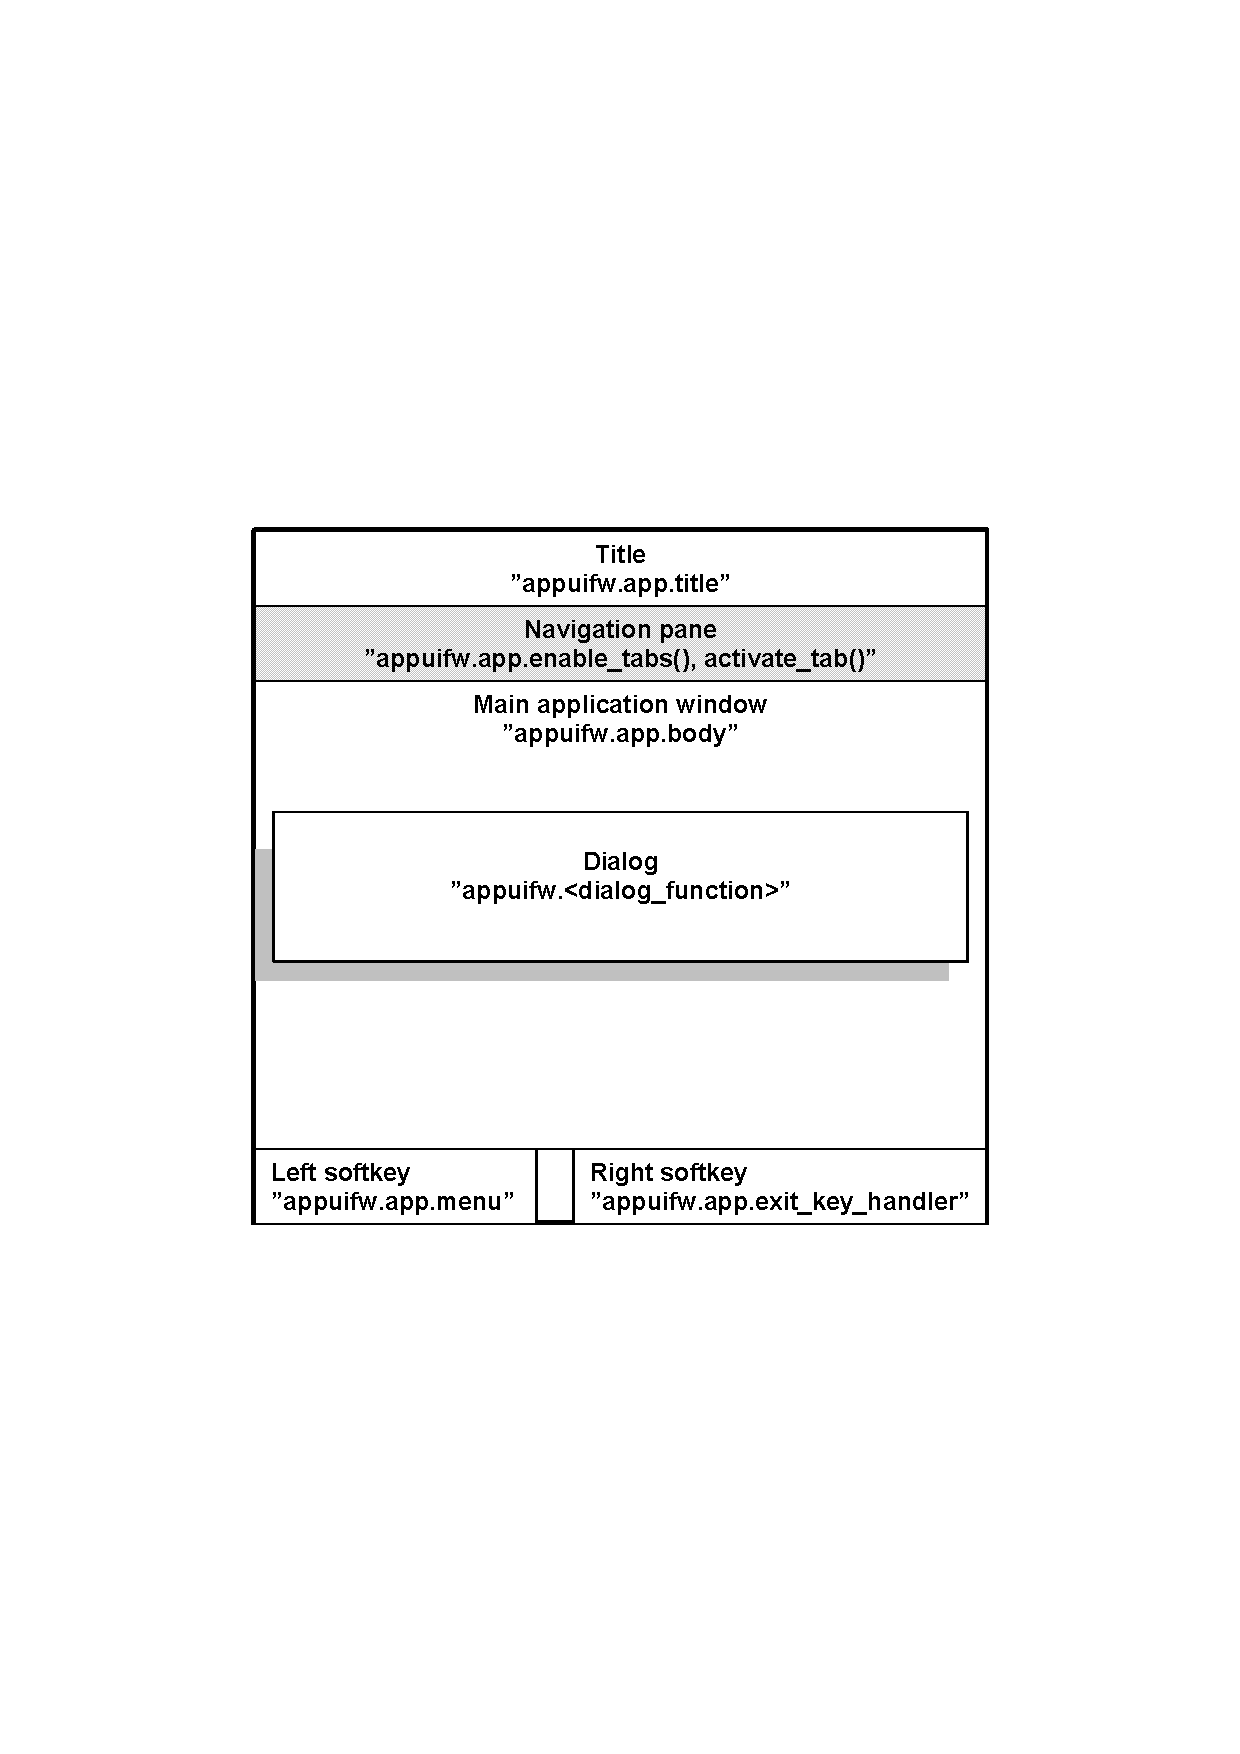
\includegraphics{screen-parts}
\caption{The different parts of the screen when using the 'normal' layout}
\label{fig:normal-uilayout}
\end{figure}

\begin{figure}
\centering
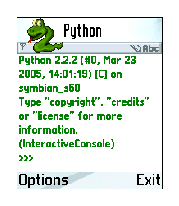
\includegraphics[width=\screenwidth]{layout-normal}
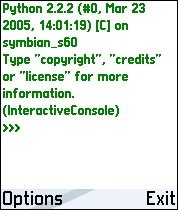
\includegraphics[width=\screenwidth]{layout-large}
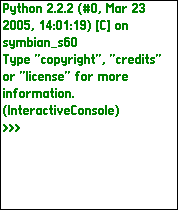
\includegraphics[width=\screenwidth]{layout-full}
\caption{UI layouts. left: 'normal', middle: 'large', right: 'full'}
\label{fig:alternate-uilayouts}
\end{figure}

The main application window may be set up to be occupied by a UI control.

A multi-view application can show the different views as tabs in the 
navigation pane and react as the users navigate between tabs. 

Dialogs always take precedence over the usual UI controls and appear on top 
of them.

UI controls are implemented as Python types. These types are available:

\begin{itemize}
\item \class{Text}
\item \class{Listbox}
\item \class{Canvas}
\end{itemize}
UI controls appear on the screen as soon as an instance of the corresponding 
Python type is set to the body field (\var{app.body}) of the current application UI.

\class{Form} is a versatile dialog implemented as a type.

The \class{Content_handler} type facilitates interfacing to other UI
applications and common high-level UI components. It is based on the
notion that designated handlers can reduce UI application interaction
to operations on MIME-type content.

The following dialogs are implemented as functions:

\begin{itemize}
\item \function{note}
\item \function{query}
\item \function{multi_query}
\item \function{selection_list}
\item \function{multi_selection_list}
\item \function{popup_menu}
\end{itemize}
A dialog becomes visible as soon as the corresponding Python function has 
been called. The function returns with the eventual user input or 
information on the cancellation of the dialog. \class{Form} is an 
exception; it is shown when its \method{execute} method is called.

\subsection{Softkeys}
\label{subsec:softkeys}
The softkeys are managed by the underlying S60 Platform. When no
dialog is visible, the right softkey is bound to application exit and
the left one represents an Options menu. Python for S60 offers
an interface for manipulating the menu and for binding the Exit key to
a Python-callable object (see Section \ref{subsec:application}). 

The native code that implements a dialog also manages the softkeys of the 
dialog, typically OK and Cancel. When the user input needs to be validated 
before accepting it and dismissing the dialog, it is best to use 
\class{Form}.

\subsection{Module Level Functions}
\label{subsec:module}
The following free functions - functions that do not belong to any class 
- are defined in the \module{appuifw} module:

\begin{funcdesc}{available_fonts}{}
Returns a list (Unicode) of all fonts available in the device.
\end{funcdesc}

\begin{funcdesc}{query}{label, type\optional{, initial_value}}
Performs a query with a single-field dialog. The prompt is set to 
\var{label}, and the type of the dialog is defined by \var{type}. The 
value of \var{type} can be any of the following strings:

\begin{itemize}
\item \code{'text'}
\item \code{'code'}
\item \code{'number'}
\item \code{'date'}
\item \code{'time'}
\item \code{'query'}
\item \code{'float'}
\end{itemize}

The type of the optional \var{initial_value} parameter and the 
returned input depend on the value of \var{type}:

\begin{itemize}
\item For text fields, (\code{'text'}, \code{'code'}) it is Unicode
\item For number fields, it is numeric
\item For date fields, it is seconds since epoch rounded down to the nearest local midnight
\end{itemize}

A simple confirmation query and time query take no initial value and return 
\code{True/None} and seconds since local midnight, correspondingly. All 
queries return \code{None} if the users cancel the dialog. 

For \code{'float'} query the \var{initial_value} setting has no 
effect.
\end{funcdesc}


\begin{funcdesc}{multi_query}{label_1, label_2}
A two-field text (Unicode) input dialog. Returns the inputted values
as a 2-tuple. Returns \code{None} if the users cancel the dialog.
\end{funcdesc}

\begin{funcdesc}{note}{text\optional{, type\optional{, global}}}
Displays a note dialog of the chosen type with \var{text} 
(Unicode). The default value for \var{type} is \code{'info'}, which is 
automatically used if \var{type} is not set. \var{type} can be one of 
the following strings: \code{'error'}, \code{'info'}, or 
\code{'conf'}. 

If \var{global} (integer) is any other value than zero a global note is 
displayed. A global note is displayed even if the Python application calling 
this function is in background. The same set of \var{type}s is supported as in 
standard note.
\end{funcdesc}

\begin{funcdesc}{popup_menu}{list\optional{, label}}
A pop-up menu style dialog. \var{list} representing the menu 
contents can be a list of Unicode strings or a list of Unicode string pairs 
(tuples). The resulting dialog list is then a single-style or a double-style 
list. A single-style list is shown in full; whereas a double-style list 
shows the items one at a time. Returns \code{None} if the user cancels the 
operation.
\end{funcdesc}

\begin{funcdesc}{selection_list}{choices\optional{, search_field=0}}
Executes a dialog that allows the users to select a list item and
returns the \var{index} of the chosen item, or \code{None} if the
selection is cancelled by the users. \var{choices} is a list of
Unicode strings.
\var{search_field} is \code{0} (disabled) by default and is optional. Setting it to \code{1} enables a search field (find pane) that facilitates searching for items in long lists. If enabled, the search field appears after you press a letter key.
\end{funcdesc}

\begin{funcdesc}{multi_selection_list}{choices\optional{, style='checkbox', search_field=0}}
  Executes a dialog that allows the users to select multiple list
  items.  Returns a tuple of indexes (a pair of Unicode strings) of
  the chosen items, or empty tuple if the selection is cancelled by
  the users. \var{choices} is a list of Unicode strings.  \var{style}
  is an optional string; the default value being \code{'checkbox'}.
  If \code{'checkbox'} is given, the list will be a checkbox list,
  where empty checkboxes indicate what items can be marked. The other
  possible value that can be set for \var{style} is
  \code{'checkmark'}. If \code{'checkmark'} is given, the list will be
  a markable list, which lists items but does not indicate
  specifically that items can be selected. To select items on a
  markable list, use the Navigation key to browse the list and the
  Edit key to select an item. For example views on checkbox and
  markable lists, see
  \figurename~\ref{fig:checkbox-and-markable-list}.
  \var{search_field} is \code{0} (disabled) by default and is
  optional. Setting it to \code{1} enables a search field (find pane)
  that facilitates searching for items in long lists. If enabled, the
  search field is always visible with checkbox lists; with markable
  lists it appears by pressing a letter key.

Example:
\begin{verbatim}
tuple = appuifw.multi_selection_list(L, style='checkmark', search_field=1)
\end{verbatim}
\end{funcdesc}

\begin{figure}[htbp]
\centering
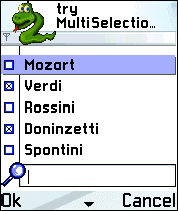
\includegraphics[width=\screenwidth]{checkbox-list}
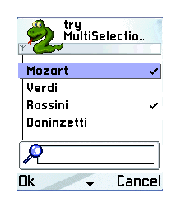
\includegraphics[width=\screenwidth]{markable-list}
\caption{Examples of a checkbox list (left) and a markable list (right)}
\label{fig:checkbox-and-markable-list}
\end{figure}

\subsection{Application Type}
\label{subsec:application}
A single implicit instance of this type always exists when \module{appuifw} 
module is present and can be referred to with the name \code{app}. New 
instances cannot be created by a Python program.

\begin{classdesc*}{Application}
Instances of \class{Application} type have the following attributes:

\begin{memberdesc}[Application]{body}
The UI control that is visible in the application's main window. Currently 
either \class{Text}, a \class{Listbox} object, \class{Canvas}, or 
\code{None}.
\end{memberdesc}

\begin{memberdesc}[Application]{exit_key_handler}
A callable object that is called when the user presses the Exit softkey. 
Setting \member{exit_key_handler} to \code{None} sets it back to the 
default value.
\end{memberdesc}

\begin{memberdesc}[Application]{menu}
This is a list of the following kinds of items:
\begin{itemize}
\item \code{(title, callback)} which creates a regular menu item
\item \code{(title, ((title, callback)\optional{...}))} which creates a submenu
\end{itemize}

\var{title} (Unicode) is the name of the item and \var{callback} the associated callable object. 
The maximum allowed number of items in a menu, or items in a submenu,
or submenus in a menu is 30.

Example:
\begin{verbatim}
appuifw.app.menu = [(u"Item 1", item1),
                    (u"Submenu 1", 
                        ((u"Subitem 1", subitem1),
                         (u"Subitem 2", subitem2)))]
\end{verbatim}
\end{memberdesc}

\begin{memberdesc}[Application]{screen}
The screen area used by an application. See \figurename~\ref{fig:alternate-uilayouts} for
example screens. The appearance of the application on the screen can
be affected by setting one of the following values: \code{'normal'},
\code{'large'}, and \code{'full'}.

Examples:
\begin{verbatim}
appuifw.app.screen='normal' # (a normal screen with title pane and softkeys)
appuifw.app.screen='large'  # (only softkeys visible)
appuifw.app.screen='full'   # (a full screen)
\end{verbatim}
\end{memberdesc}

\begin{memberdesc}[Application]{title}
The title the application that is visible in the application's title
pane. Must be Unicode.
\end{memberdesc}

\begin{memberdesc}[Application]{focus}
A callable object that is called with integer as parameter (0 = focus lost, 
1 = focus regained) when the application receives focus or it is switched to 
background. Focus is received e.g. when the application is switched from 
background to foreground or when the focus is regained from screensaver. 
Similarly when the screensaver is displayed, focus is lost.

Examples:
\begin{verbatim}
>>> import appuifw
>>> def cb(fg):
...   if(fg):
...     print "foreground"
...   else:
...     print "background"
...
>>> appuifw.app.focus=cb
>>> # switch to background, following text is printed from callback:
>>> background
>>> # switch to foreground, following text is printed from callback:
>>> foreground
\end{verbatim}

\begin{notice}
An improper callback can cause adverse effects. If you, for example,
define a callback which takes no parameters you will receive
never-ending \exception{TypeError} exceptions on the Nokia 6600.
\end{notice}

\end{memberdesc}

\begin{memberdesc}[Application]{orientation}
Available only for S60 3rdEd. 
The orientation of the application. The orientation of the application can be 
one of the following values: \code{'automatic'} (this is the default value), 
\code{'portrait'} or \code{'landscape'}.
\end{memberdesc}

Instances of \class{Application} type have the following methods:

\begin{methoddesc}[Application]{activate_tab}{index}
Activates the tab \var{index} counting from zero.
\end{methoddesc}

\begin{methoddesc}[Application]{full_name}{}
Returns the full name, in Unicode, of the native application in whose 
context the current Python interpreter session runs.
\end{methoddesc}

\begin{methoddesc}[Application]{uid}{}
Returns the UID, in Unicode, of the native application in whose 
context the current Python interpreter session runs.
\end{methoddesc}

\begin{methoddesc}[Application]{set_exit}{}
Requests a graceful exit from the application as soon as the current script 
execution returns.
\end{methoddesc}

\begin{methoddesc}[Application]{set_tabs}{tab_texts\optional{,callback=None}}
Sets tabs with given names on them in the navigation bar; 
\var{tab_texts} is a list of Unicode strings. When the users 
navigate between tabs, \var{callback} gets called with the index 
of the active tab as an argument. Tabs can be disabled by giving an empty or 
one-item \var{tab_texts} list.
\end{methoddesc}


\begin{methoddesc}[Application]{layout}{layout_id}

\begin{notice}[note]
Available from S60 2ndEd FP3 onwards (inclusive).
\end{notice}

Returns as a tuple the size and the position of the requested \code{layout_id}. 
The logical layouts are outlined partly in Figure \ref{fig:normal-uilayout}. The 
position is given from the top left corner. The \code{layout_id} can be one of 
the constants defined in module \module{appuifw}\footnote{Descriptions of the 
values are from the S60 SDK documentation \cite{S60Doc}.}:

\begin{datadesc}{EScreen} 
Screen.  
\end{datadesc}

\begin{datadesc}{EApplicationWindow} 
 Window that fills the entire screen.
\end{datadesc}

\begin{datadesc}{EStatusPane} 
Indicates common components for most of the applications.  
\end{datadesc}

\begin{datadesc}{EMainPane} 
The application main pane is used in all the applications.  
\end{datadesc}

\begin{datadesc}{EControlPane} 
Control pane.
\end{datadesc}

\begin{datadesc}{ESignalPane} 
The signal pane is used to indicate signal strength.  
\end{datadesc}

\begin{datadesc}{EContextPane} 
The context pane is used to indicate an active application.
\end{datadesc}

\begin{datadesc}{ETitlePane} 
Used to indicate the subject or the name of the main pane content. 
\end{datadesc}

\begin{datadesc}{EBatteryPane} 
The battery pane is used to indicate battery strength.  
\end{datadesc}

\begin{datadesc}{EUniversalIndicatorPane} 
The universal indicator pane is used to indicate items that require the user's 
attention while browsing applications. 
\end{datadesc}

\begin{datadesc}{ENaviPane} 
The navi pane is used to indicate navigation within an application, to provide 
context sensitive information to the user while entering or editing data, or to 
show additional information.  
\end{datadesc}

\begin{datadesc}{EFindPane} 
A fixed find pane is used with lists instead of the find pop-up window.  
\end{datadesc}

\begin{datadesc}{EWallpaperPane} 
Wallpaper pane.  
\end{datadesc}

\begin{datadesc}{EIndicatorPane} 
The universal indicator pane is used to indicate items that require the user's 
attention while browsing applications.  
\end{datadesc}

\begin{datadesc}{EAColumn} 
Used generally to display small sized graphics or heading texts.  
\end{datadesc}

\begin{datadesc}{EBColumn} 
Used generally to display large sized icons or heading texts.  
\end{datadesc}

\begin{datadesc}{ECColumn} 
Used generally to display data entered by the user. Overlaps with the D column. 
\end{datadesc}

\begin{datadesc}{EDColumn} 
Used generally to display additional icons. Overlaps with the C column. 
\end{datadesc}

\begin{datadesc}{EStaconTop} 
Top part of status and control panes in landscape layout.  
\end{datadesc}

\begin{datadesc}{EStaconBottom} 
Bottom part of status and control panes in landscape layout.  
\end{datadesc}

\begin{datadesc}{EStatusPaneBottom} 
Bottom part of status pane in landscape layout.  
\end{datadesc}

\begin{datadesc}{EControlPaneBottom} 
Bottom part of control pane in landscape layout.  
\end{datadesc}

\begin{datadesc}{EControlPaneTop} 
Top part of control pane in landscape layout.  
\end{datadesc}

\begin{datadesc}{EStatusPaneTop} 
Top part of status pane in landscape layout.
\end{datadesc}

Example:
\begin{verbatim}
>>> import appuifw
>>> appuifw.app.layout(appuifw.EMainPane)
((176, 144), (0, 44))
>>> # size and position (x, y) of the main pane in Nokia N70
\end{verbatim}

\end{methoddesc}

\end{classdesc*}

\subsection{Form Type}
\label{subsec:form}
\class{Form} implements a dynamically configurable, editable multi-field 
dialog. \class{Form} caters for advanced dialog use cases with requirements 
such as free selectability of the combination of fields, possibility of 
validating the user input, and automatically producing the contents of some 
dialog fields before allowing the closing of the dialog. 

\begin{classdesc}{Form}{fields\optional{, flags=0}}
Creates a \class{Form} instance.
\var{fields} is a list of \emph{field descriptors}: \code{(label, type\optional{, value})} where

\var{label} is a Unicode string

\var{type} is one of the following strings: 
\code{'text'}, \code{'number'}, \code{'date'}, \code{'time'}, \code{'combo'}
or \code{'float'}

\var{value}, depending on \var{type}: Unicode string, numeric, float (seconds 
since Unix epoch rounded down to the nearest local midnight), float (seconds 
since local midnight), \code{([choice_label ...], index)} of float. For 
\code{'float'} \var{type} the initial value setting might not be shown in the 
UI.
\end{classdesc}

\class{Form} can also be configured and populated after construction. The 
configuration flags are visible as an attribute. \class{Form} implements 
the list protocol that can be used for setting the form fields, as well as 
obtaining their values after the dialog has been executed.

Instances of \class{Form} type have the following attributes:

\begin{memberdesc}[Form]{flags}
This attribute holds the values of the various configuration flags. 
Currently supported flags are:

\begin{datadesc}{FFormEditModeOnly}
When this flag is set, the form remains in edit mode while \method{execute} 
runs.
\end{datadesc}

\begin{datadesc}{FFormViewModeOnly}
When this flag is set, the form cannot be edited at all.
\end{datadesc}

\begin{datadesc}{FFormAutoLabelEdit}
This flag enables support for allowing the end-users to edit the labels of 
the form fields.
\end{datadesc}

\begin{datadesc}{FFormAutoFormEdit}
This flag enables automatic support for allowing the end-users to add and 
delete the form fields. Note that this is an experimental feature and is not 
guaranteed to work with all SDK versions.
\end{datadesc}

\begin{datadesc}{FFormDoubleSpaced}
When this flag is set, double-spaced layout is applied when the form is 
executed: one field takes two lines, as the label and the value field are on 
different lines.
\end{datadesc}
\end{memberdesc}

\begin{memberdesc}[Form]{menu}
A list of \code{(title, callback)} pairs, where 
each pair describes an item in the form's menu bar that is active while the 
dialog is being executed. \var{title} (Unicode) is the name of 
the item and \var{callback} the associated callable object.
\end{memberdesc}

\begin{memberdesc}[Form]{save_hook}
This attribute can be set to a callable object that receives one argument 
and returns a Boolean value. It gets called every time the users want to 
save the contents of an executing \class{Form} dialog. A candidate list for 
new form content - a list representing the currently visible state of the 
UI - is given as an argument. The list can be modified by 
\member{save_hook}. If \member{save_hook} returns \code{True}, the 
candidate list is set as the new contents of the form. Otherwise, the form 
UI is reset to reflect the field list contained in \class{Form} object.
\end{memberdesc}

Instances of \class{Form} type have the following methods:

\begin{methoddesc}[Form]{execute}{}
Executes the dialog by making it visible on the UI.
\end{methoddesc}

\begin{methoddesc}[Form]{insert}{index, field_descriptor}
Inserts the field descriptor into the \class{Form} before the given \var{index}.
\end{methoddesc}

\begin{methoddesc}[Form]{pop}{}
Removes the last field descriptor from the \class{Form} and returns it.
\end{methoddesc}

\begin{methoddesc}[Form]{length}{}the number of field descriptors in the form.
\end{methoddesc}

The subscript notation \code{f[i]} can be used to access or modify the
i-th element of the form \code{f}. Same limitations as discussed above
in the context of the flag \constant{FFormAutoFormEdit} apply to
modifying a form while it is executing. The ability to change the
schema of a form while it is executing is an experimental feature.

\subsection{Text Type}
\label{subsec:mylabel5}
\class{Text} is a text editor UI control. For examples on the options 
available with \class{Text}, see Figure \ref{fig:text-styles}.

\begin{figure}[htbp]
\centering
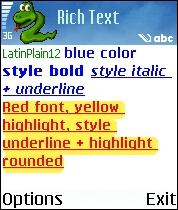
\includegraphics[width=\screenwidth]{text-styles-1}
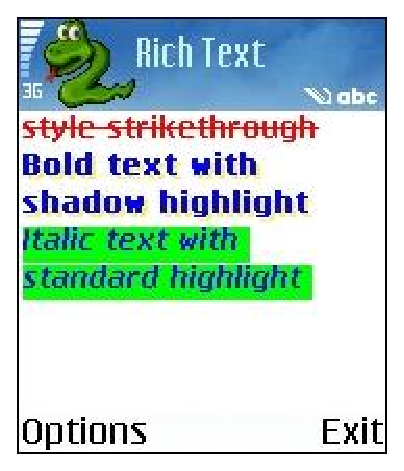
\includegraphics[width=\screenwidth]{text-styles-2}
\caption{Examples of the options available for Text type}
\label{fig:text-styles}
\end{figure}

Instances of \class{Text} type have the following attributes:

\begin{memberdesc}[Text]{color}
The color of the text. \code{color} supports the same color representation 
models as the \module{graphics} module. For the supported color 
representation models, see Section \ref{sec:graphics}.
\end{memberdesc}

\begin{memberdesc}[Text]{focus}
A Boolean attribute that indicates the focus state of the control. Editor 
control also takes the ownership of the navigation bar, and this feature is 
needed to enable the usage of this control in applications that use the 
navigation bar - for example, navigation tabs.
\end{memberdesc}

\begin{memberdesc}[Text]{font} 
The font of the text. There are two possible ways to set this attribute:

\begin{itemize}

\item Using a supported Unicode font, for example \code{u"Latin12"}. Trying to set a font which is not supported by the device has no effect. A list of supported fonts can be retrieved by using \function{appuifw.available_fonts}.

Example, setting font:
\begin{verbatim}
t = appuifw.Text()
t.font = u"albi17b" # sets font to Albi 17 bold
t.font = u"LatinPlain12" # sets font to Latin Plain 12
\end{verbatim}
\item Using one of the default device fonts that are associated with the following labels (plain strings):
\code{'annotation', 'title', 'legend', 'symbol', 'dense', 'normal'}
Example, setting font: 
\begin{verbatim}
t.font = "title" # sets font to the one used in titles
\end{verbatim}

Example, checking the currently set font: 
\begin{verbatim}
unicodeFont = t.font
\end{verbatim}
\end{itemize}

The attribute value retrieved is always a Unicode string. If the font has 
been set with a label, for example, \code{'title'}, the attribute will 
retrieve the font associated with that label. 
\end{memberdesc}

\begin{memberdesc}[Text]{highlight_color}
The highlight color of the text. \code{highlight_color} supports the 
same color representation models as the \module{graphics} module. For the 
supported color representation models, see Section \ref{sec:graphics}.
\end{memberdesc}

\begin{memberdesc}[Text]{style}
The style of the text. The flags for this attribute are defined in the 
\module{appuifw} module. These flags can be combined by using the binary 
operator \code{|}. The flags can be divided into two types: text style 
and text highlight. Text style flags can be freely combined with each other. 
However, one or more text style flags can be combined with only one text 
highlight flag. The flags are:

Text style:

\begin{datadesc}{STYLE_BOLD} 
Enables bold text.
\end{datadesc}

\begin{datadesc}{STYLE_UNDERLINE}
Enables underlined text.
\end{datadesc}

\begin{datadesc}{STYLE_ITALIC} 
Enables italic text.
\end{datadesc}

\begin{datadesc}{STYLE_STRIKETHROUGH } 
Enables strikethrough.
\end{datadesc}

Text highlight:

\begin{datadesc}{HIGHLIGHT_STANDARD}
Enables standard highlight.
\end{datadesc}

\begin{datadesc}{HIGHLIGHT_ROUNDED}
Enables rounded highlight.
\end{datadesc}

\begin{datadesc}{HIGHLIGHT_SHADOW}
Enables shadow highlight.
\end{datadesc}

Only one highlight is allowed to be used at once. Therefore, it is possible 
to combine only one highlight with one or more text styles.

Examples:
\begin{verbatim}
t = appuifw.Text()

# These and other similar values and combinations are valid:
t.style = appuifw.STYLE_BOLD
t.style = appuifw.STYLE_UNDERLINE
t.style = appuifw.STYLE_ITALIC
t.style = appuifw.STYLE_STRIKETHROUGH
t.style = (appuifw.STYLE_BOLD|
	   appuifw.STYLE_ITALIC|
	   appuifw.STYLE_UNDERLINE)

# These values are valid:
t.style = appuifw.HIGHLIGHT_STANDARD
t.style = appuifw.HIGHLIGHT_ROUNDED
t.style = appuifw.HIGHLIGHT_SHADOW

# This combination is NOT valid:
# Invalid code, do not try!
t.style = (appuifw.HIGHLIGHT_SHADOW|appuifw.HIGHLIGHT_ROUNDED)
\end{verbatim}
\end{memberdesc}

Instances of \class{Text} type have the following methods:

\begin{methoddesc}[Text]{add}{text}
Inserts the Unicode string \var{text} to the current cursor position.
\end{methoddesc}

\begin{methoddesc}[Text]{bind}{event_code, callback}
Binds the callable Python object \var{callback} to event
\var{event_code}. The key codes are defined in 
the \module{key_codes} library module. The call 
\code{bind(event_code, None)} clears an 
existing binding. In the current implementation the event is always
passed also to the underlying native UI control.
\end{methoddesc}

\begin{methoddesc}[Text]{clear}{}
Clears the editor.
\end{methoddesc}

\begin{methoddesc}[Text]{delete}{\optional{pos=0, length=len()}}
Deletes \var{length} characters of the text held by the editor control, 
starting from the position \var{pos}.
\end{methoddesc}

\begin{methoddesc}[Text]{get_pos}{}
Returns the current cursor position.
\end{methoddesc}

\begin{methoddesc}[Text]{len}{}
Returns the length of the text string held by the editor control.
\end{methoddesc}

\begin{methoddesc}[Text]{get}{\optional{pos=0, length=len()}}
Retrieves \code{length} characters of the text held by the editor control, 
starting from the position \var{pos}.
\end{methoddesc}

\begin{methoddesc}[Text]{set}{text}
Sets the text content of the editor control to Unicode string 
\var{text}.
\end{methoddesc}

\begin{methoddesc}[Text]{set_pos}{cursor_pos}
Sets the cursor to \var{cursor_pos}.
\end{methoddesc}

\subsection{Listbox Type}
\label{subsec:listbox}

\begin{figure}[htbp]
\centering
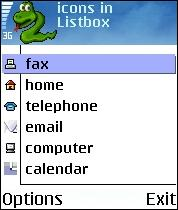
\includegraphics[width=\screenwidth]{listbox-with-icons}
\caption{Listbox with icons}
\label{fig:listbox-with-icons}
\end{figure}

An instance of this UI control type is visible as a listbox, also known as a 
list in Symbian, that can be configured to be a single-line item or a 
double-item listbox. Figure \ref{fig:listbox-with-icons} shows a single-line 
item Listbox with icons. For more information on the MBM and MIF formats, 
see Section \ref{subsec:icon}.

\begin{classdesc}{Listbox}{list, callback}
Creates a \class{Listbox} instance. A callable object 
\var{callback} gets called when a listbox selection has been 
made. \code{list} defines the content of the listbox and can be one of the 
following:

\begin{itemize}
\item A normal (single-line item) listbox: a list of Unicode strings, for example \code{[unicode_string item1, unicode_string item2]}
\item A double-item listbox: a two-element tuple of Unicode strings , for example \code{[(unicode_string item1, unicode_string item1description), (unicode_string item2, unicode_string item2description)]}
\item A normal (single-line item) listbox with graphics: a two-element tuple consisting of a Unicode string and an \class{Icon} object, for example \code{[(unicode_string item1, icon1), (unicode_string item2, icon2)]}.
\item A double-item listbox with graphics: a three-element tuple consisting of two Unicode strings and one \class{Icon} object, for example \code{[(unicode_string item1, unicode_string item1description, icon1), (unicode_string item2, unicode_string item2description, icon2)]}
\end{itemize}

Example: To produce a normal (single-line item) listbox with graphics:
\begin{verbatim}
icon1 = appuifw.Icon(u"z:\\system\\data\\avkon.mbm", 28, 29)
icon2 = appuifw.Icon(u"z:\\system\\data\\avkon.mbm", 40, 41)
entries = [(u"Signal", icon1),
           (u"Battery", icon2)]
lb = appuifw.Listbox(entries, lbox_observe)
\end{verbatim}
\end{classdesc}

Instances of \class{Listbox} type have the following methods:

\begin{methoddesc}[Listbox]{bind}{event_code, callback}
Binds the callable Python object \var{callback} to event 
\var{event_code}. The key codes are defined in 
the \module{key_codes} library module. The call
\code{bind(event_code, None)} clears an 
existing binding. In the current implementation the event is always passed 
also to the underlying native UI control.
\end{methoddesc}

\begin{methoddesc}[Listbox]{current}{}
Returns the currently selected item's index in the \class{Listbox}.
\end{methoddesc}

\begin{methoddesc}[Listbox]{set_list}{list\optional{, current}}
Sets the \class{Listbox} content to a list of Unicode strings or a
list of tuples of Unicode strings. The accepted structures of \var{list} are the
same as in the \class{Listbox} constructor. The optional argument \var{current} is the index of the focused list item.
\end{methoddesc}

\subsection{Icon Type}
\label{subsec:icon}
An instance of \class{Icon} type encapsulates an icon to be used together 
with a \class{Listbox} instance. Note that currently \class{Icon} can only 
be used with \class{Listbox} (see Section \ref{subsec:listbox}).

MBM is the native Symbian OS format used for pictures. It is a
compressed file format where the files can contain several bitmaps and
can be referred to by a number. An \code{.mbg} file is the header file
usually associated with an \code{.mbm} file, which includes symbolic
definitions for each bitmap in the file. For example, an
\file{avkon.mbm} file has an associated index file called
\file{avkon.mbg}, which is included in S60 SDKs. For more information
on the MBM format and the bitmap converter tool, see \cite{S60Doc} and
search the topics with the key term "How to provide Icons"; this topic
also points you to the Bitmap Converter tool that can be used for
converting bitmaps into the MBM format.

S60 2$^{nd}$ Edition FP3 introduces a new format for icons called 
Multi-Image File (MIF). This format is very similar to the MBM format and 
also contains several compressed files. The files to be compressed should be 
in Scalable Vector Graphics Tiny (SVG-T) format. For more information on the 
SVG format, see Scalable Vector Graphics (SVG) 1.1 Specification 
[10].

\begin{classdesc}{Icon}{filename, bitmap, bitmapMask}
Creates an icon. \var{filename} is a Unicode file name and must 
include the whole path. Note that MBM and MIF (MIF only in S60 2nd 
Edition FP3) are the only file formats supported. \var{bitmap} 
and \var{bitmapMask} are integers that represent the index of 
the icon and icon mask inside that file respectively.
\end{classdesc}

Example: The following builds an icon with the standard signal symbol:
\begin{verbatim}
icon = appuifw.Icon(u"z:\\system\\data\\avkon.mbm", 28, 29)
\end{verbatim}

\subsection{Content_handler Type}
\label{subsec:content}

An instance of \class{Content_handler} handles data content by its MIME 
type.

\begin{classdesc}{Content_handler}{\optional{callback}}
Creates a \class{Content_handler} instance. A Content_handler handles
data content by its MIME type. The optional
\var{callback} is called when the embedded handler application 
started with the \method{open} method finishes. 
\end{classdesc}

Instances of \class{Content_handler} type have the following methods:

\begin{methoddesc}[Content_handler]{open}{filename}
Opens the file \var{filename} (Unicode) in its handler 
application if one has been registered for the particular MIME type. The 
handler application is embedded in the caller's thread. The call to this 
function returns immediately. When the handler application finishes, the 
\var{callback} that was given to the \class{Content_handler} 
constructor is called.
\end{methoddesc}

\begin{methoddesc}[Content_handler]{open_standalone}{filename}
Opens the file \var{filename} (Unicode) in its handler 
application if one has been registered for the particular MIME type. The 
handler application is started in its own process. The call to this function 
returns immediately. Note that \var{callback} is not called for 
applications started with this method.
\end{methoddesc}

\subsection{Canvas Type}
\label{subsec:canvas}
\class{Canvas} is a UI control that provides a drawable area on the screen 
and support for handling raw key events. \class{Canvas} supports the 
standard drawing methods that are documented in Section \ref{sec:graphics}.

\begin{classdesc}{Canvas}{\optional{redraw_callback=None, event_callback=None,
                                  resize_callback=None}}
Constructs a \class{Canvas}. The optional parameters are callbacks
that are called when specific events occur. 

\note{Watch out for cyclic
references here. For example, if the callbacks are methods of an
object that holds a reference to the \class{Canvas}, a reference cycle
is formed that must be broken at cleanup time or the
\class{Canvas} will not be freed.}

\var{redraw_callback} is called whenever a part of the \class{Canvas} 
has been obscured by something, is then revealed, and needs to be
redrawn. This can typically happen, for example, when the user
switches away from the Python application and back again, or after
displaying a pop-up menu. The callback takes as its argument a
four-element tuple that contains the top-left and the bottom-right
corner of the area that needs to be redrawn. In many cases redrawing
the whole
\class{Canvas} is a reasonable option. 

\var{event_callback} is called whenever a raw key event is received.
There are three kinds of key events: \code{EEventKeyDown},
\code{EEventKey}, and \code{EEventKeyUp}. When a user presses a key 
down, events \code{EEventKeyDown} and \code{EEventKey} are generated. 
When the key is released, an \code{EEventKeyUp} event is generated.

The argument to the \var{event_callback} is a dictionary that contains 
the following data for key events:

\begin{itemize}
\item \code{'type'}: one of \code{EEventKeyDown}, \code{EEventKey}, or \code{EEventKeyUp}
\item \code{'keycode'}: the keycode of the key
\item \code{'scancode'}: the scancode of the key
\item \code{'modifiers'}: the modifiers that apply to this key event
\end{itemize}

Each key on the keyboard has one or more scancodes and zero or more keycodes 
associated with it. A scancode represents the physical key itself and a 
keycode is the result of state-related operating system defined processing 
done on the key. For keys that correspond to a symbol in the current 
character set of the phone, the keycode is equal to the code of the 
corresponding symbol in that character set. For example, if you are using 
the Nokia Wireless Keyboard (SU-8W), pressing the key A will always produce 
the scancode 65 (ASCII code for an upper case A), but the keycode 
could be either 65 or 91 (ASCII code for a lower case A) depending on 
whether or not the Shift key is pressed or Caps Lock is active. 

The \module{key_codes} module contains definitions for the keycodes and 
scancodes. See \figurename~\ref{fig:keyboard} for the codes of the most 
common keys on the phone keypad. 

Some keys are handled in a special way:

\begin{itemize}
\item A short press of the Edit key causes it to stay down, meaning that no \code{EEventKeyUp} event is sent. The event is only sent after a long press.
\item Detecting presses of the Voice tags key or the Power key is not supported.
\item If the right softkey is pressed, the \code{appuifw.app.exit_key_handler} callback is always executed.
\end{itemize}

There is no way to prevent the standard action of the Hang-up key, the Menu 
key, the Power key or the Voice tags key from taking place.

\begin{figure}
\centering
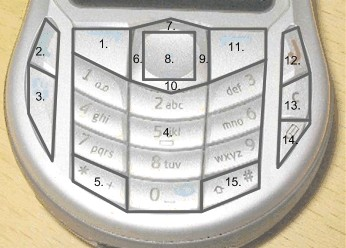
\includegraphics[width=5in]{6630keyboard}
%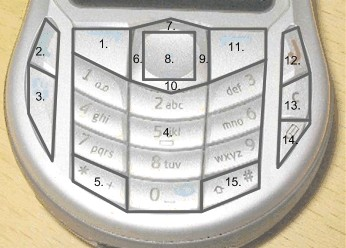
\includegraphics[width=3.60in,height=2.58in]{6630keyboard}
%\centerline{\includegraphics[width=3.60in,height=2.58in]{API_Reference_for_Python11.eps}} \par & 
\begin{tableiii}{lll}{textrm}{Key}{Keycode}{Scancode}
\lineiii{1.}{EKeyLeftSoftkey}{EScancodeLeftSoftkey}
\lineiii{2.}{EKeyYes}{EScancodeYes}
\lineiii{3.}{EKeyMenu}{EScancodeMenu}
\lineiii{4.}{EKey0...9}{EScancode0...9}
\lineiii{5.}{EKeyStar}{EScancodeStar}
\lineiii{6.}{EKeyLeftArrow}{EScancodeLeftArrow}
\lineiii{7.}{EKeyUpArrow}{EScancodeUpArrow}
\lineiii{8.}{EKeySelect}{EScancodeSelect}
\lineiii{9.}{EKeyRightArrow}{EScancodeRightArrow}
\lineiii{10.}{EKeyDownArrow}{EScancodeDownArrow}
\lineiii{11.}{EKeyRightSoftkey}{EScancodeRightSoftkey}
\lineiii{12.}{EKeyNo}{EScancodeNo}
\lineiii{13.}{EKeyBackspace}{EScancodeBackspace}
\lineiii{14.}{EKeyEdit}{EScancodeEdit}
\lineiii{15.}{EKeyHash}{EScancodeHash}
\end{tableiii}
\caption{Keycodes and scancodes for phone keys usable from Python applications}
\label{fig:keyboard}
\end{figure}

\var{resize_callback} is called when screen size is changed when the 
\class{Canvas} rect size has been changed. The callback takes as its argument a
two-element tuple that contains the new clientRect width and height. 

\end{classdesc}

Instances of \class{Canvas} type have the following attribute:

\begin{memberdesc}[Canvas]{size}
A two-element tuple that contains the current width and height of the 
\class{Canvas} as integers.
\end{memberdesc}

Instances of \class{Canvas} type have the same standard drawing methods 
that are documented in Section \ref{sec:graphics}.

% Copyright (c) 2005-2007 Nokia Corporation
%
% Licensed under the Apache License, Version 2.0 (the "License");
% you may not use this file except in compliance with the License.
% You may obtain a copy of the License at
%
%     http://www.apache.org/licenses/LICENSE-2.0
%
% Unless required by applicable law or agreed to in writing, software
% distributed under the License is distributed on an "AS IS" BASIS,
% WITHOUT WARRANTIES OR CONDITIONS OF ANY KIND, either express or implied.
% See the License for the specific language governing permissions and
% limitations under the License.

\newcommand{\notinfirsted}{
\begin{notice}
Not supported in S60 1st Edition!
\end{notice}

}

\section{\module{graphics} ---
  A graphics related services package}
\label{sec:graphics}

\declaremodule{extension}{graphics}
\platform{S60}
\modulesynopsis{A graphics related services package.}

The \module{graphics} module provides access to the graphics primitives and 
image loading, saving, resizing, and transformation capabilities provided by 
the Symbian OS. 

The module is usable from both graphical Python applications and
background Python processes. However, background processes have some
restrictions, namely that plain string symbolic font names are not
supported in background processes since background processes have no
access to the UI framework (see also Section
\ref{subsubsec:font-specs}).

For an example on using this module, see \cite{PyS60Prog}.

Functions \function{Image.open} and \function{Image.inspect} and \class{Image} 
object methods \method{load}, \method{save}, \method{resize}, and 
\method{transpose} are not available for S60 1st Edition.

\subsection{Module Level Functions}
\label{subsec:mylabel7}
The following free functions - functions that do not belong to any class 
- are defined in the \module{graphics} module:

\begin{funcdesc}{screenshot}{}
Takes a screen shot and returns the image in \class{Image} format.
\end{funcdesc}

\subsection{Image Class Static Methods}
\label{subsec:image}
The following \class{Image} class static methods are defined in the 
\module{graphics} module:

\begin{funcdesc}{Image.new}{size\optional{, mode='RGB16'}}
Creates and returns a new \class{Image} object with the given size and 
mode. \var{size} is a two-element tuple. \var{mode} specifies the 
color mode of the \class{Image} to be created. It can be one of the 
following:

\begin{itemize}
\item \code{'1'}: Black and white (1 bit per pixel)
\item \code{'L'}: 256 gray shades (8 bits per pixel)
\item \code{'RGB12'}: 4096 colors (12 bits per pixel)
\item \code{'RGB16'}: 65536 colors (16 bits per pixel)
\item \code{'RGB'}: 16.7 million colors (24 bits per pixel)
\end{itemize}
\end{funcdesc}

\begin{funcdesc}{Image.open}{filename}
\notinfirsted
Returns a new \class{Image} object (mode \code{RGB16}) that contains the 
contents of the named file. The supported file formats are JPEG and PNG. The 
file format is automatically detected based on file contents. 
\var{filename} should be a full path name.
\end{funcdesc}

\begin{funcdesc}{Image.inspect}{filename}
\notinfirsted
Examines the given file and returns a dictionary of the attributes of the 
file. At present the dictionary contains only the image size in pixels as a 
two-element tuple, indexed by key \code{'size'}. 
\var{filename} should be a full path name.
\end{funcdesc}

\subsection{Image Objects}
\label{subsec:image-objects}
An \class{Image} object encapsulates an in-memory bitmap. 

Note on asynchronous methods: Methods \method{resize}, \method{transpose}, 
\method{save}, and \method{load} have an optional callback argument. If the 
callback is not given, the method call is synchronous; when the method
returns, the operation is complete or an exception has been raised. If
the callback is given, the method calls are asynchronous. If all
parameters are valid and the operation can start, the method call will
return immediately.  The actual computation then proceeds in the
background. When it is finished, the callback is called with an error
code as the argument. If the given code is \code{0}, the operation
completed without errors, otherwise an error occurred.

It is legal to use an unfinished image as a source in a blit operation; this 
will use the image data as it is at the moment the blit is made and may thus 
show an incomplete result.

\class{Image} objects have the following methods:

\begin{methoddesc}[Image]{resize}{newsize\optional{, callback=None, keepaspect=0}}
\notinfirsted
Returns a new image that contains a resized copy of this image. If 
\var{keepaspect} is set to \code{1}, the resize will maintain the 
aspect ratio of the image, otherwise the new image will be exactly the given 
size. 

If \var{callback} is given, the operation is asynchronous, and the 
returned image will be only partially complete until \var{callback} is 
called.
\end{methoddesc}

\begin{methoddesc}[Image]{transpose}{direction\optional{, callback=None}}
\notinfirsted

Creates a new image that contains a transformed copy of this image. The 
\var{direction} parameter can be one of the following:

\begin{itemize}
\item \code{FLIP_LEFT_RIGHT}: Flips the image horizontally, exchanging left and right edges.
\item \code{FLIP_TOP_BOTTOM}: Flips the image vertically, exchanging top and bottom edges.
\item \code{ROTATE_90}: Rotates the image 90 degrees counterclockwise.
\item \code{ROTATE_180}: Rotates the image 180 degrees.
\item \code{ROTATE_270}: Rotates the image 270 degrees counterclockwise.
\end{itemize}

If \var{callback} is given, the operation is asynchronous and the 
returned image will be only partially complete until \var{callback} is 
called.
\end{methoddesc}

\begin{methoddesc}[Image]{load}{filename\optional{, callback=None}}
\notinfirsted
Replaces the contents of this \class{Image} with the contents of the named 
file, while keeping the current image mode. This \class{Image} object must 
be of the same size as the file to be loaded.

If \var{callback} is given, the operation is asynchronous and the loaded 
image will be only partially complete until \var{callback} is called. 
\var{filename} should be a full path name.
\end{methoddesc}

\begin{methoddesc}[Image]{save}{filename\optional{,callback=None, format=None, quality=75, bpp=24, compression='default'}}
\notinfirsted
Saves the image into the given file. The supported formats are JPEG and PNG. 
If \var{format} is not given or is set to \code{None}, the format is 
determined based on the file name extension: \code{'.jpg'} or 
\code{'.jpeg'} are interpreted to be in JPEG format and \code{'.png'} to 
be in PNG format. \var{filename} should be a full path name.

When saving in JPEG format, the \var{quality} argument specifies the 
quality to be used and can range from 1 to 100. 

When saving in PNG format, the \var{bpp} argument specifies how many bits 
per pixel the resulting file should have, and \var{compression} specifies 
the compression level to be used. 

Valid values for \var{bpp} are:

\begin{itemize}
\item \code{1}: Black and white, 1 bit per pixel
\item \code{8}: 256 gray shades, 8 bits per pixel
\item \code{24}: 16.7 million colors, 24 bits per pixel
\end{itemize}

Valid values for \var{compression} are:

\begin{itemize}
\item \code{'best'}: The highest possible compression ratio, the slowest speed
\item \code{'fast'}: The fastest possible saving, moderate compression
\item \code{'no'}: No compression, very large file size
\item \code{'default'}: Default compression, a compromise between file size and speed 
\end{itemize}

If \var{callback} is given, the operation is asynchronous. When the 
saving is complete, the \var{callback} is called with the result code.
\end{methoddesc}


\begin{methoddesc}[Image]{stop}{}
Stops the current asynchronous operation, if any. If an asynchronous call is 
not in progress, this method has no effect.
\end{methoddesc}

\class{Image} objects have the following attribute:

\begin{memberdesc}[Image]{size}
A two-element tuple that contains the size of the \class{Image}. Read-only.
\end{memberdesc}

\subsection{Common Features of Drawable Objects}
\label{subsec:common}
Objects that represent a surface that can be drawn on support a set of 
common drawing methods, described in this section. At present there are two 
such objects: \class{Canvas} from the \refmodule{appuifw} module and 
\class{Image} from the \module{graphics} module. 

\subsubsection{Options}
\label{subsubsec:options}
Many of these methods support a set of standard options. This set of options 
is as follows:

\begin{itemize}
\item \var{outline}: The color to be used for drawing outlines of primitives and text. If \code{None}, the outlines of primitives are not drawn.
\item \var{fill}: The color to be used for filling the insides of primitives. If \code{None}, the insides of primitives are not drawn. If \var{pattern} is also specified, \var{fill} specifies the color to be used for areas where the pattern is white.
\item \var{width}: The line width to be used for drawing the outlines of primitives.
\item \var{pattern}: Specifies the pattern to be used for filling the insides of primitives. If given, this must be either \code{None} or a 1-bit (black and white) \class{Image}.
\end{itemize}

\subsubsection{Coordinate representation}
\label{subsubsec:coordinate}
The methods accept an ordered set of coordinates in the form of a coordinate 
sequence. Coordinates can be of type \code{int}, \code{long}, or 
\code{float}. A valid coordinate sequence is a non-empty sequence of 
either

\begin{itemize}
\item Alternating x and y coordinates. In this case the sequence length must be even, or
\item Sequences of two elements, that specify x and y coordinates.
\end{itemize}
Examples of valid coordinate sequences:

\begin{itemize}
\item \code{(1, 221L, 3, 4, 5.85, -3)}: A sequence of three coordinates
\item \code{[(1,221L),(3,4),[5.12,6])}: A sequence of three coordinates
\item \code{(1,5)}: A sequence of one coordinate
\item \code{[(1,5)]}: A sequence of one coordinate
\item \code{[[1,5]]}: A sequence of one coordinate
\end{itemize}

Examples of invalid coordinate sequences:

\textbf{Invalid code, do not use!}
\begin{itemize}
\item \code{[]}: An empty sequence
\item \code{(1,2,3)}: Odd number of elements in a flat sequence
\item \code{[(1,2),(3,4),None]}: Contains an invalid element
\item \code{([1,2],3,4)}: Mixing the flat and nested form is not allowed
\end{itemize}

\subsubsection{Color representation}
\label{subsubsec:color}
All methods that take color arguments accept the following two color 
representations:

\begin{itemize}
\item A three-element tuple of integers in the range from 0 to 255 inclusive, representing the red, green, and blue components of the color.
\item An integer of the form \code{0xrrggbb}, where \code{rr} is the red, \code{gg} the green, and \code{bb} the blue component of the color. 
\end{itemize}
For 12 and 16 bit color modes the color component values are simply 
truncated to the lower bit depth. For the 8-bit grayscale mode images the 
color is converted into grayscale using the formula \code{(2*r+5*g+b)/8}, rounded 
down to the nearest integer. For 1-bit black and white mode images the color 
is converted into black (0) or white (1) using the formula \code{(2*r+5*g+b)/1024}.

Examples of valid colors:

\begin{itemize}
\item \code{0xffff00}: Bright yellow
\item \code{0x004000}: Dark green
\item \code{(255,0,0)}: Bright red
\item \code{0}: Black
\item \code{255}: Bright blue
\item \code{(128,128,128)}: Medium gray
\end{itemize}

Examples of invalid colors:

\textbf{Invalid code, do not use!}
\begin{itemize}
\item \code{(0,0.5,0.9)}: Floats are not supported
\item \code{'{\#}ff80c0'}: The HTML color format is not supported
\item \code{(-1,0,1000)}: Out-of-range values
\item \code{(1,2)}: The sequence is too short
\item \code{[128,128,192]}: This is not a tuple
\end{itemize}

\subsubsection{Font specifications}
\label{subsubsec:font-specs}
A font can be specified in three ways: 
\begin{itemize}
\item None, meaning the default font
\item a Unicode string that represents a full font name, such as \code{u'LatinBold19'}
\item a plain string symbolic name that refers to a font setting currently specified by 
the UI framework
\item as a two or three element tuple, where 
\begin{itemize}
\item the first element is the font name (unicode or string) or None for default font
\item the second element is the font height in pixels or None for default size
\item the third (optional) element is the flags applied to the font or None for default options.
\end{itemize}
\end{itemize}

The flags are the following:
\begin{itemize}
\item \code{FONT_BOLD} bold
\item \code{FONT_ITALIC} italic
\item \code{FONT_SUBSCRIPT} subscript
\item \code{FONT_SUPERSCRIPT} superscript
\item \code{FONT_ANTIALIAS} forces the font to be antialiased
\item \code{FONT_NO_ANTIALIAS} forces the font to not be antialiased
\end{itemize}

You can combine the flags with the binary or operator ``|''. For
example, the flags setting \code{FONT_BOLD|FONT_ITALIC} will produce
text that is both bold and italic.

Note: Antialiasing support is only available for scalable fonts.

You can obtain a list of all available fonts with the 
\module{appuifw} module function \function{available_fonts}.

The symbolic names for UI fonts are:
\begin{itemize}
\item \code{'normal'}
\item \code{'dense'}
\item \code{'title'}
\item \code{'symbol'}
\item \code{'legend'}
\item \code{'annotation'}
\end{itemize}
Since background processes have no access to the UI framework, these 
symbolic names are not supported in them. You need to specify the full font 
name.

\subsubsection{Common Methods of Drawable Objects}
\label{subsubsec:common}
\begin{methoddesc}{line}{coordseq\optional{, $<$options$>$}}
Draws a line connecting the points in the given coordinate sequence. For 
more information about the choices available for \var{options}, 
see Section \ref{subsubsec:options}.
\end{methoddesc}

\begin{methoddesc}{polygon}{coordseq\optional{, $<$options$>$}}
Draws a line connecting the points in the given coordinate sequence, and 
additionally draws an extra line connecting the first and the last point in 
the sequence. If a fill color or pattern is specified, the polygon is filled 
with that color or pattern. For more information about the choices available 
for \var{options}, see Section \ref{subsubsec:options}.
\end{methoddesc}

\begin{methoddesc}{rectangle}{coordseq\optional{, $<$options$>$}}
Draws rectangles between pairs of coordinates in the given sequence. The 
coordinates specify the top-left and the bottom- right corners of the 
rectangle. The sequence must have an even number of coordinates. For more 
information about the choices available for \var{options}, see 
Section \ref{subsubsec:options}.
\end{methoddesc}

\begin{methoddesc}{ellipse}{coordseq\optional{, $<$options$>$}}
Draws ellipses between pairs of coordinates in the given sequence. The
coordinates specify the top-left and bottom-right corners of the
rectangle inside which the ellipse is contained.  The sequence must
have an even number of coordinates. 
For more information about the choices available for \var{options}, see 
Section \ref{subsubsec:options}.
\end{methoddesc}

\begin{methoddesc}{pieslice}{coordseq, start, end\optional{, $<$options$>$}}
Draws pie slices contained in ellipses between pairs of coordinates in
the given sequence. The start and end parameters are floats that
specify the start and end points of pie slice as the starting and
ending angle in radians. The angle \code{0} is to the right, the angle
\code{pi/2} is straight up, \code{pi} is to the left and\code{-pi/2}
is straight down. \var{coordseq} is interpreted the same way as for
the \method{ellipse} method.
For more 
information about the choices available for \var{options}, see 
Section \ref{subsubsec:options}.
\end{methoddesc}

\begin{methoddesc}{arc}{coordseq, start, end\optional{, $<$options$>$}}
Draws arcs contained in ellipses between pairs of coordinates in
the given sequence. The start and end parameters are floats that
specify the start and end points of pie slice as the starting and
ending angle in radians. The angle \code{0} is to the right, the angle
\code{pi/2} is straight up, \code{pi} is to the left and\code{-pi/2}
is straight down. \var{coordseq} is interpreted the same way as for
the \method{ellipse} method.  For more information about the choices
available for \var{options}, see Section
\ref{subsubsec:options}.
\end{methoddesc}

\begin{methoddesc}{point}{coordseq\optional{, $<$options$>$}}
Draws points in each coordinate in the given coordinate sequence. If the 
\var{width} option is set to greater than 1, draws a crude approximation 
of a circle filled with the outline color in the locations. Note that
the approximation is not very accurate for large widths; use the
\method{ellipse} method if you need a precisely formed circle. 
For more information about the choices
available for \var{options}, see Section
\ref{subsubsec:options}.
\end{methoddesc}

\begin{methoddesc}{clear}{\optional{color=0xffffff}}
Sets the entire surface of the drawable to the given color, white by 
default.
\end{methoddesc}

\begin{methoddesc}{text}{coordseq, text\optional{fill=0, font=None}}
Draws the given text in the points in the given coordinate sequence
with the given color (default value is black) and the given font. The
font specification format is described above.
\end{methoddesc}

\begin{methoddesc}{measure_text}{text\optional{font=None, maxwidth=-1, maxadvance=-1}}
Measures the size of the given text when drawn using the given
font. Optionally you can specify the maximum width of the text or the
maximum amount the graphics cursor is allowed to move (both in pixels).

Returns a tuple of three values: 
\begin{itemize}
\item the bounding box for the text as a 4-tuple: (topleft-x, topleft-y, bottomright-x, bottomright-y)
\item the number of pixels the graphics cursor would move to the right
\item the number of characters of the text that fits into the given maximum width and advance
\end{itemize}
\end{methoddesc}

\begin{methoddesc}{blit}{image\optional{,target=(0,0), source=((0,0),image.size), mask=None, scale=0}}
Copies the source area from the given \var{image} to the target area
in this drawable. The source area is copied in its entirety if
\var{mask} is not given or is set to \code{None}. If the mask is
given, the source area is copied where the mask is white. \var{mask}
can be either \code{None}, a 1-bit (black and white) \class{Image} or
(on S60 2nd edition FP2 and later) a grayscale \class{Image}, and
must be of the same size as the source image. A grayscale mask acts
as an alpha channel, i.e. partial transparency.

\var{target} and \var{source} specify the target area in this image 
and the source area in the given source. They are coordinate sequences of 
one or two coordinates. If they specify one coordinate, it is interpreted as 
the upper-left corner for the area; if they specify two coordinates, they 
are interpreted as the top-left and bottom-right corners of the area.

If \var{scale} is other than zero, scaling is performed on the fly while 
copying the source area to the target area. If \var{scale} is zero, no 
scaling is performed, and the size of the copied area is clipped to the 
smaller of source and target areas.

Note that a \method{blit} operation with scaling is slower than one without 
scaling. If you need to blit the same \class{Image} many times in a scaled 
form, consider making a temporary \class{Image} of the scaling result and 
blitting it without scaling. Note also that the scaling performed by the 
\method{blit} operation is much faster but of worse quality than the one 
done by the \method{resize} method, since the \method{blit} method does not 
perform any antialiasing.
\end{methoddesc}

% Copyright (c) 2005-2006 Nokia Corporation
%
% Licensed under the Apache License, Version 2.0 (the "License");
% you may not use this file except in compliance with the License.
% You may obtain a copy of the License at
%
%     http://www.apache.org/licenses/LICENSE-2.0
%
% Unless required by applicable law or agreed to in writing, software
% distributed under the License is distributed on an "AS IS" BASIS,
% WITHOUT WARRANTIES OR CONDITIONS OF ANY KIND, either express or implied.
% See the License for the specific language governing permissions and
% limitations under the License.

\section{\module{camera} ---
    Interface for taking photographs}

\declaremodule{extension}{camera}
\label{sec:camera}

\begin{notice}[note]
Not available for S60 1st Edition.
\end{notice}

The \module{camera} module enables taking photographs. 

The \module{camera} module has the following functions\footnote{ 
Descriptions for some of the values are based on information found in S60 SDK documentation \cite{S60Doc}}:

\begin{funcdesc}{cameras_available}{}
Returns the number of cameras available in the device.
\end{funcdesc}

\begin{funcdesc}{image_modes}{}
Returns the image modes supported in the device as a list of strings, for 
example: \code{['RGB12', 'RGB', 'JPEG_Exif', 'RGB16'].}
\end{funcdesc}

\begin{funcdesc}{image_sizes}{}
Returns the image sizes (resolution) supported in the device as a list of 
\code{(x, y)} tuples, for example: \code{[(640, 480), (160, 120)]}.
\end{funcdesc}

\begin{funcdesc}{flash_modes}{}
Returns the flash modes available in the device as a list of strings. 
\end{funcdesc}

\begin{funcdesc}{max_zoom}{}
Returns the maximum digital zoom value supported in the device as an 
integer. 
\end{funcdesc}

\begin{funcdesc}{exposure_modes}{}
Returns the exposure settings supported in the device as a list of strings. 
\end{funcdesc}

\begin{funcdesc}{white_balance_modes}{}
Returns the white balance modes available in the device as a list of 
strings. 
\end{funcdesc}

\begin{funcdesc}{take_photo}{\optional{mode, size, flash, zoom, exposure, white_balance, position}}
Takes a photograph and returns the image in:

\begin{enumerate}
  \item \code{Image} format (for more information on \code{Image} format, see 
  Chapter \ref{sec:graphics} \refmodule{graphics} Module) or
  
  \item Raw JPEG data\footnote{For more information, see e.g. 
  \url{http://en.wikipedia.org/wiki/JPEG}.}. 
\end{enumerate}

The settings listed below describe all settings that are supported by the 
\code{camera} module. You can retrieve the mode settings available for your 
device by using the appropriate functions listed at the beginning of this 
chapter.

\begin{itemize}

\item \var{mode} is the display mode of the image. The default value is 
\code{'RGB16'}. The following display modes are supported for the \code{Image} 
format pictures taken:
	\begin{itemize}
	\item \code{'RGB12'}: 4096 colors (12 bits per pixel)
	\item \code{'RGB16'}: 65536 colors (16 bits per pixel). Default value, always supported
	\item \code{'RGB'}: 16.7 million colors (24 bits per pixel)
	\end{itemize}

For the JPEG data format images the following modes are supported:

	\begin{itemize}
	\item \code{'JPEG_Exif'}: JPEG Exchangeable image file format
	\item \code{'JPEG_JFIF'}: JPEG File Interchange Format
	\end{itemize}

Note that there is variety between the devices and the supported formats.

\item \var{size} is the resolution of the image. The default value is \code{(640, 480)}. The following sizes are supported, for example, in Nokia 6630: \code{(1280, 960)}, \code{(640, 480)} and \code{(160, 120)}.
\item \var{flash} is the flash mode setting. The default value is \code{'none'}. The following flash mode settings are supported:
	\begin{itemize}
	\item \code{'none' \newline
}No flash. Default value, always supported
	\item \code{'auto' \newline
}Flash will automatically fire when required
	\item \code{'forced' \newline
}Flash will always fire
	\item \code{'fill_in' \newline
}Reduced flash for general lighting
	\item \code{'red_eye_reduce' \newline
}Red-eye reduction mode
	\end{itemize}
\item \var{zoom} is the digital zoom factor. It is assumed to be on a linear scale from 0 to the maximum zoom value allowed in the device. The default value is \code{0}, meaning that zoom is not used. 
\item \var{exposure} is the exposure adjustment of the device. Exposure is a combination of lens aperture and shutter speed used in taking a photograph. The default value is \code{'auto'.} The following exposure modes are supported:
	\begin{itemize}
	\item \code{'auto'} \newline
Sets exposure automatically. Default value, always supported
	\item \code{'night'} \newline
Night-time setting for long exposures
	\item \code{'backlight' } \newline
Backlight setting for bright backgrounds
	\item \code{'center'} \newline
Centered mode for ignoring surroundings
	\end{itemize}
\item \var{white_balance} can be used to adjust white balance to match the main source of light. The term white balance refers to the color temperature of the current light. A digital camera requires a reference point to represent white. It will then calculate all the other colors based on this white point. The default value for \var{white_balance} is \code{'auto'} and the following white balance modes are supported:
	\begin{itemize}
	\item \code{'auto'} \newline
Sets white balance automatically. Default value, always supported
	\item \code{'daylight'} \newline
Sets white balance to normal daylight
	\item \code{'cloudy}' \newline
Sets white balance to overcast daylight
	\item \code{'tungsten'} \newline
Sets white balance to tungsten filament lighting
	\item \code{'fluorescent}' \newline
Sets white balance to fluorescent tube lighting
	\item \code{'flash'} \newline
Sets white balance to flash lighting
	\end{itemize}
\item \var{position} is the camera used if the device, such as Nokia 6680, has several cameras. In Nokia 6680, the camera pointing to the user of the device is located in position \code{1}, whereas the one pointing away from the user is located in position \code{0}. The default \var{position} is \code{0}.
\end{itemize}

If some other application is using the camera, this operation fails, with error 
\code{SymbianError: KErrInUse}. Invoking this function right after the device 
boot, might result in \code{SymbianError: KErrNotReady} error.

\end{funcdesc}

\begin{funcdesc}{start_finder}{callable\optional{, backlight_on=1, size=main_pane_size}}

Starts the camera viewfinder and binds a callback to receive \code{Image} format 
feed. When a new viewfinder frame is ready the callback is invoked with the 
\code{Image} as parameter.

The optional parameter \code{backlight_on} determines whether the device 
backlight is kept on when the camera view finder is in operation. By default, 
the backlight is on (1 = on, 0 = off).

The optional parameter \code{size} (of type tuple, e.g. \code{(176, 144)}) can 
be used to change the size of the \code{Image} received in the callback. The 
default \code{size} is the same as the application's main pane size. 

Example view finder code:

\begin{verbatim}
>>> import appuifw
>>> import camera
>>> def cb(im):
...   appuifw.app.body.blit(im)
...
>>> import graphics
>>> appuifw.app.body=appuifw.Canvas()
>>> camera.start_finder(cb)
>>>
\end{verbatim}

\end{funcdesc}

\begin{funcdesc}{stop_finder}{}
Stops the viewfinder.
\end{funcdesc}

\begin{funcdesc}{release}{}
Releases the camera -- After invocation other applications can access the camera 
hardware.
\end{funcdesc}

% Copyright (c) 2006 - 2007 Nokia Corporation
%
% Licensed under the Apache License, Version 2.0 (the "License");
% you may not use this file except in compliance with the License.
% You may obtain a copy of the License at
%
%     http://www.apache.org/licenses/LICENSE-2.0
%
% Unless required by applicable law or agreed to in writing, software
% distributed under the License is distributed on an "AS IS" BASIS,
% WITHOUT WARRANTIES OR CONDITIONS OF ANY KIND, either express or implied.
% See the License for the specific language governing permissions and
% limitations under the License.

\section{\module{keycapture} ---
         Interface for global capturing of key events.}
\label{sec:keycapture}

\declaremodule{extension}{keycapture}		% not standard, in C
\platform{S60}
\modulesynopsis{Interface for global capturing of key events.}

The \module{keycapture} module offers an API for global capturing of key events. The 
\module{keycapture} module provides the \class{KeyCapturer} object as a tool for listening the 
events.

The \class{KeyCapturer} object uses a callback method to report the key 
events. The callback method is called each time any of the specified keys 
is pressed.

Currently the \module{keycapture} module does not support capturing separate key-up or
key-down events.

\begin{notice}[note]
Keycapture module requires capability SwEvent to work in 3rd Edition devices.
\end{notice}

\subsection{Module Level Constants}
The following constants are defined in the \module{keycapture} module:

\begin{datadesc}{all_keys}
A list of all key codes defined in the \module{key_codes} module.
\end{datadesc}

\subsection{KeyCapturer objects} 
\label{KeyCapturer objects}

\class{KeyCapturer} object takes a callback method as a mandatory parameter to 
its constructor. The callback method must have one single parameter for 
forwarding the key code of the captured key.

There can be several \class{KeyCapturer} objects existing at the same time.

\class{KeyCapturer} object has following methods and properties:

\begin{memberdesc}[KeyCapturer]{keys}
List of keys to be captured. Can be read and written.
\\Example:
\begin{verbatim}
keys = (key_codes.EkeyUpArrow,)
keys = keycapture.all_keys
\end{verbatim} 
\end{memberdesc}

\begin{memberdesc}[KeyCapturer]{forwarding}
Specifies whether captured key events are forwarded to other applications or not.
Either has value 1 or 0. Can be read and written.
\end{memberdesc}

\begin{methoddesc}[KeyCapturer]{start}{}
Starts the actual capturing of key events.
\end{methoddesc}

\begin{methoddesc}[KeyCapturer]{stop}{}
Stops the actual capturing of key events.
\end{methoddesc}

\begin{methoddesc}[KeyCapturer]{last_key}{}
Returns last key code that is captured. 
\end{methoddesc}

% Copyright (c) 2006 Nokia Corporation
%
% Licensed under the Apache License, Version 2.0 (the "License");
% you may not use this file except in compliance with the License.
% You may obtain a copy of the License at
%
%     http://www.apache.org/licenses/LICENSE-2.0
%
% Unless required by applicable law or agreed to in writing, software
% distributed under the License is distributed on an "AS IS" BASIS,
% WITHOUT WARRANTIES OR CONDITIONS OF ANY KIND, either express or implied.
% See the License for the specific language governing permissions and
% limitations under the License.

\section{\module{topwindow} ---
         Interface for creating windows that are shown on top of other 
         applications.}
\label{sec:topwindow}

\declaremodule{extension}{topwindow}
\platform{S60}
\modulesynopsis{Interface for creating windows that are shown on top of other 
         applications.}
         
The \module{topwindow} module offers an API for creating windows that are shown 
on top of other applications and managing the content of these windows. 
Images can be inserted into the windows and the background color, visibility, 
corner type and shadow of the window can be manipulated.

\module{topwindow} extension does not provide sophisticated drawing capabilities 
by any means but rather relies on services provided by the \module{graphics} 
extension: \module{topwindow} allows \module{graphics} \class{Image} objects to 
be put into the windows that are represented by \class{TopWindow} objects.

\class{TopWindow} object provides mainly only two services: \class{TopWindow} 
objects can be shown or hidden and Images can be put into the windows. However, 
several images can be added into one \class{TopWindow} object and several 
\class{TopWindow} objects can be created and shown. Since the images can be 
manipulated using the \module{graphics} extension this makes it possible to 
create many kind of content to the \class{TopWindow} objects.

\subsection{TopWindow objects}

\begin{classdesc}{TopWindow}{}
Create a \class{TopWindow} object.
\end{classdesc}

\class{TopWindow} objects have the following methods and properties:

\begin{methoddesc}[TopWindow]{show}{}
Shows the window. The window is not shown until show() is called.
\end{methoddesc}

\begin{methoddesc}[TopWindow]{hide}{}
Hides the window.
\end{methoddesc}

\begin{methoddesc}[TopWindow]{add_image}{image, position}
Inserts an image object \class{graphics.Image} into the window. The position 
of the image is specified by the \var(position) parameter. 
If only the coordinates of the top left corner are specified, like (x1, y1) 
the image is not resized. If four coordinates are given, like(x1, y1, x2, y2), 
the image is resized to fit to the specified area.
Example:
\begin{verbatim} 
add_image(image, (10,20))
add_image(image, (10,20,20,30))
\end{verbatim}
\end{methoddesc}

\begin{methoddesc}[TopWindow]{remove_image}{image\optional{,position}}
Removes the image from the window.
Mandatory parameter \var{image} must be a \class{graphics.Image} object. 
Parameter \var{position} may specify the top-left corner coordinates of the 
image or the rectangular area of the image. If only \var{image} parameter is 
given, all the pictures representing this image object are removed from the
window. If both parameters are given, only the picture that matches both 
parameters is removed.
\\Example:
\begin{verbatim}
remove_image(image)
remove_image(image, (10,10))
remove_image(image, (10,10,20,20))
\end{verbatim}
\end{methoddesc}

\begin{memberdesc}[TopWindow]{position}
Specifies the coordinates of the top left corner of the window. Can be read and written.
\\Example: 
\begin{verbatim}
position = (10, 20)
\end{verbatim}
\end{memberdesc}

\begin{memberdesc}[TopWindow]{size}
Specifies the size of the window. Can be read and written.
\\Example:
\begin{verbatim} 
size = (100, 200)
\end{verbatim}
\end{memberdesc}

\begin{memberdesc}[TopWindow]{images}
The images inserted into the window. Defined as a list of tuple objects. Each 
tuple contains a \class{graphics.Image} object and the \var{position} of the 
image. The \var{position} may specify the top-left coordinate of the image and 
optionally also the bottom-right coordinate of the image. Parameter (x,y) 
specifies the top-left coordinate, but does not resize the image while 
parameter like (x1,y1,x2,y2) specifies both the top-left and bottom-right 
coordinates and possibly also resizes the image. Can be read and written.
Also see the \method{add_image()} and \method{remove_image()} methods.
\\Example: 
\begin{verbatim}
images = [(image1,(x1,y1)), (image2,(x1,y1,x2,y2)), (image3,(50,50,100,100))]
\end{verbatim}
sets the window content to be 3 images. \code{image2} and \code{image3} are possibly resized 
while the \code{image1} is not)
\end{memberdesc}

\begin{memberdesc}[TopWindow]{shadow}
Specifies if the shadow of the window is shown and the length of the shadow. 
Can be read and written. Setting \code{shadow = 0} makes the shadow invisible.
\\Example: 
\code{shadow = 5}
\end{memberdesc}

\begin{memberdesc}[TopWindow]{corner_type}
Specifies the corner type of the window. Can be read and written. Corner type 
can be one of the following values: 
\begin{itemize}
\item \code{square}
\item \code{corner1}
\item \code{corner2}
\item \code{corner3}
\item \code{corner5}
\end{itemize}

Example: 
\code{corner_type = �square�}
\end{memberdesc}

\begin{memberdesc}[TopWindow]{maximum_size}
Returns the maximum size of the window as a tuple (width, height). Read only 
property.
\end{memberdesc}

\begin{memberdesc}[TopWindow]{background_color}
The background color of the window as an integer (e.g. \code{0xaabbcc}). The two 
greatest hexadecimal digits specify the red, the next two specify the blue and 
the last ones specify the green color. Can be read and written.
\\Example: 
\code{background_color = 0xffffff} (sets the white color)
\end{memberdesc}

\begin{memberdesc}[TopWindow]{visible}
Can be set to 0 or 1. 1 means that window is visible, 0 means that it is not. 
Can be read and written. Also see the \method{show} and \method{hide} methods.
\end{memberdesc}

% Copyright (c) 2005 Nokia Corporation
%
% Licensed under the Apache License, Version 2.0 (the "License");
% you may not use this file except in compliance with the License.
% You may obtain a copy of the License at
%
%     http://www.apache.org/licenses/LICENSE-2.0
%
% Unless required by applicable law or agreed to in writing, software
% distributed under the License is distributed on an "AS IS" BASIS,
% WITHOUT WARRANTIES OR CONDITIONS OF ANY KIND, either express or implied.
% See the License for the specific language governing permissions and
% limitations under the License.

\section{\module{gles} ---
  Bindings to OpenGL ES}
\label{sec:gles}

\declaremodule{extension}{gles}
\platform{S60}
\modulesynopsis{Bindings to OpenGL ES.}

The \module{gles} module provides Python bindings to OpenGL ES 2D/3D graphics C
API. OpenGL ES is a standard defined by Khronos Group
(www.khronos.org). Currently S60 Python supports OpenGL ES version 1.0 from
Series 60 version 2.6 onwards. Support for OpenGL ES version 1.1 should also
become available in the near future, and both versions are documented
here. OpenGL ES 1.1 will require Series 60 version 3.0 or newer.

For detailed description of the OpenGL ES API see the official specifications at
http://www.khronos.org/opengles. This documentation contains only information
that is specific to the S60 Python bindings to OpenGL ES. Where possible, the
conventions of the PyOpenGL desktop OpenGL bindings
(http://pyopengl.sourceforge.net) have been followed.

The display of OpenGL ES graphics is handled by separate module,
\module{glcanvas}. See \module{glcanvas} module documentation for more
information.

\subsection{array type}

\module{gles} module defines \class{array} type for representing numerical data of
specific GL type. \class{array} objects are convenient when numerical data for
OpenGL ES calls is specified in Python code. Class \class{array} also defines
the standard Python sequence methods so its instances can be iterated and
individual items in arrays can be manipulated easily.

\begin{classdesc}{array}{type, dimension, sequence}
Constructs a new \class{array} object that contains the given type of data that
is taken from \var{sequence}. Parameter \var{dimension} specifies how many items
there are in each array element. The dimension information is stored with the
array and is used by those functions that need to know the element size of the
input data, for example, if colors are specified with three or four
components. The dimension does not affect the length of an array or its
indexing: both are based on individual items.

Value of \var{type} must be one of the following:
\code{GL_FLOAT}, \code{GL_BYTE}, \code{GL_UNSIGNED_BYTE}, \code{GL_SHORT},
\code{GL_UNSIGNED_SHORT}, or \code{GL_FIXED}.

The data in \var{sequence} is flattened before it is used to fill the
array. When \var{type} is \code{GL_FLOAT}, the sequence can contains floats or
integers. With all other types, \var{sequence} must only contain
integers. Values in \var{sequence} are casted in C to the requested type, so if
the requested type cannot properly represent all the values the results can be
unexpected.

\begin{methoddesc}[array]{__len__}{}
Returns the number of items in the array. Note that array dimension does not
affect the calculation of the length.
\end{methoddesc}

\begin{methoddesc}[array]{__getitem__}{index}
Returns the item in array with \var{index}. Note that array dimension does not
affect indexing.
\end{methoddesc}

\begin{methoddesc}[array]{__setitem__}{index, value}
Sets the value of the item in position \var{index} to \var{value}. Note that
array dimension does not affect indexing.
\end{methoddesc}
\end{classdesc}

\subsection{Error handling}

Errors generated by the API calls are handled similarly as in PyOpenGL: all GL
errors are reported as Python exceptions of type \class{gles.GLerror}. The
wrapper code checks GL error status after each call automatically. There is no
Python binding for \code{glGetError} call.

\subsection{Differences to OpenGL ES C API}
\label{subsec:differences}

Certain OpenGL ES functions require special handling in Python, mainly because
of the pointer parameters in the C API. Additionally, special Python versions for
some OpenGL ES functions have been added. Both of sets of functions are
documented below. If a function is not listed here its Python version should
exactly match the C version defined in the official OpenGL ES 1.0 and 1.1
specifications.

\subsubsection{OpenGL ES 1.0}

\begin{funcdesc}{glColorPointer}{size, type, stride, sequence}
Parameter \var{sequence} must be either a \class{gles.array} object or some other
Python sequence object. \class{gles.array} objects require less processing and can
be therefore slightly faster. If \class{gles.array} object is used, the type and
dimension of its data are ignored and \var{size} and \var{type} are used
instead.
\end{funcdesc}

\begin{funcdesc}{glColorPointerub}{sequence}
Special Python version of \code{glColorPointer} that accepts either a
\class{gles.array} object or some other Python sequence object. Other parameters
of \code{glColorPointer} will be determined as follows:
\begin{itemize}
\item \var{size} If \var{sequence} is an instance of \class{gles.array}, its dimension is used; otherwise the length of \var{sequence} is used.
\item \var{type} \code{GL_UNSIGNED_BYTE}
\item \var{stride} 0
\end{itemize}
\end{funcdesc}

\begin{funcdesc}{glColorPointerf}{sequence}
Special Python version of \code{glColorPointer} that behaves exactly as
\code{glColorPointerub} except \code{GL_FLOAT} is used as \var{type}.
\end{funcdesc}

\begin{funcdesc}{glColorPointerx}{sequence}
Special Python version of \code{glColorPointer} that behaves exactly as
\code{glColorPointerub} except \code{GL_FIXED} is used as \var{type}.
\end{funcdesc}

\begin{funcdesc}{glCompressedTexImage2D}{target, level, internalformat, width, height, border, imageSize, data}
Parameter \var{data} must be either a \class{gles.array} or a Python string.
\end{funcdesc}

\begin{funcdesc}{glCompressedTexSubImage2D}{target, level, xoffset, yoffset, width, height, format, imageSize, data}
Parameter \var{data} must be either a \class{gles.array} or a Python string.
\end{funcdesc}

\begin{funcdesc}{glDeleteTextures}{sequence}
Parameter \var{sequence} must be a Python sequence containing integers.
\end{funcdesc}

\begin{funcdesc}{glDrawElements}{mode, count, type, indices}
Parameter \var{indices} must be either a \class{gles.array} or some other Python
sequence object. \class{gles.array} objects require less processing and can be
therefore slightly faster. If \class{gles.array} object is used, the type of its
data is ignored and \var{type} is used instead.
\end{funcdesc}

\begin{funcdesc}{glDrawElementsub}{mode, indices}
Special Python version of \code{glDrawElements} that uses length of the sequence
\var{indices} as \var{count} and \code{GL_UNSIGNED_BYTE} as \var{type}.
\end{funcdesc}

\begin{funcdesc}{glDrawElementsus}{mode, indices}
Special Python version of \code{glDrawElements} that uses length of the sequence
\var{indices} as \var{count} and \code{GL_UNSIGNED_SHORT} as \var{type}.
\end{funcdesc}

\begin{funcdesc}{glFogv}{pname, params}
Parameter \var{params} must be a Python sequence containing float values.
\end{funcdesc}

\begin{funcdesc}{glFogxv}{pname, params}
Parameter \var{params} must be a Python sequence containing integer values.
\end{funcdesc}

\begin{funcdesc}{glGenTextures}{n}
The generated texture names are returned in a Python tuple.
\end{funcdesc}

\begin{funcdesc}{glGetIntegerv}{pname}
The values are returned in a Python tuple.
\end{funcdesc}

\begin{funcdesc}{glGetString}{name}
The value is return as a Python string.
\end{funcdesc}

\begin{funcdesc}{glLightModelfv}{pname, params}
Parameter \var{params} must be a Python sequence containing float values.
\end{funcdesc}

\begin{funcdesc}{glLightModelxv}{pname, params}
Parameter \var{params} must be a Python sequence containing integer values.
\end{funcdesc}

\begin{funcdesc}{glLightfv}{light, pname, params}
Parameter \var{params} must be a Python sequence containing float values.
\end{funcdesc}

\begin{funcdesc}{glLightxv}{light, pname, params}
Parameter \var{params} must be a Python sequence containing integer values.
\end{funcdesc}

\begin{funcdesc}{glLoadMatrixf}{m}
Parameter \var{m} must be a Python sequence containing float values. The sequence
is flattened before its items are read.
\end{funcdesc}

\begin{funcdesc}{glLoadMatrixx}{m}
Parameter \var{m} must be a Python sequence containing integer values. The
sequence is flattened before its items are read.
\end{funcdesc}

\begin{funcdesc}{glMaterialfv}{face, pname, params}
Parameter \var{params} must be a Python sequence containing float values.
\end{funcdesc}

\begin{funcdesc}{glMaterialxv}{face, pname, params}
Parameter \var{params} must be a Python sequence containing integer values.
\end{funcdesc}

\begin{funcdesc}{glMultMatrixf}{m}
Parameter \var{m} must be a Python sequence containing float values. The
sequence is flattened before its items are read.
\end{funcdesc}

\begin{funcdesc}{glMultMatrixx}{m}
Parameter \var{m} must be a Python sequence containing integer values. The
sequence is flattened before its items are read.
\end{funcdesc}

\begin{funcdesc}{glNormalPointer}{type, stride, sequence}
Parameter \var{sequence} must be either a \class{gles.array} object or some other
Python sequence object. \class{gles.array} objects require less processing and
can be therefore slightly faster. If \class{gles.array} object is used, the type
of its data is ignored and \var{type} is used instead.
\end{funcdesc}

\begin{funcdesc}{glNormalPointerb}{sequence}
Special Python version of \code{glNormalPointer} that uses \var{type}
\code{GL_BYTE} and \var{stride} 0.
\end{funcdesc}

\begin{funcdesc}{glNormalPointers}{sequence}
Special Python version of \code{glNormalPointer} that uses \var{type}
\code{GL_SHORT} and \var{stride} 0.
\end{funcdesc}

\begin{funcdesc}{glNormalPointerf}{sequence}
Special Python version of \code{glNormalPointer} that uses \var{type}
\code{GL_FLOAT} and \var{stride} 0.
\end{funcdesc}

\begin{funcdesc}{glNormalPointerx}{sequence}
Special Python version of \code{glNormalPointer} that uses \var{type}
\code{GL_FIXED} and \var{stride} 0.
\end{funcdesc}

\begin{funcdesc}{glReadPixels}{x, y, width, height, format, type}
The pixel data read is returned in a Python string.
\end{funcdesc}

\begin{funcdesc}{glTexCoordPointer}{size, type, stride, sequence}
Parameter \var{sequence} must be either a \class{gles.array} object or some other
Python sequence object. \class{gles.array} objects require less processing and
can be therefore slightly faster. If \class{gles.array} object is used, the
dimension and type of its data are ignored and \var{size} and \var{type} are
used instead.
\end{funcdesc}

\begin{funcdesc}{glTexCoordPointerb}{sequence}
Special Python version of \code{glTexCoordPointer} that accepts either a
\class{gles.array} object or some other Python sequence object. Other parameters
 of \code{glTexCoordPointer} will be determined as follows:
\begin{itemize}
\item \var{size} If \var{sequence} is an instance of \class{gles.array}, its dimension is used; otherwise the length of \var{sequence} is used.
\item \var{type} \code{GL_BYTE}
\item \var{stride} 0
\end{itemize}
\end{funcdesc}

\begin{funcdesc}{glTexCoordPointers}{sequence}
Special Python version of \code{glTexCoordPointer} that behaves exactly as
\code{glTexCoordPointerb} except \code{GL_SHORT} is used as \var{type}.
\end{funcdesc}

\begin{funcdesc}{glTexCoordPointerf}{sequence}
Special Python version of \code{glTexCoordPointer} that behaves exactly as
\code{glTexCoordPointerb} except \code{GL_FLOAT} is used as \var{type}.
\end{funcdesc}

\begin{funcdesc}{glTexCoordPointerx}{sequence}
Special Python version of \code{glTexCoordPointer} that behaves exactly as
\code{glTexCoordPointerb} except \code{GL_FIXED} is used as \var{type}.
\end{funcdesc}

\begin{funcdesc}{glTexEnvfv}{face, pname, params}
Parameter \var{params} must be a Python sequence containing float values.
\end{funcdesc}

\begin{funcdesc}{glTexEnvxv}{face, pname, params}
Parameter \var{params} must be a Python sequence containing integer values.
\end{funcdesc}

\begin{funcdesc}{glTexImage2D}{target, level, internalformat, width, height, border, format, type, pixels}
Parameter \var{pixels} must be either a Python string, a \class{gles.array}
object, or \class{graphics.Image} object. Python strings are taken as literal
data with no conversion. The dimension and type of data in \class{gles.array}
objects are ignored: the raw data in the array is used.

Use of \class{graphics.Image} objects is limited to only some combinations of
\var{format} and \var{type}. Table \ref{tab1} below shows the accepted
combinations. To get the best results and performance, the \class{CFbsBitmap}
object in the \class{graphics.Image} object should be in the equivalent display
mode, also shown in the table below. Otherwise, the \class{CFbsBitmap} object
will be first converted to the equivalent display mode before reading its pixel
data, which can degrade the visual quality in some cases.
\begin{table}[htbp]
\label{tab1}
\begin{center}
\caption{Legal combinations of \var{format} and \var{type} with the equivalent
Symbian display mode.}
\begin{tabular}{l|l|l}
\hline
\var{format} & \var{type} & The equivalent display mode \\
\hline
GL_LUMINANCE, GL_ALPHA & GL_UNSIGNED_BYTE & EGray256 \\
\hline
GL_RGB & GL_UNSIGNED_BYTE & EColor16M \\
\hline
GL_RGB & GL_UNSIGNED_SHORT_5_6_5 & EColor64K \\
\hline
\end{tabular}
\end{center}
\end{table}
\end{funcdesc}

\begin{funcdesc}{glTexSubImage2D}{target, level, xoffset, yoffset, width, height, format, type, pixels}
The handling of \var{pixels} is the same as with \code{glTexImage2D}.
\end{funcdesc}

\begin{funcdesc}{glVertexPointer}{size, type, stride, sequence}
Parameter \var{sequence} must be either a \class{gles.array} object or some other
Python sequence object. \class{gles.array} objects require less processing and
can be therefore slightly faster. If \class{gles.array} object is used, the
dimension and type of its data are ignored and \var{size} and \var{type} are
used instead.
\end{funcdesc}

\begin{funcdesc}{glVertexPointerb}{sequence}
Special Python version of \code{glVertexPointer} that accepts either a
\class{gles.array} object or some other Python sequence object.
Other parameters of \code{glVertexPointer} will be determined as follows:
\begin{itemize}
\item \var{size} If \var{sequence} is an instance of \class{gles.array}, its dimension is used; otherwise the length of \var{sequence} is used.
\item \var{type} \code{GL_BYTE}
\item \var{stride} 0
\end{itemize}
\end{funcdesc}

\begin{funcdesc}{glVertexPointers}{sequence}
Special Python version of \code{glVertexPointer} that behaves exactly as
\code{glVertexPointerb} except \code{GL_SHORT} is used as \var{type}.
\end{funcdesc}

\begin{funcdesc}{glVertexPointerf}{sequence}
Special Python version of \code{glVertexPointer} that behaves exactly as
\code{glVertexPointerb} except \code{GL_FLOAT} is used as \var{type}.
\end{funcdesc}

\begin{funcdesc}{glVertexPointerx}{sequence}
Special Python version of \code{glVertexPointer} that behaves exactly as
\code{glVertexPointerb} except \code{GL_FIXED} is used as \var{type}.
\end{funcdesc}

\subsubsection{OpenGL ES 1.1}

\begin{funcdesc}{glBufferData}{target, size, data, usage}
Parameter \var{data} must be a \class{gles.array} object. If \var{size} is -1,
the in-memory size of \var{data} is used in its place.
\end{funcdesc}

\begin{funcdesc}{glBufferDatab}{target, data, usage}
Special Python version of \code{glBufferData} that accepts either a
\class{gles.array} object or some other Python sequence object for \var{data}.
If \class{gles.array} object is used, its in-memory size in bytes is used as
\var{size}. Other sequences are first converted to flat lists of
\code{GL_BYTE} data by casting. The length of the resulting sequence in bytes
is used as \var{size}.
\end{funcdesc}

\begin{funcdesc}{glBufferDataub}{target, data, usage}
Special Python version of \code{glBufferData} that works exactly like
\code{glBufferDatab} except \code{GL_UNSIGNED_BYTE} is used instead of
\code{GL_BYTE}.
\end{funcdesc}

\begin{funcdesc}{glBufferDatas}{target, data, usage}
Special Python version of \code{glBufferData} that works exactly like
\code{glBufferDatab} except \code{GL_SHORT} is used instead of \code{GL_BYTE}.
\end{funcdesc}

\begin{funcdesc}{glBufferDataus}{target, data, usage}
Special Python version of \code{glBufferData} that works exactly like
\code{glBufferDatab} except \code{GL_UNSIGNED_SHORT} is used instead of
\code{GL_BYTE}.
\end{funcdesc}

\begin{funcdesc}{glBufferDataf}{target, data, usage}
Special Python version of \code{glBufferData} that works exactly like
\code{glBufferDatab} except \code{GL_FLOAT} is used instead of \code{GL_BYTE}.
\end{funcdesc}

\begin{funcdesc}{glBufferDatax}{target, data, usage}
Special Python version of \code{glBufferData} that works exactly like
\code{glBufferDatab} except \code{GL_FIXED} is used instead of \code{GL_BYTE}.
\end{funcdesc}

\begin{funcdesc}{glBufferSubData}{target, size, data, usage}
Parameter \var{data} must be a \class{gles.array} object. If \var{size} is -1,
the in-memory size of \var{data} is used in its place.
\end{funcdesc}

\begin{funcdesc}{glBufferSubDatab}{target, data, usage}
Special Python version of \code{glBufferSubData} that accepts either a
\class{gles.array} object or some other Python sequence object for \var{data}.
If \class{gles.array} object is used, its in-memory size (in bytes) is used as
\var{size}. Other sequences are first converted to flat lists of
\code{GL_BYTE} data by casting. The length of the resulting sequence is used as
\var{size}.
\end{funcdesc}

\begin{funcdesc}{glBufferSubDataub}{target, data, usage}
Special Python version of \code{glBufferSubData} that works exactly like
\code{glBufferSubDatab} except \code{GL_UNSIGNED_BYTE} is used instead of
\code{GL_BYTE}.
\end{funcdesc}

\begin{funcdesc}{glBufferSubDatas}{target, data, usage}
Special Python version of \code{glBufferSubData} that works exactly like
\code{glBufferSubDatab} except \code{GL_SHORT} is used instead of \code{GL_BYTE}.
\end{funcdesc}

\begin{funcdesc}{glBufferSubDataus}{target, data, usage}
Special Python version of \code{glBufferSubData} that works exactly like
\code{glBufferSubDatab} except \code{GL_UNSIGNED_SHORT} is used instead of
\code{GL_BYTE}.
\end{funcdesc}

\begin{funcdesc}{glBufferSubDataf}{target, data, usage}
Special Python version of \code{glBufferSubData} that works exactly like
\code{glBufferSubDatab} except \code{GL_FLOAT} is used instead of \code{GL_BYTE}.
\end{funcdesc}

\begin{funcdesc}{glBufferSubDatax}{target, data, usage}
Special Python version of \code{glBufferSubData} that works exactly like
\code{glBufferSubDatab} except \code{GL_FIXED} is used instead of
\code{GL_BYTE}.
\end{funcdesc}

\begin{funcdesc}{glClipPlanef}{plane, equation}
Parameter \var{equation} must be a Python sequence that contains four float
values.
\end{funcdesc}

\begin{funcdesc}{glClipPlanex}{plane, equation}
Parameter \var{equation} must be a Python sequence that contains four integer
values.
\end{funcdesc}

\begin{funcdesc}{glDeleteBuffers}{buffers}
Parameter \var{buffers} must be a Python sequence that contains integer values.
\end{funcdesc}

\begin{funcdesc}{glDrawTexsvOES}{coords}
Parameter \var{coords} must be a Python sequence that contains integer
values. 
\end{funcdesc}

\begin{funcdesc}{glDrawTexivOES}{coords}
Parameter \var{coords} must be a Python sequence that contains integer
values. 
\end{funcdesc}

\begin{funcdesc}{glDrawTexfvOES}{coords}
Parameter \var{coords} must be a Python sequence that contains float values.
\end{funcdesc}

\begin{funcdesc}{glDrawTexfvOES}{coords}
Parameter \var{coords} must be a Python sequence that contains integer values.
\end{funcdesc}

\begin{funcdesc}{glGenBuffers}{n}
The generated buffer names are returned in a Python tuple.
\end{funcdesc}

\begin{funcdesc}{glGetBooleanv}{pname}
The values are returned in a Python tuple.
\end{funcdesc}

\begin{funcdesc}{glGetBufferParameteriv}{target, pname}
The value is returned as an integer.
\end{funcdesc}

\begin{funcdesc}{glGetClipPlanef}{plane}
The values are returned in a Python tuple.
\end{funcdesc}

\begin{funcdesc}{glGetClipPlanef}{plane}
The values are returned in a Python tuple.
\end{funcdesc}

\begin{funcdesc}{glGetFixedv}{pname}
The values are returned in a Python tuple.
\end{funcdesc}

\begin{funcdesc}{glGetFloatv}{pname}
The values are returned in a Python tuple.
\end{funcdesc}

\begin{funcdesc}{glGetLightfv}{light, pname}
The values are returned in a Python tuple.
\end{funcdesc}

\begin{funcdesc}{glGetLightxv}{light, pname}
The values are returned in a Python tuple.
\end{funcdesc}

\begin{funcdesc}{glGetMaterialfv}{face, pname}
The values are returned in a Python tuple.
\end{funcdesc}

\begin{funcdesc}{glGetMaterialxv}{face, pname}
The values are returned in a Python tuple.
\end{funcdesc}

\begin{funcdesc}{glGetTexEnvf}{face, pname}
The values are returned in a Python tuple.
\end{funcdesc}

\begin{funcdesc}{glGetTexEnvx}{face, pname}
The values are returned in a Python tuple.
\end{funcdesc}

\begin{funcdesc}{glGetTexParameterf}{target, pname}
The value is returned as a float.
\end{funcdesc}

\begin{funcdesc}{glGetTexParameterx}{target, pname}
The value is returned as an integer.
\end{funcdesc}

\begin{funcdesc}{glMatrixIndexPointerOES}{size, type, stride, sequence}
Parameter \var{sequence} must be either a \class{gles.array} object or some other
Python sequence object. \class{gles.array} objects require less processing and
can be therefore slightly faster. If \class{gles.array} object is used, the
dimension and type of its data are ignored and \var{size} and \var{type} are
used instead.
\end{funcdesc}

\begin{funcdesc}{glMatrixIndexPointerOESub}{sequence}
Special Python version of \code{glMatrixIndexPointerOES} that accepts either a
\class{gles.array} object or some other Python sequence object.
Other parameters of \code{glMatrixIndexPointerOES} will be determined as follows:
\begin{itemize}
\item \var{size} If \var{sequence} is an instance of \class{gles.array}, its dimension is used; otherwise the length of \var{sequence} is used.
\item \var{type} \code{GL_UNSIGNED_BYTE}
\item \var{stride} 0
\end{itemize}
\end{funcdesc}

\begin{funcdesc}{glPointParameterfv}{pname, params}
Parameter \var{params} must be a Python sequence containing float values.
\end{funcdesc}

\begin{funcdesc}{glPointParameterxv}{pname, params}
Parameter \var{params} must be a Python sequence containing integer values.
\end{funcdesc}

\begin{funcdesc}{glPointSizePointerOES}{type, stride, sequence}
Parameter \var{sequence} must be either a \class{gles.array} object or some other
Python sequence object. \class{gles.array} objects require less processing and
can be therefore slightly faster. If \class{gles.array} object is used, the type
of its data is ignored and \var{type} is used instead.
\end{funcdesc}

\begin{funcdesc}{glPointSizePointerOESf}{sequence}
Special Python version of \code{glPointSizePointerOES} uses \code{GL_FLOAT} as
\var{type} and 0 as \var{stride}.
\end{funcdesc}

\begin{funcdesc}{glPointSizePointerOESx}{target, data, usage}
Special Python version of \code{glPointSizePointerOES} uses \code{GL_FIXED} as
\var{type} and 0 as \var{stride}.
\end{funcdesc}

\begin{funcdesc}{glWeightPointerOES}{size, type, stride, sequence}
Parameter \var{sequence} must be either a \class{gles.array} object or some other
Python sequence object. \class{gles.array} objects require less processing and
can be therefore slightly faster. If \class{gles.array} object is used, the
dimension and type of its data are ignored and \var{size} and \var{type} are
used instead.
\end{funcdesc}

\begin{funcdesc}{glWeightPointerOESf}{sequence}
Special Python version of \code{glWeightPointerOES} that accepts either a
\class{gles.array} object or some other Python sequence object.
Other parameters of \code{glWeightPointerOES} will be determined as follows:
\begin{itemize}
\item \var{size} If \var{sequence} is an instance of \class{gles.array}, its dimension is used; otherwise the length of \var{sequence} is used.
\item \var{type} \code{GL_FLOAT}
\item \var{stride} 0
\end{itemize}
\end{funcdesc}

\begin{funcdesc}{glWeightPointerOESx}{sequence}
Special Python version of \code{glWeightPointerOES} that behaves exactly as
\code{glWeightPointerOESf} except \code{GL_FIXED} is used as \var{type}.
\end{funcdesc}

% Copyright (c) 2005 Nokia Corporation
%
% Licensed under the Apache License, Version 2.0 (the "License");
% you may not use this file except in compliance with the License.
% You may obtain a copy of the License at
%
%     http://www.apache.org/licenses/LICENSE-2.0
%
% Unless required by applicable law or agreed to in writing, software
% distributed under the License is distributed on an "AS IS" BASIS,
% WITHOUT WARRANTIES OR CONDITIONS OF ANY KIND, either express or implied.
% See the License for the specific language governing permissions and
% limitations under the License.

\section{\module{glcanvas} ---
  UI Control for Displaying OpenGL ES Graphics}
\label{sec:glcanvas}

\declaremodule{extension}{glcanvas}
\platform{S60}
\modulesynopsis{UI Control for Displaying OpenGL ES Graphics}

The \module{glcanvas} module provides a UI control, \class{GLCanvas}, for
displaying OpenGL ES graphics. \class{GLCanvas} component is similar to the
\module{appuifw} \class{Canvas} component that supports Symbian OS -level
drawing.

Internally \class{GLCanvas} uses EGL for displaying the OpenGL ES graphics. EGL,
as OpenGL ES, is a standard API defined by the Khronos Group
(www.khronos.org). Specifically, \class{GLCanvas} uses an EGL window surface,
which supports double-buffered rendering. It is possible to affect selection of
the EGL config that is used to create the window surface; for details, see the
documentation of the \class{GLCanvas} constructor.

\class{GLCanvas} instances also hold the OpenGL ES context object, which
together with the surface, are needed for rendering. When one wants to render
with a specific OpenGL ES context to a specific surface, they need to be
\emph{made current}. This also applies to \class{GLCanvas}, which has the
\code{makeCurrent} method for this purpose. Generally, calling
\code{makeCurrent} has to be done only if multiple \class{GLCanvas} objects are
used in the same program, as each \class{GLCanvas} object is automatically made
current when it is created and it remains current until it is destroyed or
\code{makeCurrent} of some other \class{GLCanvas} object is called.

\begin{classdesc}{GLCanvas}{redraw_callback, \optional{event_callback=None, resize_callback=None, attributes=None}}
Constructs a new \class{GLCanvas} object that can be used as a UI control for
displaying OpenGL ES graphics. Parameters \var{redraw_callback},
\var{event_callback}, and \var{resize_callback} have the same meaning as with
\module{appuifw} module \class{Canvas}. Using \var{redraw_callback} to specify
the OpenGL ES drawing is preferred as it will be automatically called by
\code{drawNow} method.

Parameter \var{attributes} can be used to specify attributes used in EGL config
selection. It must be a Python dictionary where keys are EGL attribute names
(which are defined in the \module{glcanvas} module) and values are integers
defining the desired attribute values. Unless specified in \var{attributes},
\code{EGL_BUFFER_SIZE} is set to value based on the display mode of the window
owned by the underlying \class{CCoeControl} object and \code{EGL_DEPTH_SIZE} is
set to 16. Attributes specified in \var{attributes} are given to
\code{eglChooseConfig}. Refer to the EGL specification for a detailed list of
config attributes and explanation of how the selection of EGL configs works.

The new \class{GLCanvas} object will be made current when the constructor
returns so \code{makeCurrent} does not have to be called before starting to use
OpenGL ES calls.

\begin{methoddesc}[GLCanvas]{bind}{key_code, c}
Sets a callback to be called when a specific key is pressed. Parameter
\var{key_code} should be one of the standard Symbian key codes defined in
\module{key_codes}. Parameter \var{c} must be a callable object.
\end{methoddesc}

\begin{methoddesc}[GLCanvas]{drawNow}{}
Calls the redraw callback (if set) and then calls \code{eglSwapBuffers} to
render and display the OpenGL ES graphics.
\end{methoddesc}

\begin{methoddesc}[GLCanvas]{makeCurrent}{}
Makes this \class{GLCanvas} object current, meaning that it will be used to
display the results of the subsequent OpenGL ES calls. In EGL terms this means
that the EGL context and surface held by this object will be passed to
\code{eglMakeCurrent}. Using \code{makeCurrent} makes it possible to use several
\class{GLCanvas} objects in a single application: the receiver of the OpenGL ES
calls can be switched with \code{makeCurrent} easily.
\end{methoddesc}
\end{classdesc}


\chapter{Audio and Communication Services \label{s60ac}}

% Copyright (c) 2005 Nokia Corporation
%
% Licensed under the Apache License, Version 2.0 (the "License");
% you may not use this file except in compliance with the License.
% You may obtain a copy of the License at
%
%     http://www.apache.org/licenses/LICENSE-2.0
%
% Unless required by applicable law or agreed to in writing, software
% distributed under the License is distributed on an "AS IS" BASIS,
% WITHOUT WARRANTIES OR CONDITIONS OF ANY KIND, either express or implied.
% See the License for the specific language governing permissions and
% limitations under the License.

\section{\module{audio} ---
  An audio related services package}
\label{sec:audio}

\declaremodule{extension}{audio}
\platform{S60}
\modulesynopsis{An audio related services package.}

The \module{audio} module enables recording and playing audio files and access 
to device text-to-speech engine. The \module{audio} module supports all the 
formats supported by the device, typically: WAV, AMR, MIDI, MP3, AAC, and Real 
Audio\footnote{The dynamically loaded audio codec for the sound file is based on 
the MIME-type information inside the audio file and file extension.}. For more 
information on the audio types supported by different devices, see the 
\textit{Forum Nokia} Web site \cite{S60AudioVideo} and \textit{S60 Platform} Web 
site \cite{S60Developers}. 

The following \class{Sound} class static methods are defined in the 
\module{audio} module:

\begin{funcdesc}{Sound.open}{filename}

Returns a new initialized \class{Sound} object with the named file opened. 
Note that \var{filename} should be a full Unicode path name and 
must also include the file extension, for example \code{u'c:\e\e foo.wav'}.
\end{funcdesc}

The following data items for state information are available in \module{audio}:

\begin{datadesc}{ENotReady}
The \class{Sound} object has been constructed but no audio file is open.
\end{datadesc}

\begin{datadesc}{EOpen} 
An audio file is open but no playing or recording operation is in progress.
\end{datadesc}

\begin{datadesc}{EPlaying} 
An audio file is playing.
\end{datadesc}

\begin{datadesc}{ERecording}
An audio file is being recorded.
\end{datadesc}

The following data item is provided for continuous playback of an audio file:

\begin{datadesc}{KMdaRepeatForever}
Possible value for \var{times} parameter in \function{open}.
\end{datadesc}

The following method is available in the \module{audio} module:

\begin{funcdesc}{say}{text, prefix=audio.TTS_PREFIX}
Passes the \code{text} to the device text-to-speech engine. The default 
\code{prefix} is the text-to-speech prefix \code{"(tts)"}.
\end{funcdesc}

\subsection{Sound Objects}
\label{subsec:sound}

\begin{notice}[note]
The method \code{current_volume} is not available for S60 1st 
Edition.
\end{notice}

\begin{classdesc*}{Sound}

\class{Sound} objects have the following functions:

\begin{methoddesc}[Sound]{play}{\optional{times=1, interval=0, callback=None}}

Starts playback of an audio file from the beginning. Without the parameters 
\var{times} and \var{interval} it plays the audio file one time. 
\var{times} defines the number of times the audio file is played, the 
default being \var{1}. If the audio file is played several times, 
\var{interval} gives the time interval between the subsequent plays in 
microseconds. 

The optional callback is called when the playing starts and when the end of the 
sound file is reached. The callback should take three parameters: the previous 
state, the current state and the possible error code. The possible states given 
as parameters to the callback are data items in the module \code{audio}.

Other issues: 

\begin{itemize}
\item Calling \code{play(audio.KMdaRepeatForever)} will repeat the file forever. 
\item If an audio file is played but not stopped before exiting, the Python script will leave audio playing on; therefore \code{stop} needs to be called explicitly prior to exit.
\item Currently the module does not support playing simultaneous audio files, calling \code{play} to a second \class{Sound} instance while another audio file is playing, stops the earlier audio file and starts to play the second \class{Sound} instance.
\item Calling \code{play} while a telephone call is ongoing plays the sound file to uplink. In some devices the sound file is also played to the device speaker.
\item Calling \code{play} when already playing or recording results in \code{RuntimeError}. Calling \code{stop} prior to \code{play} will prevent this from happening.
\end{itemize}
\end{methoddesc}

\begin{methoddesc}[Sound]{stop}{}
Stops playback or recording of an audio file.
\end{methoddesc}

\begin{methoddesc}[Sound]{record}{}
Starts recording audio data to a file. If the file already exists, the 
operation appends to the file. For Nokia devices, WAV is typically supported 
for recording. For more information on the audio types supported by 
different devices, see the \textit{Forum Nokia} Web site 
\cite{S60AudioVideo} and \textit{S60 Platform} Web site 
\cite{S60Developers}. Other issues:

\begin{itemize}
\item Calling \code{record} while a telephone call is ongoing starts the recording of the telephone call. 
\item Calling \code{record} when already playing or recording results in \code{RuntimeError}. Calling \code{stop} prior to \code{record} will prevent this from happening.
\end{itemize}
\end{methoddesc}

\begin{methoddesc}[Sound]{close}{}
Closes an opened audio file.
\end{methoddesc}

\begin{methoddesc}[Sound]{state}{}
Returns the current state of the \class{Sound} type instance. The different 
states (constants) are defined in the \module{audio} module. The possible 
states\footnote{Descriptions for these options are based on information 
found in S60 SDK documentation \cite{S60Doc}.} are:

\begin{itemize}
\item \code{ENotReady} \newline
The \textsf{Sound} object has been constructed but no audio file is open.
\item \code{EOpen} \newline
An audio file is open but no playing or recording operation is in progress.
\item \code{EPlaying} \newline
An audio file is playing.
\item \code{ERecording} \newline
An audio file is being recorded.
\end{itemize}
\end{methoddesc}

\begin{methoddesc}[Sound]{max_volume}{}
Returns the maximum volume of the device.
\end{methoddesc}

\begin{methoddesc}[Sound]{set_volume}{volume}

Sets the volume. If the given volume is negative, then the volume is set to 
zero which mutes the device. If the volume is greater than \code{max_volume}, 
then \code{max_volume} is used.
\end{methoddesc}

\begin{methoddesc}[Sound]{current_volume}{}
Returns the current volume set.
\end{methoddesc}

\begin{methoddesc}[Sound]{duration}{}
Returns the duration of the file in microseconds.
\end{methoddesc}

\begin{methoddesc}[Sound]{set_position}{microseconds}
Set the position for the playhead.
\end{methoddesc}

\begin{methoddesc}[Sound]{current_position}{}
Returns the current playhead position in microseconds.
\end{methoddesc}

\end{classdesc*}

% Copyright (c) 2005 Nokia Corporation
%
% Licensed under the Apache License, Version 2.0 (the "License");
% you may not use this file except in compliance with the License.
% You may obtain a copy of the License at
%
%     http://www.apache.org/licenses/LICENSE-2.0
%
% Unless required by applicable law or agreed to in writing, software
% distributed under the License is distributed on an "AS IS" BASIS,
% WITHOUT WARRANTIES OR CONDITIONS OF ANY KIND, either express or implied.
% See the License for the specific language governing permissions and
% limitations under the License.

\section{\module{telephone} ---
	 Telephone services}
\label{sec:telephone}

\declaremodule{extension}{telephone}
\platform{S60}
\modulesynopsis{A telephone related services package.}

This module provides an API to a telephone. 

Since the users of the device can also hang-up the phone explicitly, they 
might affect the current status of the call. In addition, using this 
extension in an emulator has no effect since no calls can be connected.

The \module{telephone} module has the following functions:

\begin{funcdesc}{dial}{number}

Dials the number set in \var{number}. \var{number} 
is a string, for example \code{u'+358501234567'} where \code{'+'} is the 
international prefix, \code{'358'} is the country code, \code{'50'} is 
the mobile network code (or the area code), and \code{'1234567'} is the 
subscriber number. If there is an ongoing phone call prior to calling 
\method{dial} from Python, then the earlier call is put on hold and a new 
call is established. Calling \method{dial} multiple times when, for example, 
the first call has been answered and a line has been established results in 
subsequent calls not being connected.
\end{funcdesc}

\begin{funcdesc}{hang\_up}{}
Hangs up if a call initiated by \method{dial} is in process. If this call 
has already been finished, \exception{SymbianError: KErrNotReady} is raised.
\end{funcdesc}

% Copyright (c) 2005 - 2007 Nokia Corporation
%
% Licensed under the Apache License, Version 2.0 (the "License");
% you may not use this file except in compliance with the License.
% You may obtain a copy of the License at
%
%     http://www.apache.org/licenses/LICENSE-2.0
%
% Unless required by applicable law or agreed to in writing, software
% distributed under the License is distributed on an "AS IS" BASIS,
% WITHOUT WARRANTIES OR CONDITIONS OF ANY KIND, either express or implied.
% See the License for the specific language governing permissions and
% limitations under the License.

\section{\module{messaging} --- 
    A messaging services package}
\label{sec:messaging}

\declaremodule{extension}{messaging}
\platform{S60}
\modulesynopsis{A messaging services package.}

The \module{messaging} module offers APIs to messaging services. Currently, 
the \module{messaging} module has functions:

\begin{funcdesc}{sms_send}{recipient, message, \optional{encoding='7bit', callback=None}}

Sends an SMS message with body text \var{message} (Unicode) to 
telephone number \var{recipient} (string). 

The optional parameter \var{encoding} is used to define encoding in the message. 
The parameter values can be \code{'7bit'}, \code{'8bit'} or \code{'UCS2'}.

The optional parameter \var{callback} is invoked with the current status of the 
send operation as parameter. The possible states are data items in the module 
\code{messaging}. Invoking another send while a previous send request is ongoing 
will result in \code{RuntimeError} being raised.

If the callback is not given, the \code{sms_send} function will block until the 
message in the queue is either deleted or the sending has failed\footnote{Please 
note that this blocking might last for several minutes and hence supplying the 
callback might be more suitable in many cases.}. 
\end{funcdesc}

\begin{funcdesc}{mms_send}{recipient, message, \optional{attachment=None}}

\begin{notice}[note]
Available from S60 3.0 onwards (inclusive).
\end{notice}

Sends an MMS message with body text \var{message} (Unicode) to telephone number 
\var{recipient} (string). The optional parameter \var{attachment} is full path 
to e.g. image file attached to the message.

\end{funcdesc}

The following data items for SMS sending state information are available in 
the module \code{messaging}:

\begin{datadesc}{ECreated}
\end{datadesc}

\begin{datadesc}{EMovedToOutBox}
\end{datadesc}

\begin{datadesc}{EScheduledForSend}
\end{datadesc}

\begin{datadesc}{ESent}
The SMS message has been sent.
\end{datadesc}

\begin{datadesc}{EDeleted}
The SMS message has been deleted from device's outbox queue. The 
\code{sms\_send} operation has finalized and subsequent SMS sending is possible.
\end{datadesc}

\begin{datadesc}{EScheduleFailed}
\end{datadesc}

\begin{datadesc}{ESendFailed}
This state information is returned when the SMS subsystem has tried to send the message 
several times in vain. The \code{sms\_send} operation has finalized and 
subsequent SMS sending is possible.
\end{datadesc}

\begin{datadesc}{ENoServiceCentre}
This state information is returned by the SMS subsystem in S60 3.x emulator. In 
emulator this indicates that the \code{sms\_send} operation has finalized and 
subsequent SMS sending is possible.
\end{datadesc}

\begin{datadesc}{EFatalServerError}
\end{datadesc}

The underlying messaging subsystem in S60 devices might give error messages to 
the user if the device is not connected to a network while trying to send a 
message -- An "SMS send failed!" note is a common error message.

When sending messages in offline-mode or with no network connection these 
messages are actually added to an outgoing message queue and they might be sent 
if the device is later on connected to a suitable network\footnote{Note also 
that prior this the user of the device can explicitly delete the messages from 
the native messaging application. The amount of resending is approx. 4 times --
After this the sending operation is cancelled and the user of the device will 
see a visual cue of the failure in the status pane.}. This occurs despite the 
possibly misleading error messages. The current network conditions can be 
checked e.g. with \code{sysinfo.active\_profile()} and 
\code{sysinfo.signal\_bars()} invocations.

The following is example code for state information processing with 
\code{sms\_send} operation:

\begin{verbatim}
>>> import messaging
>>>
>>> def cb(state):
...   if state==messaging.ESent:
...     print "**Message was sent**"
...   if state==messaging.ESendFailed:
...     print "**Something went wrong - Truly sorry for this**"
...
>>> messaging.sms_send("1234567", "Hello from PyS60!", '7bit', cb)
>>> **Message was sent** # This is printed from the callback
\end{verbatim}

% Copyright (c) 2005-2007 Nokia Corporation
%
% Licensed under the Apache License, Version 2.0 (the "License");
% you may not use this file except in compliance with the License.
% You may obtain a copy of the License at
%
%     http://www.apache.org/licenses/LICENSE-2.0
%
% Unless required by applicable law or agreed to in writing, software
% distributed under the License is distributed on an "AS IS" BASIS,
% WITHOUT WARRANTIES OR CONDITIONS OF ANY KIND, either express or implied.
% See the License for the specific language governing permissions and
% limitations under the License.

\section{\module{inbox} ---
   Interface to device inbox}
\label{sec:inbox}

\declaremodule{extension}{inbox}
\platform{S60}
\modulesynopsis{An inbox related services package.}

The \module{inbox} module offers APIs to device inbox, outbox, sent and drafts 
folders. Currently, the \module{inbox} module supports only SMS handling and 
notifications of incoming messages to the device inbox.

\begin{classdesc}{Inbox}{\optional{folder_type}}
Create an \class{Inbox} object.

The optional parameter \code{folder_type} defines the type of the folder to 
which the created \code{Inbox} object has access to. The default is the device's 
inbox folder, \code{inbox.EInbox}.
\end{classdesc}

The following data items are available in the \module{inbox} module to define 
the type of the folder for \code{Inbox} objects:

\begin{datadesc}{EInbox}
The device's inbox folder.
\end{datadesc}

\begin{datadesc}{EOutbox}
The device's outbox folder.
\end{datadesc}

\begin{datadesc}{ESent}
The sent messages folder.
\end{datadesc}

\begin{datadesc}{EDraft}
The draft messages folder.
\end{datadesc}

\subsection{Inbox Objects}
\label{subsec:inbox}

\class{Inbox} objects have the following functions:

\begin{methoddesc}[Inbox]{sms_messages}{}
Returns a list of SMS message IDs in device inbox.
\end{methoddesc}

\begin{methoddesc}[Inbox]{content}{sms_id}
Retrieve the SMS message content in Unicode. 
\end{methoddesc}

\begin{methoddesc}[Inbox]{time}{sms_id}
Retrieve the SMS message time of arrival in seconds since epoch. 
\end{methoddesc}

\begin{methoddesc}[Inbox]{address}{sms_id}
Retrieve the SMS message sender address in Unicode. 
\end{methoddesc}

\begin{methoddesc}[Inbox]{delete}{sms_id}
Delete the SMS message from inbox.
\end{methoddesc}

\begin{methoddesc}[Inbox]{unread}(sms_id)
Returns the status (1=unread, 0=read) of the SMS with id.
\end{methoddesc}

\begin{methoddesc}[Inbox]{bind}{callable}
Bind a callback to receive new message events in device inbox. When a new 
message arrives to the device inbox the \code{callback} gets 
called with the received message ID. The received message can be other than 
an SMS message.

If the message received is deleted immediately after e.g. checking the message 
content, the "new message" sound and dialog are not activated. This 
functionality might be useful in notification type of applications. 
\end{methoddesc}

Examples:
\begin{verbatim}
>>> import inbox
>>> i=inbox.Inbox() # Give inbox.ESent as parameter for sent SMSes
>>> m=i.sms_messages()
>>> i.content(m[0])
u'foobar'
>>> i.time(m[0])
1130267365.03125
>>> i.address(m[0])
u'John Doe'
>>> i.delete(m[0])
>>>

>>> import inbox 
>>> id=0 
>>> def cb(id_cb): 
... global id 
... id=id_cb
... 
>>> i=inbox.Inbox()
>>> i.bind(cb)
>>> # Send an SMS to your inbox here. The "id" gets updated
>>> i.address(id)
u'John Doe'
>>> i.content(id)
u'print 1'
>>>
\end{verbatim}

% Copyright (c) 2005 - 2007 Nokia Corporation
%
% Licensed under the Apache License, Version 2.0 (the "License");
% you may not use this file except in compliance with the License.
% You may obtain a copy of the License at
%
%     http://www.apache.org/licenses/LICENSE-2.0
%
% Unless required by applicable law or agreed to in writing, software
% distributed under the License is distributed on an "AS IS" BASIS,
% WITHOUT WARRANTIES OR CONDITIONS OF ANY KIND, either express or implied.
% See the License for the specific language governing permissions and
% limitations under the License.

\section{\module{location} ---
	 GSM location information}
\label{sec:location}

\declaremodule{extension}{location}
\platform{S60}
\modulesynopsis{Package supporting location information fetching.}

The \module{location} module offers APIs to location information related 
services. Currently, the \module{location} has one function:

\begin{notice}[note]
Location module requires capabilities ReadDeviceData, ReadUserData and Location
in 3rd Edition devices.
\end{notice}

\begin{funcdesc}{gsm_location}{}
Retrieves GSM location information: Mobile Country Code, Mobile Network Code, 
Location Area Code, and Cell ID. A location area normally consists of several 
base stations. It is the area where the terminal can move without notifying the 
network about its exact position. mcc and mnc together form a unique 
identification number of the network into which the phone is logged.
\end{funcdesc}

\subsection{Examples}

Here is an example of how to use the \module{location} package to
fetch the location information:

\begin{verbatim}
>>> import location
>>> print location.gsm_location()
\end{verbatim}

% Copyright (c) 2007 Nokia Corporation
%
% Licensed under the Apache License, Version 2.0 (the "License");
% you may not use this file except in compliance with the License.
% You may obtain a copy of the License at
%
%     http://www.apache.org/licenses/LICENSE-2.0
%
% Unless required by applicable law or agreed to in writing, software
% distributed under the License is distributed on an "AS IS" BASIS,
% WITHOUT WARRANTIES OR CONDITIONS OF ANY KIND, either express or implied.
% See the License for the specific language governing permissions and
% limitations under the License.


\section{\module{position} ---
         Simplified interface to the Location Acquisition API}
\label{sec:position}

\declaremodule{extension}{position}		% not standard, in C
\platform{S60}
\modulesynopsis{Simplified interface to the Location Acquisition API.}

The \module{position} provides basic access to the S60 Location Acquisition API. 
The Location Acquisition API gathers different positioning technologies together to be used 
through a consistent interface. Location Acquisition API offers quite a large 
amount of information (cost of service, device power consumption etc.) about 
accessible positioning devices (like GPS-modules), position, course, accuracy 
and satellite information (depending on the position device used) and much 
more. The Location Acquisition API can also be used to obtain device/vendor 
specific extended information.

The \module{position} module has the following functions:

\begin{funcdesc}{modules}{}
get information about available positioning modules
\end{funcdesc}

\begin{funcdesc}{default_module}{}
get default module id
\end{funcdesc}

\begin{funcdesc}{module_info}{module_id}
get detailed information about the specified module
\end{funcdesc}

\begin{funcdesc}{select_module}{module_id}
select a module
\end{funcdesc}

\begin{funcdesc}{set_requestors}{requestors}
set the \var{requestors} of the service (at least one must be set)
\end{funcdesc}

\begin{funcdesc}{position}{course=0,satellites=0}
get the position information
\end{funcdesc}


\subsection{Example \label{position-example}}

The following example demonstrates how to use the python \module{position} module.

\begin{verbatim}
# information about available positioning modules
print "***available modules***"
print positioning.modules()
print ""

# id of the default positioning module
print "***default module***"
print positioning.default_module()
print ""

# detailed information about the default positioning module
print "***detailed module info***"
print positioning.module_info(positioning.default_module())
print ""

# select a module (however, selecting default module has no 
# relevance..this has been added just to show the functionality). 
positioning.select_module(positioning.default_module())

# set requestors.
# at least one requestor must be set before requesting the position.
# the last requestor must always be service requestor 
# (whether or not there are other requestors). 
positioning.set_requestors([{"type":"service",
                             "format":"application",
                             "data":"test_app"}])

# get the position. 
# note that the first position()-call may take a long time
# (because of gps technology).
print "***position info***"                         
print positioning.position()
print ""

# re-get the position.
# this call should be much quicker.
# ask also course and satellite information.
print "***course and satellites***" 
print positioning.position(course=1,satellites=1)
print ""
\end{verbatim}

To run the script in the emulator you must configure PSY emulation 
(SimPSYConfigurator-\textgreater Select Config File -\textgreater \textless 
some config file s\textgreater).


\chapter{Data Management \label{s60data}}

% Copyright (c) 2005-2007 Nokia Corporation
%
% Licensed under the Apache License, Version 2.0 (the "License");
% you may not use this file except in compliance with the License.
% You may obtain a copy of the License at
%
%     http://www.apache.org/licenses/LICENSE-2.0
%
% Unless required by applicable law or agreed to in writing, software
% distributed under the License is distributed on an "AS IS" BASIS,
% WITHOUT WARRANTIES OR CONDITIONS OF ANY KIND, either express or implied.
% See the License for the specific language governing permissions and
% limitations under the License.

\section{\module{contacts} ---
  A contacts related services package}
\label{sec:contacts}

\declaremodule{extension}{contacts}
\platform{S60}
\modulesynopsis{A contacts related services package.}

The \module{contacts} module offers an API to address book services allowing the 
creation of contact information databases. The \module{contacts} module 
represents a Symbian contact database as a dictionary-like \class{ContactDb} 
object, which contains \class{Contact} objects and which is indexed using the 
unique IDs of those objects. A \class{Contact} object is itself a list-like 
object, which  contains \class{ContactField} objects and which is indexed using 
the field indices. Unique IDs and field indices are integers. The 
\class{ContactDb} object supports a limited subset of dictionary functionality. 
Therefore, only \code{__iter__}, \code{__getitem__}, 
\code{__delitem__},\code{__len__}, \code{keys}, \code{values}, and \code{items} 
are included.

\class{ContactDb} objects represent a live view into the database. If a 
contact is changed outside your Python application, the changes are visible 
immediately, and conversely any changes you commit into the database are 
visible immediately to other applications. It is possible to lock a contact 
for editing, which will prevent other applications from modifying the 
contact for as long as the lock is held. This can be done in, for example, a 
contacts editor application when a contact is opened for editing, very much 
like with the Contacts application in your Nokia device. If you try to 
modify a contact without locking it for editing, the contact is 
automatically locked before the modification and released immediately 
afterwards.

\subsection{Module Level Functions}
\label{subsec:contmod}

The following free functions - functions that do not belong to any class 
- are defined in the \class{Contact} module:

\begin{funcdesc}{open}{\optional{filename\optional{, mode}}}

Opens a contacts database and returns a \class{ContactDb} object. \var{filename} 
should be a full Unicode path name. If \var{filename} is not given, opens the 
default contacts database. If \var{mode} is not given, the database must exist. 
If \var{mode} is '\code{c}', the database is created if it does not already 
exist. If \var{mode} is '\code{n}', a new, empty database is created, 
overwriting the possible previous database.

\end{funcdesc}

\begin{notice}[warning]
Using \code{open} together with the additional parameters \var{filename} 
or \var{mode} is intended for testing purposes only. Due to S60 SDK 
functionality, the \code{open} method can sometimes be unreliable with these 
parameters. 
\end{notice}

\subsection{ContactDb Object}
\label{subsec:contactdb}

There is one default contact database, but it is possible to create several 
databases with the \code{open} function.

\begin{classdesc*}{ContactDb}
\class{ContactDb} objects have the following methods:

\begin{methoddesc}[ContactDb]{add_contact}{}

Adds a new contact into the database. Returns a \class{Contact} object that 
represents the new contact. The returned object is already locked for 
modification. Note that a newly created contact will contain some empty 
default fields. If you do not want to use the default fields for anything, 
you can ignore them.
 
\end{methoddesc}

\begin{methoddesc}[ContactDb]{find}{searchterm}

Finds the contacts that contain the given Unicode string as a substring and 
returns them as a list.

\end{methoddesc}

\begin{methoddesc}[ContactDb]{import_vcards}{vcards}

Imports the vCard(s) in the given string into the database. 

\end{methoddesc}

\begin{methoddesc}[ContactDb]{export_vcards}{ids}

Converts the contacts corresponding to the ID's in the given tuple \var{ids} to vCards and returns 
them as a string.

\end{methoddesc}

\begin{methoddesc}[ContactDb]{keys}{}

Returns a list of unique IDs of all \code{Contact} objects in the 
database.

\end{methoddesc}

\begin{methoddesc}[ContactDb]{compact_required}{}

Verifies whether compacting is recommended. Returns an integer value 
indicating either a true or false state. Returns \code{True} if more than 
32K of space is unused and if this comprises more than 50 percent of the 
database file, or if more than 256K is wasted in the database file. 

\end{methoddesc}

\begin{methoddesc}[ContactDb]{compact}{}

Compacts the database to its minimum size.

\end{methoddesc}

\begin{methoddesc}[ContactDb]{__delitem__}{id}

Deletes the given contact from the database.

\end{methoddesc}


\begin{methoddesc}[ContactDb]{field_types}{}

Returns a list of dictionary objects that contains information on all 
supported field types. The list contains dictionary objects, which each 
describe one field type. The most important keys in the dictionary are 
\code{'type'} and \code{'location'} which together indentify the field 
type. \code{'type'} can have string values such as 
\code{'email_address'}. \code{'location'} can have the string values 
\code{'none'}, \code{'home',} or \code{'work'}. Another important key 
is \code{'storagetype'}, which defines the storage type of the field. 
\code{'storagetype'} can have the string values \code{'text'}, 
\code{'datetime'}, \code{'item_id',} or \code{'binary'}. Note that 
the \code{Contacts} extension does not support adding, reading, or 
modifying fields of any other type than '\code{text'} or 
\code{'datetime'}. The other content returned by \code{field_types} 
is considered to be advanced knowledge and is not documented here.

\end{methoddesc}

\begin{memberdesc}[ContactDb]{groups}

Returns contact groups of the database. Read-only.

\end{memberdesc}

\end{classdesc*}

\subsection{Contact Object}
\label{subsec:contact}

A \class{Contact} object represents a live view into the state of a single 
contact in the database. You can access the fields either with a contact's 
numeric field ID as \code{contact[fieldid]}, or using the \code{find} 
method. Attempting to modify a contact while it has been locked for editing 
in another application will raise the exception \code{ContactBusy}.

\begin{classdesc*}{Contact}
\class{Contact} objects have the following attributes:

\begin{memberdesc}[Contact]{id}

The unique ID of this \class{Contact}. Read-only.

\end{memberdesc}

\begin{memberdesc}[Contact]{title}

The title of this \class{Contact}. Read-only.

\end{memberdesc}

\begin{memberdesc}[Contact]{is_group}

Returns 1 if this contact is a contact group. Returns 0 if normal contact entry. Read-only.

\end{memberdesc}

\class{Contact} objects have the following methods:

\begin{methoddesc}[Contact]{begin}{}

Locks the contact for editing. This prevents other applications from 
modifying the contact for as long as the lock is held. This method will 
raise the exception \code{ContactBusy} if the contact has already been 
locked.

\end{methoddesc}

\begin{methoddesc}[Contact]{commit}{}

Releases the lock and commits the changes made into the database.

\end{methoddesc}

\begin{methoddesc}[Contact]{rollback}{}

Releases the lock and discards all changes that were made. The contact 
remains in the state it was before \code{begin}.

\end{methoddesc}

\begin{methoddesc}[Contact]{as_vcard}{}

Returns the contact as a string in vCard format.

\end{methoddesc}

\begin{methoddesc}[Contact]{add_field}{type \optional{, value \optional{, 
label=field_label}\optional{, location=location_spec}}}

Adds a new field into this \class{Contact}. This method raises 
\code{ContactBusy} if the contact has been locked by some other 
application. \var{type} can be one of the supported field types as a 
string. 

In Series 60 editions older than the 3rd one the following field types can 
be added:

\begin{itemize}
\item \code{city}
\item \code{company_name}
\item \code{country}
\item \code{date}
\item \code{dtmf_string}
\item \code{email_address}
\item \code{extended_address}
\item \code{fax_number}
\item \code{first_name}
\item \code{job_title}
\item \code{last_name}
\item \code{mobile_number}
\item \code{note}
\item \code{pager_number}
\item \code{phone_number}
\item \code{po_box}
\item \code{postal_address}
\item \code{postal_code}
\item \code{state}
\item \code{street_address}
\item \code{url}
\item \code{video{\_}number}
\item \code{wvid}
\end{itemize}

The following field types are recognized but cannot be created:

\begin{itemize}
\item \code{first{\_}name{\_}reading}
\item \code{last{\_}name{\_}reading}
\item \code{picture}
\item \code{speed_dial}
\item \code{thumbnail{\_}image}
\item \code{voicetag}
\end{itemize}


If 3rd edition of Series 60 is used the following field types can be added:

\begin{itemize}
\item \code{city}
\item \code{company_name}
\item \code{country}
\item \code{date}
\item \code{dtmf_string}
\item \code{email_address}
\item \code{extended_address}
\item \code{fax_number}
\item \code{first_name}
\item \code{job_title}
\item \code{last_name}
\item \code{mobile_number}
\item \code{note}
\item \code{pager_number}
\item \code{phone_number}
\item \code{po_box}
\item \code{postal_address}
\item \code{postal_code}
\item \code{state}
\item \code{street_address}
\item \code{url}
\item \code{video{\_}number}
\item \code{picture}
\item \code{second_name}
\item \code{voip}
\item \code{sip_id}
\item \code{personal_ringtone}
\item \code{share_view}
\item \code{prefix}
\item \code{suffix}
\item \code{push_to_talk}
\item \code{locationid_indication}


\end{itemize}

The following field types are recognized but cannot be created at present:

\begin{itemize}
\item \code{first{\_}name{\_}reading}
\item \code{last{\_}name{\_}reading}
\item \code{speed_dial}
\item \code{thumbnail{\_}image}
\item \code{voice_tag}
\item \code{wvid}
\end{itemize}



All supported field types are passed as strings or Unicode strings, except for 
\code{'date}' which is a float that represents Unix time. For more information 
on Unix time, see Section \ref{subsec:datetime}, Date and Time.

\var{field{\_}label} is the name of the field shown to the user. If you 
do not pass a label, the default label for the field type is used.

\var{location{\_}spec}, if given, must be \code{'home'} or 
\code{'work'}. Note that not all combinations of type and location are 
valid. The settings of the current contacts database in use determine which 
ones are valid. 

\end{methoddesc}

\begin{methoddesc}[Contact]{find}{\optional{type=field{\_}type}\optional{, 
location=field{\_}location}}

Finds the fields of this contact that match the given search specifications. 
If no parameters are given, all fields are returned.

\end{methoddesc}

\begin{methoddesc}[Contact]{__delitem__}{fieldindex}

Deletes the given field from this contact. Note that since this will change 
the indices of all fields that appear after this field in the contact, and 
since the \class{ContactField} objects refer to the fields by index, old 
\class{ContactField }objects that refer to fields after the deleted field 
will refer to different fields after this operation.

\end{methoddesc}

\end{classdesc*}

\subsection{ContactField Object}
\label{subsec:contactfield}

A \class{ContactField} represents a field of a \class{Contact} at a 
certain index. A \class{ContactField} has attributes, some of which can be 
modified. If the parent \class{Contact} has not been locked for editing, 
modifications are committed immediately to the database. If the parent 
\class{Contact} has been locked, the changes are committed only when 
\class{commit} is called on the \class{Contact}.

\begin{classdesc*}{ContactField}
\class{ContactField} objects have the following attributes:

\begin{memberdesc}[ContactField]{label}

The user-visible label of this field. Read-write.

\end{memberdesc}

\begin{memberdesc}[ContactField]{value}

The value of this field. Read-write.

\end{memberdesc}

\begin{memberdesc}[ContactField]{type}

The type of this field. Read-only.

\end{memberdesc}

\begin{memberdesc}[ContactField]{location}

The location of this field. This can be \code{'none'}, \code{'work'}, or 
\code{'home'}.

\end{memberdesc}

\begin{memberdesc}[ContactField]{schema}

A dictionary that contains some properties of this field. The contents of this 
dictionary correspond to those returned by the \class{ContactDb} method 
\method{field{\_}types}.

\end{memberdesc}

\end{classdesc*}



\subsection{Groups Object}
\label{subsec:groups}

A \class{Groups} object represents Symbian contact groups as a dictionary
like object with limited subset of dictionary functionality. Each group can
be accessed using the group's unique id as a key. The Groups object returns 
a list like \class{Group} object as the value matching the given key.

The following common methods are supported: \code{__iter__}, \code{__getitem__},
\code{__delitem__} and \code{__len__}.

\begin{classdesc*}{Groups}
\class{Groups} objects have the following attributes:

\begin{methoddesc}[Groups]{add_group}{\optional{name}}

Creates new contact group and returns corresponding \class{Group} object.
Group name can be given as an optional parameter.

\end{methoddesc}

\end{classdesc*}



\subsection{Group Object}
\label{subsec:group}

A \class{Group} object represents single Symbian contact group as a list object 
with limited subset of list functionality. The \class{Group} object lists Contact
entry ids that belong to the group.

The native Symbian group objects are represented as Symbian contact entries in
the database. Therefore they can also be accessed as Python \class{Contact} objects,
 but this way their group handling properties cannot be used from Python. Use 
\class{Groups} and \class{Group} objects to access group functionalities. 

The following common methods are supported: \code{__iter__}, \code{__getitem__},
\code{__delitem__} and \code{__len__}.

\begin{classdesc*}{Group}
\class{Group} objects have the following attributes:

\begin{memberdesc}[Group]{id}

The unique id of the \class{Group} object. Read-only.

\end{memberdesc}

\begin{memberdesc}[Group]{name}

The name of the \class{Group} object. Read-write.

\end{memberdesc}

\end{classdesc*}

\newpage











% Copyright (c) 2005 Nokia Corporation
%
% Licensed under the Apache License, Version 2.0 (the "License");
% you may not use this file except in compliance with the License.
% You may obtain a copy of the License at
%
%     http://www.apache.org/licenses/LICENSE-2.0
%
% Unless required by applicable law or agreed to in writing, software
% distributed under the License is distributed on an "AS IS" BASIS,
% WITHOUT WARRANTIES OR CONDITIONS OF ANY KIND, either express or implied.
% See the License for the specific language governing permissions and
% limitations under the License.

\section{\module{calendar} ---
  Access to calendar related services}
\label{sec:calendar}

\declaremodule{extension}{calendar}
\platform{S60}
\modulesynopsis{A calendar related services package.}

The \module{calendar} module offers an API to calendar services. The 
\module{calendar} module represents a Symbian agenda database as a 
dictionary-like \class{CalendarDb} object, which contains \class{Entry}
objects and which is indexed using the unique IDs of those objects. There 
are four types of entry objects: \class{AppointmentEntry}, 
\class{EventEntry}, \class{AnniversaryEntry}, and \class{TodoEntry}. 

\class{CalendarDb} objects represent a live view into the database. If an 
entry is changed outside your Python application, the changes are visible 
immediately, and conversely any changes you commit into the database are 
visible immediately to other applications. 

In addition to entries, there are todo lists which contain todo entries. 
Todo lists are accessed using the dictionary-like \class{TodoListDict} and 
\class{TodoList} objects.

All time parameters use Unix time unless stated otherwise. For more 
information on Unix time, see Section \ref{subsec:datetime}, 
Date and Time.

\begin{figure}
\centering
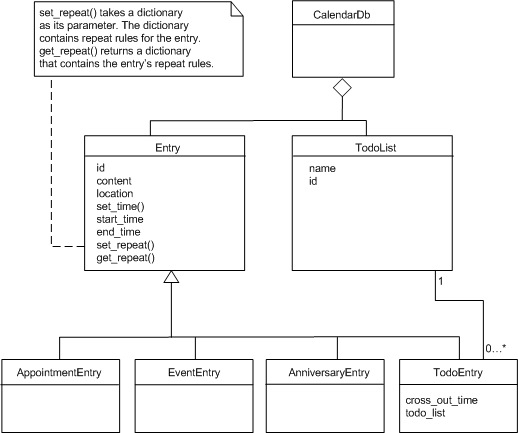
\includegraphics[width=10cm]{libcalendar-1}
\caption{The \module{calendar} module objects}
\label{libcalendar-1}
\end{figure}

Figure \ref{libcalendar-1} demonstrates the relationships of the 
\code{calendar} module objects. 

\subsection{Module Level Functions}
\label{subsec:calendarmodule}
The following free functions - functions that do not belong to any class 
- are defined in the \code{calendar} module:

\begin{funcdesc}{open}{\optional{filename=None, mode=None}}

Opens a calendar database and returns a new \class{CalendarDb} object.

If filename is \code{None}, the default database is opened.

If \var{filename} is given, it should be a full, absolute path name in
Unicode that specifies the calendar database to open. 

\var{mode} can be:

\begin{itemize}
\item \code{None}: Opens an existing calendar database.
\item \code{'c'}: Opens an existing calendar database, or creates it if it doesn't exist.
\item \code{'n'}: Creates a new, empty calendar database. If \var{filename} exists, the previous contents are erased.
\end{itemize}

\end{funcdesc}

\subsection{CalendarDb Objects}
\label{subsec:calendardb}

Calendar entries and todo lists are stored in a calendar database. There is 
one default calendar database but more calendar databases can be created by 
invoking \code{open} with parameters \code{'n' }or \code{'c'}. 

\begin{classdesc*}{CalendarDb}
\class{CalendarDb} objects have the following methods:

\begin{methoddesc}[CalendarDb]{add_appointment}{}

Creates and returns a new appointment entry \class{AppointmentEntry}. The 
entry is not added and saved into the database until \code{Entry.commit} is 
called.

\end{methoddesc}

\begin{methoddesc}[CalendarDb]{add_event}{}

Creates and returns a new event entry \class{EventEntry}. The entry is not added 
and saved into the database until \code{Entry.commit} is called.

\end{methoddesc}

\begin{methoddesc}[CalendarDb]{add_anniversary}{}

Creates and returns a new anniversary entry \class{AnniversaryEntry}. The entry 
is not added and saved into the database until \code{Entry.commit} is called.

\end{methoddesc}

\begin{methoddesc}[CalendarDb]{add_todo}{}

Creates and returns new todo entry \class{TodoEntry}. The entry is not added and 
saved into the database until \code{Entry.commit} is called.

\end{methoddesc}

\begin{methoddesc}[CalendarDb]{find_instances}{start_date, end_date, search_str=u''\optional{ ,appointments=0,events=0,anniversaries=0,todos=0}}

The parameters for this function include the start date, end date, search 
string, and optional parameters. The optional parameters define the entry 
types to be included into the search. By default all entry types are 
included. Returns a list that contains \class{Entry} instances found in the 
search. An instance is a dictionary that contains the entry ID and the 
datetime value. An entry may have several instances if it is repeated, for 
example once every week, etc. However, all the returned instances occur on 
the same day, i.e. on the first day between the start and end datetime 
values that contains instances. To search all instances between the initial 
start and end datetime values, you may have to execute several searches and 
change the start datetime value for each search. A match is detected if the 
search string is a substring of an entry's content. 

\end{methoddesc}

\begin{methoddesc}[CalendarDb]{monthly_instances}{month, appointments=0, events=0, anniversaries=0, todos=0}

The parameters for this function include \var{month} (float) and 
optional parameters. The optional parameters define the entry types to be 
returned. Returns a list that contains entry instances occurring during the 
specified calendar month.

\end{methoddesc}

\begin{methoddesc}[CalendarDb]{daily_instances}{day, appointments=0, events=0, anniversaries=0, todos=0}

The parameters for this function include \var{day} (float) and 
optional parameters. The optional parameters define the entry types to be 
returned. Returns a list that contains entry instances occurring on the 
specified day.

\end{methoddesc}

\begin{methoddesc}[CalendarDb]{add_todo_list}{\optional{name=None}}

Creates a new todo list. \var{name} sets the name of the todo list 
(Unicode). Returns the ID of the created todo list.

\end{methoddesc}

\begin{methoddesc}[CalendarDb]{export_vcalendars}{(int,...)}

Returns a \code{vcalendar} string that contains the specified entries in 
vCalendar format. The parameter for this function is a tuple that contains 
the entry IDs of the exported entries.

\end{methoddesc}

\begin{methoddesc}[CalendarDb]{import_vcalendars}{string}

Imports \code{vcalendar} entries, given in the string parameter, to the 
database. Returns a tuple that contains the unique IDs of the imported 
entries.

\end{methoddesc}

\begin{memberdesc}[CalendarDb]{todo_lists}

Contains a dictionary-like \code{TodoListDict} object for accessing
the todo lists of this database.

\end{memberdesc}

\begin{methoddesc}[CalendarDb]{__delitem__}{id}

Deletes the given calendar \code{Entry} from the database. \code{id} is the 
unique ID of the calendar \code{Entry}.

\end{methoddesc}

\begin{methoddesc}[CalendarDb]{__getitem__}{id}

Returns a calendar \code{Entry} object indicated by the unique ID. The returned 
object can be one of the following: \class{AppointmentEntry}, 
\class{EventEntry}, \class{AnniversaryEntry}, or \class{TodoEntry}. \code{id} is 
the unique ID of the calendar \code{Entry}. 

\end{methoddesc}

\begin{methoddesc}[CalendarDb]{compact}{}

Compacts the database file. The returned value (integer) indicates the 
success of compaction; a value other than zero means that the compaction was 
successful.

\end{methoddesc}

\end{classdesc*}

\subsection{Entry Objects}
\label{subsec:entry}

An \class{Entry} object represents a live view into the state of a single 
entry in the database. You can access the entries with an entry's unique ID. 
If you create a new entry using \code{db.add_appointment} etc., it is 
saved into the database only if you call the entry's \code{commit} method. 
In case an entry is already saved into the database, the autocommit mode is 
on by default and all the changes are automatically saved into the database, 
unless you call the entry's \code{begin} method. If you call the entry's 
\code{begin} method, the changes are not saved into the database until you 
call the entry's \code{commit} method. 

Database entries cannot be locked. In other words, other applications are 
able to make changes to the database entries you are using (not directly to 
the \class{EntryObjects} you are using, but to their representation in the 
database) at the same time you are modifying them, even if you use 
\code{begin} and \code{commit} methods. 

\begin{classdesc*}{Entry}
\class{Entry} objects have the following methods and properties:

\begin{memberdesc}[Entry]{content}

Sets or returns the entry's content text (Unicode).

\end{memberdesc}

\begin{methoddesc}[Entry]{commit}{}

Saves the entry or in case of a new entry adds the entry into the database. 
Note that this can be called only in case of a new entry, created with 
\code{db.add_appointment} etc., or after \code{begin} is called. 

\end{methoddesc}

\begin{methoddesc}[Entry]{rollback}{}

Undoes the changes made after last \code{commit}.

\end{methoddesc}

\begin{methoddesc}[Entry]{set_repeat}{dictionary}

Sets the repeat data of the entry. \var{dictionary} is a repeat data dictionary 
that contains all the repeat rules. For more information on repeat rules, see 
Section \ref{subsec:repeat}, Repeat Rules.

\end{methoddesc}

\begin{methoddesc}[Entry]{get_repeat}{}

Returns the repeat data dictionary of the entry.

\end{methoddesc}

\begin{memberdesc}[Entry]{location}

Sets or returns the entry's location data (Unicode), for example meeting 
room information. 

\end{memberdesc}

\begin{methoddesc}[Entry]{set_time}{start\optional{, end}}

Sets the start and end datetime values of the entry (floats). If only one 
parameter is given, the other will have the same value. 

In case of events, anniversaries, and todo entries the datetime values are 
truncated to corresponding date values.

\class{TodoEntries} can be made undated with 
\code{TodoEntry.set_time(None)}. Making the todo entry undated means 
removing the start and end date and all the repeat rules.

\end{methoddesc}

\begin{memberdesc}[Entry]{start_time}

The start datetime value (float) of the entry or \code{None} if 
the start datetime of the entry is not set.

\end{memberdesc}

\begin{memberdesc}[Entry]{end_time}

The end datetime value (float) of the entry or \code{None} if the 
end datetime of the entry is not set.

\end{memberdesc}

\begin{memberdesc}[Entry]{id}

The unique ID of the entry.

\end{memberdesc}

\begin{memberdesc}[Entry]{last_modified}

The datetime value (float) of the entry's last modification in 
universal time.

\end{memberdesc}

\begin{memberdesc}[Entry]{alarm}

The alarm datetime value (float) for the entry. \code{None} if \code{alarm} is 
not set. Alternatively removes the alarm if the value is set to \code{None}. 

Alarms can be set to all \class{Entry} types. However, only alarms set to 
Appointments and Anniversaries will actually cause an alarm; this is similar 
to the Calendar application in your Nokia device, which allows you to set an 
alarm only for Meetings and Anniversaries. In addition, alarms set to any 
entries residing in a database other than the default database do not cause 
actual alarms either.

\end{memberdesc}

\begin{memberdesc}[Entry]{priority}

The priority of the entry, which can be an integer ranging from 0 to 255. Native 
Phonebook and Calendar applications in Nokia devices use value 1 for high 
priority, 2 for normal priority, and 3 for low priority. 

\end{memberdesc}

\begin{memberdesc}[Entry]{crossed_out}

The crossed out value of an entry. A value that is interpreted as false means 
that the entry is not crossed out, whereas a value that is interpreted as true 
means that the entry is crossed out. Note that \class{TodoEntries} must also 
have a cross-out time while the other entry types cannot have one. If 
\class{TodoEntry} is crossed out using this method, the moment of crossing out 
is set to the cross-out time of the \class{TodoEntry}. See also Section 
\ref{subsubsec:todoentry}, TodoEntry, \code{cross_out_time}.

\end{memberdesc}

\begin{memberdesc}[Entry]{replication}

Sets or returns the entry's replication status, which can be one of the 
following: \code{'open'}, \code{'private',} or \code{'restricted'}.

\end{memberdesc}

\begin{methoddesc}[Entry]{as_vcalendar}{}

Returns this entry as a vCalendar string.

\end{methoddesc}

\end{classdesc*}

\subsubsection{AppointmentEntry Objects}
\label{subsubsec:appointmententry}

\begin{classdesc*}{AppointmentEntry}
\end{classdesc*}

\class{AppointmentEntry} class contains no additional methods compared to 
the \class{Entry} class from which it is derived.

\subsubsection{EventEntry}
\label{subsubsec:evententry}

\begin{classdesc*}{EventEntry}
\end{classdesc*}

\class{EventEntry} class contains no additional methods compared to the 
\class{Entry} class from which it is derived.

\subsubsection{AnniversaryEntry}
\label{subsubsec:anniversaryentry}

\begin{classdesc*}{AnniversaryEntry}
\end{classdesc*}

\class{AnniversaryEntry} class contains no additional methods compared to 
the \class{Entry} class from which it is derived.

\subsubsection{TodoEntry}
\label{subsubsec:todoentry}

\class{TodoEntry}objects represent todo entry types. They have additional 
properties compared to the \class{Entry} class from which they are derived.

\begin{classdesc*}{TodoEntry}
\class{TodoEntry}objects have the following additional properties:

\begin{memberdesc}[TodoEntry]{cross_out_time}

The cross-out date value of the entry. The value can be \code{None} meaning that 
the entry is not crossed out, or the cross-out date (float). The set value must 
be date (float). Setting a cross-out time also crosses out the entry. See also 
Section \ref{subsec:entry}, Entry Object, \code{crossed_out}.

\end{memberdesc}

\begin{memberdesc}[TodoEntry]{todo_list}

The ID of the todo list to which this entry belongs.

\end{memberdesc}

\end{classdesc*}

\subsubsection{TodoListDict}
\label{subsubsec:todolistdict}

\class{TodoListDict} objects are dictionary-like objects that enable 
accessing todo lists. 

\begin{classdesc*}{TodoListDict}
\class{TodoListDict} objects have the following property:

\begin{memberdesc}[TodoListDict]{default_list}

The ID of the default todo list.

\end{memberdesc}

\end{classdesc*}

\subsubsection{TodoList}
\label{subsubsec:todolist}

\class{TodoList} objects are dictionary-like objects that enable 
accessesing todo lists. 

\begin{classdesc*}{TodoList}
\code{TodoList} objects have the following properties:

\begin{memberdesc}[TodoList]{name}

The name of the todo list as a Unicode string.

\end{memberdesc}

\begin{memberdesc}[TodoList]{id}

Returns the ID of the todo list as an integer.

\end{memberdesc}

\end{classdesc*}

\subsection{Repeat Rules}
\label{subsec:repeat}

Repeat rules specify an entry's repeat status, that is, the recurrence of 
the entry. There are six repeat types: 

\begin{itemize}
\item \code{daily}: repeated daily
\item \code{weekly}: repeat on the specified days of the week, such as Monday and Wednesday, etc.
\item \code{monthly_by_dates}: repeat monthly on the specified dates, such as the 15th and 17th day of the month
\item \code{monthly_by_days}: repeat monthly on the specified days, such as the fourth Wednesday of the month, or the last Monday of the month
\item \code{yearly_by_date}: repeat yearly on the specified date, such as December 24
\item \code{yearly_by_day}: repeat yearly on the specified day, such as every third Tuesday of May
\end{itemize}

There are exceptions to repeat rules. For example, you can specify the 
datetime value (float) in such a way that the entry is not repeated on a 
specific day even if the repeat rule would specify otherwise.

You must set the start and end dates (floats) of the repeat. The end date 
can also be set to \code{None} to indicate that the repeating continues 
forever. You can set \code{interval} defining how often the repeat occurs, 
for example in a daily repeat: \code{1} means every day, \code{2} means 
every second day, etc. You can also set the \code{days} specifier which 
lets you explicitly specify the repeat days; for example in a weekly repeat 
you can set \code{"days":[0,2]} which sets the repeat to occur on Mondays 
and Wednesdays. If you do not set the \code{days} specifier, the repeat 
days are calculated automatically based on the start date.

You can modify repeat data by calling \code{rep_data = 
entry.get_repeat()}, then making changes to \code{rep_data} 
dictionary, and then calling \code{entry.set_repeat(rep_data)}.

Repeating can be cancelled by calling \code{entry.set_repeat} with a 
parameter that is interpreted to be false, such as 
\code{entry.set_repeat(None)}.

Repeat definition examples:

\begin{verbatim}

repeat = {"type":"daily", #repeat type
          "exceptions":[exception_day, exception_day+2*24*60*60],  
          #no appointment on those days
          "start":appt_start_date, #start of the repeat
          "end":appt_start_date+30*24*60*60, #end of the repeat
          "interval":1} #interval (1=every day, 2=every second day etc.)

repeat = {"type":"weekly", #repeat type
          "days":[0,1], #which days in a week (Monday, Tuesday)
          "exceptions":[exception_day], #no appointment on that day
          "start":appt_start_date, #start of the repeat
          "end":appt_start_date+30*24*60*60, #end of the repeat
          "interval":1}  
          #interval (1=every week, 2=every second week etc.) 

repeat = {"type":"monthly_by_days", #repeat type
          # appointments on second Tuesday and last Monday of the month
          "days":[{"week":1, "day":1},{"week":4, "day":0}],
          "exceptions":[exception_day], #no appointment on that day 
          "start":appt_start_date, #start of the repeat
          "end":appt_start_date+30*24*60*60, #end of the repeat
          "interval":1}  
          #interval (1=every month, 2=every second month etc.)

repeat = {"type":"monthly_by_dates", #repeat type
          "days":[0,15],  
          # appointments on the 1st and 16th day of the month.
          "exceptions":[exception_day], #no appointment on that day
          "start":appt_start_date, #start of the repeat
          "end":appt_start_date+30*24*60*60, #end of the repeat
          "interval":1}  
          #interval (1=every month, 2=every second month etc.)

repeat = {"type":"yearly_by_date", #repeat type
          "exceptions":[exception_day], #no appointment on that day 
          "start":appt_start_date, #start of the repeat
          "end":appt_start_date+3*365*24*60*60, #end of the repeat
          "interval":1}  
          #interval (1=every year, 2=every second year etc.)

repeat = {"type":"yearly_by_day", #repeat type
          # appointments on the second Tuesday of February
          "days":{"day":1, "week":1, "month":1},
          "exceptions":[exception_day], #no appointment on that day 
          "start":appt_start_date, #start of the repeat
          "end":appt_start_date+3*365*24*60*60, #end of the repeat
          "interval":1}  
          #interval (1=every year, 2=every second year etc.)

\end{verbatim}

% Copyright (c) 2006 Nokia Corporation
%
% Licensed under the Apache License, Version 2.0 (the "License");
% you may not use this file except in compliance with the License.
% You may obtain a copy of the License at
%
%     http://www.apache.org/licenses/LICENSE-2.0
%
% Unless required by applicable law or agreed to in writing, software
% distributed under the License is distributed on an "AS IS" BASIS,
% WITHOUT WARRANTIES OR CONDITIONS OF ANY KIND, either express or implied.
% See the License for the specific language governing permissions and
% limitations under the License.

\section{\module{calendar for EKA2} ---
  Access to calendar related services}
\label{sec:calendareka2}

\declaremodule{extension}{calendar}
\platform{S60}
\modulesynopsis{A calendar related services package.}

The \module{calendar} module offers an API to calendar services. The 
\module{calendar} module represents a Symbian agenda database as a 
dictionary-like \class{CalendarDb} object, which contains \class{Entry}
objects and which is indexed using the unique IDs of those objects. There 
are five types of entry objects: \class{AppointmentEntry}, 
\class{EventEntry}, \class{AnniversaryEntry}, \class{ReminderEntry},
 and \class{TodoEntry}. 

\class{CalendarDb} objects represent a live view into the database. If an 
entry is changed outside your Python application, the changes are visible 
immediately, and conversely any changes you commit into the database are 
visible immediately to other applications. 

All time parameters use Unix time unless stated otherwise. For more 
information on Unix time, see Section \ref{subsec:datetime}, 
Date and Time.

\subsection{Module Level Functions}
\label{subsec:calendarmodule}
The following free functions - functions that do not belong to any class 
- are defined in the \code{calendar} module:

\begin{funcdesc}{open}{\optional{filename=None, mode=None}}

Opens a calendar database and returns a new \class{CalendarDb} object.

If filename is \code{None}, the default database is opened.

If \var{filename} is given, it should contain drive letter, colon and file's name, 
but no absolute path.

\var{mode} can be:

\begin{itemize}
\item \code{None}: Opens an existing calendar database.
\item \code{'c'}: Opens an existing calendar database, or creates it if it doesn't exist.
\item \code{'n'}: Creates a new, empty calendar database. If \var{filename} exists, the previous contents are erased.
\end{itemize}

\end{funcdesc}

\subsection{CalendarDb Objects}
\label{subsec:calendardb}

Calendar entries are stored in a calendar database. There is 
one default calendar database but more calendar databases can be created by 
invoking \code{open} with parameters \code{'n' }or \code{'c'}. 

\begin{classdesc*}{CalendarDb}
\class{CalendarDb} objects have the following methods:

\begin{methoddesc}[CalendarDb]{add_appointment}{}

Creates and returns a new appointment entry \class{AppointmentEntry}. The 
entry is not added and saved into the database until \code{Entry.commit} is 
called.

\end{methoddesc}

\begin{methoddesc}[CalendarDb]{add_event}{}

Creates and returns a new event entry \class{EventEntry}. The entry is not added 
and saved into the database until \code{Entry.commit} is called.

\end{methoddesc}

\begin{methoddesc}[CalendarDb]{add_anniversary}{}

Creates and returns a new anniversary entry \class{AnniversaryEntry}. The entry 
is not added and saved into the database until \code{Entry.commit} is called.

\end{methoddesc}

\begin{methoddesc}[CalendarDb]{add_todo}{}

Creates and returns new todo entry \class{TodoEntry}. The entry is not added and 
saved into the database until \code{Entry.commit} is called.

\end{methoddesc}

\begin{methoddesc}[CalendarDb]{add_reminder}{}

Creates and returns new reminder entry \class{ReminderEntry}. The entry is not added and 
saved into the database until \code{Entry.commit} is called.

\end{methoddesc}

\begin{methoddesc}[CalendarDb]{find_instances}{start_date, end_date, search_str=u''\optional{ ,appointments=0,events=0,anniversaries=0,todos=0,reminders=0}}

The parameters for this function include the start date, end date, search 
string, and optional parameters. The optional parameters define the entry 
types to be included into the search. By default all entry types are 
included. Returns a list that contains \class{Entry} instances found in the 
search. An instance is a dictionary that contains the entry ID and the 
datetime value. An entry may have several instances if it is repeated, for 
example once every week, etc. 

\end{methoddesc}

\begin{methoddesc}[CalendarDb]{monthly_instances}{month, appointments=0, events=0, anniversaries=0, todos=0, reminders=0}

The parameters for this function include \var{month} (float) and 
optional parameters. The optional parameters define the entry types to be 
returned. Returns a list that contains entry instances occurring during the 
specified calendar month.

\end{methoddesc}

\begin{methoddesc}[CalendarDb]{daily_instances}{day, appointments=0, events=0, anniversaries=0, todos=0}

The parameters for this function include \var{day} (float) and 
optional parameters. The optional parameters define the entry types to be 
returned. Returns a list that contains entry instances occurring on the 
specified day.

\end{methoddesc}

\begin{methoddesc}[CalendarDb]{export_vcalendars}{(int,...)}

Returns a \code{vcalendar} string that contains the specified entries in 
vCalendar format. The parameter for this function is a tuple that contains 
the entry IDs of the exported entries.

\end{methoddesc}

\begin{methoddesc}[CalendarDb]{import_vcalendars}{string}

Imports \code{vcalendar} entries, given in the string parameter, to the 
database. Returns a list that contains the unique IDs of the imported 
entries.

\end{methoddesc}

\begin{methoddesc}[CalendarDb]{__delitem__}{id}

Deletes the given calendar \code{Entry} from the database. \code{id} is the 
unique ID of the calendar \code{Entry}.

\end{methoddesc}

\begin{methoddesc}[CalendarDb]{__getitem__}{id}

Returns a calendar \code{Entry} object indicated by the unique ID. The returned 
object can be one of the following: \class{AppointmentEntry}, 
\class{EventEntry}, \class{AnniversaryEntry}, \class{ReminderEntry}, 
or \class{TodoEntry}. \code{id} is the unique ID of the calendar \code{Entry}. 

\end{methoddesc}

\end{classdesc*}

\subsection{Entry Objects}
\label{subsec:entry}

An \class{Entry} object represents a live view into the state of a single 
entry in the database. You can access the entries with an entry's unique ID. 
If you create a new entry using \code{db.add_appointment} etc., it is 
saved into the database only if you call the entry's \code{commit} method. 
In case an entry is already saved into the database, the autocommit mode is 
on by default and all the changes are automatically saved into the database, 
unless you call the entry's \code{begin} method. If you call the entry's 
\code{begin} method, the changes are not saved into the database until you 
call the entry's \code{commit} method. 

Database entries cannot be locked. In other words, other applications are 
able to make changes to the database entries you are using (not directly to 
the \class{EntryObjects} you are using, but to their representation in the 
database) at the same time you are modifying them, even if you use 
\code{begin} and \code{commit} methods. 

\begin{classdesc*}{Entry}
\class{Entry} objects have the following methods and properties:

\begin{memberdesc}[Entry]{content}

Sets or returns the entry's content text (Unicode).

\end{memberdesc}

\begin{methoddesc}[Entry]{commit}{}

Saves the entry or in case of a new entry adds the entry into the database. 
Note that this can be called only in case of a new entry, created with 
\code{db.add_appointment} etc., or after \code{begin} is called. 

\end{methoddesc}

\begin{methoddesc}[Entry]{rollback}{}

Undoes the changes made after last \code{commit}.

\end{methoddesc}

\begin{methoddesc}[Entry]{set_repeat}{dictionary}

Sets the repeat data of the entry. \var{dictionary} is a repeat data dictionary 
that contains all the repeat rules. For more information on repeat rules, see 
Section \ref{subsec:repeat}, Repeat Rules.

\end{methoddesc}

\begin{methoddesc}[Entry]{get_repeat}{}

Returns the repeat data dictionary of the entry.

\end{methoddesc}

\begin{memberdesc}[Entry]{location}

Sets or returns the entry's location data (Unicode), for example meeting 
room information. 

\end{memberdesc}

\begin{methoddesc}[Entry]{set_time}{start\optional{, end}}

Sets the start and end datetime values of the entry (floats). If only one 
parameter is given, the other will have the same value. 

In case of events, anniversaries, and todo entries the datetime values are 
truncated to corresponding date values.

\class{TodoEntries} can be made undated with 
\code{TodoEntry.set_time(None)}. Making the todo entry undated means 
removing the start and end date and all the repeat rules.

\end{methoddesc}

\begin{memberdesc}[Entry]{start_time}

The start datetime value (float) of the entry or \code{None} if 
the start datetime of the entry is not set.

\end{memberdesc}

\begin{memberdesc}[Entry]{end_time}

The end datetime value (float) of the entry or \code{None} if the 
end datetime of the entry is not set.

\end{memberdesc}

\begin{memberdesc}[Entry]{id}

The unique ID of the entry.

\end{memberdesc}

\begin{memberdesc}[Entry]{last_modified}

The datetime value (float) of the entry's last modification in 
universal time.

\end{memberdesc}

\begin{memberdesc}[Entry]{originating}

An integer value indicating if the entry is an originating entry
or a modifying entry.

\end{memberdesc}

\begin{memberdesc}[Entry]{alarm}

The alarm datetime value (float) for the entry. \code{None} if \code{alarm} is 
not set. Alternatively removes the alarm if the value is set to \code{None}. 

Alarms can be set to all \class{Entry} types. However, only alarms set to 
Appointments and Anniversaries will actually cause an alarm; this is similar 
to the Calendar application in your Nokia device, which allows you to set an 
alarm only for Meetings and Anniversaries. In addition, alarms set to any 
entries residing in a database other than the default database do not cause 
actual alarms either.

\end{memberdesc}

\begin{memberdesc}[Entry]{priority}

The priority of the entry, which can be an integer ranging from 0 to 255. Native 
Phonebook and Calendar applications in Nokia devices use value 1 for high 
priority, 2 for normal priority, and 3 for low priority. 

\end{memberdesc}

\begin{memberdesc}[Entry]{crossed_out}

The crossed out value of an entry. Only valid for todo entries.
A value that is interpreted as false means 
that the entry is not crossed out, whereas a value that is interpreted as true 
means that the entry is crossed out. Note that \class{TodoEntries} must also 
have a cross-out time. If \class{TodoEntry} is crossed out using this method, 
the moment of crossing out is set to the cross-out time of the \class{TodoEntry}. 
See also Section \ref{subsubsec:todoentry}, TodoEntry, \code{cross_out_time}.

\end{memberdesc}

\begin{memberdesc}[Entry]{replication}

Sets or returns the entry's replication status, which can be one of the 
following: \code{'open'}, \code{'private',} or \code{'restricted'}.

\end{memberdesc}

\begin{methoddesc}[Entry]{as_vcalendar}{}

Returns this entry as a vCalendar string.

\end{methoddesc}

\end{classdesc*}

\subsubsection{AppointmentEntry Objects}
\label{subsubsec:appointmententry}

\begin{classdesc*}{AppointmentEntry}
\end{classdesc*}

\class{AppointmentEntry} class contains no additional methods compared to 
the \class{Entry} class from which it is derived.

\subsubsection{EventEntry}
\label{subsubsec:evententry}

\begin{classdesc*}{EventEntry}
\end{classdesc*}

\class{EventEntry} class contains no additional methods compared to the 
\class{Entry} class from which it is derived.

\subsubsection{AnniversaryEntry}
\label{subsubsec:anniversaryentry}

\begin{classdesc*}{AnniversaryEntry}
\end{classdesc*}

\class{AnniversaryEntry} class contains no additional methods compared to 
the \class{Entry} class from which it is derived.

\subsubsection{ReminderEntry}
\label{subsubsec:reminderentry}

\begin{classdesc*}{ReminderEntry}
\end{classdesc*}

\class{ReminderEntry} class contains no additional methods compared to 
the \class{Entry} class from which it is derived.

\subsubsection{TodoEntry}
\label{subsubsec:todoentry}

\class{TodoEntry}objects represent todo entry types. They have additional 
properties compared to the \class{Entry} class from which they are derived.

\begin{classdesc*}{TodoEntry}
\class{TodoEntry}objects have the following additional properties:

\begin{memberdesc}[TodoEntry]{cross_out_time}

The cross-out date value of the entry. The value can be \code{None} meaning that 
the entry is not crossed out, or the cross-out date (float). The set value must 
be date (float). Setting a cross-out time also crosses out the entry. See also 
Section \ref{subsec:entry}, Entry Object, \code{crossed_out}.

\end{memberdesc}

\end{classdesc*}


\subsection{Repeat Rules}
\label{subsec:repeat}

Repeat rules specify an entry's repeat status, that is, the recurrence of 
the entry. There are six repeat types: 

\begin{itemize}
\item \code{daily}: repeated daily
\item \code{weekly}: repeat on the specified days of the week, such as Monday and Wednesday, etc.
\item \code{monthly_by_dates}: repeat monthly on the specified dates, such as the 15th and 17th day of the month
\item \code{monthly_by_days}: repeat monthly on the specified days, such as the fourth Wednesday of the month, or the last Monday of the month
\item \code{yearly_by_date}: repeat yearly on the specified date, such as December 24
\item \code{yearly_by_day}: repeat yearly on the specified day, such as every third Tuesday of May
\end{itemize}

There are exceptions to repeat rules. For example, you can specify the 
datetime value (float) in such a way that the entry is not repeated on a 
specific day even if the repeat rule would specify otherwise.

You must set the start and end dates (floats) of the repeat. The end date 
can also be set to \code{None} to indicate that the repeating continues 
forever. You can set \code{interval} defining how often the repeat occurs, 
for example in a daily repeat: \code{1} means every day, \code{2} means 
every second day, etc. You can also set the \code{days} specifier which 
lets you explicitly specify the repeat days; for example in a weekly repeat 
you can set \code{"days":[0,2]} which sets the repeat to occur on Mondays 
and Wednesdays. If you do not set the \code{days} specifier, the repeat 
days are calculated automatically based on the start date.

You can modify repeat data by calling \code{rep_data = 
entry.get_repeat()}, then making changes to \code{rep_data} 
dictionary, and then calling \code{entry.set_repeat(rep_data)}.

Repeating can be cancelled by calling \code{entry.set_repeat} with a 
parameter that is interpreted to be false, such as 
\code{entry.set_repeat(None)}.

Repeat definition examples:

\begin{verbatim}

repeat = {"type":"daily", #repeat type
          "exceptions":[exception_day, exception_day+2*24*60*60],  
          #no appointment on those days
          "start":appt_start_date, #start of the repeat
          "end":appt_start_date+30*24*60*60, #end of the repeat
          "interval":1} #interval (1=every day, 2=every second day etc.)

repeat = {"type":"weekly", #repeat type
          "days":[0,1], #which days in a week (Monday, Tuesday)
          "exceptions":[exception_day], #no appointment on that day
          "start":appt_start_date, #start of the repeat
          "end":appt_start_date+30*24*60*60, #end of the repeat
          "interval":1}  
          #interval (1=every week, 2=every second week etc.) 

repeat = {"type":"monthly_by_days", #repeat type
          # appointments on second Tuesday and last Monday of the month
          "days":[{"week":1, "day":1},{"week":4, "day":0}],
          "exceptions":[exception_day], #no appointment on that day 
          "start":appt_start_date, #start of the repeat
          "end":appt_start_date+30*24*60*60, #end of the repeat
          "interval":1}  
          #interval (1=every month, 2=every second month etc.)

repeat = {"type":"monthly_by_dates", #repeat type
          "days":[0,15],  
          # appointments on the 1st and 16th day of the month.
          "exceptions":[exception_day], #no appointment on that day
          "start":appt_start_date, #start of the repeat
          "end":appt_start_date+30*24*60*60, #end of the repeat
          "interval":1}  
          #interval (1=every month, 2=every second month etc.)

repeat = {"type":"yearly_by_date", #repeat type
          "exceptions":[exception_day], #no appointment on that day 
          "start":appt_start_date, #start of the repeat
          "end":appt_start_date+3*365*24*60*60, #end of the repeat
          "interval":1}  
          #interval (1=every year, 2=every second year etc.)

repeat = {"type":"yearly_by_day", #repeat type
          # appointments on the second Tuesday of February
          "days":{"day":1, "week":1, "month":1},
          "exceptions":[exception_day], #no appointment on that day 
          "start":appt_start_date, #start of the repeat
          "end":appt_start_date+3*365*24*60*60, #end of the repeat
          "interval":1}  
          #interval (1=every year, 2=every second year etc.)

\end{verbatim}

% Copyright (c) 2005 Nokia Corporation
%
% Licensed under the Apache License, Version 2.0 (the "License");
% you may not use this file except in compliance with the License.
% You may obtain a copy of the License at
%
%     http://www.apache.org/licenses/LICENSE-2.0
%
% Unless required by applicable law or agreed to in writing, software
% distributed under the License is distributed on an "AS IS" BASIS,
% WITHOUT WARRANTIES OR CONDITIONS OF ANY KIND, either express or implied.
% See the License for the specific language governing permissions and
% limitations under the License.

\section{\module{e32db} ---
  Interface to the Symbian native DB}
\label{sec:e32db}

\declaremodule{extension}{e32db}
\platform{S60}
\modulesynopsis{Interface to the Symbian native DB}

\label{sec:mylabel3}
The \module{e32db} module provides an API for relational database 
manipulation with a restricted SQL syntax. For details of DBMS support, see 
the S60 SDK documentation. For examples on using this module, see \cite{PyS60Prog}.

The \module{e32db} module defines the following functions:

\begin{funcdesc}{format_rawtime}{timevalue}
Formats \var{timevalue} (Symbian time) according to the current 
system's date/time formatting rules and returns it as a Unicode string.
\end{funcdesc}

\begin{funcdesc}{format_time}{timevalue}
Formats \var{timevalue} according to the current system's date/time 
formatting rules and returns it as a Unicode string.
\end{funcdesc}

\subsection{Dbms Objects}
\label{subsec:mylabel13}

\begin{classdesc}{Dbms}{}
Creates a Dbms object. Dbms objects support basic 
operations on a database. 
\end{classdesc}

Dbms objects have the following methods:

\begin{methoddesc}[Dbms]{begin}{}
Begins a transaction on the database.
\end{methoddesc}

\begin{methoddesc}[Dbms]{close}{}
Closes the database object. It is safe to try to close a database object 
even if it is not open.
\end{methoddesc}

\begin{methoddesc}[Dbms]{commit}{}
Commits the current transaction.
\end{methoddesc}

\begin{methoddesc}[Dbms]{compact}{}
Compacts the database, reclaiming unused space in the database file. 
\end{methoddesc}

\begin{methoddesc}[Dbms]{create}{dbname}
Creates a database with path \var{dbname}.
\end{methoddesc}

\begin{methoddesc}[Dbms]{execute}{query}
Executes an SQL \var{query}. On success, returns \code{0} if a DDL
(SQL schema update) statement was executed. Returns the number of rows
inserted, updated, or deleted, if a DML (SQL data update) statement
was executed.
\end{methoddesc}

\begin{methoddesc}[Dbms]{open}{dbname}
Opens the database in file \var{dbname}. This should be a full 
Unicode path name, for example, \code{u'c:\e\e foo.db'}.
\end{methoddesc}

\begin{methoddesc}[Dbms]{rollback}{}
Rolls back the current transaction.
\end{methoddesc}

\subsection{DB_view Objects}
\label{subsec:mylabel14}

\begin{classdesc}{Db_view}{}
Creates a \class{Db_view} object. \class{DB_view} objects generate 
rowsets from a SQL query. They provide functions to parse and evaluate the 
rowsets.
\end{classdesc}

Db_view objects have the following methods:

\begin{methoddesc}[Db_view]{col}{column}
Returns the value in \var{column}. The first column of the rowset has the index 
\code{1}. If the type of the column is not supported, a \exception{TypeError} is 
raised. See Table \ref{tab:sqltypes} for a list of supported data types.
\end{methoddesc}

\begin{methoddesc}[Db_view]{col_count}{}
Returns the number of columns defined in the rowset.
\end{methoddesc}

\begin{methoddesc}[Db_view]{col_length}{column}
Gets the length of the value in \var{column}. Empty columns have 
a length of zero; non-empty numerical and date/time columns have a length of 
1. For text columns, the length is the character count, and for binary 
columns, the length is the byte count.
\end{methoddesc}

\begin{methoddesc}[Db_view]{col_raw}{column}
Extracts the value of \var{column} as raw binary data, and 
returns it as a Python string. The first column of the rowset has the index 
1. See Table \ref{tab:sqltypes} for a list of supported data types.
\end{methoddesc}

\begin{methoddesc}[Db_view]{col_rawtime}{column}
Extracts the value of a date/time column at index \var{column} as a
long integer, which represents the raw Symbian time value. The first
column of the rowset has the index 1.  See Table \ref{tab:sqltypes} for a list of the
supported data types.
\end{methoddesc}

\begin{methoddesc}[Db_view]{col_type}{column}
Returns the numeric type of the given column as an integer from a 
Symbian-specific list of types. This function is used in the implementation 
of method \method{col}.
\end{methoddesc}

\begin{methoddesc}[Db_view]{count_line}{}
Returns the number of rows available in the rowset.
\end{methoddesc}

\begin{methoddesc}[Db_view]{first_line}{}
Positions the cursor on the first row in the rowset.
\end{methoddesc}

\begin{methoddesc}[Db_view]{get_line}{}
Gets the current row data for access.
\end{methoddesc}

\begin{methoddesc}[Db_view]{is_col_null}{column}
Tests whether \var{column} is empty. Empty columns can be 
accessed like normal columns. Empty numerical columns return a \code{0} or 
an equivalent value, and text and binary columns have a zero length.
\end{methoddesc}

\begin{methoddesc}[Db_view]{next_line}{}
Moves the cursor to the next row in the rowset.
\end{methoddesc}

\begin{methoddesc}[Db_view]{prepare}{db, query}
Prepares the view object for evaluating an SQL select statement. 
\var{db} is a \class{Dbms} object and \var{query}
the SQL query to be executed.
\end{methoddesc}

\subsection{Mapping Between SQL and Python Data Types }
\label{subsec:mapping}
See Table \ref{tab:sqltypes} for a summary of mapping between SQL and 
Python data types. The \method{col} function can extract any value except 
\code{LONG VARBINARY} and return it as the proper Python value. In 
addition, the \method{col_raw} function can extract any column type 
except \code{LONG VARCHAR} and \code{LONG VARBINARY} as raw binary data 
and return it as a Python string.

Inserting, updating, or searching for \code{BINARY}, \code{VARBINARY}, 
or \code{LONG VARBINARY} values is not supported. \code{BINARY} and 
\code{VARBINARY} values can be read with \method{col} or 
\method{col_raw}.

\begin{table}[htbp]
\begin{center}
\begin{tabular}{|p{117pt}|p{144pt}|p{99pt}|p{63pt}|}
\hline
SQL type& 
Symbian column type (in the DBMS C++ API)& 
Python type& 
Supported \\
\hline
\textsf{BIT}& 
\textsf{EDbColBit}& 
\raisebox{-10.50ex}[0cm][0cm]{int}& 
\raisebox{-27.00ex}[0cm][0cm]{yes} \\
\cline{1-2} 
\textsf{TINYINT}& 
\textsf{EDbColInt8}& 
 & 
  \\
\cline{1-2} 
\textsf{UNSIGNED TINYINT}& 
\textsf{EDbColUint8}& 
 & 
  \\
\cline{1-2} 
\textsf{SMALLINT}& 
\textsf{EDbColInt16}& 
 & 
  \\
\cline{1-2} 
\textsf{UNSIGNED SMALLINT}& 
\textsf{EDbColUint16}& 
 & 
  \\
\cline{1-2} 
\textsf{INTEGER}& 
\textsf{EDbColInt32}& 
 & 
  \\
\cline{1-2} 
\textsf{UNSIGNED INTEGER}& 
\textsf{EDbColUint32}& 
 & 
  \\
\cline{1-2} 
\textsf{COUNTER}& 
\textsf{EDbColUint32 (}with the\textsf{ TDbCol::EAutoIncrement }attribute\textsf{)}& 
 & 
  \\
\cline{1-3} 
\textsf{BIGINT}& 
\textsf{EDbColInt64}& 
long& 
  \\
\cline{1-3} 
\textsf{REAL}& 
\textsf{EDbColReal32}& 
\raisebox{-4.50ex}[0cm][0cm]{float  \par }& 
  \\
\cline{1-2} 
\textsf{FLOAT}& 
\raisebox{-3.00ex}[0cm][0cm]{\textsf{EDbColReal64} \par \textsf{}}& 
 & 
  \\
\cline{1-1} 
\textsf{DOUBLE}& 
 & 
 & 
  \\
\cline{1-1} 
\textsf{DOUBLE PRECISION}& 
 & 
 & 
  \\
\cline{1-3} 
\textsf{DATE}& 
\raisebox{-3.00ex}[0cm][0cm]{\textsf{EDbColDateTime} \par \textsf{}}& 
\raisebox{-3.00ex}[0cm][0cm]{float \par (or long, with \textsf{col_rawtime()})}& 
  \\
\cline{1-1} 
\textsf{TIME}& 
 & 
 & 
  \\
\cline{1-1} 
\textsf{TIMESTAMP}& 
 & 
 & 
  \\
\cline{1-3} 
\textsf{CHAR(n)}& 
\raisebox{-1.50ex}[0cm][0cm]{\textsf{EDbColText}}& 
\raisebox{-3.00ex}[0cm][0cm]{Unicode}& 
  \\
\cline{1-1} 
\textsf{VARCHAR(n)}& 
 & 
 & 
  \\
\cline{1-2} 
\textsf{LONG VARCHAR}& 
\textsf{EDbColLongText}& 
 & 
  \\
\hline
\textsf{BINARY(n)}& 
\raisebox{-1.50ex}[0cm][0cm]{\textsf{EDbColBinary} \par \textsf{}}& 
\raisebox{-1.50ex}[0cm][0cm]{str}& 
\raisebox{-1.50ex}[0cm][0cm]{read only} \\
\cline{1-1} 
\textsf{VARBINARY(n)}& 
 & 
 & 
  \\
\hline
\textsf{LONG VARBINARY}& 
\textsf{EDbColLongBinary}& 
n/a& 
no \\
\hline
\end{tabular}
\caption{Mapping between SQL and Python types}
\label{tab:sqltypes}
\end{center}
\end{table}


\subsection{Date and Time Handling}
\label{subsec:mylabel15}
The functions \method{col} and \textsf{format_time} use Unix time, 
seconds since January 1, 1970, 00:00:00 UTC, as the time format. Internally 
the database uses the native Symbian time representation that provides 
greater precision and range than the Unix time. The native Symbian time 
format is a 64-bit value that represents microseconds since January 1st 0 AD 
00:00:00 local time, nominal Gregorian. BC dates are represented by negative 
values. Since converting this format to Unix time and back may cause slight 
round-off errors, you have to use the functions \function{col_rawtime} and 
\function{format_rawtime} if you need to be able to handle these values 
with full precision.

The representation of date and time literals in SQL statements depends on 
the current system date and time format. Note that the only accepted 
ordering of day, month, and year is the one that the system is currently 
configured to use. Dates in other order are rejected. The recommended way to 
form date/time literals for SQL statements is to use the functions 
\function{format_time} or \function{format_rawtime} that format the given 
date/time values properly according to the current system's date/time format 
settings.

% Copyright (c) 2005 Nokia Corporation
%
% Licensed under the Apache License, Version 2.0 (the "License");
% you may not use this file except in compliance with the License.
% You may obtain a copy of the License at
%
%     http://www.apache.org/licenses/LICENSE-2.0
%
% Unless required by applicable law or agreed to in writing, software
% distributed under the License is distributed on an "AS IS" BASIS,
% WITHOUT WARRANTIES OR CONDITIONS OF ANY KIND, either express or implied.
% See the License for the specific language governing permissions and
% limitations under the License.

\section{\module{e32dbm} ---
  DBM implemented using the Symbian native DBMS}
\label{sec:e32dbm}

\declaremodule{}{e32dbm}
\platform{S60}
\modulesynopsis{DBM implemented using the Symbian native DBMS}

The \module{e32dbm} module provides a DBM API that uses the native
Symbian RDBMS as its storage back-end. The module API resembles that
of the \refmodule{gdbm} module. The main differences are:

\begin{itemize}
\item The \method{firstkey()} - \method{nextkey()} interface for iterating through keys is not supported. Use the \code{"for key in db"} idiom or the \method{keys} or \method{keysiter} methods instead.
\item This module supports a more complete set of dictionary features than \refmodule{gdbm}
\item The values are always stored as Unicode, and thus the values returned are Unicode strings even if they were given to the DBM as normal strings.
\end{itemize}
\subsection{Module Level Functions}
\label{subsec:mylabel16}

The \module{e32dbm} defines the following functions:

\begin{funcdesc}{open}{dbname\optional{,flags, mode}}
Opens or creates the given database file and returns an \class{e32dbm}
object.  Note that \var{dbname} should be a full path name, for
example, \textsf{u'c:$\backslash
\backslash $foo.db'}. Flags can be:

\begin{itemize}
\item \code{'r'}: opens an existing database in read-only mode. This is the default value.
\item \code{'w'}: opens an existing database in read-write mode.
\item \code{'c'}: opens a database in read-write mode. Creates a new database if the database does not exist.
\item \code{'n'}: creates a new empty database and opens it in read-write mode.
\end{itemize}

If the character \code{'f'} is appended to flags, the database is opened in \textit{fast mode}. In 
fast mode, updates are written to the database only when one of these 
methods is called: \method{sync}, \method{close}, \method{reorganize}, or 
\method{clear}.
\end{funcdesc}

Since the connection object destructor calls \method{close}, it is not 
strictly necessary to close the database before exiting to ensure that data 
is saved, but it is still good practice to call the \method{close} method 
when you are done with using the database. Closing the database releases the 
lock on the file and allows the file to be reopened or deleted without 
exiting the interpreter.

If you plan to do several updates, it is highly recommended that you open 
the database in fast mode, since inserts and updates are more efficient when 
they are bundled together in a larger transaction. This is especially 
important when you plan to insert large amounts of data, since inserting 
records to \refmodule{e32db} is very slow if done one record at a time.

\subsection{e32dbm Objects}
The \module{e32dbm} objects returned by the \method{open} function support 
most of the standard dictionary methods. The supported dictionary methods 
are:

\begin{itemize}
\item \code{__getitem__}
\item \code{__setitem__}
\item \code{__delitem__}
\item \code{has_key}
\item \code{update}
\item \code{__len__}
\item \code{__iter__}
\item \code{iterkeys}
\item \code{iteritems}
\item \code{itervalues}
\item \code{get}
\item \code{setdefault}
\item \code{pop}
\item \code{popitem}
\item \code{clear}
\end{itemize}

These work the same way as the corresponding methods in a normal dictionary.

In addition, \class{e32dbm} objects have the following methods:

\begin{methoddesc}[e32dbm]{close}{}
Closes the database. In fast mode, commits all pending updates to disk. 
\method{close} raises an exception if called on a database that is not open.
\end{methoddesc}

\begin{methoddesc}[e32dbm]{reorganize}{}
Reorganizes the database. Reorganization calls \method{compact} on the 
underlying \refmodule{e32db} database file, which reclaims unused space in the 
file. Reorganizing the database is recommended after several updates.
\end{methoddesc}

\begin{methoddesc}[e32dbm]{sync}{}
In fast mode, commits all pending updates to disk.
\end{methoddesc}



\chapter{Standard Library Support and Extensions \label{s60lib}}

% Copyright (c) 2005 Nokia Corporation
%
% Licensed under the Apache License, Version 2.0 (the "License");
% you may not use this file except in compliance with the License.
% You may obtain a copy of the License at
%
%     http://www.apache.org/licenses/LICENSE-2.0
%
% Unless required by applicable law or agreed to in writing, software
% distributed under the License is distributed on an "AS IS" BASIS,
% WITHOUT WARRANTIES OR CONDITIONS OF ANY KIND, either express or implied.
% See the License for the specific language governing permissions and
% limitations under the License.

\section{Support for Python Standard Library}
\label{sec:standard}

The standard library support in Python for S60 is summarized in Table 
\ref{standardsupport}. For API descriptions, see \cite{PyLibRef}.

\begin{center}
\begin{longtable}{|l|l|l|p{200pt}|}
\hline
{\bf Name}& 
{\bf Type}& 
{\bf Status}& 
{\bf Remarks} \\
\hline
\code{{\_}testcapi}& 
PYD& 
Y& 
 \\
\hline
\code{anydbm}& 
PY& 
X& 
DBM API is implemented by PY \code{e32dbm} that relies on PYD \code{e32db} (see Chapter \ref{sec:e32dbm}, e32dbm Module) \\
\hline
\code{atexit}& 
PY& 
X& 
 \\
\hline
\code{base64}& 
PY& 
X& 
 \\
\hline
\code{bdb}& 
PY& 
(X)& 
 \\
\hline
\code{binascii}& 
built-in& 
X& 
 \\
\hline
\code{cmd}& 
PY& 
(X)& 
 \\
\hline
\code{code}& 
PY& 
X& 
 \\
\hline
\code{codecs}& 
PY& 
X& 
 \\
\hline
\code{codeop}& 
PY& 
X& 
 \\
\hline
\code{copy}& 
PY& 
X& 
 \\
\hline
\code{copy{\_}reg}& 
PY& 
X& 
 \\
\hline
\code{cStringIO}& 
built-in& 
X& 
 \\
\hline
\code{dis}& 
PY& 
(X)& 
 \\
\hline
\code{errno}& 
built-in& 
X& 
 \\
\hline
\code{exceptions}& 
built-in& 
X& 
 \\
\hline
\code{{\_}{\_}future{\_}{\_}}& 
PY& 
X& 
 \\
\hline
\code{httplib}& 
PY& 
X& 
 \\
\hline
\code{imp}& 
built-in& 
X& 
 \\
\hline
\code{keyword}& 
PY& 
X& 
 \\
\hline
\code{linecache}& 
PY& 
X& 
 \\
\hline
\code{marshal}& 
built-in& 
X& 
 \\
\hline
\code{math}& 
built-in& 
X& 
 \\
\hline
\code{md5}\footnote{Derived from the RSA Data Security, Inc. MD5 Message-Digest Algorithm.}& 
built-in& 
X& 
 \\
\hline
\code{mimetools}& 
PY& 
X& 
 \\
\hline
\code{operator}& 
built-in& 
X& 
 \\
\hline
\code{os, os.path}& 
PY& 
X& 
Wraps built-in \code{e32posix}. Limitations discussed in Section \ref{subsec:limitations}, Limitations and Areas of Development. \\
\hline
\code{pdb}& 
PY& 
(X)& 
 \\
\hline
\code{quopri}& 
PY& 
X& 
 \\
\hline
Name& 
Type& 
Status& 
Remarks \\
\hline
\code{random}& 
PY& 
X& 
 \\
\hline
\code{re}& 
PY& 
X& 
Uses PY \code{sre} as its engine. \\
\hline
\code{repr}& 
PY& 
X& 
 \\
\hline
\code{rfc822}& 
PY& 
X& 
 \\
\hline
\code{select}& 
PY& 
X& 
A minimal implementation: \code{select} is supported only for input from sockets. \\
\hline
\code{socket}& 
PY& 
X& 
Requires PYD \code{e32socket}. Contains extensions as described in Section \ref{subsec:socket}, socket Module. Limitations discussed in Section \ref{subsec:limitations}, Limitations and Areas of Development.  \\
\hline
\code{sre}& 
PY& 
X& 
Wraps built-in \code{{\_}sre}. \\
\hline
\code{string}& 
PY& 
X& 
 \\
\hline
\code{StringIO}& 
PY& 
X& 
 \\
\hline
\code{struct}& 
built-in& 
X& 
 \\
\hline
\code{sys}& 
built-in& 
X& 
 \\
\hline
\code{thread}& 
built-in& 
X& 
Contains extensions as described in Section \ref{subsec:thread}, thread Module \\
\hline
\code{threading}& 
PY& 
(X)& 
 \\
\hline
\code{time}& 
built-in& 
X& 
 \\
\hline
\code{traceback}& 
PY& 
X& 
 \\
\hline
\code{types}& 
PY& 
X& 
 \\
\hline
\code{urllib}& 
PY& 
X& 
 \\
\hline
\code{urlparse}(urlsplit only)& 
PY& 
X& 
 \\
\hline
\code{uu}& 
PY& 
X& 
 \\
\hline
\code{warnings}& 
PY& 
X& 
 \\
\hline
\code{whichdb}& 
PY& 
X& 
 \\
\hline
\code{xreadlines}& 
built-in& 
X& 
 \\
\hline
\code{zipfile}& 
PY& 
X& 
 \\
\hline
\code{zlib}& 
PYD& 
X& 
 \\
\hline
\caption{Status of library module support.}
\label{standardsupport}
\end{longtable}
\end{center}

Table \ref{standardsupport} uses the following coding for module types:

\begin{itemize}
\item PY -- module is implemented in Python.
\item Built-in -- module is a built-in C/C++ module.
\item PYD -- module is a dynamically loadable C/C++ module.
\end{itemize}
For support status, the following codes are used:

\begin{enumerate}
\item[\textbullet] X -- included to the Series 60 Python distribution.
\item[\textbullet] (X) -- not included to the Series 60 Python distribution, but works both on phone and SDK.
\item[\textbullet] Y -- included only to the SDK distribution.
\end{enumerate}

% Copyright (c) 2005 - 2007 Nokia Corporation
%
% Licensed under the Apache License, Version 2.0 (the "License");
% you may not use this file except in compliance with the License.
% You may obtain a copy of the License at
%
%     http://www.apache.org/licenses/LICENSE-2.0
%
% Unless required by applicable law or agreed to in writing, software
% distributed under the License is distributed on an "AS IS" BASIS,
% WITHOUT WARRANTIES OR CONDITIONS OF ANY KIND, either express or implied.
% See the License for the specific language governing permissions and
% limitations under the License.

\section{Extensions to Standard Library Modules}
\label{extensions}

The following standard modules have been extended.

\subsection{\module{thread} ---
  S60 extensions to standard thread module} 
\label{subsec:thread}

\declaremodule{extension}{thread}
\modulesynopsis{S60 extensions to standard thread module.}

The following function has been added to the standard \code{thread} 
module:

\begin{funcdesc}{ao_waittid}{thread_id}

Synchronizes with the end of the execution of the thread identified by the given 
\var{thread_id}. The implementation is based on a Symbian OS active object. 
For the blocking behavior, see Section \ref{subsec:Aolock}, Ao_lock Type.

\end{funcdesc}

\subsection{\module{socket} ---
  S60 extensions to standard socket module} 
\label{subsec:socket}

\declaremodule{extension}{socket}
\modulesynopsis{Extensions to standard socket module.}

Bluetooth (BT) support has been added to the standard \code{socket} 
module. The following related constants and functions are defined:

\begin{notice}[note]
In release 1.0 the functions \code{bt_advertise_service}, 
\code{bt_obex_receive}, and 
\code{bt_rfcomm_get_available_server_channel} incorrectly 
expected to be given the internal \code{e32socket.socket} object as the 
socket parameter instead of the proper \code{socket} object. Now the 
functions work correctly. The old calling convention is still supported but 
it is deprecated and may be removed in a future release.
\end{notice}

\begin{datadesc}{AF_BT}

Represents the Bluetooth address family.

\end{datadesc}

\begin{datadesc}{BTPROTO_RFCOMM}

This constant represents the Bluetooth protocol RFCOMM.

\end{datadesc}

\begin{datadesc}{RFCOMM}
\end{datadesc}
\begin{datadesc}{OBEX}

Bluetooth service classes supported by \code{bt_advertise_service}.

\end{datadesc}

\begin{datadesc}{AUTH}
\end{datadesc}
\begin{datadesc}{ENCRYPT}
\end{datadesc}
\begin{datadesc}{AUTHOR}

Bluetooth security mode flags.

\end{datadesc}

\begin{funcdesc}{bt_advertise_service}{name, socket, flag, class}

Sets a service advertising the service \var{name} (Unicode) on local channel 
that is bound to \var{socket}. If \var{flag} is \code{True}, the advertising is 
turned on, otherwise it is turned off. The service class to be advertised is 
either \code{RFCOMM} or \code{OBEX}.

\end{funcdesc}

\begin{funcdesc}{bt_discover}{\optional{address}}

Performs the Bluetooth device discovery (if the optional BT device address 
is not given) and the discovery of RFCOMM class services on the chosen 
device. Returns a pair: BT device address, dictionary of services, where 
Unicode service name is the key and the corresponding port is the value.

\end{funcdesc}

\begin{funcdesc}{bt_obex_discover}{\optional{address}}

Same as \code{discover}, but for discovery of OBEX class services on the 
chosen device.

\end{funcdesc}

\begin{funcdesc}{bt_obex_send_file}{address, channel, filename}

Sends file \var{filename} (Unicode) wrapped into an OBEX object 
to remote \var{address}, \var{channel}.

\end{funcdesc}

\begin{funcdesc}{bt_obex_receive}{socket, filename}

Receives a file as an OBEX object, unwraps and stores it into \var{filename} 
(Unicode). \var{socket} is a bound \code{OBEX} socket.

\end{funcdesc}

\begin{funcdesc}{bt_rfcomm_get_available_server_channel}{socket}

Returns an available RFCOMM server channel for \var{socket}.

\end{funcdesc}

\begin{funcdesc}{set_security}{socket, mode}

Sets the security level of the given bound \var{socket}. The 
\var{mode} is an integer flag that is formed using a binary 
\code{or} operation of one or more of: \code{AUTH} (authentication), 
\code{ENCRYPT}, \code{AUTHOR} (authorization). Example: 
\code{set_security(s, AUTH | AUTHOR)}.

\end{funcdesc}

\begin{notice}[note]
When listening to a Bluetooth socket on the phone, it is necessary to set 
the security level.
\end{notice}

\begin{notice}[note]
SSL is not supported in S60 1st Edition. SSL client certificates are 
not supported at all.
\end{notice}

For examples on the usage of these functions, see Programming with Python for 
S60 Platform \cite{PyS60Prog}.

Setting default Access Point (AP) has been added to the standard \code{socket} 
module. The following related constants and functions are defined:

\begin{funcdesc}{select_access_point}{}
This opens popup selection where access points are listed and can be selected.
Returns selected access point id.
\end{funcdesc}

\begin{funcdesc}{access_point}{apid}
This creates access point object by given apid. Returns access point object.
\end{funcdesc}

\begin{funcdesc}{set_default_access_point}{apo}
This sets the default access point that is used when socket is opened. Setting 
\var{apo} to \code{"None"} will clear default access point.
\end{funcdesc}

\begin{funcdesc}{access_points}{}
This lists access points id's and names that are available. 
\end{funcdesc}

Example 1:
\begin{verbatim}
#access point is selected from the list
apid = select_access_point()
apo = access_point(apid)
set_default_access_point(apo)

s = socket(AF_INET, SOCK_STREAM)
print apo.ip()
s.connect(('www.sourceforge.net',80))
s.send('GET /\r\n\r\n')
s.recv(100)
s.close()
apo.stop()

\end{verbatim}

Example 2:
\begin{verbatim}
#Access point id is already known
apo = access_point(1)
set_default_access_point(apo) 

s = socket(AF_INET, SOCK_STREAM)
s.connect(('www.sourceforge.net',80))
s.send('GET /\r\n\r\n')
s.recv(100)
s.close()
apo.stop()
\end{verbatim}

Example 3:
\begin{verbatim}
#display interface ip.
#access point is selected from the list
apid = select_access_point()
apo = access_point(apid)
apo.start()
#Note that ip-address is given by operator, if static ip-address is not defined,
#when connection is started
print apo.ip()
#When connection is closed dynamic ip-address is released
apo.stop()
\end{verbatim}



\chapter{Extending and Embedding \label{s60ext}}

% Copyright (c) 2005 Nokia Corporation
%
% Licensed under the Apache License, Version 2.0 (the "License");
% you may not use this file except in compliance with the License.
% You may obtain a copy of the License at
%
%     http://www.apache.org/licenses/LICENSE-2.0
%
% Unless required by applicable law or agreed to in writing, software
% distributed under the License is distributed on an "AS IS" BASIS,
% WITHOUT WARRANTIES OR CONDITIONS OF ANY KIND, either express or implied.
% See the License for the specific language governing permissions and
% limitations under the License.

\section{Python/C API Extensions}
\label{capiextensions}

The native API exported by the interpreter in S60 environment
consists of class \class{CSPyInterpreter}, Python/C API (see
\cite{PyCAPI}) and and a small set of extensions to Python/C API.

\subsection{class \class{CSPyInterpreter}}
The class \class{CSPyInterpreter} offers an interface for initializing the 
interpreter and for running scripts. It exports the following public 
interface:
\begin{verbatim}
static CSPyInterpreter* 
NewInterpreterL(TBool aCloseStdlib = ETrue,
                void(*aStdioInitFunc)(void*) = NULL,
                void* aStdioInitCookie = NULL);
TInt RunScript(int argc, char** argv);
void PrintError();
void (*iStdI)(char* buf, int n);
void (*iStdO)(const char* buf, int n);
\end{verbatim}

The caller of the constructor \cfunction{CSPyInterpreter::NewInterpreterL()} may 
provide its own function \var{aStdioInitFunc} for initializing Symbian OS 
STDLIB's standard I/O descriptors. It gets called with the argument 
\var{aStdioInitCookie}. The \ctype{CSPyInterpreter} class can also be 
requested to leave STDLIB open at its destruction.

The \method{RunScript} method establishes a Python 
interpreter context and runs the script file whose full path name is in 
\code{argv[0]} with the given argument vector. After completion, it leaves 
the interpreter context and returns a Symbian error code to indicate success 
or failure.

The \method{CSPyInterpreter::PrintError} method can be used to print current 
Python exception information to the standard error output.

\subsection{Extensions to Python/C API}

\subsubsection{Defined in symbian_python_ext_util.h}

\begin{cfuncdesc}{PyObject*}{SPyErr_SetFromSymbianOSErr}{int error}
Sets Python exception of type \textsf{PyExc_SymbianError} with the value 
field set to symbolic name of the Symbian OS enumeration value 
\textsf{error} and returns \textsf{NULL}. In case \textsf{error} has the 
special value \textsf{KErrPython}, it assumes that a Python exception has 
already been set and returns \textsf{NULL}.
\end{cfuncdesc}

The following functions can be used for storing the global data in a module 
implementation. They are thin wrappers around 
\cfunction{PyDict_SetItem},  
\cfunction{PyDict_SetItemString}, \cfunction{PyDict_GetItem}, 
\cfunction{PyDict_GetItemString}, \cfunction{PyDict_DelItem} and 
\cfunction{PyDict_DelItemString}, respectively, and can be used in the same way. 
The data is stored in a special completely global dictionary shared by all modules and threads in the current interpreter.

\begin{cfuncdesc}{int}{SPyAddGlobal}{PyObject *key, PyObject *value}\end{cfuncdesc}
\begin{cfuncdesc}{int}{SPyAddGlobalString}{char *key, PyObject *value}\end{cfuncdesc}
\begin{cfuncdesc}{PyObject*}{SPyGetGlobal}{PyObject *key}\end{cfuncdesc}
\begin{cfuncdesc}{PyObject*}{SPyGetGlobalString}{char *key}\end{cfuncdesc}
\begin{cfuncdesc}{void}{SPyRemoveGlobal}{PyObject *key}\end{cfuncdesc}
\begin{cfuncdesc}{void}{SPyRemoveGlobalString}{char *key}\end{cfuncdesc}

\subsubsection{Defined in python_globals.h}
\begin{cvardesc}{PyThreadState*}{PYTHON_TLS->thread_state}
Current thread state.
\end{cvardesc}

Thread state and interpreter lock management must be performed
according to the instructions; see \cite{PyCAPI}. Python for S60
Platform extends the Python/C API by offering a facility for querying
the related Python thread state (\code{PYTHON_TLS->thread_state}) from the context of the currently running thread. This
can be used to re-establish the interpreter context with
\cfunction{PyEval_RestoreThread} in C/C++ code.

To save/restore the interpreter context:
\begin{verbatim}
Py_BEGIN_ALLOW_THREADS
/* ...your code... */
Py_END_ALLOW_THREADS
\end{verbatim}

To restore/save the interpreter context:
\begin{verbatim}
PyEval_RestoreThread(PYTHON_TLS-$>$thread_state)
/* ...your code... */
PyEval_SaveThread()
\end{verbatim}

\subsubsection{Defined in pythread.h}

\begin{cfuncdesc}{int}{PyThread_AtExit}{void(*)()}
An extenstion to the standard \refmodule{thread} module's C API that
can be used for registering thread-specific exit functions. In the
main thread calling this function has the same effect as calling
\cfunction{Py_AtExit}. For more information, see \cite{PyLibRef}.
\end{cfuncdesc}

% Copyright (c) 2005 Nokia Corporation
%
% Licensed under the Apache License, Version 2.0 (the "License");
% you may not use this file except in compliance with the License.
% You may obtain a copy of the License at
%
%     http://www.apache.org/licenses/LICENSE-2.0
%
% Unless required by applicable law or agreed to in writing, software
% distributed under the License is distributed on an "AS IS" BASIS,
% WITHOUT WARRANTIES OR CONDITIONS OF ANY KIND, either express or implied.
% See the License for the specific language governing permissions and
% limitations under the License.

\section{Extending Python for S60}
\label{extending}
The general rules and guidelines for writing Python extensions apply
in the S60 Python environment as well; for more information, see
\cite{PyExtEmb}.  The Python/C API is available, see \cite{PyCAPI} In
addition, for an example on porting a simple extension to S60, see
\cite{PyS60Prog}.

The issues that need to be considered in the implementation of the
extension modules include:

\begin{itemize}
\item Preparation of the data structures that make the C/C++ coded extensions visible to the Python interpreter and make it possible to perform calls from Python to C/C++ code
\item Conversions between C/C++ representations of the Python objects and object types used in the extension code
\item Maintenance of the reference counts of the C/C++ representations of the Python objects
\item Passing of exceptions between C/C++ code and Python
\item Management of interpreter's thread state and the interpreter lock
\end{itemize}
In addition to the concerns common for all Python C extensions, the 
following principles should be considered when implementing new Python 
interfaces in the S60 environment:

\begin{itemize}
\item Maximize the usage of Python's built-in types at the interfaces.
\item Related to the above: design interfaces in such a way that information can be passed between them with minimal conversions.
\item Convert Symbian operating system exceptions / errors to Python exceptions.
\item Unicode strings are used at the interfaces to represent text that gets shown on the GUI. They can be passed to and from Symbian operating system without conversions.
\item While performing potentially long-lasting / blocking calls from an extension implementation to services outside the interpreter, the interpreter lock must be released and then re-acquired after the call.
\item Rather than always implementing a thin wrapper on top of a Symbian OS facility, consider the actual task for which the script writer needs the particular interface. For example, if the task involves interaction with the users using the GUI, the script writer's interest may well be limited to performing the interaction / information exchange in a way that is compatible with the UI style rather than having full control of the low-level details of the GUI implementation.
\item The C/C++ implementation of a Python interface should be optimized for performance and covering access to the necessary features of the underlying Platform. Where necessary, the Python programming interface can be further refined by wrapper modules written in Python.
\end{itemize}

An extension module is packaged in its own dynamically loadable
library that must be installed into \file{\textbackslash system\textbackslash libs} directory and named
\file{module_name.pyd}. The module initialization function
must be exported at ordinal 1. The module identification is based on
the filename only. As a special feature of PyS60, an optional module
finalizer function may be exported at ordinal 2.

The macro versions of memory-management functions \cfunction{PyMem_MALLOC} 
and \cfunction{PyObject_NEW} are not included. Use the functions 
\cfunction{PyMem_Malloc} and \cfunction{PyObject_New} instead.

\subsection{Services for Extensions}
S60 Python Platform implements an adaptation layer between S60 
UI application framework and script language UI extensions to simplify UI 
extension development. This API is used by the implementation of the 
\textsf{appuifw} module but not exported in the current release. Some 
general utility services for extensions are also provided, see 
Chapter \ref{capiextensions}.

\subsection{Example}
This extension code snippet demonstrates some of the issues mentioned in this chapter, such as:

\begin{itemize}
\item Conversion from Python data types, usage of built-in data types at extension interface, usage of Unicode strings (lines 8-12)
\item Maintenance of the reference counts (line 36)
\item Passing of exceptions between C/C++ code and Python (line 34)
\item Releasing the interpreter lock while performing a blocking call to a service outside the interpreter (lines 29, 31)
\item Simplifying the API to the note facility of the Platform
\end{itemize}

\begin{verbatim}
01 extern "C" PyObject *
02 note(PyObject* /*self*/, PyObject *args)
03 {
04   TInt error = KErrNone;
05   int l_tx, l_ty;
06   char *b_tx, *b_ty;
07   
08   if (!PyArg_ParseTuple(args, "u#s#", &b_tx, &l_tx, &b_ty, &l_ty))
09     return NULL;
10 
11   TPtrC8 stype((TUint8*)b_ty, l_ty);
12   TPtrC note_text((TUint16 *)b_tx, l_tx);
13   CAknResourceNoteDialog* dlg = NULL;
14 
15   if (stype.Compare(KErrorNoteType) == 0)
16     dlg = new CAknErrorNote(ETrue);
17   else if (stype.Compare(KInfoNoteType) == 0)
18     dlg = new CAknInformationNote(ETrue);
19   else if (stype.Compare(KConfNoteType) == 0)
20     dlg = new CAknConfirmationNote(ETrue);
21   else {
22     PyErr_BadArgument();
23     return NULL;
24   }
25 
26   if (dlg == NULL)
27     return PyErr_NoMemory();
28   
29   Py_BEGIN_ALLOW_THREADS
30   TRAP(error, dlg->ExecuteLD(note_text));
31   Py_END_ALLOW_THREADS
32 
33   if (error != KErrNone)
34     return SPyErr_SetFromSymbianOSErr(error);
35   else {
36     Py_INCREF(Py_None);
37     return Py_None;
38   }
39 }
\end{verbatim}



% Copyright (c) 2005 Nokia Corporation
%
% Licensed under the Apache License, Version 2.0 (the "License");
% you may not use this file except in compliance with the License.
% You may obtain a copy of the License at
%
%     http://www.apache.org/licenses/LICENSE-2.0
%
% Unless required by applicable law or agreed to in writing, software
% distributed under the License is distributed on an "AS IS" BASIS,
% WITHOUT WARRANTIES OR CONDITIONS OF ANY KIND, either express or implied.
% See the License for the specific language governing permissions and
% limitations under the License.
\chapter{Terms and Abbreviations}

\label{sec:terms}
The following list defines the terms and abbreviations used in this 
document:
\begin{longtableii}{p{1in}|p{4.5in}}{textrm}{Term}{Definition}
\lineii{AAC; Adaptive Audio Coding}{AAC provides basically the same sound quality as MP3 while using a smaller bit rate. AAC is mainly used to compress music.}
\lineii{Advertise}{Advertise service in Bluetooth makes it known that a certain Bluetooth service is available. }
\lineii{AMR}{Adaptive Multi-rate Codec file format.}
\lineii{API }{Application Programming Interface}
\lineii{Bluetooth }{Bluetooth is a technology for wireless communication between devices that is based on a low-cost short-range radio link.}
\lineii{BPP }{Bits Per Pixel }
\lineii{C STDLIB}{Symbian OS's implementation of the C standard library}
\lineii{Dialog}{A temporary user interface window for presenting context-specific information to the user, or prompting for information in a specific context.}
\lineii{Discovery}{Discovery is a process where Bluetooth finds other nearby Bluetooth devices and their advertised services.}
\lineii{DLL }{Dynamic link library}
\lineii{GSM; Global System for Mobile communication}{GSM is a digital mobile telephone system that uses a variation of time division multiple access. It digitizes and compresses data, then sends it down a channel with two other streams of user data, each in its own time slot.}
\lineii{GUI}{Graphical User Interface}
\lineii{I/O }{input/output}
\lineii{IP }{Internet Protocol}
\lineii{MBM; MultiBitMap}{The native Symbian OS format used for pictures. MBM files can be generated with the \code{bmconv.exe} tool included in the S60 SDK.}
\lineii{MIDI; Musical Instrument Digital Interface}{A protocol and a set of commands for storing and transmitting information about music.}
\lineii{MIF; Multi-Image File}{MIF files are similar to MBM files and can contain compressed SVG-T files. This file type can be generated with the \code{MifConv.exe} tool.}
\lineii{MIME; Multipurpose Internet Mail Extensions}{MIME is an extension of the original Internet e-mail protocol that can be used to exchange different kinds of data files on the Internet.}
\lineii{MP3}{A standard technology and format for compressing a sound sequence into a very small file while preserving the original level of sound quality when it is played.}
\lineii{OS }{Operating System}
\lineii{Real Audio}{An audio format developed by Real Networks.}
\lineii{RDBMS}{Relational database management system}
\lineii{SMS; Short Message System (within GSM)}{SMS is a service for sending messages of up to 160 characters, or 224 characters if using a 5-bit mode, to mobile phones that use GSM communication.}
\lineii{Softkey}{Softkey is a key that does not have a fixed function nor a function label printed on it. On a phone, selection keys reside below or above on the side of the screen, and derive their meaning from what is presently on the screen.}
\lineii{SQL }{Structured Query Language}
\lineii{SVG, SVG-T; Scalable Vector Graphics (-Tiny)}{XML-based vector graphics format for describing two-dimensional graphics and graphical applications.}
\lineii{Twip}{Twips are screen-independent units to ensure that the proportion of screen elements are the same on all display systems. A twip is defined as 1/1440 of an inch, or 1/567 of a centimeter.}
\lineii{UI}{User Interface}
\lineii{UI control}{UI control is a GUI component that enables user interaction and represents properties or operations of an object.}
\lineii{WAV }{A file format for recording sound, especially in multimedia applications. }
\end{longtableii}

% Copyright (c) 2005 Nokia Corporation
%
% Licensed under the Apache License, Version 2.0 (the "License");
% you may not use this file except in compliance with the License.
% You may obtain a copy of the License at
%
%     http://www.apache.org/licenses/LICENSE-2.0
%
% Unless required by applicable law or agreed to in writing, software
% distributed under the License is distributed on an "AS IS" BASIS,
% WITHOUT WARRANTIES OR CONDITIONS OF ANY KIND, either express or implied.
% See the License for the specific language governing permissions and
% limitations under the License.
 
\begin{thebibliography}{99}
\bibitem{PyLibRef} G. van Rossum, and F.L. Drake, Jr., editor. [Python] Library Reference. Available at \url{http://www.python.org/doc}
\bibitem{PyExtEmb} G. van Rossum, and F.L. Drake, Jr., editor. Extending and Embedding [the Python Interpreter]. Available at \url{http://www.python.org/doc}
\bibitem{PyCAPI} G. van Rossum, and F.L. Drake, Jr., editor. Python/C API [Reference Manual]. Available at \url{http://www.python.org/doc}
\bibitem{S60Doc} S60 SDK documentation, available at \url{http://www.forum.nokia.com/}
\bibitem{PyS60Start} Getting Started with Python for S60 Platform, available at \url{http://www.forum.nokia.com/}
\bibitem{PyS60Prog} Programming with Python for S60 Platform,  available at \url{http://www.forum.nokia.com/}
\bibitem{S60AudioVideo} Audio {\&} Video section on the \textit{Forum Nokia} Web site (for Nokia devices), \url{http://www.forum.nokia.com/audiovideo}
\bibitem{S60Developers} Developers section on the \textit{S60 Platform} Web site (for all S60 devices), \url{http://www.s60.com/}
\bibitem{PyS60DiBo} Python for S60 developer discussion board \url{http://discussion.forum.nokia.com/}
\bibitem{SVGSpec} Scalable Vector Graphics (SVG) 1.1 Specification \url{http://www.w3.org/TR/SVG/}
\end{thebibliography}


\appendix

\chapter{Reporting Bugs}
% Portions Copyright (c) 2005 Nokia Corporation

\label{reporting-bugs}

In order to improve the quality of Python for S60 the developers would like to 
know of any deficiencies you find in Python for S60 or its documentation.

Before submitting a report, you will be required to log into SourceForge;
this will make it possible for the developers to contact you
for additional information if needed.  It is not possible to submit a
bug report anonymously.

All bug reports should be submitted via the project PyS60 Bug Tracker on 
SourceForge (\url{http://sourceforge.net/tracker/?group{\_}id=154155}). The bug 
tracker offers a Web form which allows pertinent information to be entered and 
submitted to the developers.

The first step in filing a report is to determine whether the problem
has already been reported.  The advantage in doing so, aside from
saving the developers time, is that you learn what has been done to
fix it; it may be that the problem has already been fixed for the next
release, or additional information is needed (in which case you are
welcome to provide it if you can!).  To do this, search the bug
database using the search box near the bottom of the page.

If the problem you're reporting is not already in the bug tracker, go back to 
the project PyS60 Bug Tracker 
(\url{http://sourceforge.net/tracker/?group{\_}id=154155}).  Select the ``Submit a 
Bug'' link at the top of the page to open the bug reporting form.

The submission form has a number of fields.  The only fields that are required 
are the ``Summary'' and ``Details'' fields.  For the summary, enter a 
\emph{very} short description of the problem; less than ten words is good.  In 
the Details field, describe the problem in detail, including what you
expected to happen and what did happen.  Be sure to include the
version of Python for S60 you used, whether any extension modules were
involved and what hardware (the S60 device model or emulator) you were
using, including version information of the S60 SDK and your device
firmware version as appropriate. You can see the device firmware
version by entering \verb|*#0000#| on the device keypad - please
include all information that is shown by this code.

The only other field that you may want to set is the ``Category''
field, which allows you to place the bug report into a broad category
(such as ``Documentation'' or ``Library'').

Each bug report will be assigned to a developer who will determine
what needs to be done to correct the problem.  You will
receive an update each time action is taken on the bug.


\begin{seealso}
  \seetitle[http://www-mice.cs.ucl.ac.uk/multimedia/software/documentation/ReportingBugs.html]{How
        to Report Bugs Effectively}{Article which goes into some
        detail about how to create a useful bug report.  This
        describes what kind of information is useful and why it is
        useful.}

  \seetitle[http://www.mozilla.org/quality/bug-writing-guidelines.html]{Bug
        Writing Guidelines}{Information about writing a good bug
        report.  Some of this is specific to the Mozilla project, but
        describes general good practices.}
\end{seealso}



%  The ugly "%begin{latexonly}" pseudo-environments are really just to
%  keep LaTeX2HTML quiet during the \renewcommand{} macros; they're
%  not really valuable.


%begin{latexonly}
\renewcommand{\indexname}{Module Index}
%end{latexonly}
\input{modlib.ind}              % Module Index

%begin{latexonly}
\renewcommand{\indexname}{Index}
%end{latexonly}
% Portions Copyright (c) 2005-2007 Nokia Corporation
\documentclass{manual}

% NOTE: this file controls which chapters/sections of the library
% manual are actually printed.  It is easy to customize your manual
% by commenting out sections that you're not interested in.

\title{PyS60 Library Reference}

\input{boilerplate}

\makeindex                      % tell \index to actually write the
                                % .idx file
\makemodindex                   % ... and the module index as well.

%begin{latexonly}
\ifx\pdftexversion\undefined
 \usepackage[dvips]{graphicx}
\else
 \usepackage[pdftex]{graphicx}
\fi
%end{latexonly}
\usepackage{graphicx}

\usepackage{longtable}

\graphicspath{{./}{figures/}}

\begin{document}

\maketitle

\ifhtml
\chapter*{Front Matter\label{front}}
\fi

\input{copyright}

% This is redundant.
%\begin{abstract}
%\noindent
%\input{preamble}
%\end{abstract}

\tableofcontents

                                % Chapter title:

\input{libintro}                % Introduction

% Copyright (c) 2005-2007 Nokia Corporation
%
% Licensed under the Apache License, Version 2.0 (the "License");
% you may not use this file except in compliance with the License.
% You may obtain a copy of the License at
%
%     http://www.apache.org/licenses/LICENSE-2.0
%
% Unless required by applicable law or agreed to in writing, software
% distributed under the License is distributed on an "AS IS" BASIS,
% WITHOUT WARRANTIES OR CONDITIONS OF ANY KIND, either express or implied.
% See the License for the specific language governing permissions and
% limitations under the License.

\chapter{API Summary}
\label{sec:summary}

All built-in object types of the Python language are supported in the
S60 environment. The rest of the programming interfaces are
implemented by various library modules as summarized in this chapter.

\section{Python Standard Library}
\label{subsec:python}

Python for S60 platform distribution does not include all of the 
Python's standard and optional library modules to save storage space in the 
phone. Nevertheless, many of the excluded modules also work in the S60 
Python environment without any modifications. Some modules are included in 
the SDK version but not installed in the phone. For a summary of supported 
library modules, see Chapter \ref{s60lib}.

When Python, available at \url{http://www.python.org/}, is installed on a PC, the 
library modules are by default located in \file{\textbackslash Python22\textbackslash Lib}
on Windows and in \file{/usr/lib/python2.2} on Linux. The Python library 
modules' APIs are documented in \cite{PyLibRef}.

Python for S60 extends some standard modules. These extensions are 
described in this document, see Chapter \ref{extensions}.

\section{Python for S60 Extensions}
\label{sec:sumext}

There are two kinds of native C++ extensions in the Python for S60 
Platform: built-in extensions and dynamically loadable extensions.

\subsection{Built-in extensions}
\label{sec:built}

There are two built-in extensions in the Python for S60 package:

\begin{itemize}
\item The \refmodule{e32} extension module is built into the Python interpreter on Symbian OS, and implements interfaces to special Symbian OS Platform services that are not accessible via Python standard library modules.
\item The \refmodule{appuifw} module for Python for S60 Platform offers UI application framework related Python interfaces.
\end{itemize}

\subsection{Dynamically loadable extensions}
\label{sec:dynamically}

These dynamically loadable extension modules provide proprietary APIs
to S60 Platform's services: 
\begin{itemize}
\item \mbox{\refmodule{graphics}}: see Chapter \ref{sec:graphics}
\item \mbox{\refmodule{e32db}}: see Chapter \ref{sec:e32db}
\item \mbox{\refmodule{messaging}}: see Chapter \ref{sec:messaging}
\item \mbox{\refmodule{inbox}}: see Chapter \ref{sec:inbox}
\item \mbox{\refmodule{location}}: see Chapter \ref{sec:location}
\item \mbox{\refmodule{sysinfo}}: see Chapter \ref{sec:sysinfo}
\item \mbox{\refmodule{camera}}: see Chapter \ref{sec:camera}
\item \mbox{\refmodule{audio}}: see Chapter \ref{sec:audio}
\item \mbox{\refmodule{telephone}}: see Chapter \ref{sec:telephone}
\item \mbox{\refmodule{calendar}}: see Chapter \ref{sec:calendar}
\item \mbox{\refmodule{contacts}}: see Chapter \ref{sec:contacts}
\item \mbox{\refmodule{keycapture}}: see Chapter \ref{sec:keycapture}
\item \mbox{\refmodule{topwindow}}: see Chapter \ref{sec:topwindow}
\item \mbox{\refmodule{gles}}: see Chapter \ref{sec:gles}
\item \mbox{\refmodule{glcanvas}}: see Chapter \ref{sec:glcanvas}
\end{itemize}

\section{Third-Party Extensions}
\label{subsec:third}

% XXX appendix references
It is also possible to write your own Python extensions. S60 related
extensions to Python/C API are described in Chapter
\ref{capiextensions}. For some further guidelines on writing
extensions in C/C++, see Chapter \ref{extending}. In
addition, for an example on porting a simple extension to S60, see
\cite{PyS60Prog}.
              % API summary

% Copyright (c) 2005-2007 Nokia Corporation
%
% Licensed under the Apache License, Version 2.0 (the "License");
% you may not use this file except in compliance with the License.
% You may obtain a copy of the License at
%
%     http://www.apache.org/licenses/LICENSE-2.0
%
% Unless required by applicable law or agreed to in writing, software
% distributed under the License is distributed on an "AS IS" BASIS,
% WITHOUT WARRANTIES OR CONDITIONS OF ANY KIND, either express or implied.
% See the License for the specific language governing permissions and
% limitations under the License.

\chapter{Selected Issues on Python Programming for S60}
\label{sec:selected}

The following issues must be considered when using Python on S60.

\section{Concurrency Aspects}
\label{subsec:concurrency}
The thread that initializes the Python interpreter becomes the main Python 
thread. This is usually the main thread of a UI application. When an 
application written in Python launches, the Symbian platform infrastructure 
creates the main UI thread that starts the Python environment. If a Python 
program is started as a server with \code{e32.start_server}, then the 
Python main thread is not a UI thread.

It is possible to launch new threads via the services of \module{thread} 
module. Examples of such situations could be to overcome eventual problems 
with the fixed, relatively small stack size of the main UI application 
thread; or to perform some background processing while still keeping the UI 
responsive. These new threads are not allowed to directly manipulate the UI; 
in other words, they may not use the \module{appuifw} module.

Because of the limitations of the Python interpreter's final cleanup, Python 
applications on the Symbian OS should be designed in such a way that the 
main thread is the last thread alive.

A facility called active object is used extensively on the Symbian OS to 
implement co-operative, non-preemptive scheduling within operating system 
threads. This facility is also utilized with native APIs. A Python 
programmer is exposed to related concurrency issues particularly in UI 
programming. Preserving the responsiveness of the UI with the help of active 
objects needs to be considered when designing the application logic. At the 
same time it is necessary to take into account the resulting concurrent 
behavior within the application when active objects are used. While the main 
execution path of a UI script is blocked in wait for an active object to 
complete -- either explicitly as a result of using \code{e32.Ao_lock}, 
or indirectly within some other Python API implementation -- the UI-related 
callbacks may still get called.

The standard \code{thread.lock} cannot normally be used for 
synchronization in the UI application main thread, as it blocks the UI event 
handling that takes place in the same thread context. The Symbian active 
object based synchronization service called \code{e32.Ao_lock} has been 
implemented to overcome this problem. The main thread can wait in this lock, 
while the UI remains responsive.

Python for S60 tries to minimize the unwanted exposure of a Python 
programmer to the active objects of the Symbian OS. The programmer may 
choose to implement the eventual concurrent behavior of the application with 
normal threads. However, certain active object based facilities are offered 
as an option in the \module{e32} module.

\section{Running Python for S60 Scripts}
\label{subsec:current}

The current options for installing Python scripts to a S60 device are:
a stand-alone installation to the device's main application menu, and
an installation to a folder hierarchy maintained by the Python script
shell. For more details on this topic, see Programming with Python for
S60 Platform \cite{PyS60Prog}. In the first case the script
application is launched via application menu, and it executes in its
own process context. The latter case is suitable for development,
testing, and trying out new scripts.

The Python script shell delivered with Python for S60 package has
itself been written in Python. It is a collection of scripts that
offer an interactive Python console and a possibility to execute
scripts located in the directory of the script shell. Due to this kind
of design the scripts are not fully isolated from each other. This
means that any changes a script makes in the script shell namespace
are visible to other scripts as well. This may be helpful during the
development of a script suite, as long as care is taken to avoid
unwanted interference between scripts.

For some special issues to consider when writing Python scripts to be
run in the current Python script shell, see Programming with Python
for S60 Platform \cite{PyS60Prog}. These include the arrangements for
standard output and the maintenance of the Options menu contents. 

\begin{notice}[note]
Note that unlike some previous releases, the current version of the
Python for S60 script shell takes care of restoring
\code{appuifw.app.menu}, \code{appuifw.app.title}, 
\code{appuifw.app.exit_key_handler}, \code{appuifw.app.screen}, 
\code{appuifw.app.body}, \code{sys.stderr} and \ref{sys.stdout} 
after a script has been run, and The application programmer doesn't need
to save and restore these settings.
\end{notice}

\section{Standard I/O Streams}
\label{subsec:standard}

The standard Python I/O streams in the \module{sys} module are by
default connected to underlying C STDLIB's \code{stdio} streams that
in turn are terminated by dummy file descriptors. Usually Python
scripts set the I/O streams suitably by manipulating them at Python
level via \module{sys} module interface. The \module{e32} extension
module offers a Python interface for attaching to C STDLIB's output
streams, but this service is only recommended for debugging
purposes. The \code{e32._stdo} function takes as its argument the name
of the file where C STDLIB's \code{stdout} and \code{stderr} are to be
redirected. This makes it possible to capture the low-level error
output when the Python interpreter has detected a fatal error and
aborts.

\section{Usage of Unicode}
\label{subsec:usage}
No changes have been made to the standard library modules with regard to 
string argument and return value types. S60 extensions generally 
accept both plain strings and Unicode strings as arguments, but they return 
only Unicode strings. APIs that take string arguments for the purpose of 
showing them on the UI expect Unicode strings. Giving something else may 
result in garbled appearance of the text on the screen.

\section{Date and Time}
\label{subsec:datetime}
Unix time, seconds since January 1, 1970, 00:00:00 UTC (Coordinated 
Universal Time), is generally used as the time format in the Python for 
S60 APIs described in this document. The float type is used for 
storing time values.

\section{Limitations of Thread Support}
\label{subsec:threadlimitations}

Python for S60 supports starting native threads via the standard
\module{thread} module. However, the native APIs Python for S60 
uses have certain limitations that a Python programmer must be aware of. 

Objects that wrap native resources can typically be used only in the
thread they are created in.  This is because native resources cannot
be shared between native threads. Examples:

\begin{notice}[note]
\begin{itemize}
\item Symbian OS STDLIB implementation has some limitations that are reflected at OS module support (see S60 SDK documentation \cite{S60Doc}). For example, STDLIB file descriptors cannot be shared between threads, and for that reason, Python file objects cannot either. 
\item Sockets as implemented in the S60 version of the \module{socket} module.
\end{itemize}
\end{notice}

\begin{notice}[warning]
Trying to use native objects from the wrong thread can crash the
interpreter.  If display of panic codes is enabled, a typical panic
code displayed in this case is ``KERN-EXEC 3''.
\end{notice}

\section{Scalable User Interface}
\label{sec:scalable}

\begin{notice}[note]
S60 2nd Edition FP3 and further releases.
\end{notice}

S60 2nd Edition FP3 enables a new feature called scalable user interface. 
For Python developers this feature is currently visible in new APIs 
supporting the scalable UI, icon loading, and new screen resolutions. For more 
information on scalable user interface, see Section \ref{subsec:icon}, Icon Type 
of this document, as well as Programming with Python for S60 Platform 
\cite{PyS60Prog}. 

\section{Error Handling}
\label{subsec:error}

The APIs described in this document may raise any standard Python 
exceptions. In situations where a Symbian error code is returned, its 
symbolic name is given as the value parameter of a \code{SymbianError} 
exception.

In case where the functions have nothing special to return, they return 
\code{None} on success.

\section{Limitations and Areas of Development}
\label{subsec:limitations}

Some OS level concepts to which the standard \module{os} library module 
offers an interface do not exist as such in Symbian OS environment. An 
example of this is the concept of current working directory.

Reference cycle garbage collection is not in use. Because of this, special 
care needs to be taken to dismantle cyclic references when a Python program 
exits. This prevents error messages related to native resources that are 
left open. The problem could be removed by developing support for collection 
of cyclic garbage or by performing a special cleanup action on interpreter 
exit. The \module{gc} module has been ported to the Symbian OS, and 
it has been verified to work. However, the current distribution has been 
built without \module{gc} support.
             % Selected issues

\chapter{Operating System Services and Information \label{s60os}}

% Copyright (c) 2005-2006 Nokia Corporation
%
% Licensed under the Apache License, Version 2.0 (the "License");
% you may not use this file except in compliance with the License.
% You may obtain a copy of the License at
%
%     http://www.apache.org/licenses/LICENSE-2.0
%
% Unless required by applicable law or agreed to in writing, software
% distributed under the License is distributed on an "AS IS" BASIS,
% WITHOUT WARRANTIES OR CONDITIONS OF ANY KIND, either express or implied.
% See the License for the specific language governing permissions and
% limitations under the License.

\section{\module{e32} ---
  A Symbian OS related services package} 
\label{sec:e32}

\declaremodule{extension}{e32}
\platform{S60}
\modulesynopsis{A Symbian OS related services package.}

The \module{e32} module offers Symbian OS related utilities that are not 
related to the UI and are not provided by the standard Python library 
modules.

\subsection{Module Level Functions}
\label{subsec:e32}

The following free functions - functions that do not belong to any class 
- are defined in the \module{e32} module:

\begin{funcdesc}{ao_yield}{}

Yields to the active scheduler to have ready active objects with priority above 
normal scheduled for running. This has the effect of flushing the eventual 
pending UI events. Note that the UI callback code may be run in the context of 
the thread that performs an \code{ao_yield}. For information on active 
scheduler, see S60 SDK documentation \cite{S60Doc}.

\end{funcdesc}

\begin{funcdesc}{ao_sleep}{interval \optional{, callback}}
Sleeps for the given \var{interval} without blocking the active 
scheduler. When the optional \var{callback} is given, the call 
to \code{ao_sleep} returns immediately and the 
\var{callback} gets called after \var{interval}. See 
also Section \ref{subsec:Aotimer}, Ao_timer Type.
\end{funcdesc}

\begin{funcdesc}{ao_callgate}{wrapped_callable}
Wraps \var{wrapped_callable} into returned callable object 
\var{callgate} that can be called in any thread. As a result of 
a call to \var{callgate}, \var{wrapped_callable} 
gets called in the context of the thread that originally created the 
callgate. Arguments can be given to the call. This is actually a simple 
wrapping of the Symbian active object facility.
\end{funcdesc}

\begin{funcdesc}{drive_list}{}
Returns a list of currently visible drives as a list of Unicode strings 
\code{'<driveletter>:'}
\end{funcdesc}

\begin{funcdesc}{file_copy}{target_name, source_name}
Copies the file \var{source_name} to \var{target_name}. The names must be 
complete paths.
\end{funcdesc}

\begin{funcdesc}{in_emulator}{}
Returns \code{1} if running in an emulator, or \code{0} if running on a 
device.
\end{funcdesc}

\begin{funcdesc}{set_home_time}{time}
Set the device's time to \code{time} (see Section \ref{subsec:datetime}).
\end{funcdesc}

\begin{datadesc}{pys60_version}
A string containing the version number of the Python for S60 and some 
additional information.

Example:
\begin{verbatim}
>>> import e32
>>> e32.pys60_version
'1.2 final'
\end{verbatim}
\end{datadesc}

\begin{datadesc}{pys60_version_info}
A tuple containing the five components of the Python for S60 version
number: major, minor, micro, release tag, and serial. All values
except release level are integers; the release tag is a string. A
value other than \code{'final'} for the release tag signifies a
development release. The \code{pys60_version_info} value corresponding
to the Python for S60 version 1.2 is \code{(1, 2, 0, 'final', 0)}.
\end{datadesc}

\begin{datadesc}{s60_version_info}

The SDK version with which this Python was compiled (tuple). The following 
values are possible:

\begin{itemize}
\item \code{(1, 2)} for S60 1st Edition
\item \code{(2, 0)} for S60 2nd Edition
\item \code{(2, 6)} S60 2nd Edition Feature Pack 2
\item \code{(2, 8)} S60 2nd Edition Feature Pack 3
\item \code{(3, 0)} S60 3rd Edition
\end{itemize}

Examples:
\begin{verbatim}
>>> import e32
>>> e32.pys60_version
'1.2.0 final'
>>> e32.pys60_version_info
(1, 2, 0, 'final', 0)
>>> e32.s60_version_info
(2, 0)
>>>
\end{verbatim}
\end{datadesc}

\begin{funcdesc}{is_ui_thread}{}
Returns \code{True} if the code that calls this function runs in the 
context of the UI thread; otherwise returns \code{False}.
\end{funcdesc}

\begin{funcdesc}{start_exe}{filename, command \optional{,wait}}
Launches the native Symbian OS executable \var{filename} 
(Unicode) and passes it the \var{command} string. When 
\var{wait} is set, the function synchronously waits for the exit 
of the executable and returns a value that describes the exit type. Possible 
values are \code{0} for normal exit and \code{2} for abnormal exit.
\end{funcdesc}

\begin{funcdesc}{start_server}{filename}
Starts the Python script in file \var{filename} (Unicode) as a 
server in its own process. Note that \module{appuifw} module is not 
available to a server script.
\end{funcdesc}

\begin{funcdesc}{reset_inactivity}{}
Resets the timers since the user was last active. As a consequence, the device 
backlight is normally turned on when this function is invoked.
\end{funcdesc}

\begin{funcdesc}{inactivity}{}
Returns the time in seconds since the user of the device was last active.
\end{funcdesc}

\subsection{Ao_lock Type}
\label{subsec:Aolock}

\begin{classdesc}{Ao_lock}{}
Creates an \code{Ao_lock} instance. A Symbian active object based 
synchronization service. This can be used in the main thread without 
blocking the handling of UI events. The application should not exit while a 
thread is waiting in \code{Ao_lock}. If \code{Ao_lock.wait} is called 
while another \code{wait} call is already in progress, an \code{AssertionError} is raised.
\end{classdesc}

Instances of \code{Ao_lock} type have the following methods:

\begin{methoddesc}[Ao_lock]{wait}{}
If the lock has already been signaled, returns immediately. Otherwise blocks 
in wait for the lock to be signaled. Only one waiter is allowed, so you 
should avoid recursive calls to this service. \code{wait} can only be 
called in the thread that created the lock object. During the wait, other 
Symbian-active objects are being served, so the UI will not freeze. This may 
result in the UI callback code being run in the context of the thread that 
is waiting in \code{Ao_lock}. This must be considered when designing 
the application logic.
\end{methoddesc}

\begin{methoddesc}[Ao_lock]{signal}{}
Signals the lock. The waiter is released.
\end{methoddesc}

\subsection{Ao_timer Type}
\label{subsec:Aotimer}

The rationale for the \code{Ao_timer} type is that you cannot cancel a 
pending \code{e32.ao_sleep}. This is problematic if e.g. the user exits 
an application which is sleeping. In this case a panic would occur since the 
sleep is not cancelled - this is the reason you should avoid using 
\code{e32.ao_sleep} and instead use the \code{Ao_timer} with 
appropriate \code{cancel} calls if there is for example a possibility for 
the user to exit the application during a sleep.

\begin{classdesc}{Ao_timer}{}
Creates an \code{Ao_timer} instance. A Symbian active object based 
sleeping service. This can be used in the main thread without blocking the 
handling of UI events. The application should not exit while a thread has a 
pending \code{after} call in \code{Ao_timer}. Only one \code{after} 
invocation can be pending at time for each instance of this type.
\end{classdesc}

Instances of \code{Ao_timer} type have the following methods:

\begin{methoddesc}[Ao_timer]{after}{interval \optional{,callback}}
Sleeps for the given interval without blocking the active scheduler. When 
the optional callback is given, the call to \code{after} returns 
immediately and the callback gets called after interval.
\end{methoddesc}

\begin{methoddesc}[Ao_timer]{cancel}{}
Cancels a pending \code{after} call.
\end{methoddesc}

% Copyright (c) 2005-2007 Nokia Corporation
%
% Licensed under the Apache License, Version 2.0 (the "License");
% you may not use this file except in compliance with the License.
% You may obtain a copy of the License at
%
%     http://www.apache.org/licenses/LICENSE-2.0
%
% Unless required by applicable law or agreed to in writing, software
% distributed under the License is distributed on an "AS IS" BASIS,
% WITHOUT WARRANTIES OR CONDITIONS OF ANY KIND, either express or implied.
% See the License for the specific language governing permissions and
% limitations under the License.

\section{\module{sysinfo} ---
    Access to system information}
\label{sec:sysinfo}
\declaremodule{extension}{sysinfo}
\platform{S60}
\modulesynopsis{Package supporting system information fetching in S60 devices.}
The \textsf{sysinfo} module offers an API for checking the system 
information of a S60 mobile device. 

\begin{notice}[note]
The method \code{ring{\_}type} is not available for S60 1st Edition.
\end{notice}

The \module{sysinfo} module has the following functions:

\begin{funcdesc}{active_profile}{}
Returns the current active profile as a string, which can be one of the 
following: \code{'general'}, \code{'silent'}, \code{'meeting'}, 
\code{ 'outdoor'}, \code{'pager'},\code{ 'offline'}, ,\code{ 'drive'}, 
or \code{'user <profile value>'}.
\end{funcdesc}

\begin{funcdesc}{battery}{}
Returns the current battery level. On devices based on S60 2nd Edition
Feature Pack 1 (S60 2.1) or earlier the value ranges from 0 (empty) to
7 (full). On newer devices the value ranges from 0 (empty) to 100
(full). On the emulator the value is always 0. 
\begin{notice}[note] 
The returned value may be incorrect while the device is being charged.
\end{notice}

\end{funcdesc}


\begin{funcdesc}{display_twips}{}

Returns the width and height of the display in twips. For a definition of a 
twip, see Chapter \ref{sec:terms}, Terms and Abbreviations. 

\end{funcdesc}

\begin{funcdesc}{display_pixels}{}
Returns the width and height of the display in pixels.
\end{funcdesc}

\begin{funcdesc}{free_drivespace}{}
Returns the amount of free space left on the drives in bytes, for example 
\code{{\{}u'C:' 100{\}}.} The keys in the dictionary are the drive letters 
followed by a colon (:). 
\end{funcdesc}

\begin{funcdesc}{imei}{}
Returns the IMEI code of the device as a Unicode string or, if running
on the emulator, the hardcoded string \code{u'000000000000000'}.
\end{funcdesc}

\begin{funcdesc}{max_ramdrive_size}{}
Returns the maximum size of the RAM drive on the device.
\end{funcdesc}

\begin{funcdesc}{total_ram}{}
Returns the amount of RAM memory on the device.
\end{funcdesc}

\begin{funcdesc}{free_ram}{}
Returns the amount of free RAM memory available on the device.
\end{funcdesc}

\begin{funcdesc}{total_rom}{}
Returns the amount of read-only ROM memory on the device.
\end{funcdesc}

\begin{funcdesc}{ring_type}{}\textbf{Not supported in 1st Edition!}
Returns the current ringing type as a string, which can be one of the 
following: \code{'normal'}, \code{'ascending'}, 
\code{'ring_once'},\code{ 'beep'}, or \code{'silent'}.
\end{funcdesc}

\begin{funcdesc}{os_version}{}

Returns the operating system version number of the device as a three element tuple (major version, minor version, build number). The 
elements are as follows\footnote{ 
Descriptions for these values are based on information found in S60 SDK 
documentation \cite{S60Doc}.}:

\begin{itemize}
\item The major version number, ranging from 0 to 127 inclusive
\item The minor version number, ranging from 0 to 99 inclusive
\item The build number, ranging from 0 to 32767 inclusive.
\end{itemize}
\end{funcdesc}

\begin{funcdesc}{signal_bars}{}
Returns the current network signal strength ranging from 0 to 7, with 0 
meaning no signal and 7 meaning a strong signal. If using an emulator, value 
0 is always returned. 
\end{funcdesc}

\begin{funcdesc}{signal_dbm}{}
Returns the current network signal strength in dBm. This is available SDK 2.8
onwards. If using an emulator value 0 is always returned. 
\end{funcdesc}


\begin{funcdesc}{sw_version}{}
Returns the software version as a Unicode string. On the emulator,
returns the hardcoded string \textsf{u'emulator'}. For example, a
software version can be returned as \code{u'V 4.09.1 26-02-04 NHL-10 (c) NMP'}.
\end{funcdesc}


\chapter{User Interface and Graphics \label{s60graph}}

% Copyright (c) 2005-2007 Nokia Corporation
%
% Licensed under the Apache License, Version 2.0 (the "License");
% you may not use this file except in compliance with the License.
% You may obtain a copy of the License at
%
%     http://www.apache.org/licenses/LICENSE-2.0
%
% Unless required by applicable law or agreed to in writing, software
% distributed under the License is distributed on an "AS IS" BASIS,
% WITHOUT WARRANTIES OR CONDITIONS OF ANY KIND, either express or implied.
% See the License for the specific language governing permissions and
% limitations under the License.

\newlength{\screenwidth}
\setlength{\screenwidth}{0.3\textwidth}
\label{sec:appuifw}

\section{\module{appuifw} ---
	 Interface to the S60 GUI framework}

\declaremodule{standard}{appuifw}
\platform{S60}
\modulesynopsis{Interface to the S60 GUI framework}

The \module{appuifw} module offers an interface to the S60 UI application
framework. \figurename~\ref{fig:ui-overview} provides an overview of
the Python for S60 environment for UI application programming.

\note{The services of this interface may only be used in the context of 
the main thread, that is, the initial thread of a UI application script.}

\begin{figure}
\centering
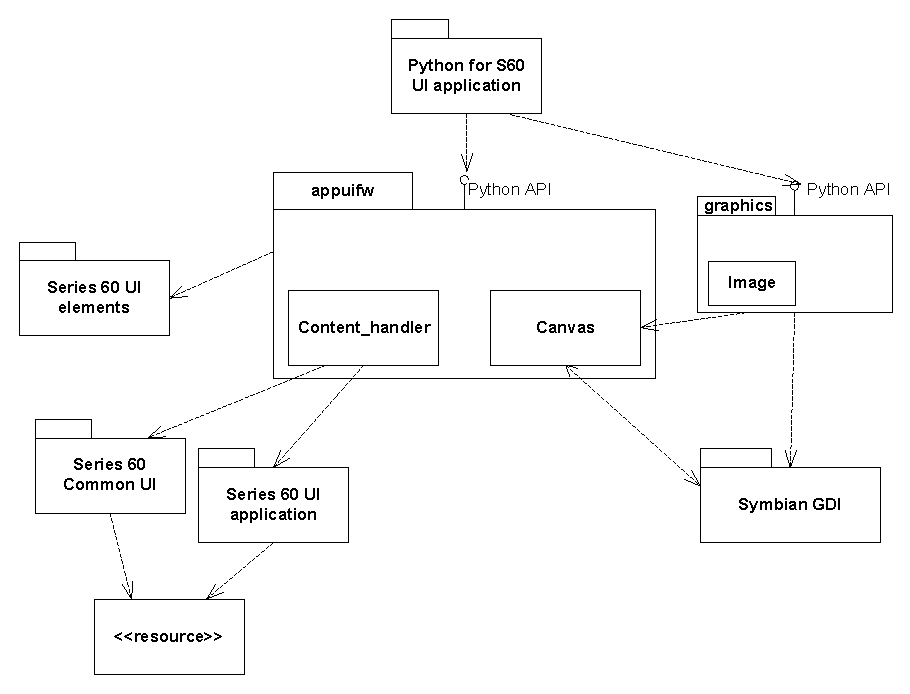
\includegraphics[width=\textwidth]{ui-overview}
\caption{Python for S60 UI environment overview}
\label{fig:ui-overview}
\end{figure}

\subsection{Basics of appuifw Module}
\label{subsec:basics}
Figure \ref{fig:normal-uilayout} shows the layout of a S60 application 
UI in the normal screen mode and a summary of how it relates to the services 
available at the \module{appuifw} API. For alternative layouts, see 
Figure \ref{fig:alternate-uilayouts}.

\begin{figure}
\centering
%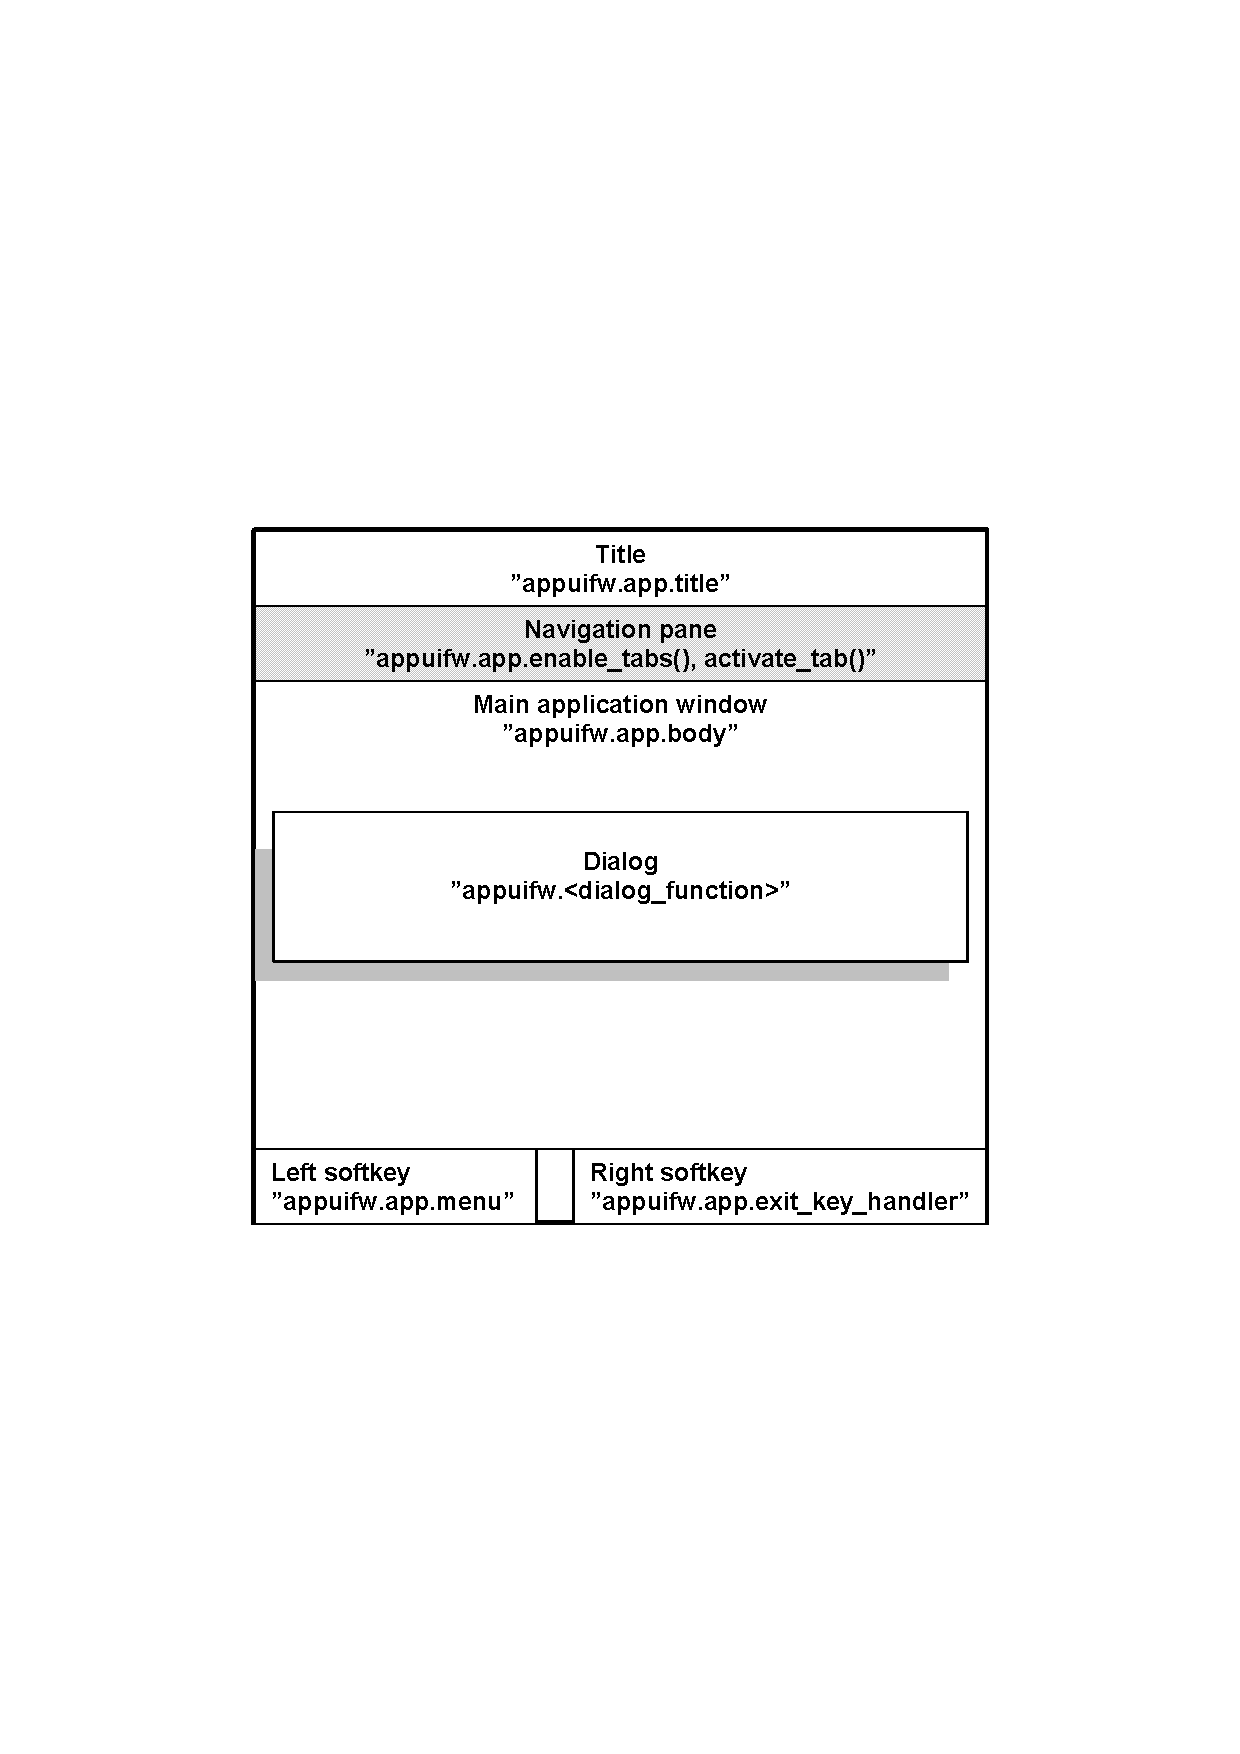
\includegraphics[width=0.7\textwidth]{screen-parts}
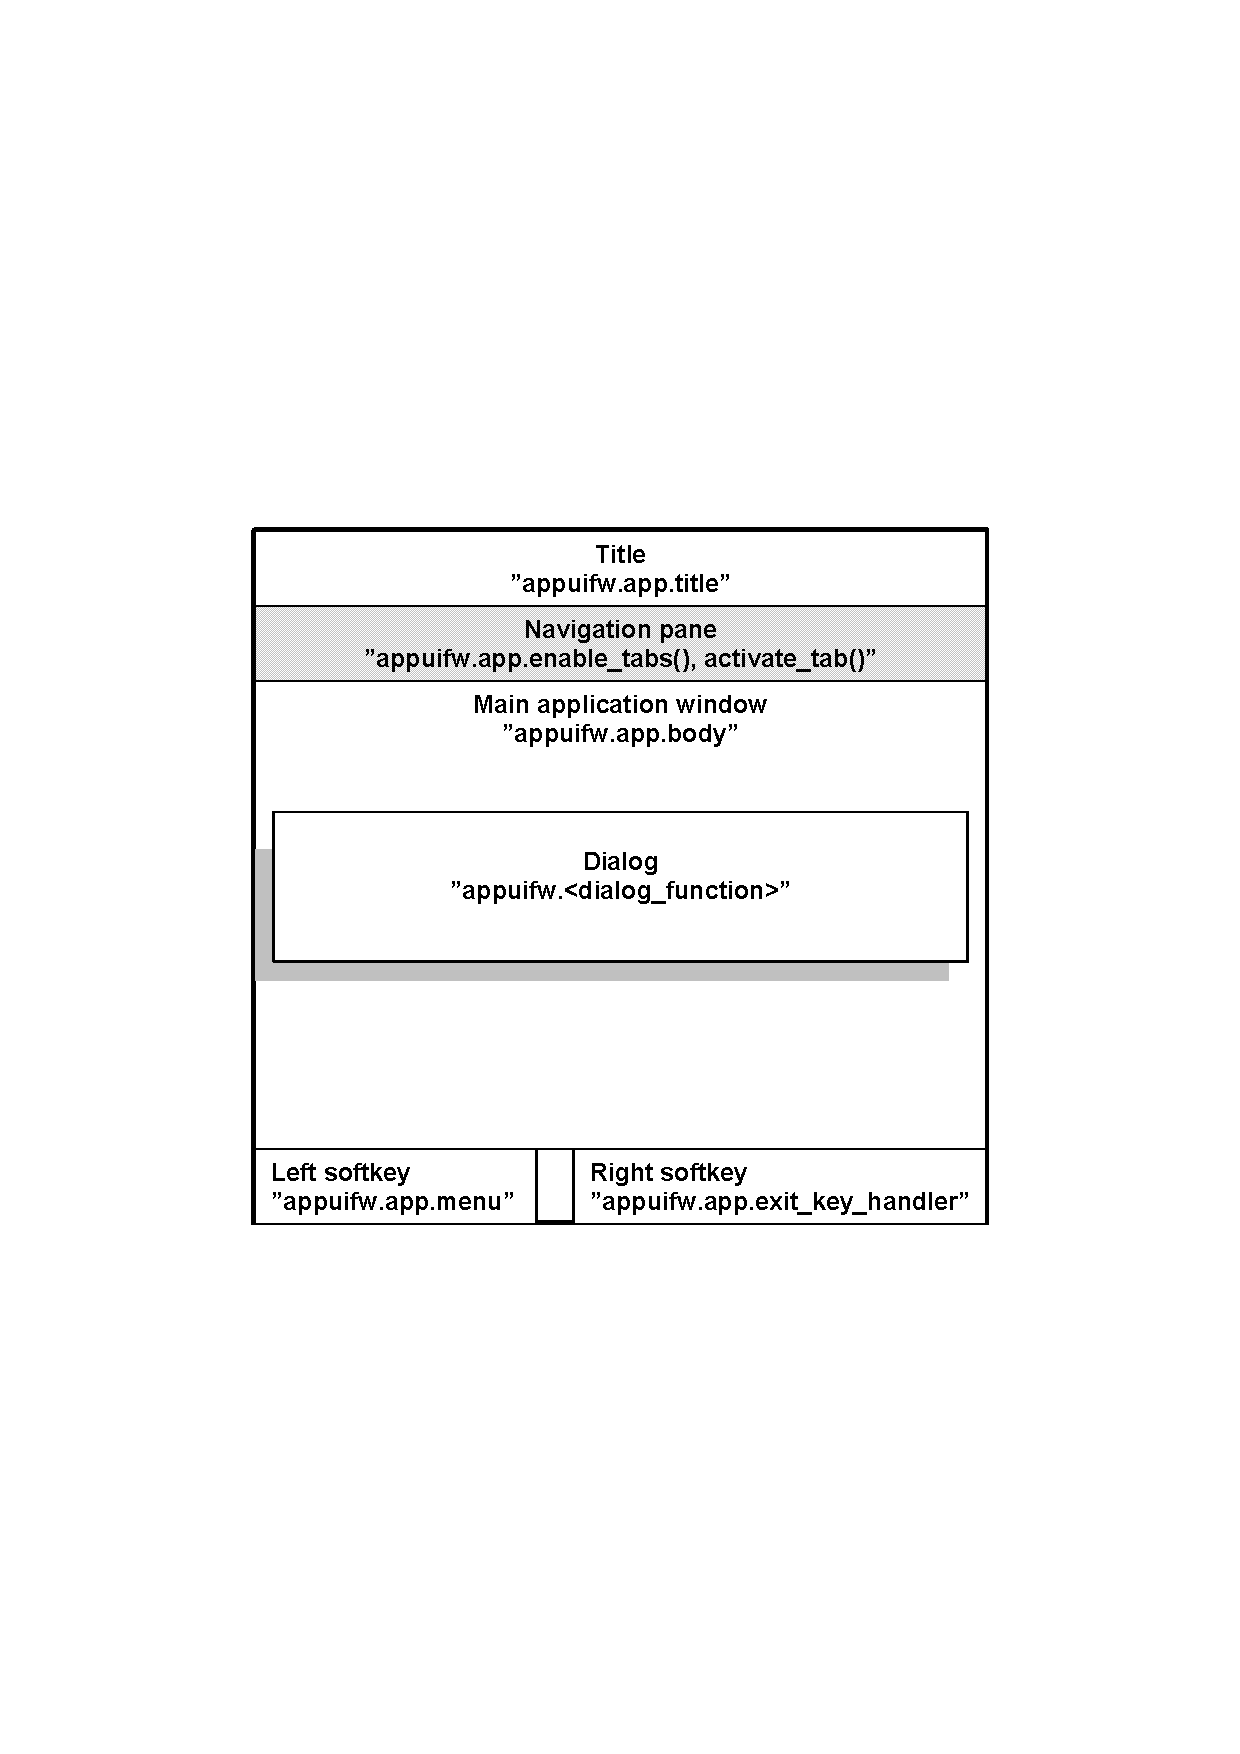
\includegraphics{screen-parts}
\caption{The different parts of the screen when using the 'normal' layout}
\label{fig:normal-uilayout}
\end{figure}

\begin{figure}
\centering
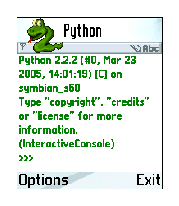
\includegraphics[width=\screenwidth]{layout-normal}
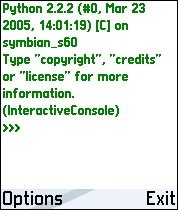
\includegraphics[width=\screenwidth]{layout-large}
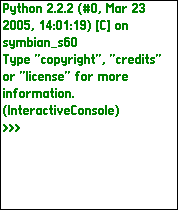
\includegraphics[width=\screenwidth]{layout-full}
\caption{UI layouts. left: 'normal', middle: 'large', right: 'full'}
\label{fig:alternate-uilayouts}
\end{figure}

The main application window may be set up to be occupied by a UI control.

A multi-view application can show the different views as tabs in the 
navigation pane and react as the users navigate between tabs. 

Dialogs always take precedence over the usual UI controls and appear on top 
of them.

UI controls are implemented as Python types. These types are available:

\begin{itemize}
\item \class{Text}
\item \class{Listbox}
\item \class{Canvas}
\end{itemize}
UI controls appear on the screen as soon as an instance of the corresponding 
Python type is set to the body field (\var{app.body}) of the current application UI.

\class{Form} is a versatile dialog implemented as a type.

The \class{Content_handler} type facilitates interfacing to other UI
applications and common high-level UI components. It is based on the
notion that designated handlers can reduce UI application interaction
to operations on MIME-type content.

The following dialogs are implemented as functions:

\begin{itemize}
\item \function{note}
\item \function{query}
\item \function{multi_query}
\item \function{selection_list}
\item \function{multi_selection_list}
\item \function{popup_menu}
\end{itemize}
A dialog becomes visible as soon as the corresponding Python function has 
been called. The function returns with the eventual user input or 
information on the cancellation of the dialog. \class{Form} is an 
exception; it is shown when its \method{execute} method is called.

\subsection{Softkeys}
\label{subsec:softkeys}
The softkeys are managed by the underlying S60 Platform. When no
dialog is visible, the right softkey is bound to application exit and
the left one represents an Options menu. Python for S60 offers
an interface for manipulating the menu and for binding the Exit key to
a Python-callable object (see Section \ref{subsec:application}). 

The native code that implements a dialog also manages the softkeys of the 
dialog, typically OK and Cancel. When the user input needs to be validated 
before accepting it and dismissing the dialog, it is best to use 
\class{Form}.

\subsection{Module Level Functions}
\label{subsec:module}
The following free functions - functions that do not belong to any class 
- are defined in the \module{appuifw} module:

\begin{funcdesc}{available_fonts}{}
Returns a list (Unicode) of all fonts available in the device.
\end{funcdesc}

\begin{funcdesc}{query}{label, type\optional{, initial_value}}
Performs a query with a single-field dialog. The prompt is set to 
\var{label}, and the type of the dialog is defined by \var{type}. The 
value of \var{type} can be any of the following strings:

\begin{itemize}
\item \code{'text'}
\item \code{'code'}
\item \code{'number'}
\item \code{'date'}
\item \code{'time'}
\item \code{'query'}
\item \code{'float'}
\end{itemize}

The type of the optional \var{initial_value} parameter and the 
returned input depend on the value of \var{type}:

\begin{itemize}
\item For text fields, (\code{'text'}, \code{'code'}) it is Unicode
\item For number fields, it is numeric
\item For date fields, it is seconds since epoch rounded down to the nearest local midnight
\end{itemize}

A simple confirmation query and time query take no initial value and return 
\code{True/None} and seconds since local midnight, correspondingly. All 
queries return \code{None} if the users cancel the dialog. 

For \code{'float'} query the \var{initial_value} setting has no 
effect.
\end{funcdesc}


\begin{funcdesc}{multi_query}{label_1, label_2}
A two-field text (Unicode) input dialog. Returns the inputted values
as a 2-tuple. Returns \code{None} if the users cancel the dialog.
\end{funcdesc}

\begin{funcdesc}{note}{text\optional{, type\optional{, global}}}
Displays a note dialog of the chosen type with \var{text} 
(Unicode). The default value for \var{type} is \code{'info'}, which is 
automatically used if \var{type} is not set. \var{type} can be one of 
the following strings: \code{'error'}, \code{'info'}, or 
\code{'conf'}. 

If \var{global} (integer) is any other value than zero a global note is 
displayed. A global note is displayed even if the Python application calling 
this function is in background. The same set of \var{type}s is supported as in 
standard note.
\end{funcdesc}

\begin{funcdesc}{popup_menu}{list\optional{, label}}
A pop-up menu style dialog. \var{list} representing the menu 
contents can be a list of Unicode strings or a list of Unicode string pairs 
(tuples). The resulting dialog list is then a single-style or a double-style 
list. A single-style list is shown in full; whereas a double-style list 
shows the items one at a time. Returns \code{None} if the user cancels the 
operation.
\end{funcdesc}

\begin{funcdesc}{selection_list}{choices\optional{, search_field=0}}
Executes a dialog that allows the users to select a list item and
returns the \var{index} of the chosen item, or \code{None} if the
selection is cancelled by the users. \var{choices} is a list of
Unicode strings.
\var{search_field} is \code{0} (disabled) by default and is optional. Setting it to \code{1} enables a search field (find pane) that facilitates searching for items in long lists. If enabled, the search field appears after you press a letter key.
\end{funcdesc}

\begin{funcdesc}{multi_selection_list}{choices\optional{, style='checkbox', search_field=0}}
  Executes a dialog that allows the users to select multiple list
  items.  Returns a tuple of indexes (a pair of Unicode strings) of
  the chosen items, or empty tuple if the selection is cancelled by
  the users. \var{choices} is a list of Unicode strings.  \var{style}
  is an optional string; the default value being \code{'checkbox'}.
  If \code{'checkbox'} is given, the list will be a checkbox list,
  where empty checkboxes indicate what items can be marked. The other
  possible value that can be set for \var{style} is
  \code{'checkmark'}. If \code{'checkmark'} is given, the list will be
  a markable list, which lists items but does not indicate
  specifically that items can be selected. To select items on a
  markable list, use the Navigation key to browse the list and the
  Edit key to select an item. For example views on checkbox and
  markable lists, see
  \figurename~\ref{fig:checkbox-and-markable-list}.
  \var{search_field} is \code{0} (disabled) by default and is
  optional. Setting it to \code{1} enables a search field (find pane)
  that facilitates searching for items in long lists. If enabled, the
  search field is always visible with checkbox lists; with markable
  lists it appears by pressing a letter key.

Example:
\begin{verbatim}
tuple = appuifw.multi_selection_list(L, style='checkmark', search_field=1)
\end{verbatim}
\end{funcdesc}

\begin{figure}[htbp]
\centering
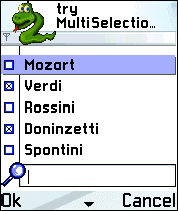
\includegraphics[width=\screenwidth]{checkbox-list}
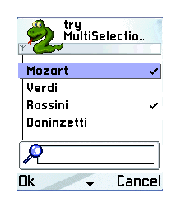
\includegraphics[width=\screenwidth]{markable-list}
\caption{Examples of a checkbox list (left) and a markable list (right)}
\label{fig:checkbox-and-markable-list}
\end{figure}

\subsection{Application Type}
\label{subsec:application}
A single implicit instance of this type always exists when \module{appuifw} 
module is present and can be referred to with the name \code{app}. New 
instances cannot be created by a Python program.

\begin{classdesc*}{Application}
Instances of \class{Application} type have the following attributes:

\begin{memberdesc}[Application]{body}
The UI control that is visible in the application's main window. Currently 
either \class{Text}, a \class{Listbox} object, \class{Canvas}, or 
\code{None}.
\end{memberdesc}

\begin{memberdesc}[Application]{exit_key_handler}
A callable object that is called when the user presses the Exit softkey. 
Setting \member{exit_key_handler} to \code{None} sets it back to the 
default value.
\end{memberdesc}

\begin{memberdesc}[Application]{menu}
This is a list of the following kinds of items:
\begin{itemize}
\item \code{(title, callback)} which creates a regular menu item
\item \code{(title, ((title, callback)\optional{...}))} which creates a submenu
\end{itemize}

\var{title} (Unicode) is the name of the item and \var{callback} the associated callable object. 
The maximum allowed number of items in a menu, or items in a submenu,
or submenus in a menu is 30.

Example:
\begin{verbatim}
appuifw.app.menu = [(u"Item 1", item1),
                    (u"Submenu 1", 
                        ((u"Subitem 1", subitem1),
                         (u"Subitem 2", subitem2)))]
\end{verbatim}
\end{memberdesc}

\begin{memberdesc}[Application]{screen}
The screen area used by an application. See \figurename~\ref{fig:alternate-uilayouts} for
example screens. The appearance of the application on the screen can
be affected by setting one of the following values: \code{'normal'},
\code{'large'}, and \code{'full'}.

Examples:
\begin{verbatim}
appuifw.app.screen='normal' # (a normal screen with title pane and softkeys)
appuifw.app.screen='large'  # (only softkeys visible)
appuifw.app.screen='full'   # (a full screen)
\end{verbatim}
\end{memberdesc}

\begin{memberdesc}[Application]{title}
The title the application that is visible in the application's title
pane. Must be Unicode.
\end{memberdesc}

\begin{memberdesc}[Application]{focus}
A callable object that is called with integer as parameter (0 = focus lost, 
1 = focus regained) when the application receives focus or it is switched to 
background. Focus is received e.g. when the application is switched from 
background to foreground or when the focus is regained from screensaver. 
Similarly when the screensaver is displayed, focus is lost.

Examples:
\begin{verbatim}
>>> import appuifw
>>> def cb(fg):
...   if(fg):
...     print "foreground"
...   else:
...     print "background"
...
>>> appuifw.app.focus=cb
>>> # switch to background, following text is printed from callback:
>>> background
>>> # switch to foreground, following text is printed from callback:
>>> foreground
\end{verbatim}

\begin{notice}
An improper callback can cause adverse effects. If you, for example,
define a callback which takes no parameters you will receive
never-ending \exception{TypeError} exceptions on the Nokia 6600.
\end{notice}

\end{memberdesc}

\begin{memberdesc}[Application]{orientation}
Available only for S60 3rdEd. 
The orientation of the application. The orientation of the application can be 
one of the following values: \code{'automatic'} (this is the default value), 
\code{'portrait'} or \code{'landscape'}.
\end{memberdesc}

Instances of \class{Application} type have the following methods:

\begin{methoddesc}[Application]{activate_tab}{index}
Activates the tab \var{index} counting from zero.
\end{methoddesc}

\begin{methoddesc}[Application]{full_name}{}
Returns the full name, in Unicode, of the native application in whose 
context the current Python interpreter session runs.
\end{methoddesc}

\begin{methoddesc}[Application]{uid}{}
Returns the UID, in Unicode, of the native application in whose 
context the current Python interpreter session runs.
\end{methoddesc}

\begin{methoddesc}[Application]{set_exit}{}
Requests a graceful exit from the application as soon as the current script 
execution returns.
\end{methoddesc}

\begin{methoddesc}[Application]{set_tabs}{tab_texts\optional{,callback=None}}
Sets tabs with given names on them in the navigation bar; 
\var{tab_texts} is a list of Unicode strings. When the users 
navigate between tabs, \var{callback} gets called with the index 
of the active tab as an argument. Tabs can be disabled by giving an empty or 
one-item \var{tab_texts} list.
\end{methoddesc}


\begin{methoddesc}[Application]{layout}{layout_id}

\begin{notice}[note]
Available from S60 2ndEd FP3 onwards (inclusive).
\end{notice}

Returns as a tuple the size and the position of the requested \code{layout_id}. 
The logical layouts are outlined partly in Figure \ref{fig:normal-uilayout}. The 
position is given from the top left corner. The \code{layout_id} can be one of 
the constants defined in module \module{appuifw}\footnote{Descriptions of the 
values are from the S60 SDK documentation \cite{S60Doc}.}:

\begin{datadesc}{EScreen} 
Screen.  
\end{datadesc}

\begin{datadesc}{EApplicationWindow} 
 Window that fills the entire screen.
\end{datadesc}

\begin{datadesc}{EStatusPane} 
Indicates common components for most of the applications.  
\end{datadesc}

\begin{datadesc}{EMainPane} 
The application main pane is used in all the applications.  
\end{datadesc}

\begin{datadesc}{EControlPane} 
Control pane.
\end{datadesc}

\begin{datadesc}{ESignalPane} 
The signal pane is used to indicate signal strength.  
\end{datadesc}

\begin{datadesc}{EContextPane} 
The context pane is used to indicate an active application.
\end{datadesc}

\begin{datadesc}{ETitlePane} 
Used to indicate the subject or the name of the main pane content. 
\end{datadesc}

\begin{datadesc}{EBatteryPane} 
The battery pane is used to indicate battery strength.  
\end{datadesc}

\begin{datadesc}{EUniversalIndicatorPane} 
The universal indicator pane is used to indicate items that require the user's 
attention while browsing applications. 
\end{datadesc}

\begin{datadesc}{ENaviPane} 
The navi pane is used to indicate navigation within an application, to provide 
context sensitive information to the user while entering or editing data, or to 
show additional information.  
\end{datadesc}

\begin{datadesc}{EFindPane} 
A fixed find pane is used with lists instead of the find pop-up window.  
\end{datadesc}

\begin{datadesc}{EWallpaperPane} 
Wallpaper pane.  
\end{datadesc}

\begin{datadesc}{EIndicatorPane} 
The universal indicator pane is used to indicate items that require the user's 
attention while browsing applications.  
\end{datadesc}

\begin{datadesc}{EAColumn} 
Used generally to display small sized graphics or heading texts.  
\end{datadesc}

\begin{datadesc}{EBColumn} 
Used generally to display large sized icons or heading texts.  
\end{datadesc}

\begin{datadesc}{ECColumn} 
Used generally to display data entered by the user. Overlaps with the D column. 
\end{datadesc}

\begin{datadesc}{EDColumn} 
Used generally to display additional icons. Overlaps with the C column. 
\end{datadesc}

\begin{datadesc}{EStaconTop} 
Top part of status and control panes in landscape layout.  
\end{datadesc}

\begin{datadesc}{EStaconBottom} 
Bottom part of status and control panes in landscape layout.  
\end{datadesc}

\begin{datadesc}{EStatusPaneBottom} 
Bottom part of status pane in landscape layout.  
\end{datadesc}

\begin{datadesc}{EControlPaneBottom} 
Bottom part of control pane in landscape layout.  
\end{datadesc}

\begin{datadesc}{EControlPaneTop} 
Top part of control pane in landscape layout.  
\end{datadesc}

\begin{datadesc}{EStatusPaneTop} 
Top part of status pane in landscape layout.
\end{datadesc}

Example:
\begin{verbatim}
>>> import appuifw
>>> appuifw.app.layout(appuifw.EMainPane)
((176, 144), (0, 44))
>>> # size and position (x, y) of the main pane in Nokia N70
\end{verbatim}

\end{methoddesc}

\end{classdesc*}

\subsection{Form Type}
\label{subsec:form}
\class{Form} implements a dynamically configurable, editable multi-field 
dialog. \class{Form} caters for advanced dialog use cases with requirements 
such as free selectability of the combination of fields, possibility of 
validating the user input, and automatically producing the contents of some 
dialog fields before allowing the closing of the dialog. 

\begin{classdesc}{Form}{fields\optional{, flags=0}}
Creates a \class{Form} instance.
\var{fields} is a list of \emph{field descriptors}: \code{(label, type\optional{, value})} where

\var{label} is a Unicode string

\var{type} is one of the following strings: 
\code{'text'}, \code{'number'}, \code{'date'}, \code{'time'}, \code{'combo'}
or \code{'float'}

\var{value}, depending on \var{type}: Unicode string, numeric, float (seconds 
since Unix epoch rounded down to the nearest local midnight), float (seconds 
since local midnight), \code{([choice_label ...], index)} of float. For 
\code{'float'} \var{type} the initial value setting might not be shown in the 
UI.
\end{classdesc}

\class{Form} can also be configured and populated after construction. The 
configuration flags are visible as an attribute. \class{Form} implements 
the list protocol that can be used for setting the form fields, as well as 
obtaining their values after the dialog has been executed.

Instances of \class{Form} type have the following attributes:

\begin{memberdesc}[Form]{flags}
This attribute holds the values of the various configuration flags. 
Currently supported flags are:

\begin{datadesc}{FFormEditModeOnly}
When this flag is set, the form remains in edit mode while \method{execute} 
runs.
\end{datadesc}

\begin{datadesc}{FFormViewModeOnly}
When this flag is set, the form cannot be edited at all.
\end{datadesc}

\begin{datadesc}{FFormAutoLabelEdit}
This flag enables support for allowing the end-users to edit the labels of 
the form fields.
\end{datadesc}

\begin{datadesc}{FFormAutoFormEdit}
This flag enables automatic support for allowing the end-users to add and 
delete the form fields. Note that this is an experimental feature and is not 
guaranteed to work with all SDK versions.
\end{datadesc}

\begin{datadesc}{FFormDoubleSpaced}
When this flag is set, double-spaced layout is applied when the form is 
executed: one field takes two lines, as the label and the value field are on 
different lines.
\end{datadesc}
\end{memberdesc}

\begin{memberdesc}[Form]{menu}
A list of \code{(title, callback)} pairs, where 
each pair describes an item in the form's menu bar that is active while the 
dialog is being executed. \var{title} (Unicode) is the name of 
the item and \var{callback} the associated callable object.
\end{memberdesc}

\begin{memberdesc}[Form]{save_hook}
This attribute can be set to a callable object that receives one argument 
and returns a Boolean value. It gets called every time the users want to 
save the contents of an executing \class{Form} dialog. A candidate list for 
new form content - a list representing the currently visible state of the 
UI - is given as an argument. The list can be modified by 
\member{save_hook}. If \member{save_hook} returns \code{True}, the 
candidate list is set as the new contents of the form. Otherwise, the form 
UI is reset to reflect the field list contained in \class{Form} object.
\end{memberdesc}

Instances of \class{Form} type have the following methods:

\begin{methoddesc}[Form]{execute}{}
Executes the dialog by making it visible on the UI.
\end{methoddesc}

\begin{methoddesc}[Form]{insert}{index, field_descriptor}
Inserts the field descriptor into the \class{Form} before the given \var{index}.
\end{methoddesc}

\begin{methoddesc}[Form]{pop}{}
Removes the last field descriptor from the \class{Form} and returns it.
\end{methoddesc}

\begin{methoddesc}[Form]{length}{}the number of field descriptors in the form.
\end{methoddesc}

The subscript notation \code{f[i]} can be used to access or modify the
i-th element of the form \code{f}. Same limitations as discussed above
in the context of the flag \constant{FFormAutoFormEdit} apply to
modifying a form while it is executing. The ability to change the
schema of a form while it is executing is an experimental feature.

\subsection{Text Type}
\label{subsec:mylabel5}
\class{Text} is a text editor UI control. For examples on the options 
available with \class{Text}, see Figure \ref{fig:text-styles}.

\begin{figure}[htbp]
\centering
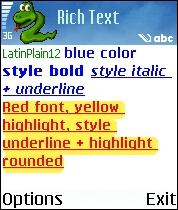
\includegraphics[width=\screenwidth]{text-styles-1}
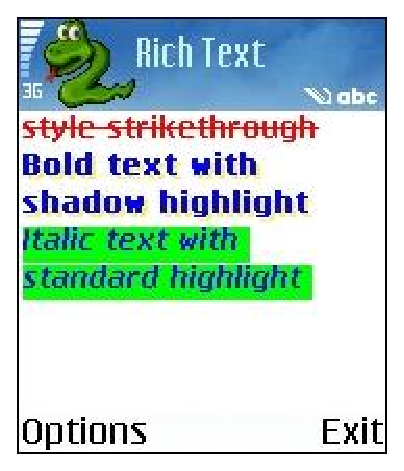
\includegraphics[width=\screenwidth]{text-styles-2}
\caption{Examples of the options available for Text type}
\label{fig:text-styles}
\end{figure}

Instances of \class{Text} type have the following attributes:

\begin{memberdesc}[Text]{color}
The color of the text. \code{color} supports the same color representation 
models as the \module{graphics} module. For the supported color 
representation models, see Section \ref{sec:graphics}.
\end{memberdesc}

\begin{memberdesc}[Text]{focus}
A Boolean attribute that indicates the focus state of the control. Editor 
control also takes the ownership of the navigation bar, and this feature is 
needed to enable the usage of this control in applications that use the 
navigation bar - for example, navigation tabs.
\end{memberdesc}

\begin{memberdesc}[Text]{font} 
The font of the text. There are two possible ways to set this attribute:

\begin{itemize}

\item Using a supported Unicode font, for example \code{u"Latin12"}. Trying to set a font which is not supported by the device has no effect. A list of supported fonts can be retrieved by using \function{appuifw.available_fonts}.

Example, setting font:
\begin{verbatim}
t = appuifw.Text()
t.font = u"albi17b" # sets font to Albi 17 bold
t.font = u"LatinPlain12" # sets font to Latin Plain 12
\end{verbatim}
\item Using one of the default device fonts that are associated with the following labels (plain strings):
\code{'annotation', 'title', 'legend', 'symbol', 'dense', 'normal'}
Example, setting font: 
\begin{verbatim}
t.font = "title" # sets font to the one used in titles
\end{verbatim}

Example, checking the currently set font: 
\begin{verbatim}
unicodeFont = t.font
\end{verbatim}
\end{itemize}

The attribute value retrieved is always a Unicode string. If the font has 
been set with a label, for example, \code{'title'}, the attribute will 
retrieve the font associated with that label. 
\end{memberdesc}

\begin{memberdesc}[Text]{highlight_color}
The highlight color of the text. \code{highlight_color} supports the 
same color representation models as the \module{graphics} module. For the 
supported color representation models, see Section \ref{sec:graphics}.
\end{memberdesc}

\begin{memberdesc}[Text]{style}
The style of the text. The flags for this attribute are defined in the 
\module{appuifw} module. These flags can be combined by using the binary 
operator \code{|}. The flags can be divided into two types: text style 
and text highlight. Text style flags can be freely combined with each other. 
However, one or more text style flags can be combined with only one text 
highlight flag. The flags are:

Text style:

\begin{datadesc}{STYLE_BOLD} 
Enables bold text.
\end{datadesc}

\begin{datadesc}{STYLE_UNDERLINE}
Enables underlined text.
\end{datadesc}

\begin{datadesc}{STYLE_ITALIC} 
Enables italic text.
\end{datadesc}

\begin{datadesc}{STYLE_STRIKETHROUGH } 
Enables strikethrough.
\end{datadesc}

Text highlight:

\begin{datadesc}{HIGHLIGHT_STANDARD}
Enables standard highlight.
\end{datadesc}

\begin{datadesc}{HIGHLIGHT_ROUNDED}
Enables rounded highlight.
\end{datadesc}

\begin{datadesc}{HIGHLIGHT_SHADOW}
Enables shadow highlight.
\end{datadesc}

Only one highlight is allowed to be used at once. Therefore, it is possible 
to combine only one highlight with one or more text styles.

Examples:
\begin{verbatim}
t = appuifw.Text()

# These and other similar values and combinations are valid:
t.style = appuifw.STYLE_BOLD
t.style = appuifw.STYLE_UNDERLINE
t.style = appuifw.STYLE_ITALIC
t.style = appuifw.STYLE_STRIKETHROUGH
t.style = (appuifw.STYLE_BOLD|
	   appuifw.STYLE_ITALIC|
	   appuifw.STYLE_UNDERLINE)

# These values are valid:
t.style = appuifw.HIGHLIGHT_STANDARD
t.style = appuifw.HIGHLIGHT_ROUNDED
t.style = appuifw.HIGHLIGHT_SHADOW

# This combination is NOT valid:
# Invalid code, do not try!
t.style = (appuifw.HIGHLIGHT_SHADOW|appuifw.HIGHLIGHT_ROUNDED)
\end{verbatim}
\end{memberdesc}

Instances of \class{Text} type have the following methods:

\begin{methoddesc}[Text]{add}{text}
Inserts the Unicode string \var{text} to the current cursor position.
\end{methoddesc}

\begin{methoddesc}[Text]{bind}{event_code, callback}
Binds the callable Python object \var{callback} to event
\var{event_code}. The key codes are defined in 
the \module{key_codes} library module. The call 
\code{bind(event_code, None)} clears an 
existing binding. In the current implementation the event is always
passed also to the underlying native UI control.
\end{methoddesc}

\begin{methoddesc}[Text]{clear}{}
Clears the editor.
\end{methoddesc}

\begin{methoddesc}[Text]{delete}{\optional{pos=0, length=len()}}
Deletes \var{length} characters of the text held by the editor control, 
starting from the position \var{pos}.
\end{methoddesc}

\begin{methoddesc}[Text]{get_pos}{}
Returns the current cursor position.
\end{methoddesc}

\begin{methoddesc}[Text]{len}{}
Returns the length of the text string held by the editor control.
\end{methoddesc}

\begin{methoddesc}[Text]{get}{\optional{pos=0, length=len()}}
Retrieves \code{length} characters of the text held by the editor control, 
starting from the position \var{pos}.
\end{methoddesc}

\begin{methoddesc}[Text]{set}{text}
Sets the text content of the editor control to Unicode string 
\var{text}.
\end{methoddesc}

\begin{methoddesc}[Text]{set_pos}{cursor_pos}
Sets the cursor to \var{cursor_pos}.
\end{methoddesc}

\subsection{Listbox Type}
\label{subsec:listbox}

\begin{figure}[htbp]
\centering
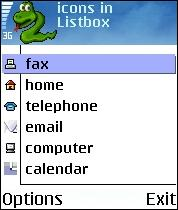
\includegraphics[width=\screenwidth]{listbox-with-icons}
\caption{Listbox with icons}
\label{fig:listbox-with-icons}
\end{figure}

An instance of this UI control type is visible as a listbox, also known as a 
list in Symbian, that can be configured to be a single-line item or a 
double-item listbox. Figure \ref{fig:listbox-with-icons} shows a single-line 
item Listbox with icons. For more information on the MBM and MIF formats, 
see Section \ref{subsec:icon}.

\begin{classdesc}{Listbox}{list, callback}
Creates a \class{Listbox} instance. A callable object 
\var{callback} gets called when a listbox selection has been 
made. \code{list} defines the content of the listbox and can be one of the 
following:

\begin{itemize}
\item A normal (single-line item) listbox: a list of Unicode strings, for example \code{[unicode_string item1, unicode_string item2]}
\item A double-item listbox: a two-element tuple of Unicode strings , for example \code{[(unicode_string item1, unicode_string item1description), (unicode_string item2, unicode_string item2description)]}
\item A normal (single-line item) listbox with graphics: a two-element tuple consisting of a Unicode string and an \class{Icon} object, for example \code{[(unicode_string item1, icon1), (unicode_string item2, icon2)]}.
\item A double-item listbox with graphics: a three-element tuple consisting of two Unicode strings and one \class{Icon} object, for example \code{[(unicode_string item1, unicode_string item1description, icon1), (unicode_string item2, unicode_string item2description, icon2)]}
\end{itemize}

Example: To produce a normal (single-line item) listbox with graphics:
\begin{verbatim}
icon1 = appuifw.Icon(u"z:\\system\\data\\avkon.mbm", 28, 29)
icon2 = appuifw.Icon(u"z:\\system\\data\\avkon.mbm", 40, 41)
entries = [(u"Signal", icon1),
           (u"Battery", icon2)]
lb = appuifw.Listbox(entries, lbox_observe)
\end{verbatim}
\end{classdesc}

Instances of \class{Listbox} type have the following methods:

\begin{methoddesc}[Listbox]{bind}{event_code, callback}
Binds the callable Python object \var{callback} to event 
\var{event_code}. The key codes are defined in 
the \module{key_codes} library module. The call
\code{bind(event_code, None)} clears an 
existing binding. In the current implementation the event is always passed 
also to the underlying native UI control.
\end{methoddesc}

\begin{methoddesc}[Listbox]{current}{}
Returns the currently selected item's index in the \class{Listbox}.
\end{methoddesc}

\begin{methoddesc}[Listbox]{set_list}{list\optional{, current}}
Sets the \class{Listbox} content to a list of Unicode strings or a
list of tuples of Unicode strings. The accepted structures of \var{list} are the
same as in the \class{Listbox} constructor. The optional argument \var{current} is the index of the focused list item.
\end{methoddesc}

\subsection{Icon Type}
\label{subsec:icon}
An instance of \class{Icon} type encapsulates an icon to be used together 
with a \class{Listbox} instance. Note that currently \class{Icon} can only 
be used with \class{Listbox} (see Section \ref{subsec:listbox}).

MBM is the native Symbian OS format used for pictures. It is a
compressed file format where the files can contain several bitmaps and
can be referred to by a number. An \code{.mbg} file is the header file
usually associated with an \code{.mbm} file, which includes symbolic
definitions for each bitmap in the file. For example, an
\file{avkon.mbm} file has an associated index file called
\file{avkon.mbg}, which is included in S60 SDKs. For more information
on the MBM format and the bitmap converter tool, see \cite{S60Doc} and
search the topics with the key term "How to provide Icons"; this topic
also points you to the Bitmap Converter tool that can be used for
converting bitmaps into the MBM format.

S60 2$^{nd}$ Edition FP3 introduces a new format for icons called 
Multi-Image File (MIF). This format is very similar to the MBM format and 
also contains several compressed files. The files to be compressed should be 
in Scalable Vector Graphics Tiny (SVG-T) format. For more information on the 
SVG format, see Scalable Vector Graphics (SVG) 1.1 Specification 
[10].

\begin{classdesc}{Icon}{filename, bitmap, bitmapMask}
Creates an icon. \var{filename} is a Unicode file name and must 
include the whole path. Note that MBM and MIF (MIF only in S60 2nd 
Edition FP3) are the only file formats supported. \var{bitmap} 
and \var{bitmapMask} are integers that represent the index of 
the icon and icon mask inside that file respectively.
\end{classdesc}

Example: The following builds an icon with the standard signal symbol:
\begin{verbatim}
icon = appuifw.Icon(u"z:\\system\\data\\avkon.mbm", 28, 29)
\end{verbatim}

\subsection{Content_handler Type}
\label{subsec:content}

An instance of \class{Content_handler} handles data content by its MIME 
type.

\begin{classdesc}{Content_handler}{\optional{callback}}
Creates a \class{Content_handler} instance. A Content_handler handles
data content by its MIME type. The optional
\var{callback} is called when the embedded handler application 
started with the \method{open} method finishes. 
\end{classdesc}

Instances of \class{Content_handler} type have the following methods:

\begin{methoddesc}[Content_handler]{open}{filename}
Opens the file \var{filename} (Unicode) in its handler 
application if one has been registered for the particular MIME type. The 
handler application is embedded in the caller's thread. The call to this 
function returns immediately. When the handler application finishes, the 
\var{callback} that was given to the \class{Content_handler} 
constructor is called.
\end{methoddesc}

\begin{methoddesc}[Content_handler]{open_standalone}{filename}
Opens the file \var{filename} (Unicode) in its handler 
application if one has been registered for the particular MIME type. The 
handler application is started in its own process. The call to this function 
returns immediately. Note that \var{callback} is not called for 
applications started with this method.
\end{methoddesc}

\subsection{Canvas Type}
\label{subsec:canvas}
\class{Canvas} is a UI control that provides a drawable area on the screen 
and support for handling raw key events. \class{Canvas} supports the 
standard drawing methods that are documented in Section \ref{sec:graphics}.

\begin{classdesc}{Canvas}{\optional{redraw_callback=None, event_callback=None,
                                  resize_callback=None}}
Constructs a \class{Canvas}. The optional parameters are callbacks
that are called when specific events occur. 

\note{Watch out for cyclic
references here. For example, if the callbacks are methods of an
object that holds a reference to the \class{Canvas}, a reference cycle
is formed that must be broken at cleanup time or the
\class{Canvas} will not be freed.}

\var{redraw_callback} is called whenever a part of the \class{Canvas} 
has been obscured by something, is then revealed, and needs to be
redrawn. This can typically happen, for example, when the user
switches away from the Python application and back again, or after
displaying a pop-up menu. The callback takes as its argument a
four-element tuple that contains the top-left and the bottom-right
corner of the area that needs to be redrawn. In many cases redrawing
the whole
\class{Canvas} is a reasonable option. 

\var{event_callback} is called whenever a raw key event is received.
There are three kinds of key events: \code{EEventKeyDown},
\code{EEventKey}, and \code{EEventKeyUp}. When a user presses a key 
down, events \code{EEventKeyDown} and \code{EEventKey} are generated. 
When the key is released, an \code{EEventKeyUp} event is generated.

The argument to the \var{event_callback} is a dictionary that contains 
the following data for key events:

\begin{itemize}
\item \code{'type'}: one of \code{EEventKeyDown}, \code{EEventKey}, or \code{EEventKeyUp}
\item \code{'keycode'}: the keycode of the key
\item \code{'scancode'}: the scancode of the key
\item \code{'modifiers'}: the modifiers that apply to this key event
\end{itemize}

Each key on the keyboard has one or more scancodes and zero or more keycodes 
associated with it. A scancode represents the physical key itself and a 
keycode is the result of state-related operating system defined processing 
done on the key. For keys that correspond to a symbol in the current 
character set of the phone, the keycode is equal to the code of the 
corresponding symbol in that character set. For example, if you are using 
the Nokia Wireless Keyboard (SU-8W), pressing the key A will always produce 
the scancode 65 (ASCII code for an upper case A), but the keycode 
could be either 65 or 91 (ASCII code for a lower case A) depending on 
whether or not the Shift key is pressed or Caps Lock is active. 

The \module{key_codes} module contains definitions for the keycodes and 
scancodes. See \figurename~\ref{fig:keyboard} for the codes of the most 
common keys on the phone keypad. 

Some keys are handled in a special way:

\begin{itemize}
\item A short press of the Edit key causes it to stay down, meaning that no \code{EEventKeyUp} event is sent. The event is only sent after a long press.
\item Detecting presses of the Voice tags key or the Power key is not supported.
\item If the right softkey is pressed, the \code{appuifw.app.exit_key_handler} callback is always executed.
\end{itemize}

There is no way to prevent the standard action of the Hang-up key, the Menu 
key, the Power key or the Voice tags key from taking place.

\begin{figure}
\centering
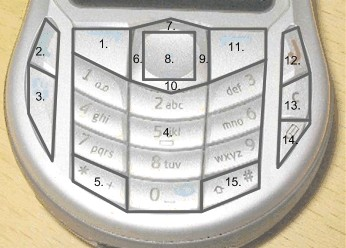
\includegraphics[width=5in]{6630keyboard}
%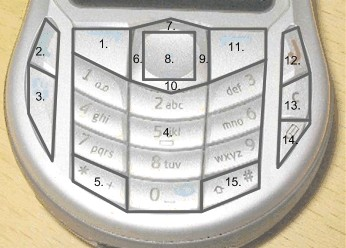
\includegraphics[width=3.60in,height=2.58in]{6630keyboard}
%\centerline{\includegraphics[width=3.60in,height=2.58in]{API_Reference_for_Python11.eps}} \par & 
\begin{tableiii}{lll}{textrm}{Key}{Keycode}{Scancode}
\lineiii{1.}{EKeyLeftSoftkey}{EScancodeLeftSoftkey}
\lineiii{2.}{EKeyYes}{EScancodeYes}
\lineiii{3.}{EKeyMenu}{EScancodeMenu}
\lineiii{4.}{EKey0...9}{EScancode0...9}
\lineiii{5.}{EKeyStar}{EScancodeStar}
\lineiii{6.}{EKeyLeftArrow}{EScancodeLeftArrow}
\lineiii{7.}{EKeyUpArrow}{EScancodeUpArrow}
\lineiii{8.}{EKeySelect}{EScancodeSelect}
\lineiii{9.}{EKeyRightArrow}{EScancodeRightArrow}
\lineiii{10.}{EKeyDownArrow}{EScancodeDownArrow}
\lineiii{11.}{EKeyRightSoftkey}{EScancodeRightSoftkey}
\lineiii{12.}{EKeyNo}{EScancodeNo}
\lineiii{13.}{EKeyBackspace}{EScancodeBackspace}
\lineiii{14.}{EKeyEdit}{EScancodeEdit}
\lineiii{15.}{EKeyHash}{EScancodeHash}
\end{tableiii}
\caption{Keycodes and scancodes for phone keys usable from Python applications}
\label{fig:keyboard}
\end{figure}

\var{resize_callback} is called when screen size is changed when the 
\class{Canvas} rect size has been changed. The callback takes as its argument a
two-element tuple that contains the new clientRect width and height. 

\end{classdesc}

Instances of \class{Canvas} type have the following attribute:

\begin{memberdesc}[Canvas]{size}
A two-element tuple that contains the current width and height of the 
\class{Canvas} as integers.
\end{memberdesc}

Instances of \class{Canvas} type have the same standard drawing methods 
that are documented in Section \ref{sec:graphics}.

% Copyright (c) 2005-2007 Nokia Corporation
%
% Licensed under the Apache License, Version 2.0 (the "License");
% you may not use this file except in compliance with the License.
% You may obtain a copy of the License at
%
%     http://www.apache.org/licenses/LICENSE-2.0
%
% Unless required by applicable law or agreed to in writing, software
% distributed under the License is distributed on an "AS IS" BASIS,
% WITHOUT WARRANTIES OR CONDITIONS OF ANY KIND, either express or implied.
% See the License for the specific language governing permissions and
% limitations under the License.

\newcommand{\notinfirsted}{
\begin{notice}
Not supported in S60 1st Edition!
\end{notice}

}

\section{\module{graphics} ---
  A graphics related services package}
\label{sec:graphics}

\declaremodule{extension}{graphics}
\platform{S60}
\modulesynopsis{A graphics related services package.}

The \module{graphics} module provides access to the graphics primitives and 
image loading, saving, resizing, and transformation capabilities provided by 
the Symbian OS. 

The module is usable from both graphical Python applications and
background Python processes. However, background processes have some
restrictions, namely that plain string symbolic font names are not
supported in background processes since background processes have no
access to the UI framework (see also Section
\ref{subsubsec:font-specs}).

For an example on using this module, see \cite{PyS60Prog}.

Functions \function{Image.open} and \function{Image.inspect} and \class{Image} 
object methods \method{load}, \method{save}, \method{resize}, and 
\method{transpose} are not available for S60 1st Edition.

\subsection{Module Level Functions}
\label{subsec:mylabel7}
The following free functions - functions that do not belong to any class 
- are defined in the \module{graphics} module:

\begin{funcdesc}{screenshot}{}
Takes a screen shot and returns the image in \class{Image} format.
\end{funcdesc}

\subsection{Image Class Static Methods}
\label{subsec:image}
The following \class{Image} class static methods are defined in the 
\module{graphics} module:

\begin{funcdesc}{Image.new}{size\optional{, mode='RGB16'}}
Creates and returns a new \class{Image} object with the given size and 
mode. \var{size} is a two-element tuple. \var{mode} specifies the 
color mode of the \class{Image} to be created. It can be one of the 
following:

\begin{itemize}
\item \code{'1'}: Black and white (1 bit per pixel)
\item \code{'L'}: 256 gray shades (8 bits per pixel)
\item \code{'RGB12'}: 4096 colors (12 bits per pixel)
\item \code{'RGB16'}: 65536 colors (16 bits per pixel)
\item \code{'RGB'}: 16.7 million colors (24 bits per pixel)
\end{itemize}
\end{funcdesc}

\begin{funcdesc}{Image.open}{filename}
\notinfirsted
Returns a new \class{Image} object (mode \code{RGB16}) that contains the 
contents of the named file. The supported file formats are JPEG and PNG. The 
file format is automatically detected based on file contents. 
\var{filename} should be a full path name.
\end{funcdesc}

\begin{funcdesc}{Image.inspect}{filename}
\notinfirsted
Examines the given file and returns a dictionary of the attributes of the 
file. At present the dictionary contains only the image size in pixels as a 
two-element tuple, indexed by key \code{'size'}. 
\var{filename} should be a full path name.
\end{funcdesc}

\subsection{Image Objects}
\label{subsec:image-objects}
An \class{Image} object encapsulates an in-memory bitmap. 

Note on asynchronous methods: Methods \method{resize}, \method{transpose}, 
\method{save}, and \method{load} have an optional callback argument. If the 
callback is not given, the method call is synchronous; when the method
returns, the operation is complete or an exception has been raised. If
the callback is given, the method calls are asynchronous. If all
parameters are valid and the operation can start, the method call will
return immediately.  The actual computation then proceeds in the
background. When it is finished, the callback is called with an error
code as the argument. If the given code is \code{0}, the operation
completed without errors, otherwise an error occurred.

It is legal to use an unfinished image as a source in a blit operation; this 
will use the image data as it is at the moment the blit is made and may thus 
show an incomplete result.

\class{Image} objects have the following methods:

\begin{methoddesc}[Image]{resize}{newsize\optional{, callback=None, keepaspect=0}}
\notinfirsted
Returns a new image that contains a resized copy of this image. If 
\var{keepaspect} is set to \code{1}, the resize will maintain the 
aspect ratio of the image, otherwise the new image will be exactly the given 
size. 

If \var{callback} is given, the operation is asynchronous, and the 
returned image will be only partially complete until \var{callback} is 
called.
\end{methoddesc}

\begin{methoddesc}[Image]{transpose}{direction\optional{, callback=None}}
\notinfirsted

Creates a new image that contains a transformed copy of this image. The 
\var{direction} parameter can be one of the following:

\begin{itemize}
\item \code{FLIP_LEFT_RIGHT}: Flips the image horizontally, exchanging left and right edges.
\item \code{FLIP_TOP_BOTTOM}: Flips the image vertically, exchanging top and bottom edges.
\item \code{ROTATE_90}: Rotates the image 90 degrees counterclockwise.
\item \code{ROTATE_180}: Rotates the image 180 degrees.
\item \code{ROTATE_270}: Rotates the image 270 degrees counterclockwise.
\end{itemize}

If \var{callback} is given, the operation is asynchronous and the 
returned image will be only partially complete until \var{callback} is 
called.
\end{methoddesc}

\begin{methoddesc}[Image]{load}{filename\optional{, callback=None}}
\notinfirsted
Replaces the contents of this \class{Image} with the contents of the named 
file, while keeping the current image mode. This \class{Image} object must 
be of the same size as the file to be loaded.

If \var{callback} is given, the operation is asynchronous and the loaded 
image will be only partially complete until \var{callback} is called. 
\var{filename} should be a full path name.
\end{methoddesc}

\begin{methoddesc}[Image]{save}{filename\optional{,callback=None, format=None, quality=75, bpp=24, compression='default'}}
\notinfirsted
Saves the image into the given file. The supported formats are JPEG and PNG. 
If \var{format} is not given or is set to \code{None}, the format is 
determined based on the file name extension: \code{'.jpg'} or 
\code{'.jpeg'} are interpreted to be in JPEG format and \code{'.png'} to 
be in PNG format. \var{filename} should be a full path name.

When saving in JPEG format, the \var{quality} argument specifies the 
quality to be used and can range from 1 to 100. 

When saving in PNG format, the \var{bpp} argument specifies how many bits 
per pixel the resulting file should have, and \var{compression} specifies 
the compression level to be used. 

Valid values for \var{bpp} are:

\begin{itemize}
\item \code{1}: Black and white, 1 bit per pixel
\item \code{8}: 256 gray shades, 8 bits per pixel
\item \code{24}: 16.7 million colors, 24 bits per pixel
\end{itemize}

Valid values for \var{compression} are:

\begin{itemize}
\item \code{'best'}: The highest possible compression ratio, the slowest speed
\item \code{'fast'}: The fastest possible saving, moderate compression
\item \code{'no'}: No compression, very large file size
\item \code{'default'}: Default compression, a compromise between file size and speed 
\end{itemize}

If \var{callback} is given, the operation is asynchronous. When the 
saving is complete, the \var{callback} is called with the result code.
\end{methoddesc}


\begin{methoddesc}[Image]{stop}{}
Stops the current asynchronous operation, if any. If an asynchronous call is 
not in progress, this method has no effect.
\end{methoddesc}

\class{Image} objects have the following attribute:

\begin{memberdesc}[Image]{size}
A two-element tuple that contains the size of the \class{Image}. Read-only.
\end{memberdesc}

\subsection{Common Features of Drawable Objects}
\label{subsec:common}
Objects that represent a surface that can be drawn on support a set of 
common drawing methods, described in this section. At present there are two 
such objects: \class{Canvas} from the \refmodule{appuifw} module and 
\class{Image} from the \module{graphics} module. 

\subsubsection{Options}
\label{subsubsec:options}
Many of these methods support a set of standard options. This set of options 
is as follows:

\begin{itemize}
\item \var{outline}: The color to be used for drawing outlines of primitives and text. If \code{None}, the outlines of primitives are not drawn.
\item \var{fill}: The color to be used for filling the insides of primitives. If \code{None}, the insides of primitives are not drawn. If \var{pattern} is also specified, \var{fill} specifies the color to be used for areas where the pattern is white.
\item \var{width}: The line width to be used for drawing the outlines of primitives.
\item \var{pattern}: Specifies the pattern to be used for filling the insides of primitives. If given, this must be either \code{None} or a 1-bit (black and white) \class{Image}.
\end{itemize}

\subsubsection{Coordinate representation}
\label{subsubsec:coordinate}
The methods accept an ordered set of coordinates in the form of a coordinate 
sequence. Coordinates can be of type \code{int}, \code{long}, or 
\code{float}. A valid coordinate sequence is a non-empty sequence of 
either

\begin{itemize}
\item Alternating x and y coordinates. In this case the sequence length must be even, or
\item Sequences of two elements, that specify x and y coordinates.
\end{itemize}
Examples of valid coordinate sequences:

\begin{itemize}
\item \code{(1, 221L, 3, 4, 5.85, -3)}: A sequence of three coordinates
\item \code{[(1,221L),(3,4),[5.12,6])}: A sequence of three coordinates
\item \code{(1,5)}: A sequence of one coordinate
\item \code{[(1,5)]}: A sequence of one coordinate
\item \code{[[1,5]]}: A sequence of one coordinate
\end{itemize}

Examples of invalid coordinate sequences:

\textbf{Invalid code, do not use!}
\begin{itemize}
\item \code{[]}: An empty sequence
\item \code{(1,2,3)}: Odd number of elements in a flat sequence
\item \code{[(1,2),(3,4),None]}: Contains an invalid element
\item \code{([1,2],3,4)}: Mixing the flat and nested form is not allowed
\end{itemize}

\subsubsection{Color representation}
\label{subsubsec:color}
All methods that take color arguments accept the following two color 
representations:

\begin{itemize}
\item A three-element tuple of integers in the range from 0 to 255 inclusive, representing the red, green, and blue components of the color.
\item An integer of the form \code{0xrrggbb}, where \code{rr} is the red, \code{gg} the green, and \code{bb} the blue component of the color. 
\end{itemize}
For 12 and 16 bit color modes the color component values are simply 
truncated to the lower bit depth. For the 8-bit grayscale mode images the 
color is converted into grayscale using the formula \code{(2*r+5*g+b)/8}, rounded 
down to the nearest integer. For 1-bit black and white mode images the color 
is converted into black (0) or white (1) using the formula \code{(2*r+5*g+b)/1024}.

Examples of valid colors:

\begin{itemize}
\item \code{0xffff00}: Bright yellow
\item \code{0x004000}: Dark green
\item \code{(255,0,0)}: Bright red
\item \code{0}: Black
\item \code{255}: Bright blue
\item \code{(128,128,128)}: Medium gray
\end{itemize}

Examples of invalid colors:

\textbf{Invalid code, do not use!}
\begin{itemize}
\item \code{(0,0.5,0.9)}: Floats are not supported
\item \code{'{\#}ff80c0'}: The HTML color format is not supported
\item \code{(-1,0,1000)}: Out-of-range values
\item \code{(1,2)}: The sequence is too short
\item \code{[128,128,192]}: This is not a tuple
\end{itemize}

\subsubsection{Font specifications}
\label{subsubsec:font-specs}
A font can be specified in three ways: 
\begin{itemize}
\item None, meaning the default font
\item a Unicode string that represents a full font name, such as \code{u'LatinBold19'}
\item a plain string symbolic name that refers to a font setting currently specified by 
the UI framework
\item as a two or three element tuple, where 
\begin{itemize}
\item the first element is the font name (unicode or string) or None for default font
\item the second element is the font height in pixels or None for default size
\item the third (optional) element is the flags applied to the font or None for default options.
\end{itemize}
\end{itemize}

The flags are the following:
\begin{itemize}
\item \code{FONT_BOLD} bold
\item \code{FONT_ITALIC} italic
\item \code{FONT_SUBSCRIPT} subscript
\item \code{FONT_SUPERSCRIPT} superscript
\item \code{FONT_ANTIALIAS} forces the font to be antialiased
\item \code{FONT_NO_ANTIALIAS} forces the font to not be antialiased
\end{itemize}

You can combine the flags with the binary or operator ``|''. For
example, the flags setting \code{FONT_BOLD|FONT_ITALIC} will produce
text that is both bold and italic.

Note: Antialiasing support is only available for scalable fonts.

You can obtain a list of all available fonts with the 
\module{appuifw} module function \function{available_fonts}.

The symbolic names for UI fonts are:
\begin{itemize}
\item \code{'normal'}
\item \code{'dense'}
\item \code{'title'}
\item \code{'symbol'}
\item \code{'legend'}
\item \code{'annotation'}
\end{itemize}
Since background processes have no access to the UI framework, these 
symbolic names are not supported in them. You need to specify the full font 
name.

\subsubsection{Common Methods of Drawable Objects}
\label{subsubsec:common}
\begin{methoddesc}{line}{coordseq\optional{, $<$options$>$}}
Draws a line connecting the points in the given coordinate sequence. For 
more information about the choices available for \var{options}, 
see Section \ref{subsubsec:options}.
\end{methoddesc}

\begin{methoddesc}{polygon}{coordseq\optional{, $<$options$>$}}
Draws a line connecting the points in the given coordinate sequence, and 
additionally draws an extra line connecting the first and the last point in 
the sequence. If a fill color or pattern is specified, the polygon is filled 
with that color or pattern. For more information about the choices available 
for \var{options}, see Section \ref{subsubsec:options}.
\end{methoddesc}

\begin{methoddesc}{rectangle}{coordseq\optional{, $<$options$>$}}
Draws rectangles between pairs of coordinates in the given sequence. The 
coordinates specify the top-left and the bottom- right corners of the 
rectangle. The sequence must have an even number of coordinates. For more 
information about the choices available for \var{options}, see 
Section \ref{subsubsec:options}.
\end{methoddesc}

\begin{methoddesc}{ellipse}{coordseq\optional{, $<$options$>$}}
Draws ellipses between pairs of coordinates in the given sequence. The
coordinates specify the top-left and bottom-right corners of the
rectangle inside which the ellipse is contained.  The sequence must
have an even number of coordinates. 
For more information about the choices available for \var{options}, see 
Section \ref{subsubsec:options}.
\end{methoddesc}

\begin{methoddesc}{pieslice}{coordseq, start, end\optional{, $<$options$>$}}
Draws pie slices contained in ellipses between pairs of coordinates in
the given sequence. The start and end parameters are floats that
specify the start and end points of pie slice as the starting and
ending angle in radians. The angle \code{0} is to the right, the angle
\code{pi/2} is straight up, \code{pi} is to the left and\code{-pi/2}
is straight down. \var{coordseq} is interpreted the same way as for
the \method{ellipse} method.
For more 
information about the choices available for \var{options}, see 
Section \ref{subsubsec:options}.
\end{methoddesc}

\begin{methoddesc}{arc}{coordseq, start, end\optional{, $<$options$>$}}
Draws arcs contained in ellipses between pairs of coordinates in
the given sequence. The start and end parameters are floats that
specify the start and end points of pie slice as the starting and
ending angle in radians. The angle \code{0} is to the right, the angle
\code{pi/2} is straight up, \code{pi} is to the left and\code{-pi/2}
is straight down. \var{coordseq} is interpreted the same way as for
the \method{ellipse} method.  For more information about the choices
available for \var{options}, see Section
\ref{subsubsec:options}.
\end{methoddesc}

\begin{methoddesc}{point}{coordseq\optional{, $<$options$>$}}
Draws points in each coordinate in the given coordinate sequence. If the 
\var{width} option is set to greater than 1, draws a crude approximation 
of a circle filled with the outline color in the locations. Note that
the approximation is not very accurate for large widths; use the
\method{ellipse} method if you need a precisely formed circle. 
For more information about the choices
available for \var{options}, see Section
\ref{subsubsec:options}.
\end{methoddesc}

\begin{methoddesc}{clear}{\optional{color=0xffffff}}
Sets the entire surface of the drawable to the given color, white by 
default.
\end{methoddesc}

\begin{methoddesc}{text}{coordseq, text\optional{fill=0, font=None}}
Draws the given text in the points in the given coordinate sequence
with the given color (default value is black) and the given font. The
font specification format is described above.
\end{methoddesc}

\begin{methoddesc}{measure_text}{text\optional{font=None, maxwidth=-1, maxadvance=-1}}
Measures the size of the given text when drawn using the given
font. Optionally you can specify the maximum width of the text or the
maximum amount the graphics cursor is allowed to move (both in pixels).

Returns a tuple of three values: 
\begin{itemize}
\item the bounding box for the text as a 4-tuple: (topleft-x, topleft-y, bottomright-x, bottomright-y)
\item the number of pixels the graphics cursor would move to the right
\item the number of characters of the text that fits into the given maximum width and advance
\end{itemize}
\end{methoddesc}

\begin{methoddesc}{blit}{image\optional{,target=(0,0), source=((0,0),image.size), mask=None, scale=0}}
Copies the source area from the given \var{image} to the target area
in this drawable. The source area is copied in its entirety if
\var{mask} is not given or is set to \code{None}. If the mask is
given, the source area is copied where the mask is white. \var{mask}
can be either \code{None}, a 1-bit (black and white) \class{Image} or
(on S60 2nd edition FP2 and later) a grayscale \class{Image}, and
must be of the same size as the source image. A grayscale mask acts
as an alpha channel, i.e. partial transparency.

\var{target} and \var{source} specify the target area in this image 
and the source area in the given source. They are coordinate sequences of 
one or two coordinates. If they specify one coordinate, it is interpreted as 
the upper-left corner for the area; if they specify two coordinates, they 
are interpreted as the top-left and bottom-right corners of the area.

If \var{scale} is other than zero, scaling is performed on the fly while 
copying the source area to the target area. If \var{scale} is zero, no 
scaling is performed, and the size of the copied area is clipped to the 
smaller of source and target areas.

Note that a \method{blit} operation with scaling is slower than one without 
scaling. If you need to blit the same \class{Image} many times in a scaled 
form, consider making a temporary \class{Image} of the scaling result and 
blitting it without scaling. Note also that the scaling performed by the 
\method{blit} operation is much faster but of worse quality than the one 
done by the \method{resize} method, since the \method{blit} method does not 
perform any antialiasing.
\end{methoddesc}

% Copyright (c) 2005-2006 Nokia Corporation
%
% Licensed under the Apache License, Version 2.0 (the "License");
% you may not use this file except in compliance with the License.
% You may obtain a copy of the License at
%
%     http://www.apache.org/licenses/LICENSE-2.0
%
% Unless required by applicable law or agreed to in writing, software
% distributed under the License is distributed on an "AS IS" BASIS,
% WITHOUT WARRANTIES OR CONDITIONS OF ANY KIND, either express or implied.
% See the License for the specific language governing permissions and
% limitations under the License.

\section{\module{camera} ---
    Interface for taking photographs}

\declaremodule{extension}{camera}
\label{sec:camera}

\begin{notice}[note]
Not available for S60 1st Edition.
\end{notice}

The \module{camera} module enables taking photographs. 

The \module{camera} module has the following functions\footnote{ 
Descriptions for some of the values are based on information found in S60 SDK documentation \cite{S60Doc}}:

\begin{funcdesc}{cameras_available}{}
Returns the number of cameras available in the device.
\end{funcdesc}

\begin{funcdesc}{image_modes}{}
Returns the image modes supported in the device as a list of strings, for 
example: \code{['RGB12', 'RGB', 'JPEG_Exif', 'RGB16'].}
\end{funcdesc}

\begin{funcdesc}{image_sizes}{}
Returns the image sizes (resolution) supported in the device as a list of 
\code{(x, y)} tuples, for example: \code{[(640, 480), (160, 120)]}.
\end{funcdesc}

\begin{funcdesc}{flash_modes}{}
Returns the flash modes available in the device as a list of strings. 
\end{funcdesc}

\begin{funcdesc}{max_zoom}{}
Returns the maximum digital zoom value supported in the device as an 
integer. 
\end{funcdesc}

\begin{funcdesc}{exposure_modes}{}
Returns the exposure settings supported in the device as a list of strings. 
\end{funcdesc}

\begin{funcdesc}{white_balance_modes}{}
Returns the white balance modes available in the device as a list of 
strings. 
\end{funcdesc}

\begin{funcdesc}{take_photo}{\optional{mode, size, flash, zoom, exposure, white_balance, position}}
Takes a photograph and returns the image in:

\begin{enumerate}
  \item \code{Image} format (for more information on \code{Image} format, see 
  Chapter \ref{sec:graphics} \refmodule{graphics} Module) or
  
  \item Raw JPEG data\footnote{For more information, see e.g. 
  \url{http://en.wikipedia.org/wiki/JPEG}.}. 
\end{enumerate}

The settings listed below describe all settings that are supported by the 
\code{camera} module. You can retrieve the mode settings available for your 
device by using the appropriate functions listed at the beginning of this 
chapter.

\begin{itemize}

\item \var{mode} is the display mode of the image. The default value is 
\code{'RGB16'}. The following display modes are supported for the \code{Image} 
format pictures taken:
	\begin{itemize}
	\item \code{'RGB12'}: 4096 colors (12 bits per pixel)
	\item \code{'RGB16'}: 65536 colors (16 bits per pixel). Default value, always supported
	\item \code{'RGB'}: 16.7 million colors (24 bits per pixel)
	\end{itemize}

For the JPEG data format images the following modes are supported:

	\begin{itemize}
	\item \code{'JPEG_Exif'}: JPEG Exchangeable image file format
	\item \code{'JPEG_JFIF'}: JPEG File Interchange Format
	\end{itemize}

Note that there is variety between the devices and the supported formats.

\item \var{size} is the resolution of the image. The default value is \code{(640, 480)}. The following sizes are supported, for example, in Nokia 6630: \code{(1280, 960)}, \code{(640, 480)} and \code{(160, 120)}.
\item \var{flash} is the flash mode setting. The default value is \code{'none'}. The following flash mode settings are supported:
	\begin{itemize}
	\item \code{'none' \newline
}No flash. Default value, always supported
	\item \code{'auto' \newline
}Flash will automatically fire when required
	\item \code{'forced' \newline
}Flash will always fire
	\item \code{'fill_in' \newline
}Reduced flash for general lighting
	\item \code{'red_eye_reduce' \newline
}Red-eye reduction mode
	\end{itemize}
\item \var{zoom} is the digital zoom factor. It is assumed to be on a linear scale from 0 to the maximum zoom value allowed in the device. The default value is \code{0}, meaning that zoom is not used. 
\item \var{exposure} is the exposure adjustment of the device. Exposure is a combination of lens aperture and shutter speed used in taking a photograph. The default value is \code{'auto'.} The following exposure modes are supported:
	\begin{itemize}
	\item \code{'auto'} \newline
Sets exposure automatically. Default value, always supported
	\item \code{'night'} \newline
Night-time setting for long exposures
	\item \code{'backlight' } \newline
Backlight setting for bright backgrounds
	\item \code{'center'} \newline
Centered mode for ignoring surroundings
	\end{itemize}
\item \var{white_balance} can be used to adjust white balance to match the main source of light. The term white balance refers to the color temperature of the current light. A digital camera requires a reference point to represent white. It will then calculate all the other colors based on this white point. The default value for \var{white_balance} is \code{'auto'} and the following white balance modes are supported:
	\begin{itemize}
	\item \code{'auto'} \newline
Sets white balance automatically. Default value, always supported
	\item \code{'daylight'} \newline
Sets white balance to normal daylight
	\item \code{'cloudy}' \newline
Sets white balance to overcast daylight
	\item \code{'tungsten'} \newline
Sets white balance to tungsten filament lighting
	\item \code{'fluorescent}' \newline
Sets white balance to fluorescent tube lighting
	\item \code{'flash'} \newline
Sets white balance to flash lighting
	\end{itemize}
\item \var{position} is the camera used if the device, such as Nokia 6680, has several cameras. In Nokia 6680, the camera pointing to the user of the device is located in position \code{1}, whereas the one pointing away from the user is located in position \code{0}. The default \var{position} is \code{0}.
\end{itemize}

If some other application is using the camera, this operation fails, with error 
\code{SymbianError: KErrInUse}. Invoking this function right after the device 
boot, might result in \code{SymbianError: KErrNotReady} error.

\end{funcdesc}

\begin{funcdesc}{start_finder}{callable\optional{, backlight_on=1, size=main_pane_size}}

Starts the camera viewfinder and binds a callback to receive \code{Image} format 
feed. When a new viewfinder frame is ready the callback is invoked with the 
\code{Image} as parameter.

The optional parameter \code{backlight_on} determines whether the device 
backlight is kept on when the camera view finder is in operation. By default, 
the backlight is on (1 = on, 0 = off).

The optional parameter \code{size} (of type tuple, e.g. \code{(176, 144)}) can 
be used to change the size of the \code{Image} received in the callback. The 
default \code{size} is the same as the application's main pane size. 

Example view finder code:

\begin{verbatim}
>>> import appuifw
>>> import camera
>>> def cb(im):
...   appuifw.app.body.blit(im)
...
>>> import graphics
>>> appuifw.app.body=appuifw.Canvas()
>>> camera.start_finder(cb)
>>>
\end{verbatim}

\end{funcdesc}

\begin{funcdesc}{stop_finder}{}
Stops the viewfinder.
\end{funcdesc}

\begin{funcdesc}{release}{}
Releases the camera -- After invocation other applications can access the camera 
hardware.
\end{funcdesc}

% Copyright (c) 2006 - 2007 Nokia Corporation
%
% Licensed under the Apache License, Version 2.0 (the "License");
% you may not use this file except in compliance with the License.
% You may obtain a copy of the License at
%
%     http://www.apache.org/licenses/LICENSE-2.0
%
% Unless required by applicable law or agreed to in writing, software
% distributed under the License is distributed on an "AS IS" BASIS,
% WITHOUT WARRANTIES OR CONDITIONS OF ANY KIND, either express or implied.
% See the License for the specific language governing permissions and
% limitations under the License.

\section{\module{keycapture} ---
         Interface for global capturing of key events.}
\label{sec:keycapture}

\declaremodule{extension}{keycapture}		% not standard, in C
\platform{S60}
\modulesynopsis{Interface for global capturing of key events.}

The \module{keycapture} module offers an API for global capturing of key events. The 
\module{keycapture} module provides the \class{KeyCapturer} object as a tool for listening the 
events.

The \class{KeyCapturer} object uses a callback method to report the key 
events. The callback method is called each time any of the specified keys 
is pressed.

Currently the \module{keycapture} module does not support capturing separate key-up or
key-down events.

\begin{notice}[note]
Keycapture module requires capability SwEvent to work in 3rd Edition devices.
\end{notice}

\subsection{Module Level Constants}
The following constants are defined in the \module{keycapture} module:

\begin{datadesc}{all_keys}
A list of all key codes defined in the \module{key_codes} module.
\end{datadesc}

\subsection{KeyCapturer objects} 
\label{KeyCapturer objects}

\class{KeyCapturer} object takes a callback method as a mandatory parameter to 
its constructor. The callback method must have one single parameter for 
forwarding the key code of the captured key.

There can be several \class{KeyCapturer} objects existing at the same time.

\class{KeyCapturer} object has following methods and properties:

\begin{memberdesc}[KeyCapturer]{keys}
List of keys to be captured. Can be read and written.
\\Example:
\begin{verbatim}
keys = (key_codes.EkeyUpArrow,)
keys = keycapture.all_keys
\end{verbatim} 
\end{memberdesc}

\begin{memberdesc}[KeyCapturer]{forwarding}
Specifies whether captured key events are forwarded to other applications or not.
Either has value 1 or 0. Can be read and written.
\end{memberdesc}

\begin{methoddesc}[KeyCapturer]{start}{}
Starts the actual capturing of key events.
\end{methoddesc}

\begin{methoddesc}[KeyCapturer]{stop}{}
Stops the actual capturing of key events.
\end{methoddesc}

\begin{methoddesc}[KeyCapturer]{last_key}{}
Returns last key code that is captured. 
\end{methoddesc}

% Copyright (c) 2006 Nokia Corporation
%
% Licensed under the Apache License, Version 2.0 (the "License");
% you may not use this file except in compliance with the License.
% You may obtain a copy of the License at
%
%     http://www.apache.org/licenses/LICENSE-2.0
%
% Unless required by applicable law or agreed to in writing, software
% distributed under the License is distributed on an "AS IS" BASIS,
% WITHOUT WARRANTIES OR CONDITIONS OF ANY KIND, either express or implied.
% See the License for the specific language governing permissions and
% limitations under the License.

\section{\module{topwindow} ---
         Interface for creating windows that are shown on top of other 
         applications.}
\label{sec:topwindow}

\declaremodule{extension}{topwindow}
\platform{S60}
\modulesynopsis{Interface for creating windows that are shown on top of other 
         applications.}
         
The \module{topwindow} module offers an API for creating windows that are shown 
on top of other applications and managing the content of these windows. 
Images can be inserted into the windows and the background color, visibility, 
corner type and shadow of the window can be manipulated.

\module{topwindow} extension does not provide sophisticated drawing capabilities 
by any means but rather relies on services provided by the \module{graphics} 
extension: \module{topwindow} allows \module{graphics} \class{Image} objects to 
be put into the windows that are represented by \class{TopWindow} objects.

\class{TopWindow} object provides mainly only two services: \class{TopWindow} 
objects can be shown or hidden and Images can be put into the windows. However, 
several images can be added into one \class{TopWindow} object and several 
\class{TopWindow} objects can be created and shown. Since the images can be 
manipulated using the \module{graphics} extension this makes it possible to 
create many kind of content to the \class{TopWindow} objects.

\subsection{TopWindow objects}

\begin{classdesc}{TopWindow}{}
Create a \class{TopWindow} object.
\end{classdesc}

\class{TopWindow} objects have the following methods and properties:

\begin{methoddesc}[TopWindow]{show}{}
Shows the window. The window is not shown until show() is called.
\end{methoddesc}

\begin{methoddesc}[TopWindow]{hide}{}
Hides the window.
\end{methoddesc}

\begin{methoddesc}[TopWindow]{add_image}{image, position}
Inserts an image object \class{graphics.Image} into the window. The position 
of the image is specified by the \var(position) parameter. 
If only the coordinates of the top left corner are specified, like (x1, y1) 
the image is not resized. If four coordinates are given, like(x1, y1, x2, y2), 
the image is resized to fit to the specified area.
Example:
\begin{verbatim} 
add_image(image, (10,20))
add_image(image, (10,20,20,30))
\end{verbatim}
\end{methoddesc}

\begin{methoddesc}[TopWindow]{remove_image}{image\optional{,position}}
Removes the image from the window.
Mandatory parameter \var{image} must be a \class{graphics.Image} object. 
Parameter \var{position} may specify the top-left corner coordinates of the 
image or the rectangular area of the image. If only \var{image} parameter is 
given, all the pictures representing this image object are removed from the
window. If both parameters are given, only the picture that matches both 
parameters is removed.
\\Example:
\begin{verbatim}
remove_image(image)
remove_image(image, (10,10))
remove_image(image, (10,10,20,20))
\end{verbatim}
\end{methoddesc}

\begin{memberdesc}[TopWindow]{position}
Specifies the coordinates of the top left corner of the window. Can be read and written.
\\Example: 
\begin{verbatim}
position = (10, 20)
\end{verbatim}
\end{memberdesc}

\begin{memberdesc}[TopWindow]{size}
Specifies the size of the window. Can be read and written.
\\Example:
\begin{verbatim} 
size = (100, 200)
\end{verbatim}
\end{memberdesc}

\begin{memberdesc}[TopWindow]{images}
The images inserted into the window. Defined as a list of tuple objects. Each 
tuple contains a \class{graphics.Image} object and the \var{position} of the 
image. The \var{position} may specify the top-left coordinate of the image and 
optionally also the bottom-right coordinate of the image. Parameter (x,y) 
specifies the top-left coordinate, but does not resize the image while 
parameter like (x1,y1,x2,y2) specifies both the top-left and bottom-right 
coordinates and possibly also resizes the image. Can be read and written.
Also see the \method{add_image()} and \method{remove_image()} methods.
\\Example: 
\begin{verbatim}
images = [(image1,(x1,y1)), (image2,(x1,y1,x2,y2)), (image3,(50,50,100,100))]
\end{verbatim}
sets the window content to be 3 images. \code{image2} and \code{image3} are possibly resized 
while the \code{image1} is not)
\end{memberdesc}

\begin{memberdesc}[TopWindow]{shadow}
Specifies if the shadow of the window is shown and the length of the shadow. 
Can be read and written. Setting \code{shadow = 0} makes the shadow invisible.
\\Example: 
\code{shadow = 5}
\end{memberdesc}

\begin{memberdesc}[TopWindow]{corner_type}
Specifies the corner type of the window. Can be read and written. Corner type 
can be one of the following values: 
\begin{itemize}
\item \code{square}
\item \code{corner1}
\item \code{corner2}
\item \code{corner3}
\item \code{corner5}
\end{itemize}

Example: 
\code{corner_type = �square�}
\end{memberdesc}

\begin{memberdesc}[TopWindow]{maximum_size}
Returns the maximum size of the window as a tuple (width, height). Read only 
property.
\end{memberdesc}

\begin{memberdesc}[TopWindow]{background_color}
The background color of the window as an integer (e.g. \code{0xaabbcc}). The two 
greatest hexadecimal digits specify the red, the next two specify the blue and 
the last ones specify the green color. Can be read and written.
\\Example: 
\code{background_color = 0xffffff} (sets the white color)
\end{memberdesc}

\begin{memberdesc}[TopWindow]{visible}
Can be set to 0 or 1. 1 means that window is visible, 0 means that it is not. 
Can be read and written. Also see the \method{show} and \method{hide} methods.
\end{memberdesc}

% Copyright (c) 2005 Nokia Corporation
%
% Licensed under the Apache License, Version 2.0 (the "License");
% you may not use this file except in compliance with the License.
% You may obtain a copy of the License at
%
%     http://www.apache.org/licenses/LICENSE-2.0
%
% Unless required by applicable law or agreed to in writing, software
% distributed under the License is distributed on an "AS IS" BASIS,
% WITHOUT WARRANTIES OR CONDITIONS OF ANY KIND, either express or implied.
% See the License for the specific language governing permissions and
% limitations under the License.

\section{\module{gles} ---
  Bindings to OpenGL ES}
\label{sec:gles}

\declaremodule{extension}{gles}
\platform{S60}
\modulesynopsis{Bindings to OpenGL ES.}

The \module{gles} module provides Python bindings to OpenGL ES 2D/3D graphics C
API. OpenGL ES is a standard defined by Khronos Group
(www.khronos.org). Currently S60 Python supports OpenGL ES version 1.0 from
Series 60 version 2.6 onwards. Support for OpenGL ES version 1.1 should also
become available in the near future, and both versions are documented
here. OpenGL ES 1.1 will require Series 60 version 3.0 or newer.

For detailed description of the OpenGL ES API see the official specifications at
http://www.khronos.org/opengles. This documentation contains only information
that is specific to the S60 Python bindings to OpenGL ES. Where possible, the
conventions of the PyOpenGL desktop OpenGL bindings
(http://pyopengl.sourceforge.net) have been followed.

The display of OpenGL ES graphics is handled by separate module,
\module{glcanvas}. See \module{glcanvas} module documentation for more
information.

\subsection{array type}

\module{gles} module defines \class{array} type for representing numerical data of
specific GL type. \class{array} objects are convenient when numerical data for
OpenGL ES calls is specified in Python code. Class \class{array} also defines
the standard Python sequence methods so its instances can be iterated and
individual items in arrays can be manipulated easily.

\begin{classdesc}{array}{type, dimension, sequence}
Constructs a new \class{array} object that contains the given type of data that
is taken from \var{sequence}. Parameter \var{dimension} specifies how many items
there are in each array element. The dimension information is stored with the
array and is used by those functions that need to know the element size of the
input data, for example, if colors are specified with three or four
components. The dimension does not affect the length of an array or its
indexing: both are based on individual items.

Value of \var{type} must be one of the following:
\code{GL_FLOAT}, \code{GL_BYTE}, \code{GL_UNSIGNED_BYTE}, \code{GL_SHORT},
\code{GL_UNSIGNED_SHORT}, or \code{GL_FIXED}.

The data in \var{sequence} is flattened before it is used to fill the
array. When \var{type} is \code{GL_FLOAT}, the sequence can contains floats or
integers. With all other types, \var{sequence} must only contain
integers. Values in \var{sequence} are casted in C to the requested type, so if
the requested type cannot properly represent all the values the results can be
unexpected.

\begin{methoddesc}[array]{__len__}{}
Returns the number of items in the array. Note that array dimension does not
affect the calculation of the length.
\end{methoddesc}

\begin{methoddesc}[array]{__getitem__}{index}
Returns the item in array with \var{index}. Note that array dimension does not
affect indexing.
\end{methoddesc}

\begin{methoddesc}[array]{__setitem__}{index, value}
Sets the value of the item in position \var{index} to \var{value}. Note that
array dimension does not affect indexing.
\end{methoddesc}
\end{classdesc}

\subsection{Error handling}

Errors generated by the API calls are handled similarly as in PyOpenGL: all GL
errors are reported as Python exceptions of type \class{gles.GLerror}. The
wrapper code checks GL error status after each call automatically. There is no
Python binding for \code{glGetError} call.

\subsection{Differences to OpenGL ES C API}
\label{subsec:differences}

Certain OpenGL ES functions require special handling in Python, mainly because
of the pointer parameters in the C API. Additionally, special Python versions for
some OpenGL ES functions have been added. Both of sets of functions are
documented below. If a function is not listed here its Python version should
exactly match the C version defined in the official OpenGL ES 1.0 and 1.1
specifications.

\subsubsection{OpenGL ES 1.0}

\begin{funcdesc}{glColorPointer}{size, type, stride, sequence}
Parameter \var{sequence} must be either a \class{gles.array} object or some other
Python sequence object. \class{gles.array} objects require less processing and can
be therefore slightly faster. If \class{gles.array} object is used, the type and
dimension of its data are ignored and \var{size} and \var{type} are used
instead.
\end{funcdesc}

\begin{funcdesc}{glColorPointerub}{sequence}
Special Python version of \code{glColorPointer} that accepts either a
\class{gles.array} object or some other Python sequence object. Other parameters
of \code{glColorPointer} will be determined as follows:
\begin{itemize}
\item \var{size} If \var{sequence} is an instance of \class{gles.array}, its dimension is used; otherwise the length of \var{sequence} is used.
\item \var{type} \code{GL_UNSIGNED_BYTE}
\item \var{stride} 0
\end{itemize}
\end{funcdesc}

\begin{funcdesc}{glColorPointerf}{sequence}
Special Python version of \code{glColorPointer} that behaves exactly as
\code{glColorPointerub} except \code{GL_FLOAT} is used as \var{type}.
\end{funcdesc}

\begin{funcdesc}{glColorPointerx}{sequence}
Special Python version of \code{glColorPointer} that behaves exactly as
\code{glColorPointerub} except \code{GL_FIXED} is used as \var{type}.
\end{funcdesc}

\begin{funcdesc}{glCompressedTexImage2D}{target, level, internalformat, width, height, border, imageSize, data}
Parameter \var{data} must be either a \class{gles.array} or a Python string.
\end{funcdesc}

\begin{funcdesc}{glCompressedTexSubImage2D}{target, level, xoffset, yoffset, width, height, format, imageSize, data}
Parameter \var{data} must be either a \class{gles.array} or a Python string.
\end{funcdesc}

\begin{funcdesc}{glDeleteTextures}{sequence}
Parameter \var{sequence} must be a Python sequence containing integers.
\end{funcdesc}

\begin{funcdesc}{glDrawElements}{mode, count, type, indices}
Parameter \var{indices} must be either a \class{gles.array} or some other Python
sequence object. \class{gles.array} objects require less processing and can be
therefore slightly faster. If \class{gles.array} object is used, the type of its
data is ignored and \var{type} is used instead.
\end{funcdesc}

\begin{funcdesc}{glDrawElementsub}{mode, indices}
Special Python version of \code{glDrawElements} that uses length of the sequence
\var{indices} as \var{count} and \code{GL_UNSIGNED_BYTE} as \var{type}.
\end{funcdesc}

\begin{funcdesc}{glDrawElementsus}{mode, indices}
Special Python version of \code{glDrawElements} that uses length of the sequence
\var{indices} as \var{count} and \code{GL_UNSIGNED_SHORT} as \var{type}.
\end{funcdesc}

\begin{funcdesc}{glFogv}{pname, params}
Parameter \var{params} must be a Python sequence containing float values.
\end{funcdesc}

\begin{funcdesc}{glFogxv}{pname, params}
Parameter \var{params} must be a Python sequence containing integer values.
\end{funcdesc}

\begin{funcdesc}{glGenTextures}{n}
The generated texture names are returned in a Python tuple.
\end{funcdesc}

\begin{funcdesc}{glGetIntegerv}{pname}
The values are returned in a Python tuple.
\end{funcdesc}

\begin{funcdesc}{glGetString}{name}
The value is return as a Python string.
\end{funcdesc}

\begin{funcdesc}{glLightModelfv}{pname, params}
Parameter \var{params} must be a Python sequence containing float values.
\end{funcdesc}

\begin{funcdesc}{glLightModelxv}{pname, params}
Parameter \var{params} must be a Python sequence containing integer values.
\end{funcdesc}

\begin{funcdesc}{glLightfv}{light, pname, params}
Parameter \var{params} must be a Python sequence containing float values.
\end{funcdesc}

\begin{funcdesc}{glLightxv}{light, pname, params}
Parameter \var{params} must be a Python sequence containing integer values.
\end{funcdesc}

\begin{funcdesc}{glLoadMatrixf}{m}
Parameter \var{m} must be a Python sequence containing float values. The sequence
is flattened before its items are read.
\end{funcdesc}

\begin{funcdesc}{glLoadMatrixx}{m}
Parameter \var{m} must be a Python sequence containing integer values. The
sequence is flattened before its items are read.
\end{funcdesc}

\begin{funcdesc}{glMaterialfv}{face, pname, params}
Parameter \var{params} must be a Python sequence containing float values.
\end{funcdesc}

\begin{funcdesc}{glMaterialxv}{face, pname, params}
Parameter \var{params} must be a Python sequence containing integer values.
\end{funcdesc}

\begin{funcdesc}{glMultMatrixf}{m}
Parameter \var{m} must be a Python sequence containing float values. The
sequence is flattened before its items are read.
\end{funcdesc}

\begin{funcdesc}{glMultMatrixx}{m}
Parameter \var{m} must be a Python sequence containing integer values. The
sequence is flattened before its items are read.
\end{funcdesc}

\begin{funcdesc}{glNormalPointer}{type, stride, sequence}
Parameter \var{sequence} must be either a \class{gles.array} object or some other
Python sequence object. \class{gles.array} objects require less processing and
can be therefore slightly faster. If \class{gles.array} object is used, the type
of its data is ignored and \var{type} is used instead.
\end{funcdesc}

\begin{funcdesc}{glNormalPointerb}{sequence}
Special Python version of \code{glNormalPointer} that uses \var{type}
\code{GL_BYTE} and \var{stride} 0.
\end{funcdesc}

\begin{funcdesc}{glNormalPointers}{sequence}
Special Python version of \code{glNormalPointer} that uses \var{type}
\code{GL_SHORT} and \var{stride} 0.
\end{funcdesc}

\begin{funcdesc}{glNormalPointerf}{sequence}
Special Python version of \code{glNormalPointer} that uses \var{type}
\code{GL_FLOAT} and \var{stride} 0.
\end{funcdesc}

\begin{funcdesc}{glNormalPointerx}{sequence}
Special Python version of \code{glNormalPointer} that uses \var{type}
\code{GL_FIXED} and \var{stride} 0.
\end{funcdesc}

\begin{funcdesc}{glReadPixels}{x, y, width, height, format, type}
The pixel data read is returned in a Python string.
\end{funcdesc}

\begin{funcdesc}{glTexCoordPointer}{size, type, stride, sequence}
Parameter \var{sequence} must be either a \class{gles.array} object or some other
Python sequence object. \class{gles.array} objects require less processing and
can be therefore slightly faster. If \class{gles.array} object is used, the
dimension and type of its data are ignored and \var{size} and \var{type} are
used instead.
\end{funcdesc}

\begin{funcdesc}{glTexCoordPointerb}{sequence}
Special Python version of \code{glTexCoordPointer} that accepts either a
\class{gles.array} object or some other Python sequence object. Other parameters
 of \code{glTexCoordPointer} will be determined as follows:
\begin{itemize}
\item \var{size} If \var{sequence} is an instance of \class{gles.array}, its dimension is used; otherwise the length of \var{sequence} is used.
\item \var{type} \code{GL_BYTE}
\item \var{stride} 0
\end{itemize}
\end{funcdesc}

\begin{funcdesc}{glTexCoordPointers}{sequence}
Special Python version of \code{glTexCoordPointer} that behaves exactly as
\code{glTexCoordPointerb} except \code{GL_SHORT} is used as \var{type}.
\end{funcdesc}

\begin{funcdesc}{glTexCoordPointerf}{sequence}
Special Python version of \code{glTexCoordPointer} that behaves exactly as
\code{glTexCoordPointerb} except \code{GL_FLOAT} is used as \var{type}.
\end{funcdesc}

\begin{funcdesc}{glTexCoordPointerx}{sequence}
Special Python version of \code{glTexCoordPointer} that behaves exactly as
\code{glTexCoordPointerb} except \code{GL_FIXED} is used as \var{type}.
\end{funcdesc}

\begin{funcdesc}{glTexEnvfv}{face, pname, params}
Parameter \var{params} must be a Python sequence containing float values.
\end{funcdesc}

\begin{funcdesc}{glTexEnvxv}{face, pname, params}
Parameter \var{params} must be a Python sequence containing integer values.
\end{funcdesc}

\begin{funcdesc}{glTexImage2D}{target, level, internalformat, width, height, border, format, type, pixels}
Parameter \var{pixels} must be either a Python string, a \class{gles.array}
object, or \class{graphics.Image} object. Python strings are taken as literal
data with no conversion. The dimension and type of data in \class{gles.array}
objects are ignored: the raw data in the array is used.

Use of \class{graphics.Image} objects is limited to only some combinations of
\var{format} and \var{type}. Table \ref{tab1} below shows the accepted
combinations. To get the best results and performance, the \class{CFbsBitmap}
object in the \class{graphics.Image} object should be in the equivalent display
mode, also shown in the table below. Otherwise, the \class{CFbsBitmap} object
will be first converted to the equivalent display mode before reading its pixel
data, which can degrade the visual quality in some cases.
\begin{table}[htbp]
\label{tab1}
\begin{center}
\caption{Legal combinations of \var{format} and \var{type} with the equivalent
Symbian display mode.}
\begin{tabular}{l|l|l}
\hline
\var{format} & \var{type} & The equivalent display mode \\
\hline
GL_LUMINANCE, GL_ALPHA & GL_UNSIGNED_BYTE & EGray256 \\
\hline
GL_RGB & GL_UNSIGNED_BYTE & EColor16M \\
\hline
GL_RGB & GL_UNSIGNED_SHORT_5_6_5 & EColor64K \\
\hline
\end{tabular}
\end{center}
\end{table}
\end{funcdesc}

\begin{funcdesc}{glTexSubImage2D}{target, level, xoffset, yoffset, width, height, format, type, pixels}
The handling of \var{pixels} is the same as with \code{glTexImage2D}.
\end{funcdesc}

\begin{funcdesc}{glVertexPointer}{size, type, stride, sequence}
Parameter \var{sequence} must be either a \class{gles.array} object or some other
Python sequence object. \class{gles.array} objects require less processing and
can be therefore slightly faster. If \class{gles.array} object is used, the
dimension and type of its data are ignored and \var{size} and \var{type} are
used instead.
\end{funcdesc}

\begin{funcdesc}{glVertexPointerb}{sequence}
Special Python version of \code{glVertexPointer} that accepts either a
\class{gles.array} object or some other Python sequence object.
Other parameters of \code{glVertexPointer} will be determined as follows:
\begin{itemize}
\item \var{size} If \var{sequence} is an instance of \class{gles.array}, its dimension is used; otherwise the length of \var{sequence} is used.
\item \var{type} \code{GL_BYTE}
\item \var{stride} 0
\end{itemize}
\end{funcdesc}

\begin{funcdesc}{glVertexPointers}{sequence}
Special Python version of \code{glVertexPointer} that behaves exactly as
\code{glVertexPointerb} except \code{GL_SHORT} is used as \var{type}.
\end{funcdesc}

\begin{funcdesc}{glVertexPointerf}{sequence}
Special Python version of \code{glVertexPointer} that behaves exactly as
\code{glVertexPointerb} except \code{GL_FLOAT} is used as \var{type}.
\end{funcdesc}

\begin{funcdesc}{glVertexPointerx}{sequence}
Special Python version of \code{glVertexPointer} that behaves exactly as
\code{glVertexPointerb} except \code{GL_FIXED} is used as \var{type}.
\end{funcdesc}

\subsubsection{OpenGL ES 1.1}

\begin{funcdesc}{glBufferData}{target, size, data, usage}
Parameter \var{data} must be a \class{gles.array} object. If \var{size} is -1,
the in-memory size of \var{data} is used in its place.
\end{funcdesc}

\begin{funcdesc}{glBufferDatab}{target, data, usage}
Special Python version of \code{glBufferData} that accepts either a
\class{gles.array} object or some other Python sequence object for \var{data}.
If \class{gles.array} object is used, its in-memory size in bytes is used as
\var{size}. Other sequences are first converted to flat lists of
\code{GL_BYTE} data by casting. The length of the resulting sequence in bytes
is used as \var{size}.
\end{funcdesc}

\begin{funcdesc}{glBufferDataub}{target, data, usage}
Special Python version of \code{glBufferData} that works exactly like
\code{glBufferDatab} except \code{GL_UNSIGNED_BYTE} is used instead of
\code{GL_BYTE}.
\end{funcdesc}

\begin{funcdesc}{glBufferDatas}{target, data, usage}
Special Python version of \code{glBufferData} that works exactly like
\code{glBufferDatab} except \code{GL_SHORT} is used instead of \code{GL_BYTE}.
\end{funcdesc}

\begin{funcdesc}{glBufferDataus}{target, data, usage}
Special Python version of \code{glBufferData} that works exactly like
\code{glBufferDatab} except \code{GL_UNSIGNED_SHORT} is used instead of
\code{GL_BYTE}.
\end{funcdesc}

\begin{funcdesc}{glBufferDataf}{target, data, usage}
Special Python version of \code{glBufferData} that works exactly like
\code{glBufferDatab} except \code{GL_FLOAT} is used instead of \code{GL_BYTE}.
\end{funcdesc}

\begin{funcdesc}{glBufferDatax}{target, data, usage}
Special Python version of \code{glBufferData} that works exactly like
\code{glBufferDatab} except \code{GL_FIXED} is used instead of \code{GL_BYTE}.
\end{funcdesc}

\begin{funcdesc}{glBufferSubData}{target, size, data, usage}
Parameter \var{data} must be a \class{gles.array} object. If \var{size} is -1,
the in-memory size of \var{data} is used in its place.
\end{funcdesc}

\begin{funcdesc}{glBufferSubDatab}{target, data, usage}
Special Python version of \code{glBufferSubData} that accepts either a
\class{gles.array} object or some other Python sequence object for \var{data}.
If \class{gles.array} object is used, its in-memory size (in bytes) is used as
\var{size}. Other sequences are first converted to flat lists of
\code{GL_BYTE} data by casting. The length of the resulting sequence is used as
\var{size}.
\end{funcdesc}

\begin{funcdesc}{glBufferSubDataub}{target, data, usage}
Special Python version of \code{glBufferSubData} that works exactly like
\code{glBufferSubDatab} except \code{GL_UNSIGNED_BYTE} is used instead of
\code{GL_BYTE}.
\end{funcdesc}

\begin{funcdesc}{glBufferSubDatas}{target, data, usage}
Special Python version of \code{glBufferSubData} that works exactly like
\code{glBufferSubDatab} except \code{GL_SHORT} is used instead of \code{GL_BYTE}.
\end{funcdesc}

\begin{funcdesc}{glBufferSubDataus}{target, data, usage}
Special Python version of \code{glBufferSubData} that works exactly like
\code{glBufferSubDatab} except \code{GL_UNSIGNED_SHORT} is used instead of
\code{GL_BYTE}.
\end{funcdesc}

\begin{funcdesc}{glBufferSubDataf}{target, data, usage}
Special Python version of \code{glBufferSubData} that works exactly like
\code{glBufferSubDatab} except \code{GL_FLOAT} is used instead of \code{GL_BYTE}.
\end{funcdesc}

\begin{funcdesc}{glBufferSubDatax}{target, data, usage}
Special Python version of \code{glBufferSubData} that works exactly like
\code{glBufferSubDatab} except \code{GL_FIXED} is used instead of
\code{GL_BYTE}.
\end{funcdesc}

\begin{funcdesc}{glClipPlanef}{plane, equation}
Parameter \var{equation} must be a Python sequence that contains four float
values.
\end{funcdesc}

\begin{funcdesc}{glClipPlanex}{plane, equation}
Parameter \var{equation} must be a Python sequence that contains four integer
values.
\end{funcdesc}

\begin{funcdesc}{glDeleteBuffers}{buffers}
Parameter \var{buffers} must be a Python sequence that contains integer values.
\end{funcdesc}

\begin{funcdesc}{glDrawTexsvOES}{coords}
Parameter \var{coords} must be a Python sequence that contains integer
values. 
\end{funcdesc}

\begin{funcdesc}{glDrawTexivOES}{coords}
Parameter \var{coords} must be a Python sequence that contains integer
values. 
\end{funcdesc}

\begin{funcdesc}{glDrawTexfvOES}{coords}
Parameter \var{coords} must be a Python sequence that contains float values.
\end{funcdesc}

\begin{funcdesc}{glDrawTexfvOES}{coords}
Parameter \var{coords} must be a Python sequence that contains integer values.
\end{funcdesc}

\begin{funcdesc}{glGenBuffers}{n}
The generated buffer names are returned in a Python tuple.
\end{funcdesc}

\begin{funcdesc}{glGetBooleanv}{pname}
The values are returned in a Python tuple.
\end{funcdesc}

\begin{funcdesc}{glGetBufferParameteriv}{target, pname}
The value is returned as an integer.
\end{funcdesc}

\begin{funcdesc}{glGetClipPlanef}{plane}
The values are returned in a Python tuple.
\end{funcdesc}

\begin{funcdesc}{glGetClipPlanef}{plane}
The values are returned in a Python tuple.
\end{funcdesc}

\begin{funcdesc}{glGetFixedv}{pname}
The values are returned in a Python tuple.
\end{funcdesc}

\begin{funcdesc}{glGetFloatv}{pname}
The values are returned in a Python tuple.
\end{funcdesc}

\begin{funcdesc}{glGetLightfv}{light, pname}
The values are returned in a Python tuple.
\end{funcdesc}

\begin{funcdesc}{glGetLightxv}{light, pname}
The values are returned in a Python tuple.
\end{funcdesc}

\begin{funcdesc}{glGetMaterialfv}{face, pname}
The values are returned in a Python tuple.
\end{funcdesc}

\begin{funcdesc}{glGetMaterialxv}{face, pname}
The values are returned in a Python tuple.
\end{funcdesc}

\begin{funcdesc}{glGetTexEnvf}{face, pname}
The values are returned in a Python tuple.
\end{funcdesc}

\begin{funcdesc}{glGetTexEnvx}{face, pname}
The values are returned in a Python tuple.
\end{funcdesc}

\begin{funcdesc}{glGetTexParameterf}{target, pname}
The value is returned as a float.
\end{funcdesc}

\begin{funcdesc}{glGetTexParameterx}{target, pname}
The value is returned as an integer.
\end{funcdesc}

\begin{funcdesc}{glMatrixIndexPointerOES}{size, type, stride, sequence}
Parameter \var{sequence} must be either a \class{gles.array} object or some other
Python sequence object. \class{gles.array} objects require less processing and
can be therefore slightly faster. If \class{gles.array} object is used, the
dimension and type of its data are ignored and \var{size} and \var{type} are
used instead.
\end{funcdesc}

\begin{funcdesc}{glMatrixIndexPointerOESub}{sequence}
Special Python version of \code{glMatrixIndexPointerOES} that accepts either a
\class{gles.array} object or some other Python sequence object.
Other parameters of \code{glMatrixIndexPointerOES} will be determined as follows:
\begin{itemize}
\item \var{size} If \var{sequence} is an instance of \class{gles.array}, its dimension is used; otherwise the length of \var{sequence} is used.
\item \var{type} \code{GL_UNSIGNED_BYTE}
\item \var{stride} 0
\end{itemize}
\end{funcdesc}

\begin{funcdesc}{glPointParameterfv}{pname, params}
Parameter \var{params} must be a Python sequence containing float values.
\end{funcdesc}

\begin{funcdesc}{glPointParameterxv}{pname, params}
Parameter \var{params} must be a Python sequence containing integer values.
\end{funcdesc}

\begin{funcdesc}{glPointSizePointerOES}{type, stride, sequence}
Parameter \var{sequence} must be either a \class{gles.array} object or some other
Python sequence object. \class{gles.array} objects require less processing and
can be therefore slightly faster. If \class{gles.array} object is used, the type
of its data is ignored and \var{type} is used instead.
\end{funcdesc}

\begin{funcdesc}{glPointSizePointerOESf}{sequence}
Special Python version of \code{glPointSizePointerOES} uses \code{GL_FLOAT} as
\var{type} and 0 as \var{stride}.
\end{funcdesc}

\begin{funcdesc}{glPointSizePointerOESx}{target, data, usage}
Special Python version of \code{glPointSizePointerOES} uses \code{GL_FIXED} as
\var{type} and 0 as \var{stride}.
\end{funcdesc}

\begin{funcdesc}{glWeightPointerOES}{size, type, stride, sequence}
Parameter \var{sequence} must be either a \class{gles.array} object or some other
Python sequence object. \class{gles.array} objects require less processing and
can be therefore slightly faster. If \class{gles.array} object is used, the
dimension and type of its data are ignored and \var{size} and \var{type} are
used instead.
\end{funcdesc}

\begin{funcdesc}{glWeightPointerOESf}{sequence}
Special Python version of \code{glWeightPointerOES} that accepts either a
\class{gles.array} object or some other Python sequence object.
Other parameters of \code{glWeightPointerOES} will be determined as follows:
\begin{itemize}
\item \var{size} If \var{sequence} is an instance of \class{gles.array}, its dimension is used; otherwise the length of \var{sequence} is used.
\item \var{type} \code{GL_FLOAT}
\item \var{stride} 0
\end{itemize}
\end{funcdesc}

\begin{funcdesc}{glWeightPointerOESx}{sequence}
Special Python version of \code{glWeightPointerOES} that behaves exactly as
\code{glWeightPointerOESf} except \code{GL_FIXED} is used as \var{type}.
\end{funcdesc}

% Copyright (c) 2005 Nokia Corporation
%
% Licensed under the Apache License, Version 2.0 (the "License");
% you may not use this file except in compliance with the License.
% You may obtain a copy of the License at
%
%     http://www.apache.org/licenses/LICENSE-2.0
%
% Unless required by applicable law or agreed to in writing, software
% distributed under the License is distributed on an "AS IS" BASIS,
% WITHOUT WARRANTIES OR CONDITIONS OF ANY KIND, either express or implied.
% See the License for the specific language governing permissions and
% limitations under the License.

\section{\module{glcanvas} ---
  UI Control for Displaying OpenGL ES Graphics}
\label{sec:glcanvas}

\declaremodule{extension}{glcanvas}
\platform{S60}
\modulesynopsis{UI Control for Displaying OpenGL ES Graphics}

The \module{glcanvas} module provides a UI control, \class{GLCanvas}, for
displaying OpenGL ES graphics. \class{GLCanvas} component is similar to the
\module{appuifw} \class{Canvas} component that supports Symbian OS -level
drawing.

Internally \class{GLCanvas} uses EGL for displaying the OpenGL ES graphics. EGL,
as OpenGL ES, is a standard API defined by the Khronos Group
(www.khronos.org). Specifically, \class{GLCanvas} uses an EGL window surface,
which supports double-buffered rendering. It is possible to affect selection of
the EGL config that is used to create the window surface; for details, see the
documentation of the \class{GLCanvas} constructor.

\class{GLCanvas} instances also hold the OpenGL ES context object, which
together with the surface, are needed for rendering. When one wants to render
with a specific OpenGL ES context to a specific surface, they need to be
\emph{made current}. This also applies to \class{GLCanvas}, which has the
\code{makeCurrent} method for this purpose. Generally, calling
\code{makeCurrent} has to be done only if multiple \class{GLCanvas} objects are
used in the same program, as each \class{GLCanvas} object is automatically made
current when it is created and it remains current until it is destroyed or
\code{makeCurrent} of some other \class{GLCanvas} object is called.

\begin{classdesc}{GLCanvas}{redraw_callback, \optional{event_callback=None, resize_callback=None, attributes=None}}
Constructs a new \class{GLCanvas} object that can be used as a UI control for
displaying OpenGL ES graphics. Parameters \var{redraw_callback},
\var{event_callback}, and \var{resize_callback} have the same meaning as with
\module{appuifw} module \class{Canvas}. Using \var{redraw_callback} to specify
the OpenGL ES drawing is preferred as it will be automatically called by
\code{drawNow} method.

Parameter \var{attributes} can be used to specify attributes used in EGL config
selection. It must be a Python dictionary where keys are EGL attribute names
(which are defined in the \module{glcanvas} module) and values are integers
defining the desired attribute values. Unless specified in \var{attributes},
\code{EGL_BUFFER_SIZE} is set to value based on the display mode of the window
owned by the underlying \class{CCoeControl} object and \code{EGL_DEPTH_SIZE} is
set to 16. Attributes specified in \var{attributes} are given to
\code{eglChooseConfig}. Refer to the EGL specification for a detailed list of
config attributes and explanation of how the selection of EGL configs works.

The new \class{GLCanvas} object will be made current when the constructor
returns so \code{makeCurrent} does not have to be called before starting to use
OpenGL ES calls.

\begin{methoddesc}[GLCanvas]{bind}{key_code, c}
Sets a callback to be called when a specific key is pressed. Parameter
\var{key_code} should be one of the standard Symbian key codes defined in
\module{key_codes}. Parameter \var{c} must be a callable object.
\end{methoddesc}

\begin{methoddesc}[GLCanvas]{drawNow}{}
Calls the redraw callback (if set) and then calls \code{eglSwapBuffers} to
render and display the OpenGL ES graphics.
\end{methoddesc}

\begin{methoddesc}[GLCanvas]{makeCurrent}{}
Makes this \class{GLCanvas} object current, meaning that it will be used to
display the results of the subsequent OpenGL ES calls. In EGL terms this means
that the EGL context and surface held by this object will be passed to
\code{eglMakeCurrent}. Using \code{makeCurrent} makes it possible to use several
\class{GLCanvas} objects in a single application: the receiver of the OpenGL ES
calls can be switched with \code{makeCurrent} easily.
\end{methoddesc}
\end{classdesc}


\chapter{Audio and Communication Services \label{s60ac}}

% Copyright (c) 2005 Nokia Corporation
%
% Licensed under the Apache License, Version 2.0 (the "License");
% you may not use this file except in compliance with the License.
% You may obtain a copy of the License at
%
%     http://www.apache.org/licenses/LICENSE-2.0
%
% Unless required by applicable law or agreed to in writing, software
% distributed under the License is distributed on an "AS IS" BASIS,
% WITHOUT WARRANTIES OR CONDITIONS OF ANY KIND, either express or implied.
% See the License for the specific language governing permissions and
% limitations under the License.

\section{\module{audio} ---
  An audio related services package}
\label{sec:audio}

\declaremodule{extension}{audio}
\platform{S60}
\modulesynopsis{An audio related services package.}

The \module{audio} module enables recording and playing audio files and access 
to device text-to-speech engine. The \module{audio} module supports all the 
formats supported by the device, typically: WAV, AMR, MIDI, MP3, AAC, and Real 
Audio\footnote{The dynamically loaded audio codec for the sound file is based on 
the MIME-type information inside the audio file and file extension.}. For more 
information on the audio types supported by different devices, see the 
\textit{Forum Nokia} Web site \cite{S60AudioVideo} and \textit{S60 Platform} Web 
site \cite{S60Developers}. 

The following \class{Sound} class static methods are defined in the 
\module{audio} module:

\begin{funcdesc}{Sound.open}{filename}

Returns a new initialized \class{Sound} object with the named file opened. 
Note that \var{filename} should be a full Unicode path name and 
must also include the file extension, for example \code{u'c:\e\e foo.wav'}.
\end{funcdesc}

The following data items for state information are available in \module{audio}:

\begin{datadesc}{ENotReady}
The \class{Sound} object has been constructed but no audio file is open.
\end{datadesc}

\begin{datadesc}{EOpen} 
An audio file is open but no playing or recording operation is in progress.
\end{datadesc}

\begin{datadesc}{EPlaying} 
An audio file is playing.
\end{datadesc}

\begin{datadesc}{ERecording}
An audio file is being recorded.
\end{datadesc}

The following data item is provided for continuous playback of an audio file:

\begin{datadesc}{KMdaRepeatForever}
Possible value for \var{times} parameter in \function{open}.
\end{datadesc}

The following method is available in the \module{audio} module:

\begin{funcdesc}{say}{text, prefix=audio.TTS_PREFIX}
Passes the \code{text} to the device text-to-speech engine. The default 
\code{prefix} is the text-to-speech prefix \code{"(tts)"}.
\end{funcdesc}

\subsection{Sound Objects}
\label{subsec:sound}

\begin{notice}[note]
The method \code{current_volume} is not available for S60 1st 
Edition.
\end{notice}

\begin{classdesc*}{Sound}

\class{Sound} objects have the following functions:

\begin{methoddesc}[Sound]{play}{\optional{times=1, interval=0, callback=None}}

Starts playback of an audio file from the beginning. Without the parameters 
\var{times} and \var{interval} it plays the audio file one time. 
\var{times} defines the number of times the audio file is played, the 
default being \var{1}. If the audio file is played several times, 
\var{interval} gives the time interval between the subsequent plays in 
microseconds. 

The optional callback is called when the playing starts and when the end of the 
sound file is reached. The callback should take three parameters: the previous 
state, the current state and the possible error code. The possible states given 
as parameters to the callback are data items in the module \code{audio}.

Other issues: 

\begin{itemize}
\item Calling \code{play(audio.KMdaRepeatForever)} will repeat the file forever. 
\item If an audio file is played but not stopped before exiting, the Python script will leave audio playing on; therefore \code{stop} needs to be called explicitly prior to exit.
\item Currently the module does not support playing simultaneous audio files, calling \code{play} to a second \class{Sound} instance while another audio file is playing, stops the earlier audio file and starts to play the second \class{Sound} instance.
\item Calling \code{play} while a telephone call is ongoing plays the sound file to uplink. In some devices the sound file is also played to the device speaker.
\item Calling \code{play} when already playing or recording results in \code{RuntimeError}. Calling \code{stop} prior to \code{play} will prevent this from happening.
\end{itemize}
\end{methoddesc}

\begin{methoddesc}[Sound]{stop}{}
Stops playback or recording of an audio file.
\end{methoddesc}

\begin{methoddesc}[Sound]{record}{}
Starts recording audio data to a file. If the file already exists, the 
operation appends to the file. For Nokia devices, WAV is typically supported 
for recording. For more information on the audio types supported by 
different devices, see the \textit{Forum Nokia} Web site 
\cite{S60AudioVideo} and \textit{S60 Platform} Web site 
\cite{S60Developers}. Other issues:

\begin{itemize}
\item Calling \code{record} while a telephone call is ongoing starts the recording of the telephone call. 
\item Calling \code{record} when already playing or recording results in \code{RuntimeError}. Calling \code{stop} prior to \code{record} will prevent this from happening.
\end{itemize}
\end{methoddesc}

\begin{methoddesc}[Sound]{close}{}
Closes an opened audio file.
\end{methoddesc}

\begin{methoddesc}[Sound]{state}{}
Returns the current state of the \class{Sound} type instance. The different 
states (constants) are defined in the \module{audio} module. The possible 
states\footnote{Descriptions for these options are based on information 
found in S60 SDK documentation \cite{S60Doc}.} are:

\begin{itemize}
\item \code{ENotReady} \newline
The \textsf{Sound} object has been constructed but no audio file is open.
\item \code{EOpen} \newline
An audio file is open but no playing or recording operation is in progress.
\item \code{EPlaying} \newline
An audio file is playing.
\item \code{ERecording} \newline
An audio file is being recorded.
\end{itemize}
\end{methoddesc}

\begin{methoddesc}[Sound]{max_volume}{}
Returns the maximum volume of the device.
\end{methoddesc}

\begin{methoddesc}[Sound]{set_volume}{volume}

Sets the volume. If the given volume is negative, then the volume is set to 
zero which mutes the device. If the volume is greater than \code{max_volume}, 
then \code{max_volume} is used.
\end{methoddesc}

\begin{methoddesc}[Sound]{current_volume}{}
Returns the current volume set.
\end{methoddesc}

\begin{methoddesc}[Sound]{duration}{}
Returns the duration of the file in microseconds.
\end{methoddesc}

\begin{methoddesc}[Sound]{set_position}{microseconds}
Set the position for the playhead.
\end{methoddesc}

\begin{methoddesc}[Sound]{current_position}{}
Returns the current playhead position in microseconds.
\end{methoddesc}

\end{classdesc*}

% Copyright (c) 2005 Nokia Corporation
%
% Licensed under the Apache License, Version 2.0 (the "License");
% you may not use this file except in compliance with the License.
% You may obtain a copy of the License at
%
%     http://www.apache.org/licenses/LICENSE-2.0
%
% Unless required by applicable law or agreed to in writing, software
% distributed under the License is distributed on an "AS IS" BASIS,
% WITHOUT WARRANTIES OR CONDITIONS OF ANY KIND, either express or implied.
% See the License for the specific language governing permissions and
% limitations under the License.

\section{\module{telephone} ---
	 Telephone services}
\label{sec:telephone}

\declaremodule{extension}{telephone}
\platform{S60}
\modulesynopsis{A telephone related services package.}

This module provides an API to a telephone. 

Since the users of the device can also hang-up the phone explicitly, they 
might affect the current status of the call. In addition, using this 
extension in an emulator has no effect since no calls can be connected.

The \module{telephone} module has the following functions:

\begin{funcdesc}{dial}{number}

Dials the number set in \var{number}. \var{number} 
is a string, for example \code{u'+358501234567'} where \code{'+'} is the 
international prefix, \code{'358'} is the country code, \code{'50'} is 
the mobile network code (or the area code), and \code{'1234567'} is the 
subscriber number. If there is an ongoing phone call prior to calling 
\method{dial} from Python, then the earlier call is put on hold and a new 
call is established. Calling \method{dial} multiple times when, for example, 
the first call has been answered and a line has been established results in 
subsequent calls not being connected.
\end{funcdesc}

\begin{funcdesc}{hang\_up}{}
Hangs up if a call initiated by \method{dial} is in process. If this call 
has already been finished, \exception{SymbianError: KErrNotReady} is raised.
\end{funcdesc}

% Copyright (c) 2005 - 2007 Nokia Corporation
%
% Licensed under the Apache License, Version 2.0 (the "License");
% you may not use this file except in compliance with the License.
% You may obtain a copy of the License at
%
%     http://www.apache.org/licenses/LICENSE-2.0
%
% Unless required by applicable law or agreed to in writing, software
% distributed under the License is distributed on an "AS IS" BASIS,
% WITHOUT WARRANTIES OR CONDITIONS OF ANY KIND, either express or implied.
% See the License for the specific language governing permissions and
% limitations under the License.

\section{\module{messaging} --- 
    A messaging services package}
\label{sec:messaging}

\declaremodule{extension}{messaging}
\platform{S60}
\modulesynopsis{A messaging services package.}

The \module{messaging} module offers APIs to messaging services. Currently, 
the \module{messaging} module has functions:

\begin{funcdesc}{sms_send}{recipient, message, \optional{encoding='7bit', callback=None}}

Sends an SMS message with body text \var{message} (Unicode) to 
telephone number \var{recipient} (string). 

The optional parameter \var{encoding} is used to define encoding in the message. 
The parameter values can be \code{'7bit'}, \code{'8bit'} or \code{'UCS2'}.

The optional parameter \var{callback} is invoked with the current status of the 
send operation as parameter. The possible states are data items in the module 
\code{messaging}. Invoking another send while a previous send request is ongoing 
will result in \code{RuntimeError} being raised.

If the callback is not given, the \code{sms_send} function will block until the 
message in the queue is either deleted or the sending has failed\footnote{Please 
note that this blocking might last for several minutes and hence supplying the 
callback might be more suitable in many cases.}. 
\end{funcdesc}

\begin{funcdesc}{mms_send}{recipient, message, \optional{attachment=None}}

\begin{notice}[note]
Available from S60 3.0 onwards (inclusive).
\end{notice}

Sends an MMS message with body text \var{message} (Unicode) to telephone number 
\var{recipient} (string). The optional parameter \var{attachment} is full path 
to e.g. image file attached to the message.

\end{funcdesc}

The following data items for SMS sending state information are available in 
the module \code{messaging}:

\begin{datadesc}{ECreated}
\end{datadesc}

\begin{datadesc}{EMovedToOutBox}
\end{datadesc}

\begin{datadesc}{EScheduledForSend}
\end{datadesc}

\begin{datadesc}{ESent}
The SMS message has been sent.
\end{datadesc}

\begin{datadesc}{EDeleted}
The SMS message has been deleted from device's outbox queue. The 
\code{sms\_send} operation has finalized and subsequent SMS sending is possible.
\end{datadesc}

\begin{datadesc}{EScheduleFailed}
\end{datadesc}

\begin{datadesc}{ESendFailed}
This state information is returned when the SMS subsystem has tried to send the message 
several times in vain. The \code{sms\_send} operation has finalized and 
subsequent SMS sending is possible.
\end{datadesc}

\begin{datadesc}{ENoServiceCentre}
This state information is returned by the SMS subsystem in S60 3.x emulator. In 
emulator this indicates that the \code{sms\_send} operation has finalized and 
subsequent SMS sending is possible.
\end{datadesc}

\begin{datadesc}{EFatalServerError}
\end{datadesc}

The underlying messaging subsystem in S60 devices might give error messages to 
the user if the device is not connected to a network while trying to send a 
message -- An "SMS send failed!" note is a common error message.

When sending messages in offline-mode or with no network connection these 
messages are actually added to an outgoing message queue and they might be sent 
if the device is later on connected to a suitable network\footnote{Note also 
that prior this the user of the device can explicitly delete the messages from 
the native messaging application. The amount of resending is approx. 4 times --
After this the sending operation is cancelled and the user of the device will 
see a visual cue of the failure in the status pane.}. This occurs despite the 
possibly misleading error messages. The current network conditions can be 
checked e.g. with \code{sysinfo.active\_profile()} and 
\code{sysinfo.signal\_bars()} invocations.

The following is example code for state information processing with 
\code{sms\_send} operation:

\begin{verbatim}
>>> import messaging
>>>
>>> def cb(state):
...   if state==messaging.ESent:
...     print "**Message was sent**"
...   if state==messaging.ESendFailed:
...     print "**Something went wrong - Truly sorry for this**"
...
>>> messaging.sms_send("1234567", "Hello from PyS60!", '7bit', cb)
>>> **Message was sent** # This is printed from the callback
\end{verbatim}

% Copyright (c) 2005-2007 Nokia Corporation
%
% Licensed under the Apache License, Version 2.0 (the "License");
% you may not use this file except in compliance with the License.
% You may obtain a copy of the License at
%
%     http://www.apache.org/licenses/LICENSE-2.0
%
% Unless required by applicable law or agreed to in writing, software
% distributed under the License is distributed on an "AS IS" BASIS,
% WITHOUT WARRANTIES OR CONDITIONS OF ANY KIND, either express or implied.
% See the License for the specific language governing permissions and
% limitations under the License.

\section{\module{inbox} ---
   Interface to device inbox}
\label{sec:inbox}

\declaremodule{extension}{inbox}
\platform{S60}
\modulesynopsis{An inbox related services package.}

The \module{inbox} module offers APIs to device inbox, outbox, sent and drafts 
folders. Currently, the \module{inbox} module supports only SMS handling and 
notifications of incoming messages to the device inbox.

\begin{classdesc}{Inbox}{\optional{folder_type}}
Create an \class{Inbox} object.

The optional parameter \code{folder_type} defines the type of the folder to 
which the created \code{Inbox} object has access to. The default is the device's 
inbox folder, \code{inbox.EInbox}.
\end{classdesc}

The following data items are available in the \module{inbox} module to define 
the type of the folder for \code{Inbox} objects:

\begin{datadesc}{EInbox}
The device's inbox folder.
\end{datadesc}

\begin{datadesc}{EOutbox}
The device's outbox folder.
\end{datadesc}

\begin{datadesc}{ESent}
The sent messages folder.
\end{datadesc}

\begin{datadesc}{EDraft}
The draft messages folder.
\end{datadesc}

\subsection{Inbox Objects}
\label{subsec:inbox}

\class{Inbox} objects have the following functions:

\begin{methoddesc}[Inbox]{sms_messages}{}
Returns a list of SMS message IDs in device inbox.
\end{methoddesc}

\begin{methoddesc}[Inbox]{content}{sms_id}
Retrieve the SMS message content in Unicode. 
\end{methoddesc}

\begin{methoddesc}[Inbox]{time}{sms_id}
Retrieve the SMS message time of arrival in seconds since epoch. 
\end{methoddesc}

\begin{methoddesc}[Inbox]{address}{sms_id}
Retrieve the SMS message sender address in Unicode. 
\end{methoddesc}

\begin{methoddesc}[Inbox]{delete}{sms_id}
Delete the SMS message from inbox.
\end{methoddesc}

\begin{methoddesc}[Inbox]{unread}(sms_id)
Returns the status (1=unread, 0=read) of the SMS with id.
\end{methoddesc}

\begin{methoddesc}[Inbox]{bind}{callable}
Bind a callback to receive new message events in device inbox. When a new 
message arrives to the device inbox the \code{callback} gets 
called with the received message ID. The received message can be other than 
an SMS message.

If the message received is deleted immediately after e.g. checking the message 
content, the "new message" sound and dialog are not activated. This 
functionality might be useful in notification type of applications. 
\end{methoddesc}

Examples:
\begin{verbatim}
>>> import inbox
>>> i=inbox.Inbox() # Give inbox.ESent as parameter for sent SMSes
>>> m=i.sms_messages()
>>> i.content(m[0])
u'foobar'
>>> i.time(m[0])
1130267365.03125
>>> i.address(m[0])
u'John Doe'
>>> i.delete(m[0])
>>>

>>> import inbox 
>>> id=0 
>>> def cb(id_cb): 
... global id 
... id=id_cb
... 
>>> i=inbox.Inbox()
>>> i.bind(cb)
>>> # Send an SMS to your inbox here. The "id" gets updated
>>> i.address(id)
u'John Doe'
>>> i.content(id)
u'print 1'
>>>
\end{verbatim}

% Copyright (c) 2005 - 2007 Nokia Corporation
%
% Licensed under the Apache License, Version 2.0 (the "License");
% you may not use this file except in compliance with the License.
% You may obtain a copy of the License at
%
%     http://www.apache.org/licenses/LICENSE-2.0
%
% Unless required by applicable law or agreed to in writing, software
% distributed under the License is distributed on an "AS IS" BASIS,
% WITHOUT WARRANTIES OR CONDITIONS OF ANY KIND, either express or implied.
% See the License for the specific language governing permissions and
% limitations under the License.

\section{\module{location} ---
	 GSM location information}
\label{sec:location}

\declaremodule{extension}{location}
\platform{S60}
\modulesynopsis{Package supporting location information fetching.}

The \module{location} module offers APIs to location information related 
services. Currently, the \module{location} has one function:

\begin{notice}[note]
Location module requires capabilities ReadDeviceData, ReadUserData and Location
in 3rd Edition devices.
\end{notice}

\begin{funcdesc}{gsm_location}{}
Retrieves GSM location information: Mobile Country Code, Mobile Network Code, 
Location Area Code, and Cell ID. A location area normally consists of several 
base stations. It is the area where the terminal can move without notifying the 
network about its exact position. mcc and mnc together form a unique 
identification number of the network into which the phone is logged.
\end{funcdesc}

\subsection{Examples}

Here is an example of how to use the \module{location} package to
fetch the location information:

\begin{verbatim}
>>> import location
>>> print location.gsm_location()
\end{verbatim}

% Copyright (c) 2007 Nokia Corporation
%
% Licensed under the Apache License, Version 2.0 (the "License");
% you may not use this file except in compliance with the License.
% You may obtain a copy of the License at
%
%     http://www.apache.org/licenses/LICENSE-2.0
%
% Unless required by applicable law or agreed to in writing, software
% distributed under the License is distributed on an "AS IS" BASIS,
% WITHOUT WARRANTIES OR CONDITIONS OF ANY KIND, either express or implied.
% See the License for the specific language governing permissions and
% limitations under the License.


\section{\module{position} ---
         Simplified interface to the Location Acquisition API}
\label{sec:position}

\declaremodule{extension}{position}		% not standard, in C
\platform{S60}
\modulesynopsis{Simplified interface to the Location Acquisition API.}

The \module{position} provides basic access to the S60 Location Acquisition API. 
The Location Acquisition API gathers different positioning technologies together to be used 
through a consistent interface. Location Acquisition API offers quite a large 
amount of information (cost of service, device power consumption etc.) about 
accessible positioning devices (like GPS-modules), position, course, accuracy 
and satellite information (depending on the position device used) and much 
more. The Location Acquisition API can also be used to obtain device/vendor 
specific extended information.

The \module{position} module has the following functions:

\begin{funcdesc}{modules}{}
get information about available positioning modules
\end{funcdesc}

\begin{funcdesc}{default_module}{}
get default module id
\end{funcdesc}

\begin{funcdesc}{module_info}{module_id}
get detailed information about the specified module
\end{funcdesc}

\begin{funcdesc}{select_module}{module_id}
select a module
\end{funcdesc}

\begin{funcdesc}{set_requestors}{requestors}
set the \var{requestors} of the service (at least one must be set)
\end{funcdesc}

\begin{funcdesc}{position}{course=0,satellites=0}
get the position information
\end{funcdesc}


\subsection{Example \label{position-example}}

The following example demonstrates how to use the python \module{position} module.

\begin{verbatim}
# information about available positioning modules
print "***available modules***"
print positioning.modules()
print ""

# id of the default positioning module
print "***default module***"
print positioning.default_module()
print ""

# detailed information about the default positioning module
print "***detailed module info***"
print positioning.module_info(positioning.default_module())
print ""

# select a module (however, selecting default module has no 
# relevance..this has been added just to show the functionality). 
positioning.select_module(positioning.default_module())

# set requestors.
# at least one requestor must be set before requesting the position.
# the last requestor must always be service requestor 
# (whether or not there are other requestors). 
positioning.set_requestors([{"type":"service",
                             "format":"application",
                             "data":"test_app"}])

# get the position. 
# note that the first position()-call may take a long time
# (because of gps technology).
print "***position info***"                         
print positioning.position()
print ""

# re-get the position.
# this call should be much quicker.
# ask also course and satellite information.
print "***course and satellites***" 
print positioning.position(course=1,satellites=1)
print ""
\end{verbatim}

To run the script in the emulator you must configure PSY emulation 
(SimPSYConfigurator-\textgreater Select Config File -\textgreater \textless 
some config file s\textgreater).


\chapter{Data Management \label{s60data}}

% Copyright (c) 2005-2007 Nokia Corporation
%
% Licensed under the Apache License, Version 2.0 (the "License");
% you may not use this file except in compliance with the License.
% You may obtain a copy of the License at
%
%     http://www.apache.org/licenses/LICENSE-2.0
%
% Unless required by applicable law or agreed to in writing, software
% distributed under the License is distributed on an "AS IS" BASIS,
% WITHOUT WARRANTIES OR CONDITIONS OF ANY KIND, either express or implied.
% See the License for the specific language governing permissions and
% limitations under the License.

\section{\module{contacts} ---
  A contacts related services package}
\label{sec:contacts}

\declaremodule{extension}{contacts}
\platform{S60}
\modulesynopsis{A contacts related services package.}

The \module{contacts} module offers an API to address book services allowing the 
creation of contact information databases. The \module{contacts} module 
represents a Symbian contact database as a dictionary-like \class{ContactDb} 
object, which contains \class{Contact} objects and which is indexed using the 
unique IDs of those objects. A \class{Contact} object is itself a list-like 
object, which  contains \class{ContactField} objects and which is indexed using 
the field indices. Unique IDs and field indices are integers. The 
\class{ContactDb} object supports a limited subset of dictionary functionality. 
Therefore, only \code{__iter__}, \code{__getitem__}, 
\code{__delitem__},\code{__len__}, \code{keys}, \code{values}, and \code{items} 
are included.

\class{ContactDb} objects represent a live view into the database. If a 
contact is changed outside your Python application, the changes are visible 
immediately, and conversely any changes you commit into the database are 
visible immediately to other applications. It is possible to lock a contact 
for editing, which will prevent other applications from modifying the 
contact for as long as the lock is held. This can be done in, for example, a 
contacts editor application when a contact is opened for editing, very much 
like with the Contacts application in your Nokia device. If you try to 
modify a contact without locking it for editing, the contact is 
automatically locked before the modification and released immediately 
afterwards.

\subsection{Module Level Functions}
\label{subsec:contmod}

The following free functions - functions that do not belong to any class 
- are defined in the \class{Contact} module:

\begin{funcdesc}{open}{\optional{filename\optional{, mode}}}

Opens a contacts database and returns a \class{ContactDb} object. \var{filename} 
should be a full Unicode path name. If \var{filename} is not given, opens the 
default contacts database. If \var{mode} is not given, the database must exist. 
If \var{mode} is '\code{c}', the database is created if it does not already 
exist. If \var{mode} is '\code{n}', a new, empty database is created, 
overwriting the possible previous database.

\end{funcdesc}

\begin{notice}[warning]
Using \code{open} together with the additional parameters \var{filename} 
or \var{mode} is intended for testing purposes only. Due to S60 SDK 
functionality, the \code{open} method can sometimes be unreliable with these 
parameters. 
\end{notice}

\subsection{ContactDb Object}
\label{subsec:contactdb}

There is one default contact database, but it is possible to create several 
databases with the \code{open} function.

\begin{classdesc*}{ContactDb}
\class{ContactDb} objects have the following methods:

\begin{methoddesc}[ContactDb]{add_contact}{}

Adds a new contact into the database. Returns a \class{Contact} object that 
represents the new contact. The returned object is already locked for 
modification. Note that a newly created contact will contain some empty 
default fields. If you do not want to use the default fields for anything, 
you can ignore them.
 
\end{methoddesc}

\begin{methoddesc}[ContactDb]{find}{searchterm}

Finds the contacts that contain the given Unicode string as a substring and 
returns them as a list.

\end{methoddesc}

\begin{methoddesc}[ContactDb]{import_vcards}{vcards}

Imports the vCard(s) in the given string into the database. 

\end{methoddesc}

\begin{methoddesc}[ContactDb]{export_vcards}{ids}

Converts the contacts corresponding to the ID's in the given tuple \var{ids} to vCards and returns 
them as a string.

\end{methoddesc}

\begin{methoddesc}[ContactDb]{keys}{}

Returns a list of unique IDs of all \code{Contact} objects in the 
database.

\end{methoddesc}

\begin{methoddesc}[ContactDb]{compact_required}{}

Verifies whether compacting is recommended. Returns an integer value 
indicating either a true or false state. Returns \code{True} if more than 
32K of space is unused and if this comprises more than 50 percent of the 
database file, or if more than 256K is wasted in the database file. 

\end{methoddesc}

\begin{methoddesc}[ContactDb]{compact}{}

Compacts the database to its minimum size.

\end{methoddesc}

\begin{methoddesc}[ContactDb]{__delitem__}{id}

Deletes the given contact from the database.

\end{methoddesc}


\begin{methoddesc}[ContactDb]{field_types}{}

Returns a list of dictionary objects that contains information on all 
supported field types. The list contains dictionary objects, which each 
describe one field type. The most important keys in the dictionary are 
\code{'type'} and \code{'location'} which together indentify the field 
type. \code{'type'} can have string values such as 
\code{'email_address'}. \code{'location'} can have the string values 
\code{'none'}, \code{'home',} or \code{'work'}. Another important key 
is \code{'storagetype'}, which defines the storage type of the field. 
\code{'storagetype'} can have the string values \code{'text'}, 
\code{'datetime'}, \code{'item_id',} or \code{'binary'}. Note that 
the \code{Contacts} extension does not support adding, reading, or 
modifying fields of any other type than '\code{text'} or 
\code{'datetime'}. The other content returned by \code{field_types} 
is considered to be advanced knowledge and is not documented here.

\end{methoddesc}

\begin{memberdesc}[ContactDb]{groups}

Returns contact groups of the database. Read-only.

\end{memberdesc}

\end{classdesc*}

\subsection{Contact Object}
\label{subsec:contact}

A \class{Contact} object represents a live view into the state of a single 
contact in the database. You can access the fields either with a contact's 
numeric field ID as \code{contact[fieldid]}, or using the \code{find} 
method. Attempting to modify a contact while it has been locked for editing 
in another application will raise the exception \code{ContactBusy}.

\begin{classdesc*}{Contact}
\class{Contact} objects have the following attributes:

\begin{memberdesc}[Contact]{id}

The unique ID of this \class{Contact}. Read-only.

\end{memberdesc}

\begin{memberdesc}[Contact]{title}

The title of this \class{Contact}. Read-only.

\end{memberdesc}

\begin{memberdesc}[Contact]{is_group}

Returns 1 if this contact is a contact group. Returns 0 if normal contact entry. Read-only.

\end{memberdesc}

\class{Contact} objects have the following methods:

\begin{methoddesc}[Contact]{begin}{}

Locks the contact for editing. This prevents other applications from 
modifying the contact for as long as the lock is held. This method will 
raise the exception \code{ContactBusy} if the contact has already been 
locked.

\end{methoddesc}

\begin{methoddesc}[Contact]{commit}{}

Releases the lock and commits the changes made into the database.

\end{methoddesc}

\begin{methoddesc}[Contact]{rollback}{}

Releases the lock and discards all changes that were made. The contact 
remains in the state it was before \code{begin}.

\end{methoddesc}

\begin{methoddesc}[Contact]{as_vcard}{}

Returns the contact as a string in vCard format.

\end{methoddesc}

\begin{methoddesc}[Contact]{add_field}{type \optional{, value \optional{, 
label=field_label}\optional{, location=location_spec}}}

Adds a new field into this \class{Contact}. This method raises 
\code{ContactBusy} if the contact has been locked by some other 
application. \var{type} can be one of the supported field types as a 
string. 

In Series 60 editions older than the 3rd one the following field types can 
be added:

\begin{itemize}
\item \code{city}
\item \code{company_name}
\item \code{country}
\item \code{date}
\item \code{dtmf_string}
\item \code{email_address}
\item \code{extended_address}
\item \code{fax_number}
\item \code{first_name}
\item \code{job_title}
\item \code{last_name}
\item \code{mobile_number}
\item \code{note}
\item \code{pager_number}
\item \code{phone_number}
\item \code{po_box}
\item \code{postal_address}
\item \code{postal_code}
\item \code{state}
\item \code{street_address}
\item \code{url}
\item \code{video{\_}number}
\item \code{wvid}
\end{itemize}

The following field types are recognized but cannot be created:

\begin{itemize}
\item \code{first{\_}name{\_}reading}
\item \code{last{\_}name{\_}reading}
\item \code{picture}
\item \code{speed_dial}
\item \code{thumbnail{\_}image}
\item \code{voicetag}
\end{itemize}


If 3rd edition of Series 60 is used the following field types can be added:

\begin{itemize}
\item \code{city}
\item \code{company_name}
\item \code{country}
\item \code{date}
\item \code{dtmf_string}
\item \code{email_address}
\item \code{extended_address}
\item \code{fax_number}
\item \code{first_name}
\item \code{job_title}
\item \code{last_name}
\item \code{mobile_number}
\item \code{note}
\item \code{pager_number}
\item \code{phone_number}
\item \code{po_box}
\item \code{postal_address}
\item \code{postal_code}
\item \code{state}
\item \code{street_address}
\item \code{url}
\item \code{video{\_}number}
\item \code{picture}
\item \code{second_name}
\item \code{voip}
\item \code{sip_id}
\item \code{personal_ringtone}
\item \code{share_view}
\item \code{prefix}
\item \code{suffix}
\item \code{push_to_talk}
\item \code{locationid_indication}


\end{itemize}

The following field types are recognized but cannot be created at present:

\begin{itemize}
\item \code{first{\_}name{\_}reading}
\item \code{last{\_}name{\_}reading}
\item \code{speed_dial}
\item \code{thumbnail{\_}image}
\item \code{voice_tag}
\item \code{wvid}
\end{itemize}



All supported field types are passed as strings or Unicode strings, except for 
\code{'date}' which is a float that represents Unix time. For more information 
on Unix time, see Section \ref{subsec:datetime}, Date and Time.

\var{field{\_}label} is the name of the field shown to the user. If you 
do not pass a label, the default label for the field type is used.

\var{location{\_}spec}, if given, must be \code{'home'} or 
\code{'work'}. Note that not all combinations of type and location are 
valid. The settings of the current contacts database in use determine which 
ones are valid. 

\end{methoddesc}

\begin{methoddesc}[Contact]{find}{\optional{type=field{\_}type}\optional{, 
location=field{\_}location}}

Finds the fields of this contact that match the given search specifications. 
If no parameters are given, all fields are returned.

\end{methoddesc}

\begin{methoddesc}[Contact]{__delitem__}{fieldindex}

Deletes the given field from this contact. Note that since this will change 
the indices of all fields that appear after this field in the contact, and 
since the \class{ContactField} objects refer to the fields by index, old 
\class{ContactField }objects that refer to fields after the deleted field 
will refer to different fields after this operation.

\end{methoddesc}

\end{classdesc*}

\subsection{ContactField Object}
\label{subsec:contactfield}

A \class{ContactField} represents a field of a \class{Contact} at a 
certain index. A \class{ContactField} has attributes, some of which can be 
modified. If the parent \class{Contact} has not been locked for editing, 
modifications are committed immediately to the database. If the parent 
\class{Contact} has been locked, the changes are committed only when 
\class{commit} is called on the \class{Contact}.

\begin{classdesc*}{ContactField}
\class{ContactField} objects have the following attributes:

\begin{memberdesc}[ContactField]{label}

The user-visible label of this field. Read-write.

\end{memberdesc}

\begin{memberdesc}[ContactField]{value}

The value of this field. Read-write.

\end{memberdesc}

\begin{memberdesc}[ContactField]{type}

The type of this field. Read-only.

\end{memberdesc}

\begin{memberdesc}[ContactField]{location}

The location of this field. This can be \code{'none'}, \code{'work'}, or 
\code{'home'}.

\end{memberdesc}

\begin{memberdesc}[ContactField]{schema}

A dictionary that contains some properties of this field. The contents of this 
dictionary correspond to those returned by the \class{ContactDb} method 
\method{field{\_}types}.

\end{memberdesc}

\end{classdesc*}



\subsection{Groups Object}
\label{subsec:groups}

A \class{Groups} object represents Symbian contact groups as a dictionary
like object with limited subset of dictionary functionality. Each group can
be accessed using the group's unique id as a key. The Groups object returns 
a list like \class{Group} object as the value matching the given key.

The following common methods are supported: \code{__iter__}, \code{__getitem__},
\code{__delitem__} and \code{__len__}.

\begin{classdesc*}{Groups}
\class{Groups} objects have the following attributes:

\begin{methoddesc}[Groups]{add_group}{\optional{name}}

Creates new contact group and returns corresponding \class{Group} object.
Group name can be given as an optional parameter.

\end{methoddesc}

\end{classdesc*}



\subsection{Group Object}
\label{subsec:group}

A \class{Group} object represents single Symbian contact group as a list object 
with limited subset of list functionality. The \class{Group} object lists Contact
entry ids that belong to the group.

The native Symbian group objects are represented as Symbian contact entries in
the database. Therefore they can also be accessed as Python \class{Contact} objects,
 but this way their group handling properties cannot be used from Python. Use 
\class{Groups} and \class{Group} objects to access group functionalities. 

The following common methods are supported: \code{__iter__}, \code{__getitem__},
\code{__delitem__} and \code{__len__}.

\begin{classdesc*}{Group}
\class{Group} objects have the following attributes:

\begin{memberdesc}[Group]{id}

The unique id of the \class{Group} object. Read-only.

\end{memberdesc}

\begin{memberdesc}[Group]{name}

The name of the \class{Group} object. Read-write.

\end{memberdesc}

\end{classdesc*}

\newpage











% Copyright (c) 2005 Nokia Corporation
%
% Licensed under the Apache License, Version 2.0 (the "License");
% you may not use this file except in compliance with the License.
% You may obtain a copy of the License at
%
%     http://www.apache.org/licenses/LICENSE-2.0
%
% Unless required by applicable law or agreed to in writing, software
% distributed under the License is distributed on an "AS IS" BASIS,
% WITHOUT WARRANTIES OR CONDITIONS OF ANY KIND, either express or implied.
% See the License for the specific language governing permissions and
% limitations under the License.

\section{\module{calendar} ---
  Access to calendar related services}
\label{sec:calendar}

\declaremodule{extension}{calendar}
\platform{S60}
\modulesynopsis{A calendar related services package.}

The \module{calendar} module offers an API to calendar services. The 
\module{calendar} module represents a Symbian agenda database as a 
dictionary-like \class{CalendarDb} object, which contains \class{Entry}
objects and which is indexed using the unique IDs of those objects. There 
are four types of entry objects: \class{AppointmentEntry}, 
\class{EventEntry}, \class{AnniversaryEntry}, and \class{TodoEntry}. 

\class{CalendarDb} objects represent a live view into the database. If an 
entry is changed outside your Python application, the changes are visible 
immediately, and conversely any changes you commit into the database are 
visible immediately to other applications. 

In addition to entries, there are todo lists which contain todo entries. 
Todo lists are accessed using the dictionary-like \class{TodoListDict} and 
\class{TodoList} objects.

All time parameters use Unix time unless stated otherwise. For more 
information on Unix time, see Section \ref{subsec:datetime}, 
Date and Time.

\begin{figure}
\centering
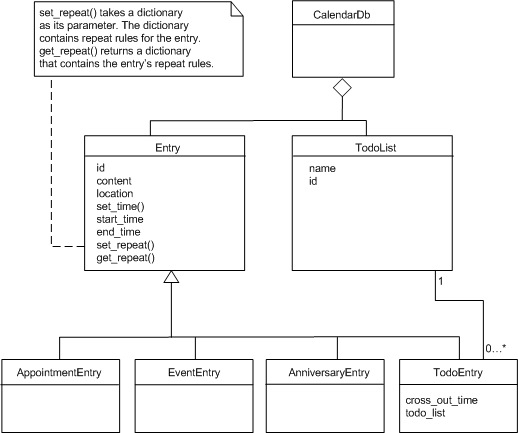
\includegraphics[width=10cm]{libcalendar-1}
\caption{The \module{calendar} module objects}
\label{libcalendar-1}
\end{figure}

Figure \ref{libcalendar-1} demonstrates the relationships of the 
\code{calendar} module objects. 

\subsection{Module Level Functions}
\label{subsec:calendarmodule}
The following free functions - functions that do not belong to any class 
- are defined in the \code{calendar} module:

\begin{funcdesc}{open}{\optional{filename=None, mode=None}}

Opens a calendar database and returns a new \class{CalendarDb} object.

If filename is \code{None}, the default database is opened.

If \var{filename} is given, it should be a full, absolute path name in
Unicode that specifies the calendar database to open. 

\var{mode} can be:

\begin{itemize}
\item \code{None}: Opens an existing calendar database.
\item \code{'c'}: Opens an existing calendar database, or creates it if it doesn't exist.
\item \code{'n'}: Creates a new, empty calendar database. If \var{filename} exists, the previous contents are erased.
\end{itemize}

\end{funcdesc}

\subsection{CalendarDb Objects}
\label{subsec:calendardb}

Calendar entries and todo lists are stored in a calendar database. There is 
one default calendar database but more calendar databases can be created by 
invoking \code{open} with parameters \code{'n' }or \code{'c'}. 

\begin{classdesc*}{CalendarDb}
\class{CalendarDb} objects have the following methods:

\begin{methoddesc}[CalendarDb]{add_appointment}{}

Creates and returns a new appointment entry \class{AppointmentEntry}. The 
entry is not added and saved into the database until \code{Entry.commit} is 
called.

\end{methoddesc}

\begin{methoddesc}[CalendarDb]{add_event}{}

Creates and returns a new event entry \class{EventEntry}. The entry is not added 
and saved into the database until \code{Entry.commit} is called.

\end{methoddesc}

\begin{methoddesc}[CalendarDb]{add_anniversary}{}

Creates and returns a new anniversary entry \class{AnniversaryEntry}. The entry 
is not added and saved into the database until \code{Entry.commit} is called.

\end{methoddesc}

\begin{methoddesc}[CalendarDb]{add_todo}{}

Creates and returns new todo entry \class{TodoEntry}. The entry is not added and 
saved into the database until \code{Entry.commit} is called.

\end{methoddesc}

\begin{methoddesc}[CalendarDb]{find_instances}{start_date, end_date, search_str=u''\optional{ ,appointments=0,events=0,anniversaries=0,todos=0}}

The parameters for this function include the start date, end date, search 
string, and optional parameters. The optional parameters define the entry 
types to be included into the search. By default all entry types are 
included. Returns a list that contains \class{Entry} instances found in the 
search. An instance is a dictionary that contains the entry ID and the 
datetime value. An entry may have several instances if it is repeated, for 
example once every week, etc. However, all the returned instances occur on 
the same day, i.e. on the first day between the start and end datetime 
values that contains instances. To search all instances between the initial 
start and end datetime values, you may have to execute several searches and 
change the start datetime value for each search. A match is detected if the 
search string is a substring of an entry's content. 

\end{methoddesc}

\begin{methoddesc}[CalendarDb]{monthly_instances}{month, appointments=0, events=0, anniversaries=0, todos=0}

The parameters for this function include \var{month} (float) and 
optional parameters. The optional parameters define the entry types to be 
returned. Returns a list that contains entry instances occurring during the 
specified calendar month.

\end{methoddesc}

\begin{methoddesc}[CalendarDb]{daily_instances}{day, appointments=0, events=0, anniversaries=0, todos=0}

The parameters for this function include \var{day} (float) and 
optional parameters. The optional parameters define the entry types to be 
returned. Returns a list that contains entry instances occurring on the 
specified day.

\end{methoddesc}

\begin{methoddesc}[CalendarDb]{add_todo_list}{\optional{name=None}}

Creates a new todo list. \var{name} sets the name of the todo list 
(Unicode). Returns the ID of the created todo list.

\end{methoddesc}

\begin{methoddesc}[CalendarDb]{export_vcalendars}{(int,...)}

Returns a \code{vcalendar} string that contains the specified entries in 
vCalendar format. The parameter for this function is a tuple that contains 
the entry IDs of the exported entries.

\end{methoddesc}

\begin{methoddesc}[CalendarDb]{import_vcalendars}{string}

Imports \code{vcalendar} entries, given in the string parameter, to the 
database. Returns a tuple that contains the unique IDs of the imported 
entries.

\end{methoddesc}

\begin{memberdesc}[CalendarDb]{todo_lists}

Contains a dictionary-like \code{TodoListDict} object for accessing
the todo lists of this database.

\end{memberdesc}

\begin{methoddesc}[CalendarDb]{__delitem__}{id}

Deletes the given calendar \code{Entry} from the database. \code{id} is the 
unique ID of the calendar \code{Entry}.

\end{methoddesc}

\begin{methoddesc}[CalendarDb]{__getitem__}{id}

Returns a calendar \code{Entry} object indicated by the unique ID. The returned 
object can be one of the following: \class{AppointmentEntry}, 
\class{EventEntry}, \class{AnniversaryEntry}, or \class{TodoEntry}. \code{id} is 
the unique ID of the calendar \code{Entry}. 

\end{methoddesc}

\begin{methoddesc}[CalendarDb]{compact}{}

Compacts the database file. The returned value (integer) indicates the 
success of compaction; a value other than zero means that the compaction was 
successful.

\end{methoddesc}

\end{classdesc*}

\subsection{Entry Objects}
\label{subsec:entry}

An \class{Entry} object represents a live view into the state of a single 
entry in the database. You can access the entries with an entry's unique ID. 
If you create a new entry using \code{db.add_appointment} etc., it is 
saved into the database only if you call the entry's \code{commit} method. 
In case an entry is already saved into the database, the autocommit mode is 
on by default and all the changes are automatically saved into the database, 
unless you call the entry's \code{begin} method. If you call the entry's 
\code{begin} method, the changes are not saved into the database until you 
call the entry's \code{commit} method. 

Database entries cannot be locked. In other words, other applications are 
able to make changes to the database entries you are using (not directly to 
the \class{EntryObjects} you are using, but to their representation in the 
database) at the same time you are modifying them, even if you use 
\code{begin} and \code{commit} methods. 

\begin{classdesc*}{Entry}
\class{Entry} objects have the following methods and properties:

\begin{memberdesc}[Entry]{content}

Sets or returns the entry's content text (Unicode).

\end{memberdesc}

\begin{methoddesc}[Entry]{commit}{}

Saves the entry or in case of a new entry adds the entry into the database. 
Note that this can be called only in case of a new entry, created with 
\code{db.add_appointment} etc., or after \code{begin} is called. 

\end{methoddesc}

\begin{methoddesc}[Entry]{rollback}{}

Undoes the changes made after last \code{commit}.

\end{methoddesc}

\begin{methoddesc}[Entry]{set_repeat}{dictionary}

Sets the repeat data of the entry. \var{dictionary} is a repeat data dictionary 
that contains all the repeat rules. For more information on repeat rules, see 
Section \ref{subsec:repeat}, Repeat Rules.

\end{methoddesc}

\begin{methoddesc}[Entry]{get_repeat}{}

Returns the repeat data dictionary of the entry.

\end{methoddesc}

\begin{memberdesc}[Entry]{location}

Sets or returns the entry's location data (Unicode), for example meeting 
room information. 

\end{memberdesc}

\begin{methoddesc}[Entry]{set_time}{start\optional{, end}}

Sets the start and end datetime values of the entry (floats). If only one 
parameter is given, the other will have the same value. 

In case of events, anniversaries, and todo entries the datetime values are 
truncated to corresponding date values.

\class{TodoEntries} can be made undated with 
\code{TodoEntry.set_time(None)}. Making the todo entry undated means 
removing the start and end date and all the repeat rules.

\end{methoddesc}

\begin{memberdesc}[Entry]{start_time}

The start datetime value (float) of the entry or \code{None} if 
the start datetime of the entry is not set.

\end{memberdesc}

\begin{memberdesc}[Entry]{end_time}

The end datetime value (float) of the entry or \code{None} if the 
end datetime of the entry is not set.

\end{memberdesc}

\begin{memberdesc}[Entry]{id}

The unique ID of the entry.

\end{memberdesc}

\begin{memberdesc}[Entry]{last_modified}

The datetime value (float) of the entry's last modification in 
universal time.

\end{memberdesc}

\begin{memberdesc}[Entry]{alarm}

The alarm datetime value (float) for the entry. \code{None} if \code{alarm} is 
not set. Alternatively removes the alarm if the value is set to \code{None}. 

Alarms can be set to all \class{Entry} types. However, only alarms set to 
Appointments and Anniversaries will actually cause an alarm; this is similar 
to the Calendar application in your Nokia device, which allows you to set an 
alarm only for Meetings and Anniversaries. In addition, alarms set to any 
entries residing in a database other than the default database do not cause 
actual alarms either.

\end{memberdesc}

\begin{memberdesc}[Entry]{priority}

The priority of the entry, which can be an integer ranging from 0 to 255. Native 
Phonebook and Calendar applications in Nokia devices use value 1 for high 
priority, 2 for normal priority, and 3 for low priority. 

\end{memberdesc}

\begin{memberdesc}[Entry]{crossed_out}

The crossed out value of an entry. A value that is interpreted as false means 
that the entry is not crossed out, whereas a value that is interpreted as true 
means that the entry is crossed out. Note that \class{TodoEntries} must also 
have a cross-out time while the other entry types cannot have one. If 
\class{TodoEntry} is crossed out using this method, the moment of crossing out 
is set to the cross-out time of the \class{TodoEntry}. See also Section 
\ref{subsubsec:todoentry}, TodoEntry, \code{cross_out_time}.

\end{memberdesc}

\begin{memberdesc}[Entry]{replication}

Sets or returns the entry's replication status, which can be one of the 
following: \code{'open'}, \code{'private',} or \code{'restricted'}.

\end{memberdesc}

\begin{methoddesc}[Entry]{as_vcalendar}{}

Returns this entry as a vCalendar string.

\end{methoddesc}

\end{classdesc*}

\subsubsection{AppointmentEntry Objects}
\label{subsubsec:appointmententry}

\begin{classdesc*}{AppointmentEntry}
\end{classdesc*}

\class{AppointmentEntry} class contains no additional methods compared to 
the \class{Entry} class from which it is derived.

\subsubsection{EventEntry}
\label{subsubsec:evententry}

\begin{classdesc*}{EventEntry}
\end{classdesc*}

\class{EventEntry} class contains no additional methods compared to the 
\class{Entry} class from which it is derived.

\subsubsection{AnniversaryEntry}
\label{subsubsec:anniversaryentry}

\begin{classdesc*}{AnniversaryEntry}
\end{classdesc*}

\class{AnniversaryEntry} class contains no additional methods compared to 
the \class{Entry} class from which it is derived.

\subsubsection{TodoEntry}
\label{subsubsec:todoentry}

\class{TodoEntry}objects represent todo entry types. They have additional 
properties compared to the \class{Entry} class from which they are derived.

\begin{classdesc*}{TodoEntry}
\class{TodoEntry}objects have the following additional properties:

\begin{memberdesc}[TodoEntry]{cross_out_time}

The cross-out date value of the entry. The value can be \code{None} meaning that 
the entry is not crossed out, or the cross-out date (float). The set value must 
be date (float). Setting a cross-out time also crosses out the entry. See also 
Section \ref{subsec:entry}, Entry Object, \code{crossed_out}.

\end{memberdesc}

\begin{memberdesc}[TodoEntry]{todo_list}

The ID of the todo list to which this entry belongs.

\end{memberdesc}

\end{classdesc*}

\subsubsection{TodoListDict}
\label{subsubsec:todolistdict}

\class{TodoListDict} objects are dictionary-like objects that enable 
accessing todo lists. 

\begin{classdesc*}{TodoListDict}
\class{TodoListDict} objects have the following property:

\begin{memberdesc}[TodoListDict]{default_list}

The ID of the default todo list.

\end{memberdesc}

\end{classdesc*}

\subsubsection{TodoList}
\label{subsubsec:todolist}

\class{TodoList} objects are dictionary-like objects that enable 
accessesing todo lists. 

\begin{classdesc*}{TodoList}
\code{TodoList} objects have the following properties:

\begin{memberdesc}[TodoList]{name}

The name of the todo list as a Unicode string.

\end{memberdesc}

\begin{memberdesc}[TodoList]{id}

Returns the ID of the todo list as an integer.

\end{memberdesc}

\end{classdesc*}

\subsection{Repeat Rules}
\label{subsec:repeat}

Repeat rules specify an entry's repeat status, that is, the recurrence of 
the entry. There are six repeat types: 

\begin{itemize}
\item \code{daily}: repeated daily
\item \code{weekly}: repeat on the specified days of the week, such as Monday and Wednesday, etc.
\item \code{monthly_by_dates}: repeat monthly on the specified dates, such as the 15th and 17th day of the month
\item \code{monthly_by_days}: repeat monthly on the specified days, such as the fourth Wednesday of the month, or the last Monday of the month
\item \code{yearly_by_date}: repeat yearly on the specified date, such as December 24
\item \code{yearly_by_day}: repeat yearly on the specified day, such as every third Tuesday of May
\end{itemize}

There are exceptions to repeat rules. For example, you can specify the 
datetime value (float) in such a way that the entry is not repeated on a 
specific day even if the repeat rule would specify otherwise.

You must set the start and end dates (floats) of the repeat. The end date 
can also be set to \code{None} to indicate that the repeating continues 
forever. You can set \code{interval} defining how often the repeat occurs, 
for example in a daily repeat: \code{1} means every day, \code{2} means 
every second day, etc. You can also set the \code{days} specifier which 
lets you explicitly specify the repeat days; for example in a weekly repeat 
you can set \code{"days":[0,2]} which sets the repeat to occur on Mondays 
and Wednesdays. If you do not set the \code{days} specifier, the repeat 
days are calculated automatically based on the start date.

You can modify repeat data by calling \code{rep_data = 
entry.get_repeat()}, then making changes to \code{rep_data} 
dictionary, and then calling \code{entry.set_repeat(rep_data)}.

Repeating can be cancelled by calling \code{entry.set_repeat} with a 
parameter that is interpreted to be false, such as 
\code{entry.set_repeat(None)}.

Repeat definition examples:

\begin{verbatim}

repeat = {"type":"daily", #repeat type
          "exceptions":[exception_day, exception_day+2*24*60*60],  
          #no appointment on those days
          "start":appt_start_date, #start of the repeat
          "end":appt_start_date+30*24*60*60, #end of the repeat
          "interval":1} #interval (1=every day, 2=every second day etc.)

repeat = {"type":"weekly", #repeat type
          "days":[0,1], #which days in a week (Monday, Tuesday)
          "exceptions":[exception_day], #no appointment on that day
          "start":appt_start_date, #start of the repeat
          "end":appt_start_date+30*24*60*60, #end of the repeat
          "interval":1}  
          #interval (1=every week, 2=every second week etc.) 

repeat = {"type":"monthly_by_days", #repeat type
          # appointments on second Tuesday and last Monday of the month
          "days":[{"week":1, "day":1},{"week":4, "day":0}],
          "exceptions":[exception_day], #no appointment on that day 
          "start":appt_start_date, #start of the repeat
          "end":appt_start_date+30*24*60*60, #end of the repeat
          "interval":1}  
          #interval (1=every month, 2=every second month etc.)

repeat = {"type":"monthly_by_dates", #repeat type
          "days":[0,15],  
          # appointments on the 1st and 16th day of the month.
          "exceptions":[exception_day], #no appointment on that day
          "start":appt_start_date, #start of the repeat
          "end":appt_start_date+30*24*60*60, #end of the repeat
          "interval":1}  
          #interval (1=every month, 2=every second month etc.)

repeat = {"type":"yearly_by_date", #repeat type
          "exceptions":[exception_day], #no appointment on that day 
          "start":appt_start_date, #start of the repeat
          "end":appt_start_date+3*365*24*60*60, #end of the repeat
          "interval":1}  
          #interval (1=every year, 2=every second year etc.)

repeat = {"type":"yearly_by_day", #repeat type
          # appointments on the second Tuesday of February
          "days":{"day":1, "week":1, "month":1},
          "exceptions":[exception_day], #no appointment on that day 
          "start":appt_start_date, #start of the repeat
          "end":appt_start_date+3*365*24*60*60, #end of the repeat
          "interval":1}  
          #interval (1=every year, 2=every second year etc.)

\end{verbatim}

% Copyright (c) 2006 Nokia Corporation
%
% Licensed under the Apache License, Version 2.0 (the "License");
% you may not use this file except in compliance with the License.
% You may obtain a copy of the License at
%
%     http://www.apache.org/licenses/LICENSE-2.0
%
% Unless required by applicable law or agreed to in writing, software
% distributed under the License is distributed on an "AS IS" BASIS,
% WITHOUT WARRANTIES OR CONDITIONS OF ANY KIND, either express or implied.
% See the License for the specific language governing permissions and
% limitations under the License.

\section{\module{calendar for EKA2} ---
  Access to calendar related services}
\label{sec:calendareka2}

\declaremodule{extension}{calendar}
\platform{S60}
\modulesynopsis{A calendar related services package.}

The \module{calendar} module offers an API to calendar services. The 
\module{calendar} module represents a Symbian agenda database as a 
dictionary-like \class{CalendarDb} object, which contains \class{Entry}
objects and which is indexed using the unique IDs of those objects. There 
are five types of entry objects: \class{AppointmentEntry}, 
\class{EventEntry}, \class{AnniversaryEntry}, \class{ReminderEntry},
 and \class{TodoEntry}. 

\class{CalendarDb} objects represent a live view into the database. If an 
entry is changed outside your Python application, the changes are visible 
immediately, and conversely any changes you commit into the database are 
visible immediately to other applications. 

All time parameters use Unix time unless stated otherwise. For more 
information on Unix time, see Section \ref{subsec:datetime}, 
Date and Time.

\subsection{Module Level Functions}
\label{subsec:calendarmodule}
The following free functions - functions that do not belong to any class 
- are defined in the \code{calendar} module:

\begin{funcdesc}{open}{\optional{filename=None, mode=None}}

Opens a calendar database and returns a new \class{CalendarDb} object.

If filename is \code{None}, the default database is opened.

If \var{filename} is given, it should contain drive letter, colon and file's name, 
but no absolute path.

\var{mode} can be:

\begin{itemize}
\item \code{None}: Opens an existing calendar database.
\item \code{'c'}: Opens an existing calendar database, or creates it if it doesn't exist.
\item \code{'n'}: Creates a new, empty calendar database. If \var{filename} exists, the previous contents are erased.
\end{itemize}

\end{funcdesc}

\subsection{CalendarDb Objects}
\label{subsec:calendardb}

Calendar entries are stored in a calendar database. There is 
one default calendar database but more calendar databases can be created by 
invoking \code{open} with parameters \code{'n' }or \code{'c'}. 

\begin{classdesc*}{CalendarDb}
\class{CalendarDb} objects have the following methods:

\begin{methoddesc}[CalendarDb]{add_appointment}{}

Creates and returns a new appointment entry \class{AppointmentEntry}. The 
entry is not added and saved into the database until \code{Entry.commit} is 
called.

\end{methoddesc}

\begin{methoddesc}[CalendarDb]{add_event}{}

Creates and returns a new event entry \class{EventEntry}. The entry is not added 
and saved into the database until \code{Entry.commit} is called.

\end{methoddesc}

\begin{methoddesc}[CalendarDb]{add_anniversary}{}

Creates and returns a new anniversary entry \class{AnniversaryEntry}. The entry 
is not added and saved into the database until \code{Entry.commit} is called.

\end{methoddesc}

\begin{methoddesc}[CalendarDb]{add_todo}{}

Creates and returns new todo entry \class{TodoEntry}. The entry is not added and 
saved into the database until \code{Entry.commit} is called.

\end{methoddesc}

\begin{methoddesc}[CalendarDb]{add_reminder}{}

Creates and returns new reminder entry \class{ReminderEntry}. The entry is not added and 
saved into the database until \code{Entry.commit} is called.

\end{methoddesc}

\begin{methoddesc}[CalendarDb]{find_instances}{start_date, end_date, search_str=u''\optional{ ,appointments=0,events=0,anniversaries=0,todos=0,reminders=0}}

The parameters for this function include the start date, end date, search 
string, and optional parameters. The optional parameters define the entry 
types to be included into the search. By default all entry types are 
included. Returns a list that contains \class{Entry} instances found in the 
search. An instance is a dictionary that contains the entry ID and the 
datetime value. An entry may have several instances if it is repeated, for 
example once every week, etc. 

\end{methoddesc}

\begin{methoddesc}[CalendarDb]{monthly_instances}{month, appointments=0, events=0, anniversaries=0, todos=0, reminders=0}

The parameters for this function include \var{month} (float) and 
optional parameters. The optional parameters define the entry types to be 
returned. Returns a list that contains entry instances occurring during the 
specified calendar month.

\end{methoddesc}

\begin{methoddesc}[CalendarDb]{daily_instances}{day, appointments=0, events=0, anniversaries=0, todos=0}

The parameters for this function include \var{day} (float) and 
optional parameters. The optional parameters define the entry types to be 
returned. Returns a list that contains entry instances occurring on the 
specified day.

\end{methoddesc}

\begin{methoddesc}[CalendarDb]{export_vcalendars}{(int,...)}

Returns a \code{vcalendar} string that contains the specified entries in 
vCalendar format. The parameter for this function is a tuple that contains 
the entry IDs of the exported entries.

\end{methoddesc}

\begin{methoddesc}[CalendarDb]{import_vcalendars}{string}

Imports \code{vcalendar} entries, given in the string parameter, to the 
database. Returns a list that contains the unique IDs of the imported 
entries.

\end{methoddesc}

\begin{methoddesc}[CalendarDb]{__delitem__}{id}

Deletes the given calendar \code{Entry} from the database. \code{id} is the 
unique ID of the calendar \code{Entry}.

\end{methoddesc}

\begin{methoddesc}[CalendarDb]{__getitem__}{id}

Returns a calendar \code{Entry} object indicated by the unique ID. The returned 
object can be one of the following: \class{AppointmentEntry}, 
\class{EventEntry}, \class{AnniversaryEntry}, \class{ReminderEntry}, 
or \class{TodoEntry}. \code{id} is the unique ID of the calendar \code{Entry}. 

\end{methoddesc}

\end{classdesc*}

\subsection{Entry Objects}
\label{subsec:entry}

An \class{Entry} object represents a live view into the state of a single 
entry in the database. You can access the entries with an entry's unique ID. 
If you create a new entry using \code{db.add_appointment} etc., it is 
saved into the database only if you call the entry's \code{commit} method. 
In case an entry is already saved into the database, the autocommit mode is 
on by default and all the changes are automatically saved into the database, 
unless you call the entry's \code{begin} method. If you call the entry's 
\code{begin} method, the changes are not saved into the database until you 
call the entry's \code{commit} method. 

Database entries cannot be locked. In other words, other applications are 
able to make changes to the database entries you are using (not directly to 
the \class{EntryObjects} you are using, but to their representation in the 
database) at the same time you are modifying them, even if you use 
\code{begin} and \code{commit} methods. 

\begin{classdesc*}{Entry}
\class{Entry} objects have the following methods and properties:

\begin{memberdesc}[Entry]{content}

Sets or returns the entry's content text (Unicode).

\end{memberdesc}

\begin{methoddesc}[Entry]{commit}{}

Saves the entry or in case of a new entry adds the entry into the database. 
Note that this can be called only in case of a new entry, created with 
\code{db.add_appointment} etc., or after \code{begin} is called. 

\end{methoddesc}

\begin{methoddesc}[Entry]{rollback}{}

Undoes the changes made after last \code{commit}.

\end{methoddesc}

\begin{methoddesc}[Entry]{set_repeat}{dictionary}

Sets the repeat data of the entry. \var{dictionary} is a repeat data dictionary 
that contains all the repeat rules. For more information on repeat rules, see 
Section \ref{subsec:repeat}, Repeat Rules.

\end{methoddesc}

\begin{methoddesc}[Entry]{get_repeat}{}

Returns the repeat data dictionary of the entry.

\end{methoddesc}

\begin{memberdesc}[Entry]{location}

Sets or returns the entry's location data (Unicode), for example meeting 
room information. 

\end{memberdesc}

\begin{methoddesc}[Entry]{set_time}{start\optional{, end}}

Sets the start and end datetime values of the entry (floats). If only one 
parameter is given, the other will have the same value. 

In case of events, anniversaries, and todo entries the datetime values are 
truncated to corresponding date values.

\class{TodoEntries} can be made undated with 
\code{TodoEntry.set_time(None)}. Making the todo entry undated means 
removing the start and end date and all the repeat rules.

\end{methoddesc}

\begin{memberdesc}[Entry]{start_time}

The start datetime value (float) of the entry or \code{None} if 
the start datetime of the entry is not set.

\end{memberdesc}

\begin{memberdesc}[Entry]{end_time}

The end datetime value (float) of the entry or \code{None} if the 
end datetime of the entry is not set.

\end{memberdesc}

\begin{memberdesc}[Entry]{id}

The unique ID of the entry.

\end{memberdesc}

\begin{memberdesc}[Entry]{last_modified}

The datetime value (float) of the entry's last modification in 
universal time.

\end{memberdesc}

\begin{memberdesc}[Entry]{originating}

An integer value indicating if the entry is an originating entry
or a modifying entry.

\end{memberdesc}

\begin{memberdesc}[Entry]{alarm}

The alarm datetime value (float) for the entry. \code{None} if \code{alarm} is 
not set. Alternatively removes the alarm if the value is set to \code{None}. 

Alarms can be set to all \class{Entry} types. However, only alarms set to 
Appointments and Anniversaries will actually cause an alarm; this is similar 
to the Calendar application in your Nokia device, which allows you to set an 
alarm only for Meetings and Anniversaries. In addition, alarms set to any 
entries residing in a database other than the default database do not cause 
actual alarms either.

\end{memberdesc}

\begin{memberdesc}[Entry]{priority}

The priority of the entry, which can be an integer ranging from 0 to 255. Native 
Phonebook and Calendar applications in Nokia devices use value 1 for high 
priority, 2 for normal priority, and 3 for low priority. 

\end{memberdesc}

\begin{memberdesc}[Entry]{crossed_out}

The crossed out value of an entry. Only valid for todo entries.
A value that is interpreted as false means 
that the entry is not crossed out, whereas a value that is interpreted as true 
means that the entry is crossed out. Note that \class{TodoEntries} must also 
have a cross-out time. If \class{TodoEntry} is crossed out using this method, 
the moment of crossing out is set to the cross-out time of the \class{TodoEntry}. 
See also Section \ref{subsubsec:todoentry}, TodoEntry, \code{cross_out_time}.

\end{memberdesc}

\begin{memberdesc}[Entry]{replication}

Sets or returns the entry's replication status, which can be one of the 
following: \code{'open'}, \code{'private',} or \code{'restricted'}.

\end{memberdesc}

\begin{methoddesc}[Entry]{as_vcalendar}{}

Returns this entry as a vCalendar string.

\end{methoddesc}

\end{classdesc*}

\subsubsection{AppointmentEntry Objects}
\label{subsubsec:appointmententry}

\begin{classdesc*}{AppointmentEntry}
\end{classdesc*}

\class{AppointmentEntry} class contains no additional methods compared to 
the \class{Entry} class from which it is derived.

\subsubsection{EventEntry}
\label{subsubsec:evententry}

\begin{classdesc*}{EventEntry}
\end{classdesc*}

\class{EventEntry} class contains no additional methods compared to the 
\class{Entry} class from which it is derived.

\subsubsection{AnniversaryEntry}
\label{subsubsec:anniversaryentry}

\begin{classdesc*}{AnniversaryEntry}
\end{classdesc*}

\class{AnniversaryEntry} class contains no additional methods compared to 
the \class{Entry} class from which it is derived.

\subsubsection{ReminderEntry}
\label{subsubsec:reminderentry}

\begin{classdesc*}{ReminderEntry}
\end{classdesc*}

\class{ReminderEntry} class contains no additional methods compared to 
the \class{Entry} class from which it is derived.

\subsubsection{TodoEntry}
\label{subsubsec:todoentry}

\class{TodoEntry}objects represent todo entry types. They have additional 
properties compared to the \class{Entry} class from which they are derived.

\begin{classdesc*}{TodoEntry}
\class{TodoEntry}objects have the following additional properties:

\begin{memberdesc}[TodoEntry]{cross_out_time}

The cross-out date value of the entry. The value can be \code{None} meaning that 
the entry is not crossed out, or the cross-out date (float). The set value must 
be date (float). Setting a cross-out time also crosses out the entry. See also 
Section \ref{subsec:entry}, Entry Object, \code{crossed_out}.

\end{memberdesc}

\end{classdesc*}


\subsection{Repeat Rules}
\label{subsec:repeat}

Repeat rules specify an entry's repeat status, that is, the recurrence of 
the entry. There are six repeat types: 

\begin{itemize}
\item \code{daily}: repeated daily
\item \code{weekly}: repeat on the specified days of the week, such as Monday and Wednesday, etc.
\item \code{monthly_by_dates}: repeat monthly on the specified dates, such as the 15th and 17th day of the month
\item \code{monthly_by_days}: repeat monthly on the specified days, such as the fourth Wednesday of the month, or the last Monday of the month
\item \code{yearly_by_date}: repeat yearly on the specified date, such as December 24
\item \code{yearly_by_day}: repeat yearly on the specified day, such as every third Tuesday of May
\end{itemize}

There are exceptions to repeat rules. For example, you can specify the 
datetime value (float) in such a way that the entry is not repeated on a 
specific day even if the repeat rule would specify otherwise.

You must set the start and end dates (floats) of the repeat. The end date 
can also be set to \code{None} to indicate that the repeating continues 
forever. You can set \code{interval} defining how often the repeat occurs, 
for example in a daily repeat: \code{1} means every day, \code{2} means 
every second day, etc. You can also set the \code{days} specifier which 
lets you explicitly specify the repeat days; for example in a weekly repeat 
you can set \code{"days":[0,2]} which sets the repeat to occur on Mondays 
and Wednesdays. If you do not set the \code{days} specifier, the repeat 
days are calculated automatically based on the start date.

You can modify repeat data by calling \code{rep_data = 
entry.get_repeat()}, then making changes to \code{rep_data} 
dictionary, and then calling \code{entry.set_repeat(rep_data)}.

Repeating can be cancelled by calling \code{entry.set_repeat} with a 
parameter that is interpreted to be false, such as 
\code{entry.set_repeat(None)}.

Repeat definition examples:

\begin{verbatim}

repeat = {"type":"daily", #repeat type
          "exceptions":[exception_day, exception_day+2*24*60*60],  
          #no appointment on those days
          "start":appt_start_date, #start of the repeat
          "end":appt_start_date+30*24*60*60, #end of the repeat
          "interval":1} #interval (1=every day, 2=every second day etc.)

repeat = {"type":"weekly", #repeat type
          "days":[0,1], #which days in a week (Monday, Tuesday)
          "exceptions":[exception_day], #no appointment on that day
          "start":appt_start_date, #start of the repeat
          "end":appt_start_date+30*24*60*60, #end of the repeat
          "interval":1}  
          #interval (1=every week, 2=every second week etc.) 

repeat = {"type":"monthly_by_days", #repeat type
          # appointments on second Tuesday and last Monday of the month
          "days":[{"week":1, "day":1},{"week":4, "day":0}],
          "exceptions":[exception_day], #no appointment on that day 
          "start":appt_start_date, #start of the repeat
          "end":appt_start_date+30*24*60*60, #end of the repeat
          "interval":1}  
          #interval (1=every month, 2=every second month etc.)

repeat = {"type":"monthly_by_dates", #repeat type
          "days":[0,15],  
          # appointments on the 1st and 16th day of the month.
          "exceptions":[exception_day], #no appointment on that day
          "start":appt_start_date, #start of the repeat
          "end":appt_start_date+30*24*60*60, #end of the repeat
          "interval":1}  
          #interval (1=every month, 2=every second month etc.)

repeat = {"type":"yearly_by_date", #repeat type
          "exceptions":[exception_day], #no appointment on that day 
          "start":appt_start_date, #start of the repeat
          "end":appt_start_date+3*365*24*60*60, #end of the repeat
          "interval":1}  
          #interval (1=every year, 2=every second year etc.)

repeat = {"type":"yearly_by_day", #repeat type
          # appointments on the second Tuesday of February
          "days":{"day":1, "week":1, "month":1},
          "exceptions":[exception_day], #no appointment on that day 
          "start":appt_start_date, #start of the repeat
          "end":appt_start_date+3*365*24*60*60, #end of the repeat
          "interval":1}  
          #interval (1=every year, 2=every second year etc.)

\end{verbatim}

% Copyright (c) 2005 Nokia Corporation
%
% Licensed under the Apache License, Version 2.0 (the "License");
% you may not use this file except in compliance with the License.
% You may obtain a copy of the License at
%
%     http://www.apache.org/licenses/LICENSE-2.0
%
% Unless required by applicable law or agreed to in writing, software
% distributed under the License is distributed on an "AS IS" BASIS,
% WITHOUT WARRANTIES OR CONDITIONS OF ANY KIND, either express or implied.
% See the License for the specific language governing permissions and
% limitations under the License.

\section{\module{e32db} ---
  Interface to the Symbian native DB}
\label{sec:e32db}

\declaremodule{extension}{e32db}
\platform{S60}
\modulesynopsis{Interface to the Symbian native DB}

\label{sec:mylabel3}
The \module{e32db} module provides an API for relational database 
manipulation with a restricted SQL syntax. For details of DBMS support, see 
the S60 SDK documentation. For examples on using this module, see \cite{PyS60Prog}.

The \module{e32db} module defines the following functions:

\begin{funcdesc}{format_rawtime}{timevalue}
Formats \var{timevalue} (Symbian time) according to the current 
system's date/time formatting rules and returns it as a Unicode string.
\end{funcdesc}

\begin{funcdesc}{format_time}{timevalue}
Formats \var{timevalue} according to the current system's date/time 
formatting rules and returns it as a Unicode string.
\end{funcdesc}

\subsection{Dbms Objects}
\label{subsec:mylabel13}

\begin{classdesc}{Dbms}{}
Creates a Dbms object. Dbms objects support basic 
operations on a database. 
\end{classdesc}

Dbms objects have the following methods:

\begin{methoddesc}[Dbms]{begin}{}
Begins a transaction on the database.
\end{methoddesc}

\begin{methoddesc}[Dbms]{close}{}
Closes the database object. It is safe to try to close a database object 
even if it is not open.
\end{methoddesc}

\begin{methoddesc}[Dbms]{commit}{}
Commits the current transaction.
\end{methoddesc}

\begin{methoddesc}[Dbms]{compact}{}
Compacts the database, reclaiming unused space in the database file. 
\end{methoddesc}

\begin{methoddesc}[Dbms]{create}{dbname}
Creates a database with path \var{dbname}.
\end{methoddesc}

\begin{methoddesc}[Dbms]{execute}{query}
Executes an SQL \var{query}. On success, returns \code{0} if a DDL
(SQL schema update) statement was executed. Returns the number of rows
inserted, updated, or deleted, if a DML (SQL data update) statement
was executed.
\end{methoddesc}

\begin{methoddesc}[Dbms]{open}{dbname}
Opens the database in file \var{dbname}. This should be a full 
Unicode path name, for example, \code{u'c:\e\e foo.db'}.
\end{methoddesc}

\begin{methoddesc}[Dbms]{rollback}{}
Rolls back the current transaction.
\end{methoddesc}

\subsection{DB_view Objects}
\label{subsec:mylabel14}

\begin{classdesc}{Db_view}{}
Creates a \class{Db_view} object. \class{DB_view} objects generate 
rowsets from a SQL query. They provide functions to parse and evaluate the 
rowsets.
\end{classdesc}

Db_view objects have the following methods:

\begin{methoddesc}[Db_view]{col}{column}
Returns the value in \var{column}. The first column of the rowset has the index 
\code{1}. If the type of the column is not supported, a \exception{TypeError} is 
raised. See Table \ref{tab:sqltypes} for a list of supported data types.
\end{methoddesc}

\begin{methoddesc}[Db_view]{col_count}{}
Returns the number of columns defined in the rowset.
\end{methoddesc}

\begin{methoddesc}[Db_view]{col_length}{column}
Gets the length of the value in \var{column}. Empty columns have 
a length of zero; non-empty numerical and date/time columns have a length of 
1. For text columns, the length is the character count, and for binary 
columns, the length is the byte count.
\end{methoddesc}

\begin{methoddesc}[Db_view]{col_raw}{column}
Extracts the value of \var{column} as raw binary data, and 
returns it as a Python string. The first column of the rowset has the index 
1. See Table \ref{tab:sqltypes} for a list of supported data types.
\end{methoddesc}

\begin{methoddesc}[Db_view]{col_rawtime}{column}
Extracts the value of a date/time column at index \var{column} as a
long integer, which represents the raw Symbian time value. The first
column of the rowset has the index 1.  See Table \ref{tab:sqltypes} for a list of the
supported data types.
\end{methoddesc}

\begin{methoddesc}[Db_view]{col_type}{column}
Returns the numeric type of the given column as an integer from a 
Symbian-specific list of types. This function is used in the implementation 
of method \method{col}.
\end{methoddesc}

\begin{methoddesc}[Db_view]{count_line}{}
Returns the number of rows available in the rowset.
\end{methoddesc}

\begin{methoddesc}[Db_view]{first_line}{}
Positions the cursor on the first row in the rowset.
\end{methoddesc}

\begin{methoddesc}[Db_view]{get_line}{}
Gets the current row data for access.
\end{methoddesc}

\begin{methoddesc}[Db_view]{is_col_null}{column}
Tests whether \var{column} is empty. Empty columns can be 
accessed like normal columns. Empty numerical columns return a \code{0} or 
an equivalent value, and text and binary columns have a zero length.
\end{methoddesc}

\begin{methoddesc}[Db_view]{next_line}{}
Moves the cursor to the next row in the rowset.
\end{methoddesc}

\begin{methoddesc}[Db_view]{prepare}{db, query}
Prepares the view object for evaluating an SQL select statement. 
\var{db} is a \class{Dbms} object and \var{query}
the SQL query to be executed.
\end{methoddesc}

\subsection{Mapping Between SQL and Python Data Types }
\label{subsec:mapping}
See Table \ref{tab:sqltypes} for a summary of mapping between SQL and 
Python data types. The \method{col} function can extract any value except 
\code{LONG VARBINARY} and return it as the proper Python value. In 
addition, the \method{col_raw} function can extract any column type 
except \code{LONG VARCHAR} and \code{LONG VARBINARY} as raw binary data 
and return it as a Python string.

Inserting, updating, or searching for \code{BINARY}, \code{VARBINARY}, 
or \code{LONG VARBINARY} values is not supported. \code{BINARY} and 
\code{VARBINARY} values can be read with \method{col} or 
\method{col_raw}.

\begin{table}[htbp]
\begin{center}
\begin{tabular}{|p{117pt}|p{144pt}|p{99pt}|p{63pt}|}
\hline
SQL type& 
Symbian column type (in the DBMS C++ API)& 
Python type& 
Supported \\
\hline
\textsf{BIT}& 
\textsf{EDbColBit}& 
\raisebox{-10.50ex}[0cm][0cm]{int}& 
\raisebox{-27.00ex}[0cm][0cm]{yes} \\
\cline{1-2} 
\textsf{TINYINT}& 
\textsf{EDbColInt8}& 
 & 
  \\
\cline{1-2} 
\textsf{UNSIGNED TINYINT}& 
\textsf{EDbColUint8}& 
 & 
  \\
\cline{1-2} 
\textsf{SMALLINT}& 
\textsf{EDbColInt16}& 
 & 
  \\
\cline{1-2} 
\textsf{UNSIGNED SMALLINT}& 
\textsf{EDbColUint16}& 
 & 
  \\
\cline{1-2} 
\textsf{INTEGER}& 
\textsf{EDbColInt32}& 
 & 
  \\
\cline{1-2} 
\textsf{UNSIGNED INTEGER}& 
\textsf{EDbColUint32}& 
 & 
  \\
\cline{1-2} 
\textsf{COUNTER}& 
\textsf{EDbColUint32 (}with the\textsf{ TDbCol::EAutoIncrement }attribute\textsf{)}& 
 & 
  \\
\cline{1-3} 
\textsf{BIGINT}& 
\textsf{EDbColInt64}& 
long& 
  \\
\cline{1-3} 
\textsf{REAL}& 
\textsf{EDbColReal32}& 
\raisebox{-4.50ex}[0cm][0cm]{float  \par }& 
  \\
\cline{1-2} 
\textsf{FLOAT}& 
\raisebox{-3.00ex}[0cm][0cm]{\textsf{EDbColReal64} \par \textsf{}}& 
 & 
  \\
\cline{1-1} 
\textsf{DOUBLE}& 
 & 
 & 
  \\
\cline{1-1} 
\textsf{DOUBLE PRECISION}& 
 & 
 & 
  \\
\cline{1-3} 
\textsf{DATE}& 
\raisebox{-3.00ex}[0cm][0cm]{\textsf{EDbColDateTime} \par \textsf{}}& 
\raisebox{-3.00ex}[0cm][0cm]{float \par (or long, with \textsf{col_rawtime()})}& 
  \\
\cline{1-1} 
\textsf{TIME}& 
 & 
 & 
  \\
\cline{1-1} 
\textsf{TIMESTAMP}& 
 & 
 & 
  \\
\cline{1-3} 
\textsf{CHAR(n)}& 
\raisebox{-1.50ex}[0cm][0cm]{\textsf{EDbColText}}& 
\raisebox{-3.00ex}[0cm][0cm]{Unicode}& 
  \\
\cline{1-1} 
\textsf{VARCHAR(n)}& 
 & 
 & 
  \\
\cline{1-2} 
\textsf{LONG VARCHAR}& 
\textsf{EDbColLongText}& 
 & 
  \\
\hline
\textsf{BINARY(n)}& 
\raisebox{-1.50ex}[0cm][0cm]{\textsf{EDbColBinary} \par \textsf{}}& 
\raisebox{-1.50ex}[0cm][0cm]{str}& 
\raisebox{-1.50ex}[0cm][0cm]{read only} \\
\cline{1-1} 
\textsf{VARBINARY(n)}& 
 & 
 & 
  \\
\hline
\textsf{LONG VARBINARY}& 
\textsf{EDbColLongBinary}& 
n/a& 
no \\
\hline
\end{tabular}
\caption{Mapping between SQL and Python types}
\label{tab:sqltypes}
\end{center}
\end{table}


\subsection{Date and Time Handling}
\label{subsec:mylabel15}
The functions \method{col} and \textsf{format_time} use Unix time, 
seconds since January 1, 1970, 00:00:00 UTC, as the time format. Internally 
the database uses the native Symbian time representation that provides 
greater precision and range than the Unix time. The native Symbian time 
format is a 64-bit value that represents microseconds since January 1st 0 AD 
00:00:00 local time, nominal Gregorian. BC dates are represented by negative 
values. Since converting this format to Unix time and back may cause slight 
round-off errors, you have to use the functions \function{col_rawtime} and 
\function{format_rawtime} if you need to be able to handle these values 
with full precision.

The representation of date and time literals in SQL statements depends on 
the current system date and time format. Note that the only accepted 
ordering of day, month, and year is the one that the system is currently 
configured to use. Dates in other order are rejected. The recommended way to 
form date/time literals for SQL statements is to use the functions 
\function{format_time} or \function{format_rawtime} that format the given 
date/time values properly according to the current system's date/time format 
settings.

% Copyright (c) 2005 Nokia Corporation
%
% Licensed under the Apache License, Version 2.0 (the "License");
% you may not use this file except in compliance with the License.
% You may obtain a copy of the License at
%
%     http://www.apache.org/licenses/LICENSE-2.0
%
% Unless required by applicable law or agreed to in writing, software
% distributed under the License is distributed on an "AS IS" BASIS,
% WITHOUT WARRANTIES OR CONDITIONS OF ANY KIND, either express or implied.
% See the License for the specific language governing permissions and
% limitations under the License.

\section{\module{e32dbm} ---
  DBM implemented using the Symbian native DBMS}
\label{sec:e32dbm}

\declaremodule{}{e32dbm}
\platform{S60}
\modulesynopsis{DBM implemented using the Symbian native DBMS}

The \module{e32dbm} module provides a DBM API that uses the native
Symbian RDBMS as its storage back-end. The module API resembles that
of the \refmodule{gdbm} module. The main differences are:

\begin{itemize}
\item The \method{firstkey()} - \method{nextkey()} interface for iterating through keys is not supported. Use the \code{"for key in db"} idiom or the \method{keys} or \method{keysiter} methods instead.
\item This module supports a more complete set of dictionary features than \refmodule{gdbm}
\item The values are always stored as Unicode, and thus the values returned are Unicode strings even if they were given to the DBM as normal strings.
\end{itemize}
\subsection{Module Level Functions}
\label{subsec:mylabel16}

The \module{e32dbm} defines the following functions:

\begin{funcdesc}{open}{dbname\optional{,flags, mode}}
Opens or creates the given database file and returns an \class{e32dbm}
object.  Note that \var{dbname} should be a full path name, for
example, \textsf{u'c:$\backslash
\backslash $foo.db'}. Flags can be:

\begin{itemize}
\item \code{'r'}: opens an existing database in read-only mode. This is the default value.
\item \code{'w'}: opens an existing database in read-write mode.
\item \code{'c'}: opens a database in read-write mode. Creates a new database if the database does not exist.
\item \code{'n'}: creates a new empty database and opens it in read-write mode.
\end{itemize}

If the character \code{'f'} is appended to flags, the database is opened in \textit{fast mode}. In 
fast mode, updates are written to the database only when one of these 
methods is called: \method{sync}, \method{close}, \method{reorganize}, or 
\method{clear}.
\end{funcdesc}

Since the connection object destructor calls \method{close}, it is not 
strictly necessary to close the database before exiting to ensure that data 
is saved, but it is still good practice to call the \method{close} method 
when you are done with using the database. Closing the database releases the 
lock on the file and allows the file to be reopened or deleted without 
exiting the interpreter.

If you plan to do several updates, it is highly recommended that you open 
the database in fast mode, since inserts and updates are more efficient when 
they are bundled together in a larger transaction. This is especially 
important when you plan to insert large amounts of data, since inserting 
records to \refmodule{e32db} is very slow if done one record at a time.

\subsection{e32dbm Objects}
The \module{e32dbm} objects returned by the \method{open} function support 
most of the standard dictionary methods. The supported dictionary methods 
are:

\begin{itemize}
\item \code{__getitem__}
\item \code{__setitem__}
\item \code{__delitem__}
\item \code{has_key}
\item \code{update}
\item \code{__len__}
\item \code{__iter__}
\item \code{iterkeys}
\item \code{iteritems}
\item \code{itervalues}
\item \code{get}
\item \code{setdefault}
\item \code{pop}
\item \code{popitem}
\item \code{clear}
\end{itemize}

These work the same way as the corresponding methods in a normal dictionary.

In addition, \class{e32dbm} objects have the following methods:

\begin{methoddesc}[e32dbm]{close}{}
Closes the database. In fast mode, commits all pending updates to disk. 
\method{close} raises an exception if called on a database that is not open.
\end{methoddesc}

\begin{methoddesc}[e32dbm]{reorganize}{}
Reorganizes the database. Reorganization calls \method{compact} on the 
underlying \refmodule{e32db} database file, which reclaims unused space in the 
file. Reorganizing the database is recommended after several updates.
\end{methoddesc}

\begin{methoddesc}[e32dbm]{sync}{}
In fast mode, commits all pending updates to disk.
\end{methoddesc}



\chapter{Standard Library Support and Extensions \label{s60lib}}

% Copyright (c) 2005 Nokia Corporation
%
% Licensed under the Apache License, Version 2.0 (the "License");
% you may not use this file except in compliance with the License.
% You may obtain a copy of the License at
%
%     http://www.apache.org/licenses/LICENSE-2.0
%
% Unless required by applicable law or agreed to in writing, software
% distributed under the License is distributed on an "AS IS" BASIS,
% WITHOUT WARRANTIES OR CONDITIONS OF ANY KIND, either express or implied.
% See the License for the specific language governing permissions and
% limitations under the License.

\section{Support for Python Standard Library}
\label{sec:standard}

The standard library support in Python for S60 is summarized in Table 
\ref{standardsupport}. For API descriptions, see \cite{PyLibRef}.

\begin{center}
\begin{longtable}{|l|l|l|p{200pt}|}
\hline
{\bf Name}& 
{\bf Type}& 
{\bf Status}& 
{\bf Remarks} \\
\hline
\code{{\_}testcapi}& 
PYD& 
Y& 
 \\
\hline
\code{anydbm}& 
PY& 
X& 
DBM API is implemented by PY \code{e32dbm} that relies on PYD \code{e32db} (see Chapter \ref{sec:e32dbm}, e32dbm Module) \\
\hline
\code{atexit}& 
PY& 
X& 
 \\
\hline
\code{base64}& 
PY& 
X& 
 \\
\hline
\code{bdb}& 
PY& 
(X)& 
 \\
\hline
\code{binascii}& 
built-in& 
X& 
 \\
\hline
\code{cmd}& 
PY& 
(X)& 
 \\
\hline
\code{code}& 
PY& 
X& 
 \\
\hline
\code{codecs}& 
PY& 
X& 
 \\
\hline
\code{codeop}& 
PY& 
X& 
 \\
\hline
\code{copy}& 
PY& 
X& 
 \\
\hline
\code{copy{\_}reg}& 
PY& 
X& 
 \\
\hline
\code{cStringIO}& 
built-in& 
X& 
 \\
\hline
\code{dis}& 
PY& 
(X)& 
 \\
\hline
\code{errno}& 
built-in& 
X& 
 \\
\hline
\code{exceptions}& 
built-in& 
X& 
 \\
\hline
\code{{\_}{\_}future{\_}{\_}}& 
PY& 
X& 
 \\
\hline
\code{httplib}& 
PY& 
X& 
 \\
\hline
\code{imp}& 
built-in& 
X& 
 \\
\hline
\code{keyword}& 
PY& 
X& 
 \\
\hline
\code{linecache}& 
PY& 
X& 
 \\
\hline
\code{marshal}& 
built-in& 
X& 
 \\
\hline
\code{math}& 
built-in& 
X& 
 \\
\hline
\code{md5}\footnote{Derived from the RSA Data Security, Inc. MD5 Message-Digest Algorithm.}& 
built-in& 
X& 
 \\
\hline
\code{mimetools}& 
PY& 
X& 
 \\
\hline
\code{operator}& 
built-in& 
X& 
 \\
\hline
\code{os, os.path}& 
PY& 
X& 
Wraps built-in \code{e32posix}. Limitations discussed in Section \ref{subsec:limitations}, Limitations and Areas of Development. \\
\hline
\code{pdb}& 
PY& 
(X)& 
 \\
\hline
\code{quopri}& 
PY& 
X& 
 \\
\hline
Name& 
Type& 
Status& 
Remarks \\
\hline
\code{random}& 
PY& 
X& 
 \\
\hline
\code{re}& 
PY& 
X& 
Uses PY \code{sre} as its engine. \\
\hline
\code{repr}& 
PY& 
X& 
 \\
\hline
\code{rfc822}& 
PY& 
X& 
 \\
\hline
\code{select}& 
PY& 
X& 
A minimal implementation: \code{select} is supported only for input from sockets. \\
\hline
\code{socket}& 
PY& 
X& 
Requires PYD \code{e32socket}. Contains extensions as described in Section \ref{subsec:socket}, socket Module. Limitations discussed in Section \ref{subsec:limitations}, Limitations and Areas of Development.  \\
\hline
\code{sre}& 
PY& 
X& 
Wraps built-in \code{{\_}sre}. \\
\hline
\code{string}& 
PY& 
X& 
 \\
\hline
\code{StringIO}& 
PY& 
X& 
 \\
\hline
\code{struct}& 
built-in& 
X& 
 \\
\hline
\code{sys}& 
built-in& 
X& 
 \\
\hline
\code{thread}& 
built-in& 
X& 
Contains extensions as described in Section \ref{subsec:thread}, thread Module \\
\hline
\code{threading}& 
PY& 
(X)& 
 \\
\hline
\code{time}& 
built-in& 
X& 
 \\
\hline
\code{traceback}& 
PY& 
X& 
 \\
\hline
\code{types}& 
PY& 
X& 
 \\
\hline
\code{urllib}& 
PY& 
X& 
 \\
\hline
\code{urlparse}(urlsplit only)& 
PY& 
X& 
 \\
\hline
\code{uu}& 
PY& 
X& 
 \\
\hline
\code{warnings}& 
PY& 
X& 
 \\
\hline
\code{whichdb}& 
PY& 
X& 
 \\
\hline
\code{xreadlines}& 
built-in& 
X& 
 \\
\hline
\code{zipfile}& 
PY& 
X& 
 \\
\hline
\code{zlib}& 
PYD& 
X& 
 \\
\hline
\caption{Status of library module support.}
\label{standardsupport}
\end{longtable}
\end{center}

Table \ref{standardsupport} uses the following coding for module types:

\begin{itemize}
\item PY -- module is implemented in Python.
\item Built-in -- module is a built-in C/C++ module.
\item PYD -- module is a dynamically loadable C/C++ module.
\end{itemize}
For support status, the following codes are used:

\begin{enumerate}
\item[\textbullet] X -- included to the Series 60 Python distribution.
\item[\textbullet] (X) -- not included to the Series 60 Python distribution, but works both on phone and SDK.
\item[\textbullet] Y -- included only to the SDK distribution.
\end{enumerate}

% Copyright (c) 2005 - 2007 Nokia Corporation
%
% Licensed under the Apache License, Version 2.0 (the "License");
% you may not use this file except in compliance with the License.
% You may obtain a copy of the License at
%
%     http://www.apache.org/licenses/LICENSE-2.0
%
% Unless required by applicable law or agreed to in writing, software
% distributed under the License is distributed on an "AS IS" BASIS,
% WITHOUT WARRANTIES OR CONDITIONS OF ANY KIND, either express or implied.
% See the License for the specific language governing permissions and
% limitations under the License.

\section{Extensions to Standard Library Modules}
\label{extensions}

The following standard modules have been extended.

\subsection{\module{thread} ---
  S60 extensions to standard thread module} 
\label{subsec:thread}

\declaremodule{extension}{thread}
\modulesynopsis{S60 extensions to standard thread module.}

The following function has been added to the standard \code{thread} 
module:

\begin{funcdesc}{ao_waittid}{thread_id}

Synchronizes with the end of the execution of the thread identified by the given 
\var{thread_id}. The implementation is based on a Symbian OS active object. 
For the blocking behavior, see Section \ref{subsec:Aolock}, Ao_lock Type.

\end{funcdesc}

\subsection{\module{socket} ---
  S60 extensions to standard socket module} 
\label{subsec:socket}

\declaremodule{extension}{socket}
\modulesynopsis{Extensions to standard socket module.}

Bluetooth (BT) support has been added to the standard \code{socket} 
module. The following related constants and functions are defined:

\begin{notice}[note]
In release 1.0 the functions \code{bt_advertise_service}, 
\code{bt_obex_receive}, and 
\code{bt_rfcomm_get_available_server_channel} incorrectly 
expected to be given the internal \code{e32socket.socket} object as the 
socket parameter instead of the proper \code{socket} object. Now the 
functions work correctly. The old calling convention is still supported but 
it is deprecated and may be removed in a future release.
\end{notice}

\begin{datadesc}{AF_BT}

Represents the Bluetooth address family.

\end{datadesc}

\begin{datadesc}{BTPROTO_RFCOMM}

This constant represents the Bluetooth protocol RFCOMM.

\end{datadesc}

\begin{datadesc}{RFCOMM}
\end{datadesc}
\begin{datadesc}{OBEX}

Bluetooth service classes supported by \code{bt_advertise_service}.

\end{datadesc}

\begin{datadesc}{AUTH}
\end{datadesc}
\begin{datadesc}{ENCRYPT}
\end{datadesc}
\begin{datadesc}{AUTHOR}

Bluetooth security mode flags.

\end{datadesc}

\begin{funcdesc}{bt_advertise_service}{name, socket, flag, class}

Sets a service advertising the service \var{name} (Unicode) on local channel 
that is bound to \var{socket}. If \var{flag} is \code{True}, the advertising is 
turned on, otherwise it is turned off. The service class to be advertised is 
either \code{RFCOMM} or \code{OBEX}.

\end{funcdesc}

\begin{funcdesc}{bt_discover}{\optional{address}}

Performs the Bluetooth device discovery (if the optional BT device address 
is not given) and the discovery of RFCOMM class services on the chosen 
device. Returns a pair: BT device address, dictionary of services, where 
Unicode service name is the key and the corresponding port is the value.

\end{funcdesc}

\begin{funcdesc}{bt_obex_discover}{\optional{address}}

Same as \code{discover}, but for discovery of OBEX class services on the 
chosen device.

\end{funcdesc}

\begin{funcdesc}{bt_obex_send_file}{address, channel, filename}

Sends file \var{filename} (Unicode) wrapped into an OBEX object 
to remote \var{address}, \var{channel}.

\end{funcdesc}

\begin{funcdesc}{bt_obex_receive}{socket, filename}

Receives a file as an OBEX object, unwraps and stores it into \var{filename} 
(Unicode). \var{socket} is a bound \code{OBEX} socket.

\end{funcdesc}

\begin{funcdesc}{bt_rfcomm_get_available_server_channel}{socket}

Returns an available RFCOMM server channel for \var{socket}.

\end{funcdesc}

\begin{funcdesc}{set_security}{socket, mode}

Sets the security level of the given bound \var{socket}. The 
\var{mode} is an integer flag that is formed using a binary 
\code{or} operation of one or more of: \code{AUTH} (authentication), 
\code{ENCRYPT}, \code{AUTHOR} (authorization). Example: 
\code{set_security(s, AUTH | AUTHOR)}.

\end{funcdesc}

\begin{notice}[note]
When listening to a Bluetooth socket on the phone, it is necessary to set 
the security level.
\end{notice}

\begin{notice}[note]
SSL is not supported in S60 1st Edition. SSL client certificates are 
not supported at all.
\end{notice}

For examples on the usage of these functions, see Programming with Python for 
S60 Platform \cite{PyS60Prog}.

Setting default Access Point (AP) has been added to the standard \code{socket} 
module. The following related constants and functions are defined:

\begin{funcdesc}{select_access_point}{}
This opens popup selection where access points are listed and can be selected.
Returns selected access point id.
\end{funcdesc}

\begin{funcdesc}{access_point}{apid}
This creates access point object by given apid. Returns access point object.
\end{funcdesc}

\begin{funcdesc}{set_default_access_point}{apo}
This sets the default access point that is used when socket is opened. Setting 
\var{apo} to \code{"None"} will clear default access point.
\end{funcdesc}

\begin{funcdesc}{access_points}{}
This lists access points id's and names that are available. 
\end{funcdesc}

Example 1:
\begin{verbatim}
#access point is selected from the list
apid = select_access_point()
apo = access_point(apid)
set_default_access_point(apo)

s = socket(AF_INET, SOCK_STREAM)
print apo.ip()
s.connect(('www.sourceforge.net',80))
s.send('GET /\r\n\r\n')
s.recv(100)
s.close()
apo.stop()

\end{verbatim}

Example 2:
\begin{verbatim}
#Access point id is already known
apo = access_point(1)
set_default_access_point(apo) 

s = socket(AF_INET, SOCK_STREAM)
s.connect(('www.sourceforge.net',80))
s.send('GET /\r\n\r\n')
s.recv(100)
s.close()
apo.stop()
\end{verbatim}

Example 3:
\begin{verbatim}
#display interface ip.
#access point is selected from the list
apid = select_access_point()
apo = access_point(apid)
apo.start()
#Note that ip-address is given by operator, if static ip-address is not defined,
#when connection is started
print apo.ip()
#When connection is closed dynamic ip-address is released
apo.stop()
\end{verbatim}



\chapter{Extending and Embedding \label{s60ext}}

% Copyright (c) 2005 Nokia Corporation
%
% Licensed under the Apache License, Version 2.0 (the "License");
% you may not use this file except in compliance with the License.
% You may obtain a copy of the License at
%
%     http://www.apache.org/licenses/LICENSE-2.0
%
% Unless required by applicable law or agreed to in writing, software
% distributed under the License is distributed on an "AS IS" BASIS,
% WITHOUT WARRANTIES OR CONDITIONS OF ANY KIND, either express or implied.
% See the License for the specific language governing permissions and
% limitations under the License.

\section{Python/C API Extensions}
\label{capiextensions}

The native API exported by the interpreter in S60 environment
consists of class \class{CSPyInterpreter}, Python/C API (see
\cite{PyCAPI}) and and a small set of extensions to Python/C API.

\subsection{class \class{CSPyInterpreter}}
The class \class{CSPyInterpreter} offers an interface for initializing the 
interpreter and for running scripts. It exports the following public 
interface:
\begin{verbatim}
static CSPyInterpreter* 
NewInterpreterL(TBool aCloseStdlib = ETrue,
                void(*aStdioInitFunc)(void*) = NULL,
                void* aStdioInitCookie = NULL);
TInt RunScript(int argc, char** argv);
void PrintError();
void (*iStdI)(char* buf, int n);
void (*iStdO)(const char* buf, int n);
\end{verbatim}

The caller of the constructor \cfunction{CSPyInterpreter::NewInterpreterL()} may 
provide its own function \var{aStdioInitFunc} for initializing Symbian OS 
STDLIB's standard I/O descriptors. It gets called with the argument 
\var{aStdioInitCookie}. The \ctype{CSPyInterpreter} class can also be 
requested to leave STDLIB open at its destruction.

The \method{RunScript} method establishes a Python 
interpreter context and runs the script file whose full path name is in 
\code{argv[0]} with the given argument vector. After completion, it leaves 
the interpreter context and returns a Symbian error code to indicate success 
or failure.

The \method{CSPyInterpreter::PrintError} method can be used to print current 
Python exception information to the standard error output.

\subsection{Extensions to Python/C API}

\subsubsection{Defined in symbian_python_ext_util.h}

\begin{cfuncdesc}{PyObject*}{SPyErr_SetFromSymbianOSErr}{int error}
Sets Python exception of type \textsf{PyExc_SymbianError} with the value 
field set to symbolic name of the Symbian OS enumeration value 
\textsf{error} and returns \textsf{NULL}. In case \textsf{error} has the 
special value \textsf{KErrPython}, it assumes that a Python exception has 
already been set and returns \textsf{NULL}.
\end{cfuncdesc}

The following functions can be used for storing the global data in a module 
implementation. They are thin wrappers around 
\cfunction{PyDict_SetItem},  
\cfunction{PyDict_SetItemString}, \cfunction{PyDict_GetItem}, 
\cfunction{PyDict_GetItemString}, \cfunction{PyDict_DelItem} and 
\cfunction{PyDict_DelItemString}, respectively, and can be used in the same way. 
The data is stored in a special completely global dictionary shared by all modules and threads in the current interpreter.

\begin{cfuncdesc}{int}{SPyAddGlobal}{PyObject *key, PyObject *value}\end{cfuncdesc}
\begin{cfuncdesc}{int}{SPyAddGlobalString}{char *key, PyObject *value}\end{cfuncdesc}
\begin{cfuncdesc}{PyObject*}{SPyGetGlobal}{PyObject *key}\end{cfuncdesc}
\begin{cfuncdesc}{PyObject*}{SPyGetGlobalString}{char *key}\end{cfuncdesc}
\begin{cfuncdesc}{void}{SPyRemoveGlobal}{PyObject *key}\end{cfuncdesc}
\begin{cfuncdesc}{void}{SPyRemoveGlobalString}{char *key}\end{cfuncdesc}

\subsubsection{Defined in python_globals.h}
\begin{cvardesc}{PyThreadState*}{PYTHON_TLS->thread_state}
Current thread state.
\end{cvardesc}

Thread state and interpreter lock management must be performed
according to the instructions; see \cite{PyCAPI}. Python for S60
Platform extends the Python/C API by offering a facility for querying
the related Python thread state (\code{PYTHON_TLS->thread_state}) from the context of the currently running thread. This
can be used to re-establish the interpreter context with
\cfunction{PyEval_RestoreThread} in C/C++ code.

To save/restore the interpreter context:
\begin{verbatim}
Py_BEGIN_ALLOW_THREADS
/* ...your code... */
Py_END_ALLOW_THREADS
\end{verbatim}

To restore/save the interpreter context:
\begin{verbatim}
PyEval_RestoreThread(PYTHON_TLS-$>$thread_state)
/* ...your code... */
PyEval_SaveThread()
\end{verbatim}

\subsubsection{Defined in pythread.h}

\begin{cfuncdesc}{int}{PyThread_AtExit}{void(*)()}
An extenstion to the standard \refmodule{thread} module's C API that
can be used for registering thread-specific exit functions. In the
main thread calling this function has the same effect as calling
\cfunction{Py_AtExit}. For more information, see \cite{PyLibRef}.
\end{cfuncdesc}

% Copyright (c) 2005 Nokia Corporation
%
% Licensed under the Apache License, Version 2.0 (the "License");
% you may not use this file except in compliance with the License.
% You may obtain a copy of the License at
%
%     http://www.apache.org/licenses/LICENSE-2.0
%
% Unless required by applicable law or agreed to in writing, software
% distributed under the License is distributed on an "AS IS" BASIS,
% WITHOUT WARRANTIES OR CONDITIONS OF ANY KIND, either express or implied.
% See the License for the specific language governing permissions and
% limitations under the License.

\section{Extending Python for S60}
\label{extending}
The general rules and guidelines for writing Python extensions apply
in the S60 Python environment as well; for more information, see
\cite{PyExtEmb}.  The Python/C API is available, see \cite{PyCAPI} In
addition, for an example on porting a simple extension to S60, see
\cite{PyS60Prog}.

The issues that need to be considered in the implementation of the
extension modules include:

\begin{itemize}
\item Preparation of the data structures that make the C/C++ coded extensions visible to the Python interpreter and make it possible to perform calls from Python to C/C++ code
\item Conversions between C/C++ representations of the Python objects and object types used in the extension code
\item Maintenance of the reference counts of the C/C++ representations of the Python objects
\item Passing of exceptions between C/C++ code and Python
\item Management of interpreter's thread state and the interpreter lock
\end{itemize}
In addition to the concerns common for all Python C extensions, the 
following principles should be considered when implementing new Python 
interfaces in the S60 environment:

\begin{itemize}
\item Maximize the usage of Python's built-in types at the interfaces.
\item Related to the above: design interfaces in such a way that information can be passed between them with minimal conversions.
\item Convert Symbian operating system exceptions / errors to Python exceptions.
\item Unicode strings are used at the interfaces to represent text that gets shown on the GUI. They can be passed to and from Symbian operating system without conversions.
\item While performing potentially long-lasting / blocking calls from an extension implementation to services outside the interpreter, the interpreter lock must be released and then re-acquired after the call.
\item Rather than always implementing a thin wrapper on top of a Symbian OS facility, consider the actual task for which the script writer needs the particular interface. For example, if the task involves interaction with the users using the GUI, the script writer's interest may well be limited to performing the interaction / information exchange in a way that is compatible with the UI style rather than having full control of the low-level details of the GUI implementation.
\item The C/C++ implementation of a Python interface should be optimized for performance and covering access to the necessary features of the underlying Platform. Where necessary, the Python programming interface can be further refined by wrapper modules written in Python.
\end{itemize}

An extension module is packaged in its own dynamically loadable
library that must be installed into \file{\textbackslash system\textbackslash libs} directory and named
\file{module_name.pyd}. The module initialization function
must be exported at ordinal 1. The module identification is based on
the filename only. As a special feature of PyS60, an optional module
finalizer function may be exported at ordinal 2.

The macro versions of memory-management functions \cfunction{PyMem_MALLOC} 
and \cfunction{PyObject_NEW} are not included. Use the functions 
\cfunction{PyMem_Malloc} and \cfunction{PyObject_New} instead.

\subsection{Services for Extensions}
S60 Python Platform implements an adaptation layer between S60 
UI application framework and script language UI extensions to simplify UI 
extension development. This API is used by the implementation of the 
\textsf{appuifw} module but not exported in the current release. Some 
general utility services for extensions are also provided, see 
Chapter \ref{capiextensions}.

\subsection{Example}
This extension code snippet demonstrates some of the issues mentioned in this chapter, such as:

\begin{itemize}
\item Conversion from Python data types, usage of built-in data types at extension interface, usage of Unicode strings (lines 8-12)
\item Maintenance of the reference counts (line 36)
\item Passing of exceptions between C/C++ code and Python (line 34)
\item Releasing the interpreter lock while performing a blocking call to a service outside the interpreter (lines 29, 31)
\item Simplifying the API to the note facility of the Platform
\end{itemize}

\begin{verbatim}
01 extern "C" PyObject *
02 note(PyObject* /*self*/, PyObject *args)
03 {
04   TInt error = KErrNone;
05   int l_tx, l_ty;
06   char *b_tx, *b_ty;
07   
08   if (!PyArg_ParseTuple(args, "u#s#", &b_tx, &l_tx, &b_ty, &l_ty))
09     return NULL;
10 
11   TPtrC8 stype((TUint8*)b_ty, l_ty);
12   TPtrC note_text((TUint16 *)b_tx, l_tx);
13   CAknResourceNoteDialog* dlg = NULL;
14 
15   if (stype.Compare(KErrorNoteType) == 0)
16     dlg = new CAknErrorNote(ETrue);
17   else if (stype.Compare(KInfoNoteType) == 0)
18     dlg = new CAknInformationNote(ETrue);
19   else if (stype.Compare(KConfNoteType) == 0)
20     dlg = new CAknConfirmationNote(ETrue);
21   else {
22     PyErr_BadArgument();
23     return NULL;
24   }
25 
26   if (dlg == NULL)
27     return PyErr_NoMemory();
28   
29   Py_BEGIN_ALLOW_THREADS
30   TRAP(error, dlg->ExecuteLD(note_text));
31   Py_END_ALLOW_THREADS
32 
33   if (error != KErrNone)
34     return SPyErr_SetFromSymbianOSErr(error);
35   else {
36     Py_INCREF(Py_None);
37     return Py_None;
38   }
39 }
\end{verbatim}



% Copyright (c) 2005 Nokia Corporation
%
% Licensed under the Apache License, Version 2.0 (the "License");
% you may not use this file except in compliance with the License.
% You may obtain a copy of the License at
%
%     http://www.apache.org/licenses/LICENSE-2.0
%
% Unless required by applicable law or agreed to in writing, software
% distributed under the License is distributed on an "AS IS" BASIS,
% WITHOUT WARRANTIES OR CONDITIONS OF ANY KIND, either express or implied.
% See the License for the specific language governing permissions and
% limitations under the License.
\chapter{Terms and Abbreviations}

\label{sec:terms}
The following list defines the terms and abbreviations used in this 
document:
\begin{longtableii}{p{1in}|p{4.5in}}{textrm}{Term}{Definition}
\lineii{AAC; Adaptive Audio Coding}{AAC provides basically the same sound quality as MP3 while using a smaller bit rate. AAC is mainly used to compress music.}
\lineii{Advertise}{Advertise service in Bluetooth makes it known that a certain Bluetooth service is available. }
\lineii{AMR}{Adaptive Multi-rate Codec file format.}
\lineii{API }{Application Programming Interface}
\lineii{Bluetooth }{Bluetooth is a technology for wireless communication between devices that is based on a low-cost short-range radio link.}
\lineii{BPP }{Bits Per Pixel }
\lineii{C STDLIB}{Symbian OS's implementation of the C standard library}
\lineii{Dialog}{A temporary user interface window for presenting context-specific information to the user, or prompting for information in a specific context.}
\lineii{Discovery}{Discovery is a process where Bluetooth finds other nearby Bluetooth devices and their advertised services.}
\lineii{DLL }{Dynamic link library}
\lineii{GSM; Global System for Mobile communication}{GSM is a digital mobile telephone system that uses a variation of time division multiple access. It digitizes and compresses data, then sends it down a channel with two other streams of user data, each in its own time slot.}
\lineii{GUI}{Graphical User Interface}
\lineii{I/O }{input/output}
\lineii{IP }{Internet Protocol}
\lineii{MBM; MultiBitMap}{The native Symbian OS format used for pictures. MBM files can be generated with the \code{bmconv.exe} tool included in the S60 SDK.}
\lineii{MIDI; Musical Instrument Digital Interface}{A protocol and a set of commands for storing and transmitting information about music.}
\lineii{MIF; Multi-Image File}{MIF files are similar to MBM files and can contain compressed SVG-T files. This file type can be generated with the \code{MifConv.exe} tool.}
\lineii{MIME; Multipurpose Internet Mail Extensions}{MIME is an extension of the original Internet e-mail protocol that can be used to exchange different kinds of data files on the Internet.}
\lineii{MP3}{A standard technology and format for compressing a sound sequence into a very small file while preserving the original level of sound quality when it is played.}
\lineii{OS }{Operating System}
\lineii{Real Audio}{An audio format developed by Real Networks.}
\lineii{RDBMS}{Relational database management system}
\lineii{SMS; Short Message System (within GSM)}{SMS is a service for sending messages of up to 160 characters, or 224 characters if using a 5-bit mode, to mobile phones that use GSM communication.}
\lineii{Softkey}{Softkey is a key that does not have a fixed function nor a function label printed on it. On a phone, selection keys reside below or above on the side of the screen, and derive their meaning from what is presently on the screen.}
\lineii{SQL }{Structured Query Language}
\lineii{SVG, SVG-T; Scalable Vector Graphics (-Tiny)}{XML-based vector graphics format for describing two-dimensional graphics and graphical applications.}
\lineii{Twip}{Twips are screen-independent units to ensure that the proportion of screen elements are the same on all display systems. A twip is defined as 1/1440 of an inch, or 1/567 of a centimeter.}
\lineii{UI}{User Interface}
\lineii{UI control}{UI control is a GUI component that enables user interaction and represents properties or operations of an object.}
\lineii{WAV }{A file format for recording sound, especially in multimedia applications. }
\end{longtableii}

% Copyright (c) 2005 Nokia Corporation
%
% Licensed under the Apache License, Version 2.0 (the "License");
% you may not use this file except in compliance with the License.
% You may obtain a copy of the License at
%
%     http://www.apache.org/licenses/LICENSE-2.0
%
% Unless required by applicable law or agreed to in writing, software
% distributed under the License is distributed on an "AS IS" BASIS,
% WITHOUT WARRANTIES OR CONDITIONS OF ANY KIND, either express or implied.
% See the License for the specific language governing permissions and
% limitations under the License.
 
\begin{thebibliography}{99}
\bibitem{PyLibRef} G. van Rossum, and F.L. Drake, Jr., editor. [Python] Library Reference. Available at \url{http://www.python.org/doc}
\bibitem{PyExtEmb} G. van Rossum, and F.L. Drake, Jr., editor. Extending and Embedding [the Python Interpreter]. Available at \url{http://www.python.org/doc}
\bibitem{PyCAPI} G. van Rossum, and F.L. Drake, Jr., editor. Python/C API [Reference Manual]. Available at \url{http://www.python.org/doc}
\bibitem{S60Doc} S60 SDK documentation, available at \url{http://www.forum.nokia.com/}
\bibitem{PyS60Start} Getting Started with Python for S60 Platform, available at \url{http://www.forum.nokia.com/}
\bibitem{PyS60Prog} Programming with Python for S60 Platform,  available at \url{http://www.forum.nokia.com/}
\bibitem{S60AudioVideo} Audio {\&} Video section on the \textit{Forum Nokia} Web site (for Nokia devices), \url{http://www.forum.nokia.com/audiovideo}
\bibitem{S60Developers} Developers section on the \textit{S60 Platform} Web site (for all S60 devices), \url{http://www.s60.com/}
\bibitem{PyS60DiBo} Python for S60 developer discussion board \url{http://discussion.forum.nokia.com/}
\bibitem{SVGSpec} Scalable Vector Graphics (SVG) 1.1 Specification \url{http://www.w3.org/TR/SVG/}
\end{thebibliography}


\appendix

\chapter{Reporting Bugs}
% Portions Copyright (c) 2005 Nokia Corporation

\label{reporting-bugs}

In order to improve the quality of Python for S60 the developers would like to 
know of any deficiencies you find in Python for S60 or its documentation.

Before submitting a report, you will be required to log into SourceForge;
this will make it possible for the developers to contact you
for additional information if needed.  It is not possible to submit a
bug report anonymously.

All bug reports should be submitted via the project PyS60 Bug Tracker on 
SourceForge (\url{http://sourceforge.net/tracker/?group{\_}id=154155}). The bug 
tracker offers a Web form which allows pertinent information to be entered and 
submitted to the developers.

The first step in filing a report is to determine whether the problem
has already been reported.  The advantage in doing so, aside from
saving the developers time, is that you learn what has been done to
fix it; it may be that the problem has already been fixed for the next
release, or additional information is needed (in which case you are
welcome to provide it if you can!).  To do this, search the bug
database using the search box near the bottom of the page.

If the problem you're reporting is not already in the bug tracker, go back to 
the project PyS60 Bug Tracker 
(\url{http://sourceforge.net/tracker/?group{\_}id=154155}).  Select the ``Submit a 
Bug'' link at the top of the page to open the bug reporting form.

The submission form has a number of fields.  The only fields that are required 
are the ``Summary'' and ``Details'' fields.  For the summary, enter a 
\emph{very} short description of the problem; less than ten words is good.  In 
the Details field, describe the problem in detail, including what you
expected to happen and what did happen.  Be sure to include the
version of Python for S60 you used, whether any extension modules were
involved and what hardware (the S60 device model or emulator) you were
using, including version information of the S60 SDK and your device
firmware version as appropriate. You can see the device firmware
version by entering \verb|*#0000#| on the device keypad - please
include all information that is shown by this code.

The only other field that you may want to set is the ``Category''
field, which allows you to place the bug report into a broad category
(such as ``Documentation'' or ``Library'').

Each bug report will be assigned to a developer who will determine
what needs to be done to correct the problem.  You will
receive an update each time action is taken on the bug.


\begin{seealso}
  \seetitle[http://www-mice.cs.ucl.ac.uk/multimedia/software/documentation/ReportingBugs.html]{How
        to Report Bugs Effectively}{Article which goes into some
        detail about how to create a useful bug report.  This
        describes what kind of information is useful and why it is
        useful.}

  \seetitle[http://www.mozilla.org/quality/bug-writing-guidelines.html]{Bug
        Writing Guidelines}{Information about writing a good bug
        report.  Some of this is specific to the Mozilla project, but
        describes general good practices.}
\end{seealso}



%  The ugly "%begin{latexonly}" pseudo-environments are really just to
%  keep LaTeX2HTML quiet during the \renewcommand{} macros; they're
%  not really valuable.


%begin{latexonly}
\renewcommand{\indexname}{Module Index}
%end{latexonly}
\input{modlib.ind}              % Module Index

%begin{latexonly}
\renewcommand{\indexname}{Index}
%end{latexonly}
% Portions Copyright (c) 2005-2007 Nokia Corporation
\documentclass{manual}

% NOTE: this file controls which chapters/sections of the library
% manual are actually printed.  It is easy to customize your manual
% by commenting out sections that you're not interested in.

\title{PyS60 Library Reference}

\input{boilerplate}

\makeindex                      % tell \index to actually write the
                                % .idx file
\makemodindex                   % ... and the module index as well.

%begin{latexonly}
\ifx\pdftexversion\undefined
 \usepackage[dvips]{graphicx}
\else
 \usepackage[pdftex]{graphicx}
\fi
%end{latexonly}
\usepackage{graphicx}

\usepackage{longtable}

\graphicspath{{./}{figures/}}

\begin{document}

\maketitle

\ifhtml
\chapter*{Front Matter\label{front}}
\fi

\input{copyright}

% This is redundant.
%\begin{abstract}
%\noindent
%\input{preamble}
%\end{abstract}

\tableofcontents

                                % Chapter title:

\input{libintro}                % Introduction

% Copyright (c) 2005-2007 Nokia Corporation
%
% Licensed under the Apache License, Version 2.0 (the "License");
% you may not use this file except in compliance with the License.
% You may obtain a copy of the License at
%
%     http://www.apache.org/licenses/LICENSE-2.0
%
% Unless required by applicable law or agreed to in writing, software
% distributed under the License is distributed on an "AS IS" BASIS,
% WITHOUT WARRANTIES OR CONDITIONS OF ANY KIND, either express or implied.
% See the License for the specific language governing permissions and
% limitations under the License.

\chapter{API Summary}
\label{sec:summary}

All built-in object types of the Python language are supported in the
S60 environment. The rest of the programming interfaces are
implemented by various library modules as summarized in this chapter.

\section{Python Standard Library}
\label{subsec:python}

Python for S60 platform distribution does not include all of the 
Python's standard and optional library modules to save storage space in the 
phone. Nevertheless, many of the excluded modules also work in the S60 
Python environment without any modifications. Some modules are included in 
the SDK version but not installed in the phone. For a summary of supported 
library modules, see Chapter \ref{s60lib}.

When Python, available at \url{http://www.python.org/}, is installed on a PC, the 
library modules are by default located in \file{\textbackslash Python22\textbackslash Lib}
on Windows and in \file{/usr/lib/python2.2} on Linux. The Python library 
modules' APIs are documented in \cite{PyLibRef}.

Python for S60 extends some standard modules. These extensions are 
described in this document, see Chapter \ref{extensions}.

\section{Python for S60 Extensions}
\label{sec:sumext}

There are two kinds of native C++ extensions in the Python for S60 
Platform: built-in extensions and dynamically loadable extensions.

\subsection{Built-in extensions}
\label{sec:built}

There are two built-in extensions in the Python for S60 package:

\begin{itemize}
\item The \refmodule{e32} extension module is built into the Python interpreter on Symbian OS, and implements interfaces to special Symbian OS Platform services that are not accessible via Python standard library modules.
\item The \refmodule{appuifw} module for Python for S60 Platform offers UI application framework related Python interfaces.
\end{itemize}

\subsection{Dynamically loadable extensions}
\label{sec:dynamically}

These dynamically loadable extension modules provide proprietary APIs
to S60 Platform's services: 
\begin{itemize}
\item \mbox{\refmodule{graphics}}: see Chapter \ref{sec:graphics}
\item \mbox{\refmodule{e32db}}: see Chapter \ref{sec:e32db}
\item \mbox{\refmodule{messaging}}: see Chapter \ref{sec:messaging}
\item \mbox{\refmodule{inbox}}: see Chapter \ref{sec:inbox}
\item \mbox{\refmodule{location}}: see Chapter \ref{sec:location}
\item \mbox{\refmodule{sysinfo}}: see Chapter \ref{sec:sysinfo}
\item \mbox{\refmodule{camera}}: see Chapter \ref{sec:camera}
\item \mbox{\refmodule{audio}}: see Chapter \ref{sec:audio}
\item \mbox{\refmodule{telephone}}: see Chapter \ref{sec:telephone}
\item \mbox{\refmodule{calendar}}: see Chapter \ref{sec:calendar}
\item \mbox{\refmodule{contacts}}: see Chapter \ref{sec:contacts}
\item \mbox{\refmodule{keycapture}}: see Chapter \ref{sec:keycapture}
\item \mbox{\refmodule{topwindow}}: see Chapter \ref{sec:topwindow}
\item \mbox{\refmodule{gles}}: see Chapter \ref{sec:gles}
\item \mbox{\refmodule{glcanvas}}: see Chapter \ref{sec:glcanvas}
\end{itemize}

\section{Third-Party Extensions}
\label{subsec:third}

% XXX appendix references
It is also possible to write your own Python extensions. S60 related
extensions to Python/C API are described in Chapter
\ref{capiextensions}. For some further guidelines on writing
extensions in C/C++, see Chapter \ref{extending}. In
addition, for an example on porting a simple extension to S60, see
\cite{PyS60Prog}.
              % API summary

% Copyright (c) 2005-2007 Nokia Corporation
%
% Licensed under the Apache License, Version 2.0 (the "License");
% you may not use this file except in compliance with the License.
% You may obtain a copy of the License at
%
%     http://www.apache.org/licenses/LICENSE-2.0
%
% Unless required by applicable law or agreed to in writing, software
% distributed under the License is distributed on an "AS IS" BASIS,
% WITHOUT WARRANTIES OR CONDITIONS OF ANY KIND, either express or implied.
% See the License for the specific language governing permissions and
% limitations under the License.

\chapter{Selected Issues on Python Programming for S60}
\label{sec:selected}

The following issues must be considered when using Python on S60.

\section{Concurrency Aspects}
\label{subsec:concurrency}
The thread that initializes the Python interpreter becomes the main Python 
thread. This is usually the main thread of a UI application. When an 
application written in Python launches, the Symbian platform infrastructure 
creates the main UI thread that starts the Python environment. If a Python 
program is started as a server with \code{e32.start_server}, then the 
Python main thread is not a UI thread.

It is possible to launch new threads via the services of \module{thread} 
module. Examples of such situations could be to overcome eventual problems 
with the fixed, relatively small stack size of the main UI application 
thread; or to perform some background processing while still keeping the UI 
responsive. These new threads are not allowed to directly manipulate the UI; 
in other words, they may not use the \module{appuifw} module.

Because of the limitations of the Python interpreter's final cleanup, Python 
applications on the Symbian OS should be designed in such a way that the 
main thread is the last thread alive.

A facility called active object is used extensively on the Symbian OS to 
implement co-operative, non-preemptive scheduling within operating system 
threads. This facility is also utilized with native APIs. A Python 
programmer is exposed to related concurrency issues particularly in UI 
programming. Preserving the responsiveness of the UI with the help of active 
objects needs to be considered when designing the application logic. At the 
same time it is necessary to take into account the resulting concurrent 
behavior within the application when active objects are used. While the main 
execution path of a UI script is blocked in wait for an active object to 
complete -- either explicitly as a result of using \code{e32.Ao_lock}, 
or indirectly within some other Python API implementation -- the UI-related 
callbacks may still get called.

The standard \code{thread.lock} cannot normally be used for 
synchronization in the UI application main thread, as it blocks the UI event 
handling that takes place in the same thread context. The Symbian active 
object based synchronization service called \code{e32.Ao_lock} has been 
implemented to overcome this problem. The main thread can wait in this lock, 
while the UI remains responsive.

Python for S60 tries to minimize the unwanted exposure of a Python 
programmer to the active objects of the Symbian OS. The programmer may 
choose to implement the eventual concurrent behavior of the application with 
normal threads. However, certain active object based facilities are offered 
as an option in the \module{e32} module.

\section{Running Python for S60 Scripts}
\label{subsec:current}

The current options for installing Python scripts to a S60 device are:
a stand-alone installation to the device's main application menu, and
an installation to a folder hierarchy maintained by the Python script
shell. For more details on this topic, see Programming with Python for
S60 Platform \cite{PyS60Prog}. In the first case the script
application is launched via application menu, and it executes in its
own process context. The latter case is suitable for development,
testing, and trying out new scripts.

The Python script shell delivered with Python for S60 package has
itself been written in Python. It is a collection of scripts that
offer an interactive Python console and a possibility to execute
scripts located in the directory of the script shell. Due to this kind
of design the scripts are not fully isolated from each other. This
means that any changes a script makes in the script shell namespace
are visible to other scripts as well. This may be helpful during the
development of a script suite, as long as care is taken to avoid
unwanted interference between scripts.

For some special issues to consider when writing Python scripts to be
run in the current Python script shell, see Programming with Python
for S60 Platform \cite{PyS60Prog}. These include the arrangements for
standard output and the maintenance of the Options menu contents. 

\begin{notice}[note]
Note that unlike some previous releases, the current version of the
Python for S60 script shell takes care of restoring
\code{appuifw.app.menu}, \code{appuifw.app.title}, 
\code{appuifw.app.exit_key_handler}, \code{appuifw.app.screen}, 
\code{appuifw.app.body}, \code{sys.stderr} and \ref{sys.stdout} 
after a script has been run, and The application programmer doesn't need
to save and restore these settings.
\end{notice}

\section{Standard I/O Streams}
\label{subsec:standard}

The standard Python I/O streams in the \module{sys} module are by
default connected to underlying C STDLIB's \code{stdio} streams that
in turn are terminated by dummy file descriptors. Usually Python
scripts set the I/O streams suitably by manipulating them at Python
level via \module{sys} module interface. The \module{e32} extension
module offers a Python interface for attaching to C STDLIB's output
streams, but this service is only recommended for debugging
purposes. The \code{e32._stdo} function takes as its argument the name
of the file where C STDLIB's \code{stdout} and \code{stderr} are to be
redirected. This makes it possible to capture the low-level error
output when the Python interpreter has detected a fatal error and
aborts.

\section{Usage of Unicode}
\label{subsec:usage}
No changes have been made to the standard library modules with regard to 
string argument and return value types. S60 extensions generally 
accept both plain strings and Unicode strings as arguments, but they return 
only Unicode strings. APIs that take string arguments for the purpose of 
showing them on the UI expect Unicode strings. Giving something else may 
result in garbled appearance of the text on the screen.

\section{Date and Time}
\label{subsec:datetime}
Unix time, seconds since January 1, 1970, 00:00:00 UTC (Coordinated 
Universal Time), is generally used as the time format in the Python for 
S60 APIs described in this document. The float type is used for 
storing time values.

\section{Limitations of Thread Support}
\label{subsec:threadlimitations}

Python for S60 supports starting native threads via the standard
\module{thread} module. However, the native APIs Python for S60 
uses have certain limitations that a Python programmer must be aware of. 

Objects that wrap native resources can typically be used only in the
thread they are created in.  This is because native resources cannot
be shared between native threads. Examples:

\begin{notice}[note]
\begin{itemize}
\item Symbian OS STDLIB implementation has some limitations that are reflected at OS module support (see S60 SDK documentation \cite{S60Doc}). For example, STDLIB file descriptors cannot be shared between threads, and for that reason, Python file objects cannot either. 
\item Sockets as implemented in the S60 version of the \module{socket} module.
\end{itemize}
\end{notice}

\begin{notice}[warning]
Trying to use native objects from the wrong thread can crash the
interpreter.  If display of panic codes is enabled, a typical panic
code displayed in this case is ``KERN-EXEC 3''.
\end{notice}

\section{Scalable User Interface}
\label{sec:scalable}

\begin{notice}[note]
S60 2nd Edition FP3 and further releases.
\end{notice}

S60 2nd Edition FP3 enables a new feature called scalable user interface. 
For Python developers this feature is currently visible in new APIs 
supporting the scalable UI, icon loading, and new screen resolutions. For more 
information on scalable user interface, see Section \ref{subsec:icon}, Icon Type 
of this document, as well as Programming with Python for S60 Platform 
\cite{PyS60Prog}. 

\section{Error Handling}
\label{subsec:error}

The APIs described in this document may raise any standard Python 
exceptions. In situations where a Symbian error code is returned, its 
symbolic name is given as the value parameter of a \code{SymbianError} 
exception.

In case where the functions have nothing special to return, they return 
\code{None} on success.

\section{Limitations and Areas of Development}
\label{subsec:limitations}

Some OS level concepts to which the standard \module{os} library module 
offers an interface do not exist as such in Symbian OS environment. An 
example of this is the concept of current working directory.

Reference cycle garbage collection is not in use. Because of this, special 
care needs to be taken to dismantle cyclic references when a Python program 
exits. This prevents error messages related to native resources that are 
left open. The problem could be removed by developing support for collection 
of cyclic garbage or by performing a special cleanup action on interpreter 
exit. The \module{gc} module has been ported to the Symbian OS, and 
it has been verified to work. However, the current distribution has been 
built without \module{gc} support.
             % Selected issues

\chapter{Operating System Services and Information \label{s60os}}

% Copyright (c) 2005-2006 Nokia Corporation
%
% Licensed under the Apache License, Version 2.0 (the "License");
% you may not use this file except in compliance with the License.
% You may obtain a copy of the License at
%
%     http://www.apache.org/licenses/LICENSE-2.0
%
% Unless required by applicable law or agreed to in writing, software
% distributed under the License is distributed on an "AS IS" BASIS,
% WITHOUT WARRANTIES OR CONDITIONS OF ANY KIND, either express or implied.
% See the License for the specific language governing permissions and
% limitations under the License.

\section{\module{e32} ---
  A Symbian OS related services package} 
\label{sec:e32}

\declaremodule{extension}{e32}
\platform{S60}
\modulesynopsis{A Symbian OS related services package.}

The \module{e32} module offers Symbian OS related utilities that are not 
related to the UI and are not provided by the standard Python library 
modules.

\subsection{Module Level Functions}
\label{subsec:e32}

The following free functions - functions that do not belong to any class 
- are defined in the \module{e32} module:

\begin{funcdesc}{ao_yield}{}

Yields to the active scheduler to have ready active objects with priority above 
normal scheduled for running. This has the effect of flushing the eventual 
pending UI events. Note that the UI callback code may be run in the context of 
the thread that performs an \code{ao_yield}. For information on active 
scheduler, see S60 SDK documentation \cite{S60Doc}.

\end{funcdesc}

\begin{funcdesc}{ao_sleep}{interval \optional{, callback}}
Sleeps for the given \var{interval} without blocking the active 
scheduler. When the optional \var{callback} is given, the call 
to \code{ao_sleep} returns immediately and the 
\var{callback} gets called after \var{interval}. See 
also Section \ref{subsec:Aotimer}, Ao_timer Type.
\end{funcdesc}

\begin{funcdesc}{ao_callgate}{wrapped_callable}
Wraps \var{wrapped_callable} into returned callable object 
\var{callgate} that can be called in any thread. As a result of 
a call to \var{callgate}, \var{wrapped_callable} 
gets called in the context of the thread that originally created the 
callgate. Arguments can be given to the call. This is actually a simple 
wrapping of the Symbian active object facility.
\end{funcdesc}

\begin{funcdesc}{drive_list}{}
Returns a list of currently visible drives as a list of Unicode strings 
\code{'<driveletter>:'}
\end{funcdesc}

\begin{funcdesc}{file_copy}{target_name, source_name}
Copies the file \var{source_name} to \var{target_name}. The names must be 
complete paths.
\end{funcdesc}

\begin{funcdesc}{in_emulator}{}
Returns \code{1} if running in an emulator, or \code{0} if running on a 
device.
\end{funcdesc}

\begin{funcdesc}{set_home_time}{time}
Set the device's time to \code{time} (see Section \ref{subsec:datetime}).
\end{funcdesc}

\begin{datadesc}{pys60_version}
A string containing the version number of the Python for S60 and some 
additional information.

Example:
\begin{verbatim}
>>> import e32
>>> e32.pys60_version
'1.2 final'
\end{verbatim}
\end{datadesc}

\begin{datadesc}{pys60_version_info}
A tuple containing the five components of the Python for S60 version
number: major, minor, micro, release tag, and serial. All values
except release level are integers; the release tag is a string. A
value other than \code{'final'} for the release tag signifies a
development release. The \code{pys60_version_info} value corresponding
to the Python for S60 version 1.2 is \code{(1, 2, 0, 'final', 0)}.
\end{datadesc}

\begin{datadesc}{s60_version_info}

The SDK version with which this Python was compiled (tuple). The following 
values are possible:

\begin{itemize}
\item \code{(1, 2)} for S60 1st Edition
\item \code{(2, 0)} for S60 2nd Edition
\item \code{(2, 6)} S60 2nd Edition Feature Pack 2
\item \code{(2, 8)} S60 2nd Edition Feature Pack 3
\item \code{(3, 0)} S60 3rd Edition
\end{itemize}

Examples:
\begin{verbatim}
>>> import e32
>>> e32.pys60_version
'1.2.0 final'
>>> e32.pys60_version_info
(1, 2, 0, 'final', 0)
>>> e32.s60_version_info
(2, 0)
>>>
\end{verbatim}
\end{datadesc}

\begin{funcdesc}{is_ui_thread}{}
Returns \code{True} if the code that calls this function runs in the 
context of the UI thread; otherwise returns \code{False}.
\end{funcdesc}

\begin{funcdesc}{start_exe}{filename, command \optional{,wait}}
Launches the native Symbian OS executable \var{filename} 
(Unicode) and passes it the \var{command} string. When 
\var{wait} is set, the function synchronously waits for the exit 
of the executable and returns a value that describes the exit type. Possible 
values are \code{0} for normal exit and \code{2} for abnormal exit.
\end{funcdesc}

\begin{funcdesc}{start_server}{filename}
Starts the Python script in file \var{filename} (Unicode) as a 
server in its own process. Note that \module{appuifw} module is not 
available to a server script.
\end{funcdesc}

\begin{funcdesc}{reset_inactivity}{}
Resets the timers since the user was last active. As a consequence, the device 
backlight is normally turned on when this function is invoked.
\end{funcdesc}

\begin{funcdesc}{inactivity}{}
Returns the time in seconds since the user of the device was last active.
\end{funcdesc}

\subsection{Ao_lock Type}
\label{subsec:Aolock}

\begin{classdesc}{Ao_lock}{}
Creates an \code{Ao_lock} instance. A Symbian active object based 
synchronization service. This can be used in the main thread without 
blocking the handling of UI events. The application should not exit while a 
thread is waiting in \code{Ao_lock}. If \code{Ao_lock.wait} is called 
while another \code{wait} call is already in progress, an \code{AssertionError} is raised.
\end{classdesc}

Instances of \code{Ao_lock} type have the following methods:

\begin{methoddesc}[Ao_lock]{wait}{}
If the lock has already been signaled, returns immediately. Otherwise blocks 
in wait for the lock to be signaled. Only one waiter is allowed, so you 
should avoid recursive calls to this service. \code{wait} can only be 
called in the thread that created the lock object. During the wait, other 
Symbian-active objects are being served, so the UI will not freeze. This may 
result in the UI callback code being run in the context of the thread that 
is waiting in \code{Ao_lock}. This must be considered when designing 
the application logic.
\end{methoddesc}

\begin{methoddesc}[Ao_lock]{signal}{}
Signals the lock. The waiter is released.
\end{methoddesc}

\subsection{Ao_timer Type}
\label{subsec:Aotimer}

The rationale for the \code{Ao_timer} type is that you cannot cancel a 
pending \code{e32.ao_sleep}. This is problematic if e.g. the user exits 
an application which is sleeping. In this case a panic would occur since the 
sleep is not cancelled - this is the reason you should avoid using 
\code{e32.ao_sleep} and instead use the \code{Ao_timer} with 
appropriate \code{cancel} calls if there is for example a possibility for 
the user to exit the application during a sleep.

\begin{classdesc}{Ao_timer}{}
Creates an \code{Ao_timer} instance. A Symbian active object based 
sleeping service. This can be used in the main thread without blocking the 
handling of UI events. The application should not exit while a thread has a 
pending \code{after} call in \code{Ao_timer}. Only one \code{after} 
invocation can be pending at time for each instance of this type.
\end{classdesc}

Instances of \code{Ao_timer} type have the following methods:

\begin{methoddesc}[Ao_timer]{after}{interval \optional{,callback}}
Sleeps for the given interval without blocking the active scheduler. When 
the optional callback is given, the call to \code{after} returns 
immediately and the callback gets called after interval.
\end{methoddesc}

\begin{methoddesc}[Ao_timer]{cancel}{}
Cancels a pending \code{after} call.
\end{methoddesc}

% Copyright (c) 2005-2007 Nokia Corporation
%
% Licensed under the Apache License, Version 2.0 (the "License");
% you may not use this file except in compliance with the License.
% You may obtain a copy of the License at
%
%     http://www.apache.org/licenses/LICENSE-2.0
%
% Unless required by applicable law or agreed to in writing, software
% distributed under the License is distributed on an "AS IS" BASIS,
% WITHOUT WARRANTIES OR CONDITIONS OF ANY KIND, either express or implied.
% See the License for the specific language governing permissions and
% limitations under the License.

\section{\module{sysinfo} ---
    Access to system information}
\label{sec:sysinfo}
\declaremodule{extension}{sysinfo}
\platform{S60}
\modulesynopsis{Package supporting system information fetching in S60 devices.}
The \textsf{sysinfo} module offers an API for checking the system 
information of a S60 mobile device. 

\begin{notice}[note]
The method \code{ring{\_}type} is not available for S60 1st Edition.
\end{notice}

The \module{sysinfo} module has the following functions:

\begin{funcdesc}{active_profile}{}
Returns the current active profile as a string, which can be one of the 
following: \code{'general'}, \code{'silent'}, \code{'meeting'}, 
\code{ 'outdoor'}, \code{'pager'},\code{ 'offline'}, ,\code{ 'drive'}, 
or \code{'user <profile value>'}.
\end{funcdesc}

\begin{funcdesc}{battery}{}
Returns the current battery level. On devices based on S60 2nd Edition
Feature Pack 1 (S60 2.1) or earlier the value ranges from 0 (empty) to
7 (full). On newer devices the value ranges from 0 (empty) to 100
(full). On the emulator the value is always 0. 
\begin{notice}[note] 
The returned value may be incorrect while the device is being charged.
\end{notice}

\end{funcdesc}


\begin{funcdesc}{display_twips}{}

Returns the width and height of the display in twips. For a definition of a 
twip, see Chapter \ref{sec:terms}, Terms and Abbreviations. 

\end{funcdesc}

\begin{funcdesc}{display_pixels}{}
Returns the width and height of the display in pixels.
\end{funcdesc}

\begin{funcdesc}{free_drivespace}{}
Returns the amount of free space left on the drives in bytes, for example 
\code{{\{}u'C:' 100{\}}.} The keys in the dictionary are the drive letters 
followed by a colon (:). 
\end{funcdesc}

\begin{funcdesc}{imei}{}
Returns the IMEI code of the device as a Unicode string or, if running
on the emulator, the hardcoded string \code{u'000000000000000'}.
\end{funcdesc}

\begin{funcdesc}{max_ramdrive_size}{}
Returns the maximum size of the RAM drive on the device.
\end{funcdesc}

\begin{funcdesc}{total_ram}{}
Returns the amount of RAM memory on the device.
\end{funcdesc}

\begin{funcdesc}{free_ram}{}
Returns the amount of free RAM memory available on the device.
\end{funcdesc}

\begin{funcdesc}{total_rom}{}
Returns the amount of read-only ROM memory on the device.
\end{funcdesc}

\begin{funcdesc}{ring_type}{}\textbf{Not supported in 1st Edition!}
Returns the current ringing type as a string, which can be one of the 
following: \code{'normal'}, \code{'ascending'}, 
\code{'ring_once'},\code{ 'beep'}, or \code{'silent'}.
\end{funcdesc}

\begin{funcdesc}{os_version}{}

Returns the operating system version number of the device as a three element tuple (major version, minor version, build number). The 
elements are as follows\footnote{ 
Descriptions for these values are based on information found in S60 SDK 
documentation \cite{S60Doc}.}:

\begin{itemize}
\item The major version number, ranging from 0 to 127 inclusive
\item The minor version number, ranging from 0 to 99 inclusive
\item The build number, ranging from 0 to 32767 inclusive.
\end{itemize}
\end{funcdesc}

\begin{funcdesc}{signal_bars}{}
Returns the current network signal strength ranging from 0 to 7, with 0 
meaning no signal and 7 meaning a strong signal. If using an emulator, value 
0 is always returned. 
\end{funcdesc}

\begin{funcdesc}{signal_dbm}{}
Returns the current network signal strength in dBm. This is available SDK 2.8
onwards. If using an emulator value 0 is always returned. 
\end{funcdesc}


\begin{funcdesc}{sw_version}{}
Returns the software version as a Unicode string. On the emulator,
returns the hardcoded string \textsf{u'emulator'}. For example, a
software version can be returned as \code{u'V 4.09.1 26-02-04 NHL-10 (c) NMP'}.
\end{funcdesc}


\chapter{User Interface and Graphics \label{s60graph}}

% Copyright (c) 2005-2007 Nokia Corporation
%
% Licensed under the Apache License, Version 2.0 (the "License");
% you may not use this file except in compliance with the License.
% You may obtain a copy of the License at
%
%     http://www.apache.org/licenses/LICENSE-2.0
%
% Unless required by applicable law or agreed to in writing, software
% distributed under the License is distributed on an "AS IS" BASIS,
% WITHOUT WARRANTIES OR CONDITIONS OF ANY KIND, either express or implied.
% See the License for the specific language governing permissions and
% limitations under the License.

\newlength{\screenwidth}
\setlength{\screenwidth}{0.3\textwidth}
\label{sec:appuifw}

\section{\module{appuifw} ---
	 Interface to the S60 GUI framework}

\declaremodule{standard}{appuifw}
\platform{S60}
\modulesynopsis{Interface to the S60 GUI framework}

The \module{appuifw} module offers an interface to the S60 UI application
framework. \figurename~\ref{fig:ui-overview} provides an overview of
the Python for S60 environment for UI application programming.

\note{The services of this interface may only be used in the context of 
the main thread, that is, the initial thread of a UI application script.}

\begin{figure}
\centering
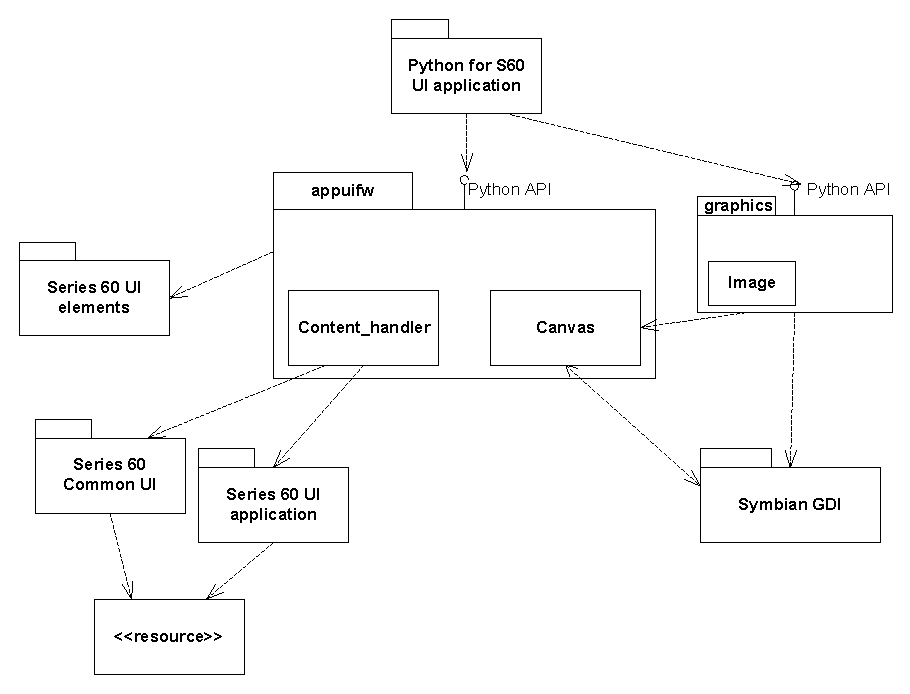
\includegraphics[width=\textwidth]{ui-overview}
\caption{Python for S60 UI environment overview}
\label{fig:ui-overview}
\end{figure}

\subsection{Basics of appuifw Module}
\label{subsec:basics}
Figure \ref{fig:normal-uilayout} shows the layout of a S60 application 
UI in the normal screen mode and a summary of how it relates to the services 
available at the \module{appuifw} API. For alternative layouts, see 
Figure \ref{fig:alternate-uilayouts}.

\begin{figure}
\centering
%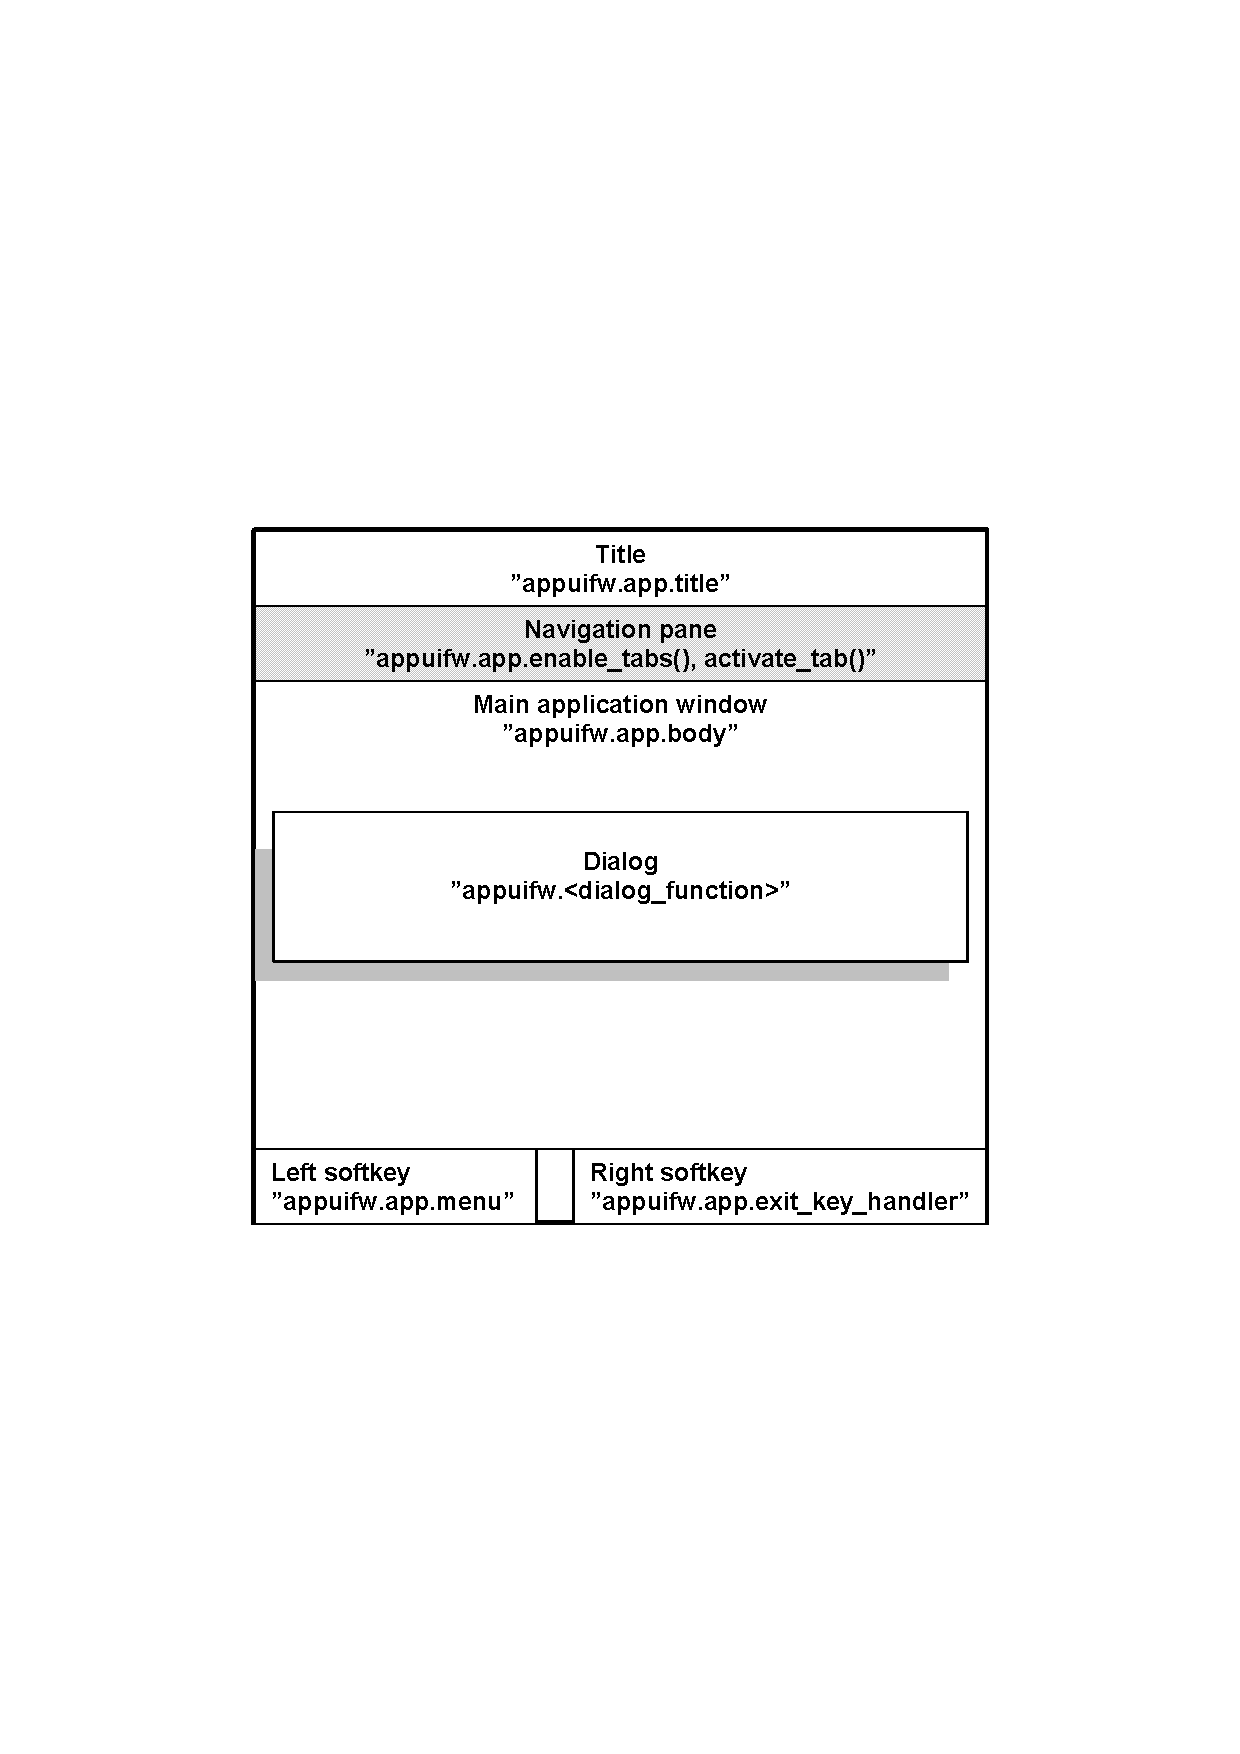
\includegraphics[width=0.7\textwidth]{screen-parts}
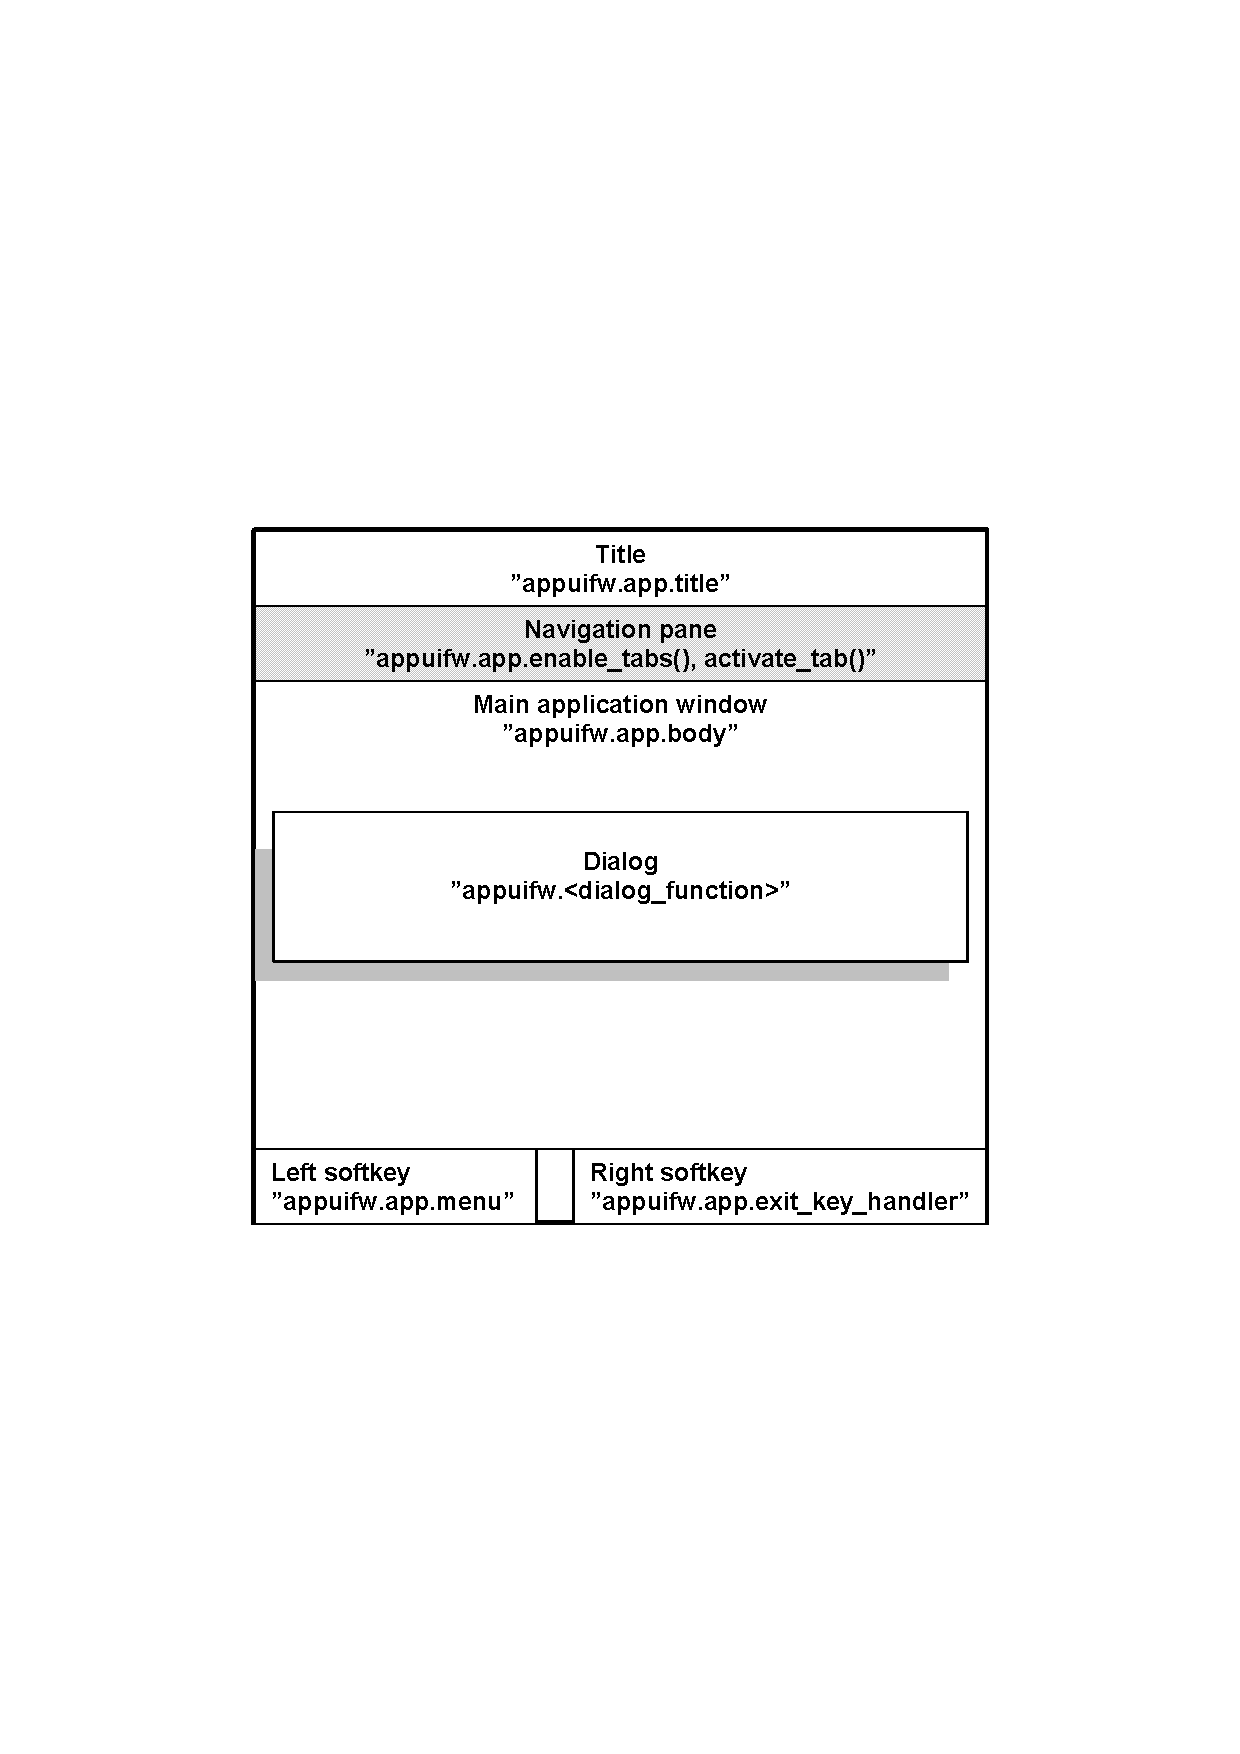
\includegraphics{screen-parts}
\caption{The different parts of the screen when using the 'normal' layout}
\label{fig:normal-uilayout}
\end{figure}

\begin{figure}
\centering
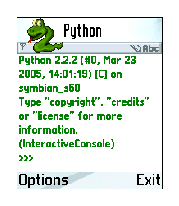
\includegraphics[width=\screenwidth]{layout-normal}
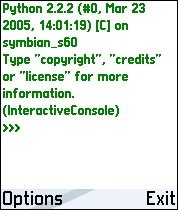
\includegraphics[width=\screenwidth]{layout-large}
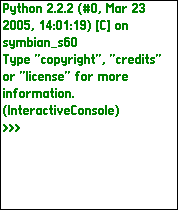
\includegraphics[width=\screenwidth]{layout-full}
\caption{UI layouts. left: 'normal', middle: 'large', right: 'full'}
\label{fig:alternate-uilayouts}
\end{figure}

The main application window may be set up to be occupied by a UI control.

A multi-view application can show the different views as tabs in the 
navigation pane and react as the users navigate between tabs. 

Dialogs always take precedence over the usual UI controls and appear on top 
of them.

UI controls are implemented as Python types. These types are available:

\begin{itemize}
\item \class{Text}
\item \class{Listbox}
\item \class{Canvas}
\end{itemize}
UI controls appear on the screen as soon as an instance of the corresponding 
Python type is set to the body field (\var{app.body}) of the current application UI.

\class{Form} is a versatile dialog implemented as a type.

The \class{Content_handler} type facilitates interfacing to other UI
applications and common high-level UI components. It is based on the
notion that designated handlers can reduce UI application interaction
to operations on MIME-type content.

The following dialogs are implemented as functions:

\begin{itemize}
\item \function{note}
\item \function{query}
\item \function{multi_query}
\item \function{selection_list}
\item \function{multi_selection_list}
\item \function{popup_menu}
\end{itemize}
A dialog becomes visible as soon as the corresponding Python function has 
been called. The function returns with the eventual user input or 
information on the cancellation of the dialog. \class{Form} is an 
exception; it is shown when its \method{execute} method is called.

\subsection{Softkeys}
\label{subsec:softkeys}
The softkeys are managed by the underlying S60 Platform. When no
dialog is visible, the right softkey is bound to application exit and
the left one represents an Options menu. Python for S60 offers
an interface for manipulating the menu and for binding the Exit key to
a Python-callable object (see Section \ref{subsec:application}). 

The native code that implements a dialog also manages the softkeys of the 
dialog, typically OK and Cancel. When the user input needs to be validated 
before accepting it and dismissing the dialog, it is best to use 
\class{Form}.

\subsection{Module Level Functions}
\label{subsec:module}
The following free functions - functions that do not belong to any class 
- are defined in the \module{appuifw} module:

\begin{funcdesc}{available_fonts}{}
Returns a list (Unicode) of all fonts available in the device.
\end{funcdesc}

\begin{funcdesc}{query}{label, type\optional{, initial_value}}
Performs a query with a single-field dialog. The prompt is set to 
\var{label}, and the type of the dialog is defined by \var{type}. The 
value of \var{type} can be any of the following strings:

\begin{itemize}
\item \code{'text'}
\item \code{'code'}
\item \code{'number'}
\item \code{'date'}
\item \code{'time'}
\item \code{'query'}
\item \code{'float'}
\end{itemize}

The type of the optional \var{initial_value} parameter and the 
returned input depend on the value of \var{type}:

\begin{itemize}
\item For text fields, (\code{'text'}, \code{'code'}) it is Unicode
\item For number fields, it is numeric
\item For date fields, it is seconds since epoch rounded down to the nearest local midnight
\end{itemize}

A simple confirmation query and time query take no initial value and return 
\code{True/None} and seconds since local midnight, correspondingly. All 
queries return \code{None} if the users cancel the dialog. 

For \code{'float'} query the \var{initial_value} setting has no 
effect.
\end{funcdesc}


\begin{funcdesc}{multi_query}{label_1, label_2}
A two-field text (Unicode) input dialog. Returns the inputted values
as a 2-tuple. Returns \code{None} if the users cancel the dialog.
\end{funcdesc}

\begin{funcdesc}{note}{text\optional{, type\optional{, global}}}
Displays a note dialog of the chosen type with \var{text} 
(Unicode). The default value for \var{type} is \code{'info'}, which is 
automatically used if \var{type} is not set. \var{type} can be one of 
the following strings: \code{'error'}, \code{'info'}, or 
\code{'conf'}. 

If \var{global} (integer) is any other value than zero a global note is 
displayed. A global note is displayed even if the Python application calling 
this function is in background. The same set of \var{type}s is supported as in 
standard note.
\end{funcdesc}

\begin{funcdesc}{popup_menu}{list\optional{, label}}
A pop-up menu style dialog. \var{list} representing the menu 
contents can be a list of Unicode strings or a list of Unicode string pairs 
(tuples). The resulting dialog list is then a single-style or a double-style 
list. A single-style list is shown in full; whereas a double-style list 
shows the items one at a time. Returns \code{None} if the user cancels the 
operation.
\end{funcdesc}

\begin{funcdesc}{selection_list}{choices\optional{, search_field=0}}
Executes a dialog that allows the users to select a list item and
returns the \var{index} of the chosen item, or \code{None} if the
selection is cancelled by the users. \var{choices} is a list of
Unicode strings.
\var{search_field} is \code{0} (disabled) by default and is optional. Setting it to \code{1} enables a search field (find pane) that facilitates searching for items in long lists. If enabled, the search field appears after you press a letter key.
\end{funcdesc}

\begin{funcdesc}{multi_selection_list}{choices\optional{, style='checkbox', search_field=0}}
  Executes a dialog that allows the users to select multiple list
  items.  Returns a tuple of indexes (a pair of Unicode strings) of
  the chosen items, or empty tuple if the selection is cancelled by
  the users. \var{choices} is a list of Unicode strings.  \var{style}
  is an optional string; the default value being \code{'checkbox'}.
  If \code{'checkbox'} is given, the list will be a checkbox list,
  where empty checkboxes indicate what items can be marked. The other
  possible value that can be set for \var{style} is
  \code{'checkmark'}. If \code{'checkmark'} is given, the list will be
  a markable list, which lists items but does not indicate
  specifically that items can be selected. To select items on a
  markable list, use the Navigation key to browse the list and the
  Edit key to select an item. For example views on checkbox and
  markable lists, see
  \figurename~\ref{fig:checkbox-and-markable-list}.
  \var{search_field} is \code{0} (disabled) by default and is
  optional. Setting it to \code{1} enables a search field (find pane)
  that facilitates searching for items in long lists. If enabled, the
  search field is always visible with checkbox lists; with markable
  lists it appears by pressing a letter key.

Example:
\begin{verbatim}
tuple = appuifw.multi_selection_list(L, style='checkmark', search_field=1)
\end{verbatim}
\end{funcdesc}

\begin{figure}[htbp]
\centering
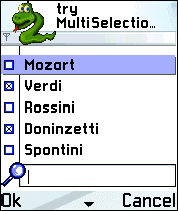
\includegraphics[width=\screenwidth]{checkbox-list}
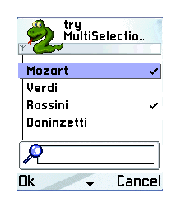
\includegraphics[width=\screenwidth]{markable-list}
\caption{Examples of a checkbox list (left) and a markable list (right)}
\label{fig:checkbox-and-markable-list}
\end{figure}

\subsection{Application Type}
\label{subsec:application}
A single implicit instance of this type always exists when \module{appuifw} 
module is present and can be referred to with the name \code{app}. New 
instances cannot be created by a Python program.

\begin{classdesc*}{Application}
Instances of \class{Application} type have the following attributes:

\begin{memberdesc}[Application]{body}
The UI control that is visible in the application's main window. Currently 
either \class{Text}, a \class{Listbox} object, \class{Canvas}, or 
\code{None}.
\end{memberdesc}

\begin{memberdesc}[Application]{exit_key_handler}
A callable object that is called when the user presses the Exit softkey. 
Setting \member{exit_key_handler} to \code{None} sets it back to the 
default value.
\end{memberdesc}

\begin{memberdesc}[Application]{menu}
This is a list of the following kinds of items:
\begin{itemize}
\item \code{(title, callback)} which creates a regular menu item
\item \code{(title, ((title, callback)\optional{...}))} which creates a submenu
\end{itemize}

\var{title} (Unicode) is the name of the item and \var{callback} the associated callable object. 
The maximum allowed number of items in a menu, or items in a submenu,
or submenus in a menu is 30.

Example:
\begin{verbatim}
appuifw.app.menu = [(u"Item 1", item1),
                    (u"Submenu 1", 
                        ((u"Subitem 1", subitem1),
                         (u"Subitem 2", subitem2)))]
\end{verbatim}
\end{memberdesc}

\begin{memberdesc}[Application]{screen}
The screen area used by an application. See \figurename~\ref{fig:alternate-uilayouts} for
example screens. The appearance of the application on the screen can
be affected by setting one of the following values: \code{'normal'},
\code{'large'}, and \code{'full'}.

Examples:
\begin{verbatim}
appuifw.app.screen='normal' # (a normal screen with title pane and softkeys)
appuifw.app.screen='large'  # (only softkeys visible)
appuifw.app.screen='full'   # (a full screen)
\end{verbatim}
\end{memberdesc}

\begin{memberdesc}[Application]{title}
The title the application that is visible in the application's title
pane. Must be Unicode.
\end{memberdesc}

\begin{memberdesc}[Application]{focus}
A callable object that is called with integer as parameter (0 = focus lost, 
1 = focus regained) when the application receives focus or it is switched to 
background. Focus is received e.g. when the application is switched from 
background to foreground or when the focus is regained from screensaver. 
Similarly when the screensaver is displayed, focus is lost.

Examples:
\begin{verbatim}
>>> import appuifw
>>> def cb(fg):
...   if(fg):
...     print "foreground"
...   else:
...     print "background"
...
>>> appuifw.app.focus=cb
>>> # switch to background, following text is printed from callback:
>>> background
>>> # switch to foreground, following text is printed from callback:
>>> foreground
\end{verbatim}

\begin{notice}
An improper callback can cause adverse effects. If you, for example,
define a callback which takes no parameters you will receive
never-ending \exception{TypeError} exceptions on the Nokia 6600.
\end{notice}

\end{memberdesc}

\begin{memberdesc}[Application]{orientation}
Available only for S60 3rdEd. 
The orientation of the application. The orientation of the application can be 
one of the following values: \code{'automatic'} (this is the default value), 
\code{'portrait'} or \code{'landscape'}.
\end{memberdesc}

Instances of \class{Application} type have the following methods:

\begin{methoddesc}[Application]{activate_tab}{index}
Activates the tab \var{index} counting from zero.
\end{methoddesc}

\begin{methoddesc}[Application]{full_name}{}
Returns the full name, in Unicode, of the native application in whose 
context the current Python interpreter session runs.
\end{methoddesc}

\begin{methoddesc}[Application]{uid}{}
Returns the UID, in Unicode, of the native application in whose 
context the current Python interpreter session runs.
\end{methoddesc}

\begin{methoddesc}[Application]{set_exit}{}
Requests a graceful exit from the application as soon as the current script 
execution returns.
\end{methoddesc}

\begin{methoddesc}[Application]{set_tabs}{tab_texts\optional{,callback=None}}
Sets tabs with given names on them in the navigation bar; 
\var{tab_texts} is a list of Unicode strings. When the users 
navigate between tabs, \var{callback} gets called with the index 
of the active tab as an argument. Tabs can be disabled by giving an empty or 
one-item \var{tab_texts} list.
\end{methoddesc}


\begin{methoddesc}[Application]{layout}{layout_id}

\begin{notice}[note]
Available from S60 2ndEd FP3 onwards (inclusive).
\end{notice}

Returns as a tuple the size and the position of the requested \code{layout_id}. 
The logical layouts are outlined partly in Figure \ref{fig:normal-uilayout}. The 
position is given from the top left corner. The \code{layout_id} can be one of 
the constants defined in module \module{appuifw}\footnote{Descriptions of the 
values are from the S60 SDK documentation \cite{S60Doc}.}:

\begin{datadesc}{EScreen} 
Screen.  
\end{datadesc}

\begin{datadesc}{EApplicationWindow} 
 Window that fills the entire screen.
\end{datadesc}

\begin{datadesc}{EStatusPane} 
Indicates common components for most of the applications.  
\end{datadesc}

\begin{datadesc}{EMainPane} 
The application main pane is used in all the applications.  
\end{datadesc}

\begin{datadesc}{EControlPane} 
Control pane.
\end{datadesc}

\begin{datadesc}{ESignalPane} 
The signal pane is used to indicate signal strength.  
\end{datadesc}

\begin{datadesc}{EContextPane} 
The context pane is used to indicate an active application.
\end{datadesc}

\begin{datadesc}{ETitlePane} 
Used to indicate the subject or the name of the main pane content. 
\end{datadesc}

\begin{datadesc}{EBatteryPane} 
The battery pane is used to indicate battery strength.  
\end{datadesc}

\begin{datadesc}{EUniversalIndicatorPane} 
The universal indicator pane is used to indicate items that require the user's 
attention while browsing applications. 
\end{datadesc}

\begin{datadesc}{ENaviPane} 
The navi pane is used to indicate navigation within an application, to provide 
context sensitive information to the user while entering or editing data, or to 
show additional information.  
\end{datadesc}

\begin{datadesc}{EFindPane} 
A fixed find pane is used with lists instead of the find pop-up window.  
\end{datadesc}

\begin{datadesc}{EWallpaperPane} 
Wallpaper pane.  
\end{datadesc}

\begin{datadesc}{EIndicatorPane} 
The universal indicator pane is used to indicate items that require the user's 
attention while browsing applications.  
\end{datadesc}

\begin{datadesc}{EAColumn} 
Used generally to display small sized graphics or heading texts.  
\end{datadesc}

\begin{datadesc}{EBColumn} 
Used generally to display large sized icons or heading texts.  
\end{datadesc}

\begin{datadesc}{ECColumn} 
Used generally to display data entered by the user. Overlaps with the D column. 
\end{datadesc}

\begin{datadesc}{EDColumn} 
Used generally to display additional icons. Overlaps with the C column. 
\end{datadesc}

\begin{datadesc}{EStaconTop} 
Top part of status and control panes in landscape layout.  
\end{datadesc}

\begin{datadesc}{EStaconBottom} 
Bottom part of status and control panes in landscape layout.  
\end{datadesc}

\begin{datadesc}{EStatusPaneBottom} 
Bottom part of status pane in landscape layout.  
\end{datadesc}

\begin{datadesc}{EControlPaneBottom} 
Bottom part of control pane in landscape layout.  
\end{datadesc}

\begin{datadesc}{EControlPaneTop} 
Top part of control pane in landscape layout.  
\end{datadesc}

\begin{datadesc}{EStatusPaneTop} 
Top part of status pane in landscape layout.
\end{datadesc}

Example:
\begin{verbatim}
>>> import appuifw
>>> appuifw.app.layout(appuifw.EMainPane)
((176, 144), (0, 44))
>>> # size and position (x, y) of the main pane in Nokia N70
\end{verbatim}

\end{methoddesc}

\end{classdesc*}

\subsection{Form Type}
\label{subsec:form}
\class{Form} implements a dynamically configurable, editable multi-field 
dialog. \class{Form} caters for advanced dialog use cases with requirements 
such as free selectability of the combination of fields, possibility of 
validating the user input, and automatically producing the contents of some 
dialog fields before allowing the closing of the dialog. 

\begin{classdesc}{Form}{fields\optional{, flags=0}}
Creates a \class{Form} instance.
\var{fields} is a list of \emph{field descriptors}: \code{(label, type\optional{, value})} where

\var{label} is a Unicode string

\var{type} is one of the following strings: 
\code{'text'}, \code{'number'}, \code{'date'}, \code{'time'}, \code{'combo'}
or \code{'float'}

\var{value}, depending on \var{type}: Unicode string, numeric, float (seconds 
since Unix epoch rounded down to the nearest local midnight), float (seconds 
since local midnight), \code{([choice_label ...], index)} of float. For 
\code{'float'} \var{type} the initial value setting might not be shown in the 
UI.
\end{classdesc}

\class{Form} can also be configured and populated after construction. The 
configuration flags are visible as an attribute. \class{Form} implements 
the list protocol that can be used for setting the form fields, as well as 
obtaining their values after the dialog has been executed.

Instances of \class{Form} type have the following attributes:

\begin{memberdesc}[Form]{flags}
This attribute holds the values of the various configuration flags. 
Currently supported flags are:

\begin{datadesc}{FFormEditModeOnly}
When this flag is set, the form remains in edit mode while \method{execute} 
runs.
\end{datadesc}

\begin{datadesc}{FFormViewModeOnly}
When this flag is set, the form cannot be edited at all.
\end{datadesc}

\begin{datadesc}{FFormAutoLabelEdit}
This flag enables support for allowing the end-users to edit the labels of 
the form fields.
\end{datadesc}

\begin{datadesc}{FFormAutoFormEdit}
This flag enables automatic support for allowing the end-users to add and 
delete the form fields. Note that this is an experimental feature and is not 
guaranteed to work with all SDK versions.
\end{datadesc}

\begin{datadesc}{FFormDoubleSpaced}
When this flag is set, double-spaced layout is applied when the form is 
executed: one field takes two lines, as the label and the value field are on 
different lines.
\end{datadesc}
\end{memberdesc}

\begin{memberdesc}[Form]{menu}
A list of \code{(title, callback)} pairs, where 
each pair describes an item in the form's menu bar that is active while the 
dialog is being executed. \var{title} (Unicode) is the name of 
the item and \var{callback} the associated callable object.
\end{memberdesc}

\begin{memberdesc}[Form]{save_hook}
This attribute can be set to a callable object that receives one argument 
and returns a Boolean value. It gets called every time the users want to 
save the contents of an executing \class{Form} dialog. A candidate list for 
new form content - a list representing the currently visible state of the 
UI - is given as an argument. The list can be modified by 
\member{save_hook}. If \member{save_hook} returns \code{True}, the 
candidate list is set as the new contents of the form. Otherwise, the form 
UI is reset to reflect the field list contained in \class{Form} object.
\end{memberdesc}

Instances of \class{Form} type have the following methods:

\begin{methoddesc}[Form]{execute}{}
Executes the dialog by making it visible on the UI.
\end{methoddesc}

\begin{methoddesc}[Form]{insert}{index, field_descriptor}
Inserts the field descriptor into the \class{Form} before the given \var{index}.
\end{methoddesc}

\begin{methoddesc}[Form]{pop}{}
Removes the last field descriptor from the \class{Form} and returns it.
\end{methoddesc}

\begin{methoddesc}[Form]{length}{}the number of field descriptors in the form.
\end{methoddesc}

The subscript notation \code{f[i]} can be used to access or modify the
i-th element of the form \code{f}. Same limitations as discussed above
in the context of the flag \constant{FFormAutoFormEdit} apply to
modifying a form while it is executing. The ability to change the
schema of a form while it is executing is an experimental feature.

\subsection{Text Type}
\label{subsec:mylabel5}
\class{Text} is a text editor UI control. For examples on the options 
available with \class{Text}, see Figure \ref{fig:text-styles}.

\begin{figure}[htbp]
\centering
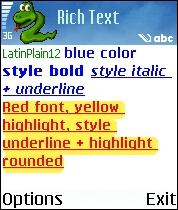
\includegraphics[width=\screenwidth]{text-styles-1}
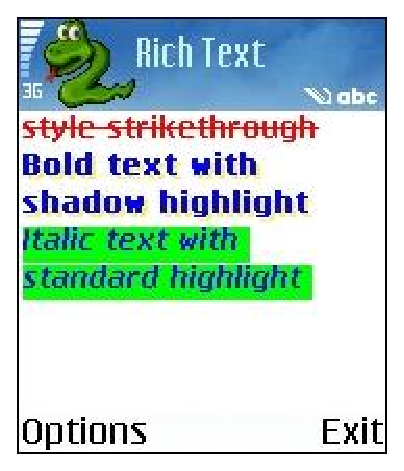
\includegraphics[width=\screenwidth]{text-styles-2}
\caption{Examples of the options available for Text type}
\label{fig:text-styles}
\end{figure}

Instances of \class{Text} type have the following attributes:

\begin{memberdesc}[Text]{color}
The color of the text. \code{color} supports the same color representation 
models as the \module{graphics} module. For the supported color 
representation models, see Section \ref{sec:graphics}.
\end{memberdesc}

\begin{memberdesc}[Text]{focus}
A Boolean attribute that indicates the focus state of the control. Editor 
control also takes the ownership of the navigation bar, and this feature is 
needed to enable the usage of this control in applications that use the 
navigation bar - for example, navigation tabs.
\end{memberdesc}

\begin{memberdesc}[Text]{font} 
The font of the text. There are two possible ways to set this attribute:

\begin{itemize}

\item Using a supported Unicode font, for example \code{u"Latin12"}. Trying to set a font which is not supported by the device has no effect. A list of supported fonts can be retrieved by using \function{appuifw.available_fonts}.

Example, setting font:
\begin{verbatim}
t = appuifw.Text()
t.font = u"albi17b" # sets font to Albi 17 bold
t.font = u"LatinPlain12" # sets font to Latin Plain 12
\end{verbatim}
\item Using one of the default device fonts that are associated with the following labels (plain strings):
\code{'annotation', 'title', 'legend', 'symbol', 'dense', 'normal'}
Example, setting font: 
\begin{verbatim}
t.font = "title" # sets font to the one used in titles
\end{verbatim}

Example, checking the currently set font: 
\begin{verbatim}
unicodeFont = t.font
\end{verbatim}
\end{itemize}

The attribute value retrieved is always a Unicode string. If the font has 
been set with a label, for example, \code{'title'}, the attribute will 
retrieve the font associated with that label. 
\end{memberdesc}

\begin{memberdesc}[Text]{highlight_color}
The highlight color of the text. \code{highlight_color} supports the 
same color representation models as the \module{graphics} module. For the 
supported color representation models, see Section \ref{sec:graphics}.
\end{memberdesc}

\begin{memberdesc}[Text]{style}
The style of the text. The flags for this attribute are defined in the 
\module{appuifw} module. These flags can be combined by using the binary 
operator \code{|}. The flags can be divided into two types: text style 
and text highlight. Text style flags can be freely combined with each other. 
However, one or more text style flags can be combined with only one text 
highlight flag. The flags are:

Text style:

\begin{datadesc}{STYLE_BOLD} 
Enables bold text.
\end{datadesc}

\begin{datadesc}{STYLE_UNDERLINE}
Enables underlined text.
\end{datadesc}

\begin{datadesc}{STYLE_ITALIC} 
Enables italic text.
\end{datadesc}

\begin{datadesc}{STYLE_STRIKETHROUGH } 
Enables strikethrough.
\end{datadesc}

Text highlight:

\begin{datadesc}{HIGHLIGHT_STANDARD}
Enables standard highlight.
\end{datadesc}

\begin{datadesc}{HIGHLIGHT_ROUNDED}
Enables rounded highlight.
\end{datadesc}

\begin{datadesc}{HIGHLIGHT_SHADOW}
Enables shadow highlight.
\end{datadesc}

Only one highlight is allowed to be used at once. Therefore, it is possible 
to combine only one highlight with one or more text styles.

Examples:
\begin{verbatim}
t = appuifw.Text()

# These and other similar values and combinations are valid:
t.style = appuifw.STYLE_BOLD
t.style = appuifw.STYLE_UNDERLINE
t.style = appuifw.STYLE_ITALIC
t.style = appuifw.STYLE_STRIKETHROUGH
t.style = (appuifw.STYLE_BOLD|
	   appuifw.STYLE_ITALIC|
	   appuifw.STYLE_UNDERLINE)

# These values are valid:
t.style = appuifw.HIGHLIGHT_STANDARD
t.style = appuifw.HIGHLIGHT_ROUNDED
t.style = appuifw.HIGHLIGHT_SHADOW

# This combination is NOT valid:
# Invalid code, do not try!
t.style = (appuifw.HIGHLIGHT_SHADOW|appuifw.HIGHLIGHT_ROUNDED)
\end{verbatim}
\end{memberdesc}

Instances of \class{Text} type have the following methods:

\begin{methoddesc}[Text]{add}{text}
Inserts the Unicode string \var{text} to the current cursor position.
\end{methoddesc}

\begin{methoddesc}[Text]{bind}{event_code, callback}
Binds the callable Python object \var{callback} to event
\var{event_code}. The key codes are defined in 
the \module{key_codes} library module. The call 
\code{bind(event_code, None)} clears an 
existing binding. In the current implementation the event is always
passed also to the underlying native UI control.
\end{methoddesc}

\begin{methoddesc}[Text]{clear}{}
Clears the editor.
\end{methoddesc}

\begin{methoddesc}[Text]{delete}{\optional{pos=0, length=len()}}
Deletes \var{length} characters of the text held by the editor control, 
starting from the position \var{pos}.
\end{methoddesc}

\begin{methoddesc}[Text]{get_pos}{}
Returns the current cursor position.
\end{methoddesc}

\begin{methoddesc}[Text]{len}{}
Returns the length of the text string held by the editor control.
\end{methoddesc}

\begin{methoddesc}[Text]{get}{\optional{pos=0, length=len()}}
Retrieves \code{length} characters of the text held by the editor control, 
starting from the position \var{pos}.
\end{methoddesc}

\begin{methoddesc}[Text]{set}{text}
Sets the text content of the editor control to Unicode string 
\var{text}.
\end{methoddesc}

\begin{methoddesc}[Text]{set_pos}{cursor_pos}
Sets the cursor to \var{cursor_pos}.
\end{methoddesc}

\subsection{Listbox Type}
\label{subsec:listbox}

\begin{figure}[htbp]
\centering
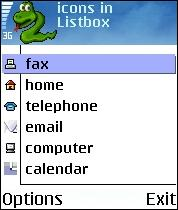
\includegraphics[width=\screenwidth]{listbox-with-icons}
\caption{Listbox with icons}
\label{fig:listbox-with-icons}
\end{figure}

An instance of this UI control type is visible as a listbox, also known as a 
list in Symbian, that can be configured to be a single-line item or a 
double-item listbox. Figure \ref{fig:listbox-with-icons} shows a single-line 
item Listbox with icons. For more information on the MBM and MIF formats, 
see Section \ref{subsec:icon}.

\begin{classdesc}{Listbox}{list, callback}
Creates a \class{Listbox} instance. A callable object 
\var{callback} gets called when a listbox selection has been 
made. \code{list} defines the content of the listbox and can be one of the 
following:

\begin{itemize}
\item A normal (single-line item) listbox: a list of Unicode strings, for example \code{[unicode_string item1, unicode_string item2]}
\item A double-item listbox: a two-element tuple of Unicode strings , for example \code{[(unicode_string item1, unicode_string item1description), (unicode_string item2, unicode_string item2description)]}
\item A normal (single-line item) listbox with graphics: a two-element tuple consisting of a Unicode string and an \class{Icon} object, for example \code{[(unicode_string item1, icon1), (unicode_string item2, icon2)]}.
\item A double-item listbox with graphics: a three-element tuple consisting of two Unicode strings and one \class{Icon} object, for example \code{[(unicode_string item1, unicode_string item1description, icon1), (unicode_string item2, unicode_string item2description, icon2)]}
\end{itemize}

Example: To produce a normal (single-line item) listbox with graphics:
\begin{verbatim}
icon1 = appuifw.Icon(u"z:\\system\\data\\avkon.mbm", 28, 29)
icon2 = appuifw.Icon(u"z:\\system\\data\\avkon.mbm", 40, 41)
entries = [(u"Signal", icon1),
           (u"Battery", icon2)]
lb = appuifw.Listbox(entries, lbox_observe)
\end{verbatim}
\end{classdesc}

Instances of \class{Listbox} type have the following methods:

\begin{methoddesc}[Listbox]{bind}{event_code, callback}
Binds the callable Python object \var{callback} to event 
\var{event_code}. The key codes are defined in 
the \module{key_codes} library module. The call
\code{bind(event_code, None)} clears an 
existing binding. In the current implementation the event is always passed 
also to the underlying native UI control.
\end{methoddesc}

\begin{methoddesc}[Listbox]{current}{}
Returns the currently selected item's index in the \class{Listbox}.
\end{methoddesc}

\begin{methoddesc}[Listbox]{set_list}{list\optional{, current}}
Sets the \class{Listbox} content to a list of Unicode strings or a
list of tuples of Unicode strings. The accepted structures of \var{list} are the
same as in the \class{Listbox} constructor. The optional argument \var{current} is the index of the focused list item.
\end{methoddesc}

\subsection{Icon Type}
\label{subsec:icon}
An instance of \class{Icon} type encapsulates an icon to be used together 
with a \class{Listbox} instance. Note that currently \class{Icon} can only 
be used with \class{Listbox} (see Section \ref{subsec:listbox}).

MBM is the native Symbian OS format used for pictures. It is a
compressed file format where the files can contain several bitmaps and
can be referred to by a number. An \code{.mbg} file is the header file
usually associated with an \code{.mbm} file, which includes symbolic
definitions for each bitmap in the file. For example, an
\file{avkon.mbm} file has an associated index file called
\file{avkon.mbg}, which is included in S60 SDKs. For more information
on the MBM format and the bitmap converter tool, see \cite{S60Doc} and
search the topics with the key term "How to provide Icons"; this topic
also points you to the Bitmap Converter tool that can be used for
converting bitmaps into the MBM format.

S60 2$^{nd}$ Edition FP3 introduces a new format for icons called 
Multi-Image File (MIF). This format is very similar to the MBM format and 
also contains several compressed files. The files to be compressed should be 
in Scalable Vector Graphics Tiny (SVG-T) format. For more information on the 
SVG format, see Scalable Vector Graphics (SVG) 1.1 Specification 
[10].

\begin{classdesc}{Icon}{filename, bitmap, bitmapMask}
Creates an icon. \var{filename} is a Unicode file name and must 
include the whole path. Note that MBM and MIF (MIF only in S60 2nd 
Edition FP3) are the only file formats supported. \var{bitmap} 
and \var{bitmapMask} are integers that represent the index of 
the icon and icon mask inside that file respectively.
\end{classdesc}

Example: The following builds an icon with the standard signal symbol:
\begin{verbatim}
icon = appuifw.Icon(u"z:\\system\\data\\avkon.mbm", 28, 29)
\end{verbatim}

\subsection{Content_handler Type}
\label{subsec:content}

An instance of \class{Content_handler} handles data content by its MIME 
type.

\begin{classdesc}{Content_handler}{\optional{callback}}
Creates a \class{Content_handler} instance. A Content_handler handles
data content by its MIME type. The optional
\var{callback} is called when the embedded handler application 
started with the \method{open} method finishes. 
\end{classdesc}

Instances of \class{Content_handler} type have the following methods:

\begin{methoddesc}[Content_handler]{open}{filename}
Opens the file \var{filename} (Unicode) in its handler 
application if one has been registered for the particular MIME type. The 
handler application is embedded in the caller's thread. The call to this 
function returns immediately. When the handler application finishes, the 
\var{callback} that was given to the \class{Content_handler} 
constructor is called.
\end{methoddesc}

\begin{methoddesc}[Content_handler]{open_standalone}{filename}
Opens the file \var{filename} (Unicode) in its handler 
application if one has been registered for the particular MIME type. The 
handler application is started in its own process. The call to this function 
returns immediately. Note that \var{callback} is not called for 
applications started with this method.
\end{methoddesc}

\subsection{Canvas Type}
\label{subsec:canvas}
\class{Canvas} is a UI control that provides a drawable area on the screen 
and support for handling raw key events. \class{Canvas} supports the 
standard drawing methods that are documented in Section \ref{sec:graphics}.

\begin{classdesc}{Canvas}{\optional{redraw_callback=None, event_callback=None,
                                  resize_callback=None}}
Constructs a \class{Canvas}. The optional parameters are callbacks
that are called when specific events occur. 

\note{Watch out for cyclic
references here. For example, if the callbacks are methods of an
object that holds a reference to the \class{Canvas}, a reference cycle
is formed that must be broken at cleanup time or the
\class{Canvas} will not be freed.}

\var{redraw_callback} is called whenever a part of the \class{Canvas} 
has been obscured by something, is then revealed, and needs to be
redrawn. This can typically happen, for example, when the user
switches away from the Python application and back again, or after
displaying a pop-up menu. The callback takes as its argument a
four-element tuple that contains the top-left and the bottom-right
corner of the area that needs to be redrawn. In many cases redrawing
the whole
\class{Canvas} is a reasonable option. 

\var{event_callback} is called whenever a raw key event is received.
There are three kinds of key events: \code{EEventKeyDown},
\code{EEventKey}, and \code{EEventKeyUp}. When a user presses a key 
down, events \code{EEventKeyDown} and \code{EEventKey} are generated. 
When the key is released, an \code{EEventKeyUp} event is generated.

The argument to the \var{event_callback} is a dictionary that contains 
the following data for key events:

\begin{itemize}
\item \code{'type'}: one of \code{EEventKeyDown}, \code{EEventKey}, or \code{EEventKeyUp}
\item \code{'keycode'}: the keycode of the key
\item \code{'scancode'}: the scancode of the key
\item \code{'modifiers'}: the modifiers that apply to this key event
\end{itemize}

Each key on the keyboard has one or more scancodes and zero or more keycodes 
associated with it. A scancode represents the physical key itself and a 
keycode is the result of state-related operating system defined processing 
done on the key. For keys that correspond to a symbol in the current 
character set of the phone, the keycode is equal to the code of the 
corresponding symbol in that character set. For example, if you are using 
the Nokia Wireless Keyboard (SU-8W), pressing the key A will always produce 
the scancode 65 (ASCII code for an upper case A), but the keycode 
could be either 65 or 91 (ASCII code for a lower case A) depending on 
whether or not the Shift key is pressed or Caps Lock is active. 

The \module{key_codes} module contains definitions for the keycodes and 
scancodes. See \figurename~\ref{fig:keyboard} for the codes of the most 
common keys on the phone keypad. 

Some keys are handled in a special way:

\begin{itemize}
\item A short press of the Edit key causes it to stay down, meaning that no \code{EEventKeyUp} event is sent. The event is only sent after a long press.
\item Detecting presses of the Voice tags key or the Power key is not supported.
\item If the right softkey is pressed, the \code{appuifw.app.exit_key_handler} callback is always executed.
\end{itemize}

There is no way to prevent the standard action of the Hang-up key, the Menu 
key, the Power key or the Voice tags key from taking place.

\begin{figure}
\centering
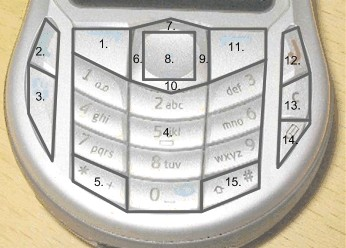
\includegraphics[width=5in]{6630keyboard}
%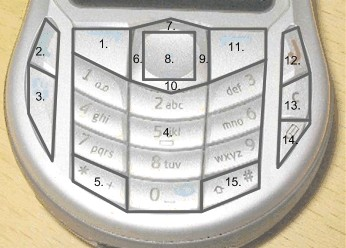
\includegraphics[width=3.60in,height=2.58in]{6630keyboard}
%\centerline{\includegraphics[width=3.60in,height=2.58in]{API_Reference_for_Python11.eps}} \par & 
\begin{tableiii}{lll}{textrm}{Key}{Keycode}{Scancode}
\lineiii{1.}{EKeyLeftSoftkey}{EScancodeLeftSoftkey}
\lineiii{2.}{EKeyYes}{EScancodeYes}
\lineiii{3.}{EKeyMenu}{EScancodeMenu}
\lineiii{4.}{EKey0...9}{EScancode0...9}
\lineiii{5.}{EKeyStar}{EScancodeStar}
\lineiii{6.}{EKeyLeftArrow}{EScancodeLeftArrow}
\lineiii{7.}{EKeyUpArrow}{EScancodeUpArrow}
\lineiii{8.}{EKeySelect}{EScancodeSelect}
\lineiii{9.}{EKeyRightArrow}{EScancodeRightArrow}
\lineiii{10.}{EKeyDownArrow}{EScancodeDownArrow}
\lineiii{11.}{EKeyRightSoftkey}{EScancodeRightSoftkey}
\lineiii{12.}{EKeyNo}{EScancodeNo}
\lineiii{13.}{EKeyBackspace}{EScancodeBackspace}
\lineiii{14.}{EKeyEdit}{EScancodeEdit}
\lineiii{15.}{EKeyHash}{EScancodeHash}
\end{tableiii}
\caption{Keycodes and scancodes for phone keys usable from Python applications}
\label{fig:keyboard}
\end{figure}

\var{resize_callback} is called when screen size is changed when the 
\class{Canvas} rect size has been changed. The callback takes as its argument a
two-element tuple that contains the new clientRect width and height. 

\end{classdesc}

Instances of \class{Canvas} type have the following attribute:

\begin{memberdesc}[Canvas]{size}
A two-element tuple that contains the current width and height of the 
\class{Canvas} as integers.
\end{memberdesc}

Instances of \class{Canvas} type have the same standard drawing methods 
that are documented in Section \ref{sec:graphics}.

% Copyright (c) 2005-2007 Nokia Corporation
%
% Licensed under the Apache License, Version 2.0 (the "License");
% you may not use this file except in compliance with the License.
% You may obtain a copy of the License at
%
%     http://www.apache.org/licenses/LICENSE-2.0
%
% Unless required by applicable law or agreed to in writing, software
% distributed under the License is distributed on an "AS IS" BASIS,
% WITHOUT WARRANTIES OR CONDITIONS OF ANY KIND, either express or implied.
% See the License for the specific language governing permissions and
% limitations under the License.

\newcommand{\notinfirsted}{
\begin{notice}
Not supported in S60 1st Edition!
\end{notice}

}

\section{\module{graphics} ---
  A graphics related services package}
\label{sec:graphics}

\declaremodule{extension}{graphics}
\platform{S60}
\modulesynopsis{A graphics related services package.}

The \module{graphics} module provides access to the graphics primitives and 
image loading, saving, resizing, and transformation capabilities provided by 
the Symbian OS. 

The module is usable from both graphical Python applications and
background Python processes. However, background processes have some
restrictions, namely that plain string symbolic font names are not
supported in background processes since background processes have no
access to the UI framework (see also Section
\ref{subsubsec:font-specs}).

For an example on using this module, see \cite{PyS60Prog}.

Functions \function{Image.open} and \function{Image.inspect} and \class{Image} 
object methods \method{load}, \method{save}, \method{resize}, and 
\method{transpose} are not available for S60 1st Edition.

\subsection{Module Level Functions}
\label{subsec:mylabel7}
The following free functions - functions that do not belong to any class 
- are defined in the \module{graphics} module:

\begin{funcdesc}{screenshot}{}
Takes a screen shot and returns the image in \class{Image} format.
\end{funcdesc}

\subsection{Image Class Static Methods}
\label{subsec:image}
The following \class{Image} class static methods are defined in the 
\module{graphics} module:

\begin{funcdesc}{Image.new}{size\optional{, mode='RGB16'}}
Creates and returns a new \class{Image} object with the given size and 
mode. \var{size} is a two-element tuple. \var{mode} specifies the 
color mode of the \class{Image} to be created. It can be one of the 
following:

\begin{itemize}
\item \code{'1'}: Black and white (1 bit per pixel)
\item \code{'L'}: 256 gray shades (8 bits per pixel)
\item \code{'RGB12'}: 4096 colors (12 bits per pixel)
\item \code{'RGB16'}: 65536 colors (16 bits per pixel)
\item \code{'RGB'}: 16.7 million colors (24 bits per pixel)
\end{itemize}
\end{funcdesc}

\begin{funcdesc}{Image.open}{filename}
\notinfirsted
Returns a new \class{Image} object (mode \code{RGB16}) that contains the 
contents of the named file. The supported file formats are JPEG and PNG. The 
file format is automatically detected based on file contents. 
\var{filename} should be a full path name.
\end{funcdesc}

\begin{funcdesc}{Image.inspect}{filename}
\notinfirsted
Examines the given file and returns a dictionary of the attributes of the 
file. At present the dictionary contains only the image size in pixels as a 
two-element tuple, indexed by key \code{'size'}. 
\var{filename} should be a full path name.
\end{funcdesc}

\subsection{Image Objects}
\label{subsec:image-objects}
An \class{Image} object encapsulates an in-memory bitmap. 

Note on asynchronous methods: Methods \method{resize}, \method{transpose}, 
\method{save}, and \method{load} have an optional callback argument. If the 
callback is not given, the method call is synchronous; when the method
returns, the operation is complete or an exception has been raised. If
the callback is given, the method calls are asynchronous. If all
parameters are valid and the operation can start, the method call will
return immediately.  The actual computation then proceeds in the
background. When it is finished, the callback is called with an error
code as the argument. If the given code is \code{0}, the operation
completed without errors, otherwise an error occurred.

It is legal to use an unfinished image as a source in a blit operation; this 
will use the image data as it is at the moment the blit is made and may thus 
show an incomplete result.

\class{Image} objects have the following methods:

\begin{methoddesc}[Image]{resize}{newsize\optional{, callback=None, keepaspect=0}}
\notinfirsted
Returns a new image that contains a resized copy of this image. If 
\var{keepaspect} is set to \code{1}, the resize will maintain the 
aspect ratio of the image, otherwise the new image will be exactly the given 
size. 

If \var{callback} is given, the operation is asynchronous, and the 
returned image will be only partially complete until \var{callback} is 
called.
\end{methoddesc}

\begin{methoddesc}[Image]{transpose}{direction\optional{, callback=None}}
\notinfirsted

Creates a new image that contains a transformed copy of this image. The 
\var{direction} parameter can be one of the following:

\begin{itemize}
\item \code{FLIP_LEFT_RIGHT}: Flips the image horizontally, exchanging left and right edges.
\item \code{FLIP_TOP_BOTTOM}: Flips the image vertically, exchanging top and bottom edges.
\item \code{ROTATE_90}: Rotates the image 90 degrees counterclockwise.
\item \code{ROTATE_180}: Rotates the image 180 degrees.
\item \code{ROTATE_270}: Rotates the image 270 degrees counterclockwise.
\end{itemize}

If \var{callback} is given, the operation is asynchronous and the 
returned image will be only partially complete until \var{callback} is 
called.
\end{methoddesc}

\begin{methoddesc}[Image]{load}{filename\optional{, callback=None}}
\notinfirsted
Replaces the contents of this \class{Image} with the contents of the named 
file, while keeping the current image mode. This \class{Image} object must 
be of the same size as the file to be loaded.

If \var{callback} is given, the operation is asynchronous and the loaded 
image will be only partially complete until \var{callback} is called. 
\var{filename} should be a full path name.
\end{methoddesc}

\begin{methoddesc}[Image]{save}{filename\optional{,callback=None, format=None, quality=75, bpp=24, compression='default'}}
\notinfirsted
Saves the image into the given file. The supported formats are JPEG and PNG. 
If \var{format} is not given or is set to \code{None}, the format is 
determined based on the file name extension: \code{'.jpg'} or 
\code{'.jpeg'} are interpreted to be in JPEG format and \code{'.png'} to 
be in PNG format. \var{filename} should be a full path name.

When saving in JPEG format, the \var{quality} argument specifies the 
quality to be used and can range from 1 to 100. 

When saving in PNG format, the \var{bpp} argument specifies how many bits 
per pixel the resulting file should have, and \var{compression} specifies 
the compression level to be used. 

Valid values for \var{bpp} are:

\begin{itemize}
\item \code{1}: Black and white, 1 bit per pixel
\item \code{8}: 256 gray shades, 8 bits per pixel
\item \code{24}: 16.7 million colors, 24 bits per pixel
\end{itemize}

Valid values for \var{compression} are:

\begin{itemize}
\item \code{'best'}: The highest possible compression ratio, the slowest speed
\item \code{'fast'}: The fastest possible saving, moderate compression
\item \code{'no'}: No compression, very large file size
\item \code{'default'}: Default compression, a compromise between file size and speed 
\end{itemize}

If \var{callback} is given, the operation is asynchronous. When the 
saving is complete, the \var{callback} is called with the result code.
\end{methoddesc}


\begin{methoddesc}[Image]{stop}{}
Stops the current asynchronous operation, if any. If an asynchronous call is 
not in progress, this method has no effect.
\end{methoddesc}

\class{Image} objects have the following attribute:

\begin{memberdesc}[Image]{size}
A two-element tuple that contains the size of the \class{Image}. Read-only.
\end{memberdesc}

\subsection{Common Features of Drawable Objects}
\label{subsec:common}
Objects that represent a surface that can be drawn on support a set of 
common drawing methods, described in this section. At present there are two 
such objects: \class{Canvas} from the \refmodule{appuifw} module and 
\class{Image} from the \module{graphics} module. 

\subsubsection{Options}
\label{subsubsec:options}
Many of these methods support a set of standard options. This set of options 
is as follows:

\begin{itemize}
\item \var{outline}: The color to be used for drawing outlines of primitives and text. If \code{None}, the outlines of primitives are not drawn.
\item \var{fill}: The color to be used for filling the insides of primitives. If \code{None}, the insides of primitives are not drawn. If \var{pattern} is also specified, \var{fill} specifies the color to be used for areas where the pattern is white.
\item \var{width}: The line width to be used for drawing the outlines of primitives.
\item \var{pattern}: Specifies the pattern to be used for filling the insides of primitives. If given, this must be either \code{None} or a 1-bit (black and white) \class{Image}.
\end{itemize}

\subsubsection{Coordinate representation}
\label{subsubsec:coordinate}
The methods accept an ordered set of coordinates in the form of a coordinate 
sequence. Coordinates can be of type \code{int}, \code{long}, or 
\code{float}. A valid coordinate sequence is a non-empty sequence of 
either

\begin{itemize}
\item Alternating x and y coordinates. In this case the sequence length must be even, or
\item Sequences of two elements, that specify x and y coordinates.
\end{itemize}
Examples of valid coordinate sequences:

\begin{itemize}
\item \code{(1, 221L, 3, 4, 5.85, -3)}: A sequence of three coordinates
\item \code{[(1,221L),(3,4),[5.12,6])}: A sequence of three coordinates
\item \code{(1,5)}: A sequence of one coordinate
\item \code{[(1,5)]}: A sequence of one coordinate
\item \code{[[1,5]]}: A sequence of one coordinate
\end{itemize}

Examples of invalid coordinate sequences:

\textbf{Invalid code, do not use!}
\begin{itemize}
\item \code{[]}: An empty sequence
\item \code{(1,2,3)}: Odd number of elements in a flat sequence
\item \code{[(1,2),(3,4),None]}: Contains an invalid element
\item \code{([1,2],3,4)}: Mixing the flat and nested form is not allowed
\end{itemize}

\subsubsection{Color representation}
\label{subsubsec:color}
All methods that take color arguments accept the following two color 
representations:

\begin{itemize}
\item A three-element tuple of integers in the range from 0 to 255 inclusive, representing the red, green, and blue components of the color.
\item An integer of the form \code{0xrrggbb}, where \code{rr} is the red, \code{gg} the green, and \code{bb} the blue component of the color. 
\end{itemize}
For 12 and 16 bit color modes the color component values are simply 
truncated to the lower bit depth. For the 8-bit grayscale mode images the 
color is converted into grayscale using the formula \code{(2*r+5*g+b)/8}, rounded 
down to the nearest integer. For 1-bit black and white mode images the color 
is converted into black (0) or white (1) using the formula \code{(2*r+5*g+b)/1024}.

Examples of valid colors:

\begin{itemize}
\item \code{0xffff00}: Bright yellow
\item \code{0x004000}: Dark green
\item \code{(255,0,0)}: Bright red
\item \code{0}: Black
\item \code{255}: Bright blue
\item \code{(128,128,128)}: Medium gray
\end{itemize}

Examples of invalid colors:

\textbf{Invalid code, do not use!}
\begin{itemize}
\item \code{(0,0.5,0.9)}: Floats are not supported
\item \code{'{\#}ff80c0'}: The HTML color format is not supported
\item \code{(-1,0,1000)}: Out-of-range values
\item \code{(1,2)}: The sequence is too short
\item \code{[128,128,192]}: This is not a tuple
\end{itemize}

\subsubsection{Font specifications}
\label{subsubsec:font-specs}
A font can be specified in three ways: 
\begin{itemize}
\item None, meaning the default font
\item a Unicode string that represents a full font name, such as \code{u'LatinBold19'}
\item a plain string symbolic name that refers to a font setting currently specified by 
the UI framework
\item as a two or three element tuple, where 
\begin{itemize}
\item the first element is the font name (unicode or string) or None for default font
\item the second element is the font height in pixels or None for default size
\item the third (optional) element is the flags applied to the font or None for default options.
\end{itemize}
\end{itemize}

The flags are the following:
\begin{itemize}
\item \code{FONT_BOLD} bold
\item \code{FONT_ITALIC} italic
\item \code{FONT_SUBSCRIPT} subscript
\item \code{FONT_SUPERSCRIPT} superscript
\item \code{FONT_ANTIALIAS} forces the font to be antialiased
\item \code{FONT_NO_ANTIALIAS} forces the font to not be antialiased
\end{itemize}

You can combine the flags with the binary or operator ``|''. For
example, the flags setting \code{FONT_BOLD|FONT_ITALIC} will produce
text that is both bold and italic.

Note: Antialiasing support is only available for scalable fonts.

You can obtain a list of all available fonts with the 
\module{appuifw} module function \function{available_fonts}.

The symbolic names for UI fonts are:
\begin{itemize}
\item \code{'normal'}
\item \code{'dense'}
\item \code{'title'}
\item \code{'symbol'}
\item \code{'legend'}
\item \code{'annotation'}
\end{itemize}
Since background processes have no access to the UI framework, these 
symbolic names are not supported in them. You need to specify the full font 
name.

\subsubsection{Common Methods of Drawable Objects}
\label{subsubsec:common}
\begin{methoddesc}{line}{coordseq\optional{, $<$options$>$}}
Draws a line connecting the points in the given coordinate sequence. For 
more information about the choices available for \var{options}, 
see Section \ref{subsubsec:options}.
\end{methoddesc}

\begin{methoddesc}{polygon}{coordseq\optional{, $<$options$>$}}
Draws a line connecting the points in the given coordinate sequence, and 
additionally draws an extra line connecting the first and the last point in 
the sequence. If a fill color or pattern is specified, the polygon is filled 
with that color or pattern. For more information about the choices available 
for \var{options}, see Section \ref{subsubsec:options}.
\end{methoddesc}

\begin{methoddesc}{rectangle}{coordseq\optional{, $<$options$>$}}
Draws rectangles between pairs of coordinates in the given sequence. The 
coordinates specify the top-left and the bottom- right corners of the 
rectangle. The sequence must have an even number of coordinates. For more 
information about the choices available for \var{options}, see 
Section \ref{subsubsec:options}.
\end{methoddesc}

\begin{methoddesc}{ellipse}{coordseq\optional{, $<$options$>$}}
Draws ellipses between pairs of coordinates in the given sequence. The
coordinates specify the top-left and bottom-right corners of the
rectangle inside which the ellipse is contained.  The sequence must
have an even number of coordinates. 
For more information about the choices available for \var{options}, see 
Section \ref{subsubsec:options}.
\end{methoddesc}

\begin{methoddesc}{pieslice}{coordseq, start, end\optional{, $<$options$>$}}
Draws pie slices contained in ellipses between pairs of coordinates in
the given sequence. The start and end parameters are floats that
specify the start and end points of pie slice as the starting and
ending angle in radians. The angle \code{0} is to the right, the angle
\code{pi/2} is straight up, \code{pi} is to the left and\code{-pi/2}
is straight down. \var{coordseq} is interpreted the same way as for
the \method{ellipse} method.
For more 
information about the choices available for \var{options}, see 
Section \ref{subsubsec:options}.
\end{methoddesc}

\begin{methoddesc}{arc}{coordseq, start, end\optional{, $<$options$>$}}
Draws arcs contained in ellipses between pairs of coordinates in
the given sequence. The start and end parameters are floats that
specify the start and end points of pie slice as the starting and
ending angle in radians. The angle \code{0} is to the right, the angle
\code{pi/2} is straight up, \code{pi} is to the left and\code{-pi/2}
is straight down. \var{coordseq} is interpreted the same way as for
the \method{ellipse} method.  For more information about the choices
available for \var{options}, see Section
\ref{subsubsec:options}.
\end{methoddesc}

\begin{methoddesc}{point}{coordseq\optional{, $<$options$>$}}
Draws points in each coordinate in the given coordinate sequence. If the 
\var{width} option is set to greater than 1, draws a crude approximation 
of a circle filled with the outline color in the locations. Note that
the approximation is not very accurate for large widths; use the
\method{ellipse} method if you need a precisely formed circle. 
For more information about the choices
available for \var{options}, see Section
\ref{subsubsec:options}.
\end{methoddesc}

\begin{methoddesc}{clear}{\optional{color=0xffffff}}
Sets the entire surface of the drawable to the given color, white by 
default.
\end{methoddesc}

\begin{methoddesc}{text}{coordseq, text\optional{fill=0, font=None}}
Draws the given text in the points in the given coordinate sequence
with the given color (default value is black) and the given font. The
font specification format is described above.
\end{methoddesc}

\begin{methoddesc}{measure_text}{text\optional{font=None, maxwidth=-1, maxadvance=-1}}
Measures the size of the given text when drawn using the given
font. Optionally you can specify the maximum width of the text or the
maximum amount the graphics cursor is allowed to move (both in pixels).

Returns a tuple of three values: 
\begin{itemize}
\item the bounding box for the text as a 4-tuple: (topleft-x, topleft-y, bottomright-x, bottomright-y)
\item the number of pixels the graphics cursor would move to the right
\item the number of characters of the text that fits into the given maximum width and advance
\end{itemize}
\end{methoddesc}

\begin{methoddesc}{blit}{image\optional{,target=(0,0), source=((0,0),image.size), mask=None, scale=0}}
Copies the source area from the given \var{image} to the target area
in this drawable. The source area is copied in its entirety if
\var{mask} is not given or is set to \code{None}. If the mask is
given, the source area is copied where the mask is white. \var{mask}
can be either \code{None}, a 1-bit (black and white) \class{Image} or
(on S60 2nd edition FP2 and later) a grayscale \class{Image}, and
must be of the same size as the source image. A grayscale mask acts
as an alpha channel, i.e. partial transparency.

\var{target} and \var{source} specify the target area in this image 
and the source area in the given source. They are coordinate sequences of 
one or two coordinates. If they specify one coordinate, it is interpreted as 
the upper-left corner for the area; if they specify two coordinates, they 
are interpreted as the top-left and bottom-right corners of the area.

If \var{scale} is other than zero, scaling is performed on the fly while 
copying the source area to the target area. If \var{scale} is zero, no 
scaling is performed, and the size of the copied area is clipped to the 
smaller of source and target areas.

Note that a \method{blit} operation with scaling is slower than one without 
scaling. If you need to blit the same \class{Image} many times in a scaled 
form, consider making a temporary \class{Image} of the scaling result and 
blitting it without scaling. Note also that the scaling performed by the 
\method{blit} operation is much faster but of worse quality than the one 
done by the \method{resize} method, since the \method{blit} method does not 
perform any antialiasing.
\end{methoddesc}

% Copyright (c) 2005-2006 Nokia Corporation
%
% Licensed under the Apache License, Version 2.0 (the "License");
% you may not use this file except in compliance with the License.
% You may obtain a copy of the License at
%
%     http://www.apache.org/licenses/LICENSE-2.0
%
% Unless required by applicable law or agreed to in writing, software
% distributed under the License is distributed on an "AS IS" BASIS,
% WITHOUT WARRANTIES OR CONDITIONS OF ANY KIND, either express or implied.
% See the License for the specific language governing permissions and
% limitations under the License.

\section{\module{camera} ---
    Interface for taking photographs}

\declaremodule{extension}{camera}
\label{sec:camera}

\begin{notice}[note]
Not available for S60 1st Edition.
\end{notice}

The \module{camera} module enables taking photographs. 

The \module{camera} module has the following functions\footnote{ 
Descriptions for some of the values are based on information found in S60 SDK documentation \cite{S60Doc}}:

\begin{funcdesc}{cameras_available}{}
Returns the number of cameras available in the device.
\end{funcdesc}

\begin{funcdesc}{image_modes}{}
Returns the image modes supported in the device as a list of strings, for 
example: \code{['RGB12', 'RGB', 'JPEG_Exif', 'RGB16'].}
\end{funcdesc}

\begin{funcdesc}{image_sizes}{}
Returns the image sizes (resolution) supported in the device as a list of 
\code{(x, y)} tuples, for example: \code{[(640, 480), (160, 120)]}.
\end{funcdesc}

\begin{funcdesc}{flash_modes}{}
Returns the flash modes available in the device as a list of strings. 
\end{funcdesc}

\begin{funcdesc}{max_zoom}{}
Returns the maximum digital zoom value supported in the device as an 
integer. 
\end{funcdesc}

\begin{funcdesc}{exposure_modes}{}
Returns the exposure settings supported in the device as a list of strings. 
\end{funcdesc}

\begin{funcdesc}{white_balance_modes}{}
Returns the white balance modes available in the device as a list of 
strings. 
\end{funcdesc}

\begin{funcdesc}{take_photo}{\optional{mode, size, flash, zoom, exposure, white_balance, position}}
Takes a photograph and returns the image in:

\begin{enumerate}
  \item \code{Image} format (for more information on \code{Image} format, see 
  Chapter \ref{sec:graphics} \refmodule{graphics} Module) or
  
  \item Raw JPEG data\footnote{For more information, see e.g. 
  \url{http://en.wikipedia.org/wiki/JPEG}.}. 
\end{enumerate}

The settings listed below describe all settings that are supported by the 
\code{camera} module. You can retrieve the mode settings available for your 
device by using the appropriate functions listed at the beginning of this 
chapter.

\begin{itemize}

\item \var{mode} is the display mode of the image. The default value is 
\code{'RGB16'}. The following display modes are supported for the \code{Image} 
format pictures taken:
	\begin{itemize}
	\item \code{'RGB12'}: 4096 colors (12 bits per pixel)
	\item \code{'RGB16'}: 65536 colors (16 bits per pixel). Default value, always supported
	\item \code{'RGB'}: 16.7 million colors (24 bits per pixel)
	\end{itemize}

For the JPEG data format images the following modes are supported:

	\begin{itemize}
	\item \code{'JPEG_Exif'}: JPEG Exchangeable image file format
	\item \code{'JPEG_JFIF'}: JPEG File Interchange Format
	\end{itemize}

Note that there is variety between the devices and the supported formats.

\item \var{size} is the resolution of the image. The default value is \code{(640, 480)}. The following sizes are supported, for example, in Nokia 6630: \code{(1280, 960)}, \code{(640, 480)} and \code{(160, 120)}.
\item \var{flash} is the flash mode setting. The default value is \code{'none'}. The following flash mode settings are supported:
	\begin{itemize}
	\item \code{'none' \newline
}No flash. Default value, always supported
	\item \code{'auto' \newline
}Flash will automatically fire when required
	\item \code{'forced' \newline
}Flash will always fire
	\item \code{'fill_in' \newline
}Reduced flash for general lighting
	\item \code{'red_eye_reduce' \newline
}Red-eye reduction mode
	\end{itemize}
\item \var{zoom} is the digital zoom factor. It is assumed to be on a linear scale from 0 to the maximum zoom value allowed in the device. The default value is \code{0}, meaning that zoom is not used. 
\item \var{exposure} is the exposure adjustment of the device. Exposure is a combination of lens aperture and shutter speed used in taking a photograph. The default value is \code{'auto'.} The following exposure modes are supported:
	\begin{itemize}
	\item \code{'auto'} \newline
Sets exposure automatically. Default value, always supported
	\item \code{'night'} \newline
Night-time setting for long exposures
	\item \code{'backlight' } \newline
Backlight setting for bright backgrounds
	\item \code{'center'} \newline
Centered mode for ignoring surroundings
	\end{itemize}
\item \var{white_balance} can be used to adjust white balance to match the main source of light. The term white balance refers to the color temperature of the current light. A digital camera requires a reference point to represent white. It will then calculate all the other colors based on this white point. The default value for \var{white_balance} is \code{'auto'} and the following white balance modes are supported:
	\begin{itemize}
	\item \code{'auto'} \newline
Sets white balance automatically. Default value, always supported
	\item \code{'daylight'} \newline
Sets white balance to normal daylight
	\item \code{'cloudy}' \newline
Sets white balance to overcast daylight
	\item \code{'tungsten'} \newline
Sets white balance to tungsten filament lighting
	\item \code{'fluorescent}' \newline
Sets white balance to fluorescent tube lighting
	\item \code{'flash'} \newline
Sets white balance to flash lighting
	\end{itemize}
\item \var{position} is the camera used if the device, such as Nokia 6680, has several cameras. In Nokia 6680, the camera pointing to the user of the device is located in position \code{1}, whereas the one pointing away from the user is located in position \code{0}. The default \var{position} is \code{0}.
\end{itemize}

If some other application is using the camera, this operation fails, with error 
\code{SymbianError: KErrInUse}. Invoking this function right after the device 
boot, might result in \code{SymbianError: KErrNotReady} error.

\end{funcdesc}

\begin{funcdesc}{start_finder}{callable\optional{, backlight_on=1, size=main_pane_size}}

Starts the camera viewfinder and binds a callback to receive \code{Image} format 
feed. When a new viewfinder frame is ready the callback is invoked with the 
\code{Image} as parameter.

The optional parameter \code{backlight_on} determines whether the device 
backlight is kept on when the camera view finder is in operation. By default, 
the backlight is on (1 = on, 0 = off).

The optional parameter \code{size} (of type tuple, e.g. \code{(176, 144)}) can 
be used to change the size of the \code{Image} received in the callback. The 
default \code{size} is the same as the application's main pane size. 

Example view finder code:

\begin{verbatim}
>>> import appuifw
>>> import camera
>>> def cb(im):
...   appuifw.app.body.blit(im)
...
>>> import graphics
>>> appuifw.app.body=appuifw.Canvas()
>>> camera.start_finder(cb)
>>>
\end{verbatim}

\end{funcdesc}

\begin{funcdesc}{stop_finder}{}
Stops the viewfinder.
\end{funcdesc}

\begin{funcdesc}{release}{}
Releases the camera -- After invocation other applications can access the camera 
hardware.
\end{funcdesc}

% Copyright (c) 2006 - 2007 Nokia Corporation
%
% Licensed under the Apache License, Version 2.0 (the "License");
% you may not use this file except in compliance with the License.
% You may obtain a copy of the License at
%
%     http://www.apache.org/licenses/LICENSE-2.0
%
% Unless required by applicable law or agreed to in writing, software
% distributed under the License is distributed on an "AS IS" BASIS,
% WITHOUT WARRANTIES OR CONDITIONS OF ANY KIND, either express or implied.
% See the License for the specific language governing permissions and
% limitations under the License.

\section{\module{keycapture} ---
         Interface for global capturing of key events.}
\label{sec:keycapture}

\declaremodule{extension}{keycapture}		% not standard, in C
\platform{S60}
\modulesynopsis{Interface for global capturing of key events.}

The \module{keycapture} module offers an API for global capturing of key events. The 
\module{keycapture} module provides the \class{KeyCapturer} object as a tool for listening the 
events.

The \class{KeyCapturer} object uses a callback method to report the key 
events. The callback method is called each time any of the specified keys 
is pressed.

Currently the \module{keycapture} module does not support capturing separate key-up or
key-down events.

\begin{notice}[note]
Keycapture module requires capability SwEvent to work in 3rd Edition devices.
\end{notice}

\subsection{Module Level Constants}
The following constants are defined in the \module{keycapture} module:

\begin{datadesc}{all_keys}
A list of all key codes defined in the \module{key_codes} module.
\end{datadesc}

\subsection{KeyCapturer objects} 
\label{KeyCapturer objects}

\class{KeyCapturer} object takes a callback method as a mandatory parameter to 
its constructor. The callback method must have one single parameter for 
forwarding the key code of the captured key.

There can be several \class{KeyCapturer} objects existing at the same time.

\class{KeyCapturer} object has following methods and properties:

\begin{memberdesc}[KeyCapturer]{keys}
List of keys to be captured. Can be read and written.
\\Example:
\begin{verbatim}
keys = (key_codes.EkeyUpArrow,)
keys = keycapture.all_keys
\end{verbatim} 
\end{memberdesc}

\begin{memberdesc}[KeyCapturer]{forwarding}
Specifies whether captured key events are forwarded to other applications or not.
Either has value 1 or 0. Can be read and written.
\end{memberdesc}

\begin{methoddesc}[KeyCapturer]{start}{}
Starts the actual capturing of key events.
\end{methoddesc}

\begin{methoddesc}[KeyCapturer]{stop}{}
Stops the actual capturing of key events.
\end{methoddesc}

\begin{methoddesc}[KeyCapturer]{last_key}{}
Returns last key code that is captured. 
\end{methoddesc}

% Copyright (c) 2006 Nokia Corporation
%
% Licensed under the Apache License, Version 2.0 (the "License");
% you may not use this file except in compliance with the License.
% You may obtain a copy of the License at
%
%     http://www.apache.org/licenses/LICENSE-2.0
%
% Unless required by applicable law or agreed to in writing, software
% distributed under the License is distributed on an "AS IS" BASIS,
% WITHOUT WARRANTIES OR CONDITIONS OF ANY KIND, either express or implied.
% See the License for the specific language governing permissions and
% limitations under the License.

\section{\module{topwindow} ---
         Interface for creating windows that are shown on top of other 
         applications.}
\label{sec:topwindow}

\declaremodule{extension}{topwindow}
\platform{S60}
\modulesynopsis{Interface for creating windows that are shown on top of other 
         applications.}
         
The \module{topwindow} module offers an API for creating windows that are shown 
on top of other applications and managing the content of these windows. 
Images can be inserted into the windows and the background color, visibility, 
corner type and shadow of the window can be manipulated.

\module{topwindow} extension does not provide sophisticated drawing capabilities 
by any means but rather relies on services provided by the \module{graphics} 
extension: \module{topwindow} allows \module{graphics} \class{Image} objects to 
be put into the windows that are represented by \class{TopWindow} objects.

\class{TopWindow} object provides mainly only two services: \class{TopWindow} 
objects can be shown or hidden and Images can be put into the windows. However, 
several images can be added into one \class{TopWindow} object and several 
\class{TopWindow} objects can be created and shown. Since the images can be 
manipulated using the \module{graphics} extension this makes it possible to 
create many kind of content to the \class{TopWindow} objects.

\subsection{TopWindow objects}

\begin{classdesc}{TopWindow}{}
Create a \class{TopWindow} object.
\end{classdesc}

\class{TopWindow} objects have the following methods and properties:

\begin{methoddesc}[TopWindow]{show}{}
Shows the window. The window is not shown until show() is called.
\end{methoddesc}

\begin{methoddesc}[TopWindow]{hide}{}
Hides the window.
\end{methoddesc}

\begin{methoddesc}[TopWindow]{add_image}{image, position}
Inserts an image object \class{graphics.Image} into the window. The position 
of the image is specified by the \var(position) parameter. 
If only the coordinates of the top left corner are specified, like (x1, y1) 
the image is not resized. If four coordinates are given, like(x1, y1, x2, y2), 
the image is resized to fit to the specified area.
Example:
\begin{verbatim} 
add_image(image, (10,20))
add_image(image, (10,20,20,30))
\end{verbatim}
\end{methoddesc}

\begin{methoddesc}[TopWindow]{remove_image}{image\optional{,position}}
Removes the image from the window.
Mandatory parameter \var{image} must be a \class{graphics.Image} object. 
Parameter \var{position} may specify the top-left corner coordinates of the 
image or the rectangular area of the image. If only \var{image} parameter is 
given, all the pictures representing this image object are removed from the
window. If both parameters are given, only the picture that matches both 
parameters is removed.
\\Example:
\begin{verbatim}
remove_image(image)
remove_image(image, (10,10))
remove_image(image, (10,10,20,20))
\end{verbatim}
\end{methoddesc}

\begin{memberdesc}[TopWindow]{position}
Specifies the coordinates of the top left corner of the window. Can be read and written.
\\Example: 
\begin{verbatim}
position = (10, 20)
\end{verbatim}
\end{memberdesc}

\begin{memberdesc}[TopWindow]{size}
Specifies the size of the window. Can be read and written.
\\Example:
\begin{verbatim} 
size = (100, 200)
\end{verbatim}
\end{memberdesc}

\begin{memberdesc}[TopWindow]{images}
The images inserted into the window. Defined as a list of tuple objects. Each 
tuple contains a \class{graphics.Image} object and the \var{position} of the 
image. The \var{position} may specify the top-left coordinate of the image and 
optionally also the bottom-right coordinate of the image. Parameter (x,y) 
specifies the top-left coordinate, but does not resize the image while 
parameter like (x1,y1,x2,y2) specifies both the top-left and bottom-right 
coordinates and possibly also resizes the image. Can be read and written.
Also see the \method{add_image()} and \method{remove_image()} methods.
\\Example: 
\begin{verbatim}
images = [(image1,(x1,y1)), (image2,(x1,y1,x2,y2)), (image3,(50,50,100,100))]
\end{verbatim}
sets the window content to be 3 images. \code{image2} and \code{image3} are possibly resized 
while the \code{image1} is not)
\end{memberdesc}

\begin{memberdesc}[TopWindow]{shadow}
Specifies if the shadow of the window is shown and the length of the shadow. 
Can be read and written. Setting \code{shadow = 0} makes the shadow invisible.
\\Example: 
\code{shadow = 5}
\end{memberdesc}

\begin{memberdesc}[TopWindow]{corner_type}
Specifies the corner type of the window. Can be read and written. Corner type 
can be one of the following values: 
\begin{itemize}
\item \code{square}
\item \code{corner1}
\item \code{corner2}
\item \code{corner3}
\item \code{corner5}
\end{itemize}

Example: 
\code{corner_type = �square�}
\end{memberdesc}

\begin{memberdesc}[TopWindow]{maximum_size}
Returns the maximum size of the window as a tuple (width, height). Read only 
property.
\end{memberdesc}

\begin{memberdesc}[TopWindow]{background_color}
The background color of the window as an integer (e.g. \code{0xaabbcc}). The two 
greatest hexadecimal digits specify the red, the next two specify the blue and 
the last ones specify the green color. Can be read and written.
\\Example: 
\code{background_color = 0xffffff} (sets the white color)
\end{memberdesc}

\begin{memberdesc}[TopWindow]{visible}
Can be set to 0 or 1. 1 means that window is visible, 0 means that it is not. 
Can be read and written. Also see the \method{show} and \method{hide} methods.
\end{memberdesc}

% Copyright (c) 2005 Nokia Corporation
%
% Licensed under the Apache License, Version 2.0 (the "License");
% you may not use this file except in compliance with the License.
% You may obtain a copy of the License at
%
%     http://www.apache.org/licenses/LICENSE-2.0
%
% Unless required by applicable law or agreed to in writing, software
% distributed under the License is distributed on an "AS IS" BASIS,
% WITHOUT WARRANTIES OR CONDITIONS OF ANY KIND, either express or implied.
% See the License for the specific language governing permissions and
% limitations under the License.

\section{\module{gles} ---
  Bindings to OpenGL ES}
\label{sec:gles}

\declaremodule{extension}{gles}
\platform{S60}
\modulesynopsis{Bindings to OpenGL ES.}

The \module{gles} module provides Python bindings to OpenGL ES 2D/3D graphics C
API. OpenGL ES is a standard defined by Khronos Group
(www.khronos.org). Currently S60 Python supports OpenGL ES version 1.0 from
Series 60 version 2.6 onwards. Support for OpenGL ES version 1.1 should also
become available in the near future, and both versions are documented
here. OpenGL ES 1.1 will require Series 60 version 3.0 or newer.

For detailed description of the OpenGL ES API see the official specifications at
http://www.khronos.org/opengles. This documentation contains only information
that is specific to the S60 Python bindings to OpenGL ES. Where possible, the
conventions of the PyOpenGL desktop OpenGL bindings
(http://pyopengl.sourceforge.net) have been followed.

The display of OpenGL ES graphics is handled by separate module,
\module{glcanvas}. See \module{glcanvas} module documentation for more
information.

\subsection{array type}

\module{gles} module defines \class{array} type for representing numerical data of
specific GL type. \class{array} objects are convenient when numerical data for
OpenGL ES calls is specified in Python code. Class \class{array} also defines
the standard Python sequence methods so its instances can be iterated and
individual items in arrays can be manipulated easily.

\begin{classdesc}{array}{type, dimension, sequence}
Constructs a new \class{array} object that contains the given type of data that
is taken from \var{sequence}. Parameter \var{dimension} specifies how many items
there are in each array element. The dimension information is stored with the
array and is used by those functions that need to know the element size of the
input data, for example, if colors are specified with three or four
components. The dimension does not affect the length of an array or its
indexing: both are based on individual items.

Value of \var{type} must be one of the following:
\code{GL_FLOAT}, \code{GL_BYTE}, \code{GL_UNSIGNED_BYTE}, \code{GL_SHORT},
\code{GL_UNSIGNED_SHORT}, or \code{GL_FIXED}.

The data in \var{sequence} is flattened before it is used to fill the
array. When \var{type} is \code{GL_FLOAT}, the sequence can contains floats or
integers. With all other types, \var{sequence} must only contain
integers. Values in \var{sequence} are casted in C to the requested type, so if
the requested type cannot properly represent all the values the results can be
unexpected.

\begin{methoddesc}[array]{__len__}{}
Returns the number of items in the array. Note that array dimension does not
affect the calculation of the length.
\end{methoddesc}

\begin{methoddesc}[array]{__getitem__}{index}
Returns the item in array with \var{index}. Note that array dimension does not
affect indexing.
\end{methoddesc}

\begin{methoddesc}[array]{__setitem__}{index, value}
Sets the value of the item in position \var{index} to \var{value}. Note that
array dimension does not affect indexing.
\end{methoddesc}
\end{classdesc}

\subsection{Error handling}

Errors generated by the API calls are handled similarly as in PyOpenGL: all GL
errors are reported as Python exceptions of type \class{gles.GLerror}. The
wrapper code checks GL error status after each call automatically. There is no
Python binding for \code{glGetError} call.

\subsection{Differences to OpenGL ES C API}
\label{subsec:differences}

Certain OpenGL ES functions require special handling in Python, mainly because
of the pointer parameters in the C API. Additionally, special Python versions for
some OpenGL ES functions have been added. Both of sets of functions are
documented below. If a function is not listed here its Python version should
exactly match the C version defined in the official OpenGL ES 1.0 and 1.1
specifications.

\subsubsection{OpenGL ES 1.0}

\begin{funcdesc}{glColorPointer}{size, type, stride, sequence}
Parameter \var{sequence} must be either a \class{gles.array} object or some other
Python sequence object. \class{gles.array} objects require less processing and can
be therefore slightly faster. If \class{gles.array} object is used, the type and
dimension of its data are ignored and \var{size} and \var{type} are used
instead.
\end{funcdesc}

\begin{funcdesc}{glColorPointerub}{sequence}
Special Python version of \code{glColorPointer} that accepts either a
\class{gles.array} object or some other Python sequence object. Other parameters
of \code{glColorPointer} will be determined as follows:
\begin{itemize}
\item \var{size} If \var{sequence} is an instance of \class{gles.array}, its dimension is used; otherwise the length of \var{sequence} is used.
\item \var{type} \code{GL_UNSIGNED_BYTE}
\item \var{stride} 0
\end{itemize}
\end{funcdesc}

\begin{funcdesc}{glColorPointerf}{sequence}
Special Python version of \code{glColorPointer} that behaves exactly as
\code{glColorPointerub} except \code{GL_FLOAT} is used as \var{type}.
\end{funcdesc}

\begin{funcdesc}{glColorPointerx}{sequence}
Special Python version of \code{glColorPointer} that behaves exactly as
\code{glColorPointerub} except \code{GL_FIXED} is used as \var{type}.
\end{funcdesc}

\begin{funcdesc}{glCompressedTexImage2D}{target, level, internalformat, width, height, border, imageSize, data}
Parameter \var{data} must be either a \class{gles.array} or a Python string.
\end{funcdesc}

\begin{funcdesc}{glCompressedTexSubImage2D}{target, level, xoffset, yoffset, width, height, format, imageSize, data}
Parameter \var{data} must be either a \class{gles.array} or a Python string.
\end{funcdesc}

\begin{funcdesc}{glDeleteTextures}{sequence}
Parameter \var{sequence} must be a Python sequence containing integers.
\end{funcdesc}

\begin{funcdesc}{glDrawElements}{mode, count, type, indices}
Parameter \var{indices} must be either a \class{gles.array} or some other Python
sequence object. \class{gles.array} objects require less processing and can be
therefore slightly faster. If \class{gles.array} object is used, the type of its
data is ignored and \var{type} is used instead.
\end{funcdesc}

\begin{funcdesc}{glDrawElementsub}{mode, indices}
Special Python version of \code{glDrawElements} that uses length of the sequence
\var{indices} as \var{count} and \code{GL_UNSIGNED_BYTE} as \var{type}.
\end{funcdesc}

\begin{funcdesc}{glDrawElementsus}{mode, indices}
Special Python version of \code{glDrawElements} that uses length of the sequence
\var{indices} as \var{count} and \code{GL_UNSIGNED_SHORT} as \var{type}.
\end{funcdesc}

\begin{funcdesc}{glFogv}{pname, params}
Parameter \var{params} must be a Python sequence containing float values.
\end{funcdesc}

\begin{funcdesc}{glFogxv}{pname, params}
Parameter \var{params} must be a Python sequence containing integer values.
\end{funcdesc}

\begin{funcdesc}{glGenTextures}{n}
The generated texture names are returned in a Python tuple.
\end{funcdesc}

\begin{funcdesc}{glGetIntegerv}{pname}
The values are returned in a Python tuple.
\end{funcdesc}

\begin{funcdesc}{glGetString}{name}
The value is return as a Python string.
\end{funcdesc}

\begin{funcdesc}{glLightModelfv}{pname, params}
Parameter \var{params} must be a Python sequence containing float values.
\end{funcdesc}

\begin{funcdesc}{glLightModelxv}{pname, params}
Parameter \var{params} must be a Python sequence containing integer values.
\end{funcdesc}

\begin{funcdesc}{glLightfv}{light, pname, params}
Parameter \var{params} must be a Python sequence containing float values.
\end{funcdesc}

\begin{funcdesc}{glLightxv}{light, pname, params}
Parameter \var{params} must be a Python sequence containing integer values.
\end{funcdesc}

\begin{funcdesc}{glLoadMatrixf}{m}
Parameter \var{m} must be a Python sequence containing float values. The sequence
is flattened before its items are read.
\end{funcdesc}

\begin{funcdesc}{glLoadMatrixx}{m}
Parameter \var{m} must be a Python sequence containing integer values. The
sequence is flattened before its items are read.
\end{funcdesc}

\begin{funcdesc}{glMaterialfv}{face, pname, params}
Parameter \var{params} must be a Python sequence containing float values.
\end{funcdesc}

\begin{funcdesc}{glMaterialxv}{face, pname, params}
Parameter \var{params} must be a Python sequence containing integer values.
\end{funcdesc}

\begin{funcdesc}{glMultMatrixf}{m}
Parameter \var{m} must be a Python sequence containing float values. The
sequence is flattened before its items are read.
\end{funcdesc}

\begin{funcdesc}{glMultMatrixx}{m}
Parameter \var{m} must be a Python sequence containing integer values. The
sequence is flattened before its items are read.
\end{funcdesc}

\begin{funcdesc}{glNormalPointer}{type, stride, sequence}
Parameter \var{sequence} must be either a \class{gles.array} object or some other
Python sequence object. \class{gles.array} objects require less processing and
can be therefore slightly faster. If \class{gles.array} object is used, the type
of its data is ignored and \var{type} is used instead.
\end{funcdesc}

\begin{funcdesc}{glNormalPointerb}{sequence}
Special Python version of \code{glNormalPointer} that uses \var{type}
\code{GL_BYTE} and \var{stride} 0.
\end{funcdesc}

\begin{funcdesc}{glNormalPointers}{sequence}
Special Python version of \code{glNormalPointer} that uses \var{type}
\code{GL_SHORT} and \var{stride} 0.
\end{funcdesc}

\begin{funcdesc}{glNormalPointerf}{sequence}
Special Python version of \code{glNormalPointer} that uses \var{type}
\code{GL_FLOAT} and \var{stride} 0.
\end{funcdesc}

\begin{funcdesc}{glNormalPointerx}{sequence}
Special Python version of \code{glNormalPointer} that uses \var{type}
\code{GL_FIXED} and \var{stride} 0.
\end{funcdesc}

\begin{funcdesc}{glReadPixels}{x, y, width, height, format, type}
The pixel data read is returned in a Python string.
\end{funcdesc}

\begin{funcdesc}{glTexCoordPointer}{size, type, stride, sequence}
Parameter \var{sequence} must be either a \class{gles.array} object or some other
Python sequence object. \class{gles.array} objects require less processing and
can be therefore slightly faster. If \class{gles.array} object is used, the
dimension and type of its data are ignored and \var{size} and \var{type} are
used instead.
\end{funcdesc}

\begin{funcdesc}{glTexCoordPointerb}{sequence}
Special Python version of \code{glTexCoordPointer} that accepts either a
\class{gles.array} object or some other Python sequence object. Other parameters
 of \code{glTexCoordPointer} will be determined as follows:
\begin{itemize}
\item \var{size} If \var{sequence} is an instance of \class{gles.array}, its dimension is used; otherwise the length of \var{sequence} is used.
\item \var{type} \code{GL_BYTE}
\item \var{stride} 0
\end{itemize}
\end{funcdesc}

\begin{funcdesc}{glTexCoordPointers}{sequence}
Special Python version of \code{glTexCoordPointer} that behaves exactly as
\code{glTexCoordPointerb} except \code{GL_SHORT} is used as \var{type}.
\end{funcdesc}

\begin{funcdesc}{glTexCoordPointerf}{sequence}
Special Python version of \code{glTexCoordPointer} that behaves exactly as
\code{glTexCoordPointerb} except \code{GL_FLOAT} is used as \var{type}.
\end{funcdesc}

\begin{funcdesc}{glTexCoordPointerx}{sequence}
Special Python version of \code{glTexCoordPointer} that behaves exactly as
\code{glTexCoordPointerb} except \code{GL_FIXED} is used as \var{type}.
\end{funcdesc}

\begin{funcdesc}{glTexEnvfv}{face, pname, params}
Parameter \var{params} must be a Python sequence containing float values.
\end{funcdesc}

\begin{funcdesc}{glTexEnvxv}{face, pname, params}
Parameter \var{params} must be a Python sequence containing integer values.
\end{funcdesc}

\begin{funcdesc}{glTexImage2D}{target, level, internalformat, width, height, border, format, type, pixels}
Parameter \var{pixels} must be either a Python string, a \class{gles.array}
object, or \class{graphics.Image} object. Python strings are taken as literal
data with no conversion. The dimension and type of data in \class{gles.array}
objects are ignored: the raw data in the array is used.

Use of \class{graphics.Image} objects is limited to only some combinations of
\var{format} and \var{type}. Table \ref{tab1} below shows the accepted
combinations. To get the best results and performance, the \class{CFbsBitmap}
object in the \class{graphics.Image} object should be in the equivalent display
mode, also shown in the table below. Otherwise, the \class{CFbsBitmap} object
will be first converted to the equivalent display mode before reading its pixel
data, which can degrade the visual quality in some cases.
\begin{table}[htbp]
\label{tab1}
\begin{center}
\caption{Legal combinations of \var{format} and \var{type} with the equivalent
Symbian display mode.}
\begin{tabular}{l|l|l}
\hline
\var{format} & \var{type} & The equivalent display mode \\
\hline
GL_LUMINANCE, GL_ALPHA & GL_UNSIGNED_BYTE & EGray256 \\
\hline
GL_RGB & GL_UNSIGNED_BYTE & EColor16M \\
\hline
GL_RGB & GL_UNSIGNED_SHORT_5_6_5 & EColor64K \\
\hline
\end{tabular}
\end{center}
\end{table}
\end{funcdesc}

\begin{funcdesc}{glTexSubImage2D}{target, level, xoffset, yoffset, width, height, format, type, pixels}
The handling of \var{pixels} is the same as with \code{glTexImage2D}.
\end{funcdesc}

\begin{funcdesc}{glVertexPointer}{size, type, stride, sequence}
Parameter \var{sequence} must be either a \class{gles.array} object or some other
Python sequence object. \class{gles.array} objects require less processing and
can be therefore slightly faster. If \class{gles.array} object is used, the
dimension and type of its data are ignored and \var{size} and \var{type} are
used instead.
\end{funcdesc}

\begin{funcdesc}{glVertexPointerb}{sequence}
Special Python version of \code{glVertexPointer} that accepts either a
\class{gles.array} object or some other Python sequence object.
Other parameters of \code{glVertexPointer} will be determined as follows:
\begin{itemize}
\item \var{size} If \var{sequence} is an instance of \class{gles.array}, its dimension is used; otherwise the length of \var{sequence} is used.
\item \var{type} \code{GL_BYTE}
\item \var{stride} 0
\end{itemize}
\end{funcdesc}

\begin{funcdesc}{glVertexPointers}{sequence}
Special Python version of \code{glVertexPointer} that behaves exactly as
\code{glVertexPointerb} except \code{GL_SHORT} is used as \var{type}.
\end{funcdesc}

\begin{funcdesc}{glVertexPointerf}{sequence}
Special Python version of \code{glVertexPointer} that behaves exactly as
\code{glVertexPointerb} except \code{GL_FLOAT} is used as \var{type}.
\end{funcdesc}

\begin{funcdesc}{glVertexPointerx}{sequence}
Special Python version of \code{glVertexPointer} that behaves exactly as
\code{glVertexPointerb} except \code{GL_FIXED} is used as \var{type}.
\end{funcdesc}

\subsubsection{OpenGL ES 1.1}

\begin{funcdesc}{glBufferData}{target, size, data, usage}
Parameter \var{data} must be a \class{gles.array} object. If \var{size} is -1,
the in-memory size of \var{data} is used in its place.
\end{funcdesc}

\begin{funcdesc}{glBufferDatab}{target, data, usage}
Special Python version of \code{glBufferData} that accepts either a
\class{gles.array} object or some other Python sequence object for \var{data}.
If \class{gles.array} object is used, its in-memory size in bytes is used as
\var{size}. Other sequences are first converted to flat lists of
\code{GL_BYTE} data by casting. The length of the resulting sequence in bytes
is used as \var{size}.
\end{funcdesc}

\begin{funcdesc}{glBufferDataub}{target, data, usage}
Special Python version of \code{glBufferData} that works exactly like
\code{glBufferDatab} except \code{GL_UNSIGNED_BYTE} is used instead of
\code{GL_BYTE}.
\end{funcdesc}

\begin{funcdesc}{glBufferDatas}{target, data, usage}
Special Python version of \code{glBufferData} that works exactly like
\code{glBufferDatab} except \code{GL_SHORT} is used instead of \code{GL_BYTE}.
\end{funcdesc}

\begin{funcdesc}{glBufferDataus}{target, data, usage}
Special Python version of \code{glBufferData} that works exactly like
\code{glBufferDatab} except \code{GL_UNSIGNED_SHORT} is used instead of
\code{GL_BYTE}.
\end{funcdesc}

\begin{funcdesc}{glBufferDataf}{target, data, usage}
Special Python version of \code{glBufferData} that works exactly like
\code{glBufferDatab} except \code{GL_FLOAT} is used instead of \code{GL_BYTE}.
\end{funcdesc}

\begin{funcdesc}{glBufferDatax}{target, data, usage}
Special Python version of \code{glBufferData} that works exactly like
\code{glBufferDatab} except \code{GL_FIXED} is used instead of \code{GL_BYTE}.
\end{funcdesc}

\begin{funcdesc}{glBufferSubData}{target, size, data, usage}
Parameter \var{data} must be a \class{gles.array} object. If \var{size} is -1,
the in-memory size of \var{data} is used in its place.
\end{funcdesc}

\begin{funcdesc}{glBufferSubDatab}{target, data, usage}
Special Python version of \code{glBufferSubData} that accepts either a
\class{gles.array} object or some other Python sequence object for \var{data}.
If \class{gles.array} object is used, its in-memory size (in bytes) is used as
\var{size}. Other sequences are first converted to flat lists of
\code{GL_BYTE} data by casting. The length of the resulting sequence is used as
\var{size}.
\end{funcdesc}

\begin{funcdesc}{glBufferSubDataub}{target, data, usage}
Special Python version of \code{glBufferSubData} that works exactly like
\code{glBufferSubDatab} except \code{GL_UNSIGNED_BYTE} is used instead of
\code{GL_BYTE}.
\end{funcdesc}

\begin{funcdesc}{glBufferSubDatas}{target, data, usage}
Special Python version of \code{glBufferSubData} that works exactly like
\code{glBufferSubDatab} except \code{GL_SHORT} is used instead of \code{GL_BYTE}.
\end{funcdesc}

\begin{funcdesc}{glBufferSubDataus}{target, data, usage}
Special Python version of \code{glBufferSubData} that works exactly like
\code{glBufferSubDatab} except \code{GL_UNSIGNED_SHORT} is used instead of
\code{GL_BYTE}.
\end{funcdesc}

\begin{funcdesc}{glBufferSubDataf}{target, data, usage}
Special Python version of \code{glBufferSubData} that works exactly like
\code{glBufferSubDatab} except \code{GL_FLOAT} is used instead of \code{GL_BYTE}.
\end{funcdesc}

\begin{funcdesc}{glBufferSubDatax}{target, data, usage}
Special Python version of \code{glBufferSubData} that works exactly like
\code{glBufferSubDatab} except \code{GL_FIXED} is used instead of
\code{GL_BYTE}.
\end{funcdesc}

\begin{funcdesc}{glClipPlanef}{plane, equation}
Parameter \var{equation} must be a Python sequence that contains four float
values.
\end{funcdesc}

\begin{funcdesc}{glClipPlanex}{plane, equation}
Parameter \var{equation} must be a Python sequence that contains four integer
values.
\end{funcdesc}

\begin{funcdesc}{glDeleteBuffers}{buffers}
Parameter \var{buffers} must be a Python sequence that contains integer values.
\end{funcdesc}

\begin{funcdesc}{glDrawTexsvOES}{coords}
Parameter \var{coords} must be a Python sequence that contains integer
values. 
\end{funcdesc}

\begin{funcdesc}{glDrawTexivOES}{coords}
Parameter \var{coords} must be a Python sequence that contains integer
values. 
\end{funcdesc}

\begin{funcdesc}{glDrawTexfvOES}{coords}
Parameter \var{coords} must be a Python sequence that contains float values.
\end{funcdesc}

\begin{funcdesc}{glDrawTexfvOES}{coords}
Parameter \var{coords} must be a Python sequence that contains integer values.
\end{funcdesc}

\begin{funcdesc}{glGenBuffers}{n}
The generated buffer names are returned in a Python tuple.
\end{funcdesc}

\begin{funcdesc}{glGetBooleanv}{pname}
The values are returned in a Python tuple.
\end{funcdesc}

\begin{funcdesc}{glGetBufferParameteriv}{target, pname}
The value is returned as an integer.
\end{funcdesc}

\begin{funcdesc}{glGetClipPlanef}{plane}
The values are returned in a Python tuple.
\end{funcdesc}

\begin{funcdesc}{glGetClipPlanef}{plane}
The values are returned in a Python tuple.
\end{funcdesc}

\begin{funcdesc}{glGetFixedv}{pname}
The values are returned in a Python tuple.
\end{funcdesc}

\begin{funcdesc}{glGetFloatv}{pname}
The values are returned in a Python tuple.
\end{funcdesc}

\begin{funcdesc}{glGetLightfv}{light, pname}
The values are returned in a Python tuple.
\end{funcdesc}

\begin{funcdesc}{glGetLightxv}{light, pname}
The values are returned in a Python tuple.
\end{funcdesc}

\begin{funcdesc}{glGetMaterialfv}{face, pname}
The values are returned in a Python tuple.
\end{funcdesc}

\begin{funcdesc}{glGetMaterialxv}{face, pname}
The values are returned in a Python tuple.
\end{funcdesc}

\begin{funcdesc}{glGetTexEnvf}{face, pname}
The values are returned in a Python tuple.
\end{funcdesc}

\begin{funcdesc}{glGetTexEnvx}{face, pname}
The values are returned in a Python tuple.
\end{funcdesc}

\begin{funcdesc}{glGetTexParameterf}{target, pname}
The value is returned as a float.
\end{funcdesc}

\begin{funcdesc}{glGetTexParameterx}{target, pname}
The value is returned as an integer.
\end{funcdesc}

\begin{funcdesc}{glMatrixIndexPointerOES}{size, type, stride, sequence}
Parameter \var{sequence} must be either a \class{gles.array} object or some other
Python sequence object. \class{gles.array} objects require less processing and
can be therefore slightly faster. If \class{gles.array} object is used, the
dimension and type of its data are ignored and \var{size} and \var{type} are
used instead.
\end{funcdesc}

\begin{funcdesc}{glMatrixIndexPointerOESub}{sequence}
Special Python version of \code{glMatrixIndexPointerOES} that accepts either a
\class{gles.array} object or some other Python sequence object.
Other parameters of \code{glMatrixIndexPointerOES} will be determined as follows:
\begin{itemize}
\item \var{size} If \var{sequence} is an instance of \class{gles.array}, its dimension is used; otherwise the length of \var{sequence} is used.
\item \var{type} \code{GL_UNSIGNED_BYTE}
\item \var{stride} 0
\end{itemize}
\end{funcdesc}

\begin{funcdesc}{glPointParameterfv}{pname, params}
Parameter \var{params} must be a Python sequence containing float values.
\end{funcdesc}

\begin{funcdesc}{glPointParameterxv}{pname, params}
Parameter \var{params} must be a Python sequence containing integer values.
\end{funcdesc}

\begin{funcdesc}{glPointSizePointerOES}{type, stride, sequence}
Parameter \var{sequence} must be either a \class{gles.array} object or some other
Python sequence object. \class{gles.array} objects require less processing and
can be therefore slightly faster. If \class{gles.array} object is used, the type
of its data is ignored and \var{type} is used instead.
\end{funcdesc}

\begin{funcdesc}{glPointSizePointerOESf}{sequence}
Special Python version of \code{glPointSizePointerOES} uses \code{GL_FLOAT} as
\var{type} and 0 as \var{stride}.
\end{funcdesc}

\begin{funcdesc}{glPointSizePointerOESx}{target, data, usage}
Special Python version of \code{glPointSizePointerOES} uses \code{GL_FIXED} as
\var{type} and 0 as \var{stride}.
\end{funcdesc}

\begin{funcdesc}{glWeightPointerOES}{size, type, stride, sequence}
Parameter \var{sequence} must be either a \class{gles.array} object or some other
Python sequence object. \class{gles.array} objects require less processing and
can be therefore slightly faster. If \class{gles.array} object is used, the
dimension and type of its data are ignored and \var{size} and \var{type} are
used instead.
\end{funcdesc}

\begin{funcdesc}{glWeightPointerOESf}{sequence}
Special Python version of \code{glWeightPointerOES} that accepts either a
\class{gles.array} object or some other Python sequence object.
Other parameters of \code{glWeightPointerOES} will be determined as follows:
\begin{itemize}
\item \var{size} If \var{sequence} is an instance of \class{gles.array}, its dimension is used; otherwise the length of \var{sequence} is used.
\item \var{type} \code{GL_FLOAT}
\item \var{stride} 0
\end{itemize}
\end{funcdesc}

\begin{funcdesc}{glWeightPointerOESx}{sequence}
Special Python version of \code{glWeightPointerOES} that behaves exactly as
\code{glWeightPointerOESf} except \code{GL_FIXED} is used as \var{type}.
\end{funcdesc}

% Copyright (c) 2005 Nokia Corporation
%
% Licensed under the Apache License, Version 2.0 (the "License");
% you may not use this file except in compliance with the License.
% You may obtain a copy of the License at
%
%     http://www.apache.org/licenses/LICENSE-2.0
%
% Unless required by applicable law or agreed to in writing, software
% distributed under the License is distributed on an "AS IS" BASIS,
% WITHOUT WARRANTIES OR CONDITIONS OF ANY KIND, either express or implied.
% See the License for the specific language governing permissions and
% limitations under the License.

\section{\module{glcanvas} ---
  UI Control for Displaying OpenGL ES Graphics}
\label{sec:glcanvas}

\declaremodule{extension}{glcanvas}
\platform{S60}
\modulesynopsis{UI Control for Displaying OpenGL ES Graphics}

The \module{glcanvas} module provides a UI control, \class{GLCanvas}, for
displaying OpenGL ES graphics. \class{GLCanvas} component is similar to the
\module{appuifw} \class{Canvas} component that supports Symbian OS -level
drawing.

Internally \class{GLCanvas} uses EGL for displaying the OpenGL ES graphics. EGL,
as OpenGL ES, is a standard API defined by the Khronos Group
(www.khronos.org). Specifically, \class{GLCanvas} uses an EGL window surface,
which supports double-buffered rendering. It is possible to affect selection of
the EGL config that is used to create the window surface; for details, see the
documentation of the \class{GLCanvas} constructor.

\class{GLCanvas} instances also hold the OpenGL ES context object, which
together with the surface, are needed for rendering. When one wants to render
with a specific OpenGL ES context to a specific surface, they need to be
\emph{made current}. This also applies to \class{GLCanvas}, which has the
\code{makeCurrent} method for this purpose. Generally, calling
\code{makeCurrent} has to be done only if multiple \class{GLCanvas} objects are
used in the same program, as each \class{GLCanvas} object is automatically made
current when it is created and it remains current until it is destroyed or
\code{makeCurrent} of some other \class{GLCanvas} object is called.

\begin{classdesc}{GLCanvas}{redraw_callback, \optional{event_callback=None, resize_callback=None, attributes=None}}
Constructs a new \class{GLCanvas} object that can be used as a UI control for
displaying OpenGL ES graphics. Parameters \var{redraw_callback},
\var{event_callback}, and \var{resize_callback} have the same meaning as with
\module{appuifw} module \class{Canvas}. Using \var{redraw_callback} to specify
the OpenGL ES drawing is preferred as it will be automatically called by
\code{drawNow} method.

Parameter \var{attributes} can be used to specify attributes used in EGL config
selection. It must be a Python dictionary where keys are EGL attribute names
(which are defined in the \module{glcanvas} module) and values are integers
defining the desired attribute values. Unless specified in \var{attributes},
\code{EGL_BUFFER_SIZE} is set to value based on the display mode of the window
owned by the underlying \class{CCoeControl} object and \code{EGL_DEPTH_SIZE} is
set to 16. Attributes specified in \var{attributes} are given to
\code{eglChooseConfig}. Refer to the EGL specification for a detailed list of
config attributes and explanation of how the selection of EGL configs works.

The new \class{GLCanvas} object will be made current when the constructor
returns so \code{makeCurrent} does not have to be called before starting to use
OpenGL ES calls.

\begin{methoddesc}[GLCanvas]{bind}{key_code, c}
Sets a callback to be called when a specific key is pressed. Parameter
\var{key_code} should be one of the standard Symbian key codes defined in
\module{key_codes}. Parameter \var{c} must be a callable object.
\end{methoddesc}

\begin{methoddesc}[GLCanvas]{drawNow}{}
Calls the redraw callback (if set) and then calls \code{eglSwapBuffers} to
render and display the OpenGL ES graphics.
\end{methoddesc}

\begin{methoddesc}[GLCanvas]{makeCurrent}{}
Makes this \class{GLCanvas} object current, meaning that it will be used to
display the results of the subsequent OpenGL ES calls. In EGL terms this means
that the EGL context and surface held by this object will be passed to
\code{eglMakeCurrent}. Using \code{makeCurrent} makes it possible to use several
\class{GLCanvas} objects in a single application: the receiver of the OpenGL ES
calls can be switched with \code{makeCurrent} easily.
\end{methoddesc}
\end{classdesc}


\chapter{Audio and Communication Services \label{s60ac}}

% Copyright (c) 2005 Nokia Corporation
%
% Licensed under the Apache License, Version 2.0 (the "License");
% you may not use this file except in compliance with the License.
% You may obtain a copy of the License at
%
%     http://www.apache.org/licenses/LICENSE-2.0
%
% Unless required by applicable law or agreed to in writing, software
% distributed under the License is distributed on an "AS IS" BASIS,
% WITHOUT WARRANTIES OR CONDITIONS OF ANY KIND, either express or implied.
% See the License for the specific language governing permissions and
% limitations under the License.

\section{\module{audio} ---
  An audio related services package}
\label{sec:audio}

\declaremodule{extension}{audio}
\platform{S60}
\modulesynopsis{An audio related services package.}

The \module{audio} module enables recording and playing audio files and access 
to device text-to-speech engine. The \module{audio} module supports all the 
formats supported by the device, typically: WAV, AMR, MIDI, MP3, AAC, and Real 
Audio\footnote{The dynamically loaded audio codec for the sound file is based on 
the MIME-type information inside the audio file and file extension.}. For more 
information on the audio types supported by different devices, see the 
\textit{Forum Nokia} Web site \cite{S60AudioVideo} and \textit{S60 Platform} Web 
site \cite{S60Developers}. 

The following \class{Sound} class static methods are defined in the 
\module{audio} module:

\begin{funcdesc}{Sound.open}{filename}

Returns a new initialized \class{Sound} object with the named file opened. 
Note that \var{filename} should be a full Unicode path name and 
must also include the file extension, for example \code{u'c:\e\e foo.wav'}.
\end{funcdesc}

The following data items for state information are available in \module{audio}:

\begin{datadesc}{ENotReady}
The \class{Sound} object has been constructed but no audio file is open.
\end{datadesc}

\begin{datadesc}{EOpen} 
An audio file is open but no playing or recording operation is in progress.
\end{datadesc}

\begin{datadesc}{EPlaying} 
An audio file is playing.
\end{datadesc}

\begin{datadesc}{ERecording}
An audio file is being recorded.
\end{datadesc}

The following data item is provided for continuous playback of an audio file:

\begin{datadesc}{KMdaRepeatForever}
Possible value for \var{times} parameter in \function{open}.
\end{datadesc}

The following method is available in the \module{audio} module:

\begin{funcdesc}{say}{text, prefix=audio.TTS_PREFIX}
Passes the \code{text} to the device text-to-speech engine. The default 
\code{prefix} is the text-to-speech prefix \code{"(tts)"}.
\end{funcdesc}

\subsection{Sound Objects}
\label{subsec:sound}

\begin{notice}[note]
The method \code{current_volume} is not available for S60 1st 
Edition.
\end{notice}

\begin{classdesc*}{Sound}

\class{Sound} objects have the following functions:

\begin{methoddesc}[Sound]{play}{\optional{times=1, interval=0, callback=None}}

Starts playback of an audio file from the beginning. Without the parameters 
\var{times} and \var{interval} it plays the audio file one time. 
\var{times} defines the number of times the audio file is played, the 
default being \var{1}. If the audio file is played several times, 
\var{interval} gives the time interval between the subsequent plays in 
microseconds. 

The optional callback is called when the playing starts and when the end of the 
sound file is reached. The callback should take three parameters: the previous 
state, the current state and the possible error code. The possible states given 
as parameters to the callback are data items in the module \code{audio}.

Other issues: 

\begin{itemize}
\item Calling \code{play(audio.KMdaRepeatForever)} will repeat the file forever. 
\item If an audio file is played but not stopped before exiting, the Python script will leave audio playing on; therefore \code{stop} needs to be called explicitly prior to exit.
\item Currently the module does not support playing simultaneous audio files, calling \code{play} to a second \class{Sound} instance while another audio file is playing, stops the earlier audio file and starts to play the second \class{Sound} instance.
\item Calling \code{play} while a telephone call is ongoing plays the sound file to uplink. In some devices the sound file is also played to the device speaker.
\item Calling \code{play} when already playing or recording results in \code{RuntimeError}. Calling \code{stop} prior to \code{play} will prevent this from happening.
\end{itemize}
\end{methoddesc}

\begin{methoddesc}[Sound]{stop}{}
Stops playback or recording of an audio file.
\end{methoddesc}

\begin{methoddesc}[Sound]{record}{}
Starts recording audio data to a file. If the file already exists, the 
operation appends to the file. For Nokia devices, WAV is typically supported 
for recording. For more information on the audio types supported by 
different devices, see the \textit{Forum Nokia} Web site 
\cite{S60AudioVideo} and \textit{S60 Platform} Web site 
\cite{S60Developers}. Other issues:

\begin{itemize}
\item Calling \code{record} while a telephone call is ongoing starts the recording of the telephone call. 
\item Calling \code{record} when already playing or recording results in \code{RuntimeError}. Calling \code{stop} prior to \code{record} will prevent this from happening.
\end{itemize}
\end{methoddesc}

\begin{methoddesc}[Sound]{close}{}
Closes an opened audio file.
\end{methoddesc}

\begin{methoddesc}[Sound]{state}{}
Returns the current state of the \class{Sound} type instance. The different 
states (constants) are defined in the \module{audio} module. The possible 
states\footnote{Descriptions for these options are based on information 
found in S60 SDK documentation \cite{S60Doc}.} are:

\begin{itemize}
\item \code{ENotReady} \newline
The \textsf{Sound} object has been constructed but no audio file is open.
\item \code{EOpen} \newline
An audio file is open but no playing or recording operation is in progress.
\item \code{EPlaying} \newline
An audio file is playing.
\item \code{ERecording} \newline
An audio file is being recorded.
\end{itemize}
\end{methoddesc}

\begin{methoddesc}[Sound]{max_volume}{}
Returns the maximum volume of the device.
\end{methoddesc}

\begin{methoddesc}[Sound]{set_volume}{volume}

Sets the volume. If the given volume is negative, then the volume is set to 
zero which mutes the device. If the volume is greater than \code{max_volume}, 
then \code{max_volume} is used.
\end{methoddesc}

\begin{methoddesc}[Sound]{current_volume}{}
Returns the current volume set.
\end{methoddesc}

\begin{methoddesc}[Sound]{duration}{}
Returns the duration of the file in microseconds.
\end{methoddesc}

\begin{methoddesc}[Sound]{set_position}{microseconds}
Set the position for the playhead.
\end{methoddesc}

\begin{methoddesc}[Sound]{current_position}{}
Returns the current playhead position in microseconds.
\end{methoddesc}

\end{classdesc*}

% Copyright (c) 2005 Nokia Corporation
%
% Licensed under the Apache License, Version 2.0 (the "License");
% you may not use this file except in compliance with the License.
% You may obtain a copy of the License at
%
%     http://www.apache.org/licenses/LICENSE-2.0
%
% Unless required by applicable law or agreed to in writing, software
% distributed under the License is distributed on an "AS IS" BASIS,
% WITHOUT WARRANTIES OR CONDITIONS OF ANY KIND, either express or implied.
% See the License for the specific language governing permissions and
% limitations under the License.

\section{\module{telephone} ---
	 Telephone services}
\label{sec:telephone}

\declaremodule{extension}{telephone}
\platform{S60}
\modulesynopsis{A telephone related services package.}

This module provides an API to a telephone. 

Since the users of the device can also hang-up the phone explicitly, they 
might affect the current status of the call. In addition, using this 
extension in an emulator has no effect since no calls can be connected.

The \module{telephone} module has the following functions:

\begin{funcdesc}{dial}{number}

Dials the number set in \var{number}. \var{number} 
is a string, for example \code{u'+358501234567'} where \code{'+'} is the 
international prefix, \code{'358'} is the country code, \code{'50'} is 
the mobile network code (or the area code), and \code{'1234567'} is the 
subscriber number. If there is an ongoing phone call prior to calling 
\method{dial} from Python, then the earlier call is put on hold and a new 
call is established. Calling \method{dial} multiple times when, for example, 
the first call has been answered and a line has been established results in 
subsequent calls not being connected.
\end{funcdesc}

\begin{funcdesc}{hang\_up}{}
Hangs up if a call initiated by \method{dial} is in process. If this call 
has already been finished, \exception{SymbianError: KErrNotReady} is raised.
\end{funcdesc}

% Copyright (c) 2005 - 2007 Nokia Corporation
%
% Licensed under the Apache License, Version 2.0 (the "License");
% you may not use this file except in compliance with the License.
% You may obtain a copy of the License at
%
%     http://www.apache.org/licenses/LICENSE-2.0
%
% Unless required by applicable law or agreed to in writing, software
% distributed under the License is distributed on an "AS IS" BASIS,
% WITHOUT WARRANTIES OR CONDITIONS OF ANY KIND, either express or implied.
% See the License for the specific language governing permissions and
% limitations under the License.

\section{\module{messaging} --- 
    A messaging services package}
\label{sec:messaging}

\declaremodule{extension}{messaging}
\platform{S60}
\modulesynopsis{A messaging services package.}

The \module{messaging} module offers APIs to messaging services. Currently, 
the \module{messaging} module has functions:

\begin{funcdesc}{sms_send}{recipient, message, \optional{encoding='7bit', callback=None}}

Sends an SMS message with body text \var{message} (Unicode) to 
telephone number \var{recipient} (string). 

The optional parameter \var{encoding} is used to define encoding in the message. 
The parameter values can be \code{'7bit'}, \code{'8bit'} or \code{'UCS2'}.

The optional parameter \var{callback} is invoked with the current status of the 
send operation as parameter. The possible states are data items in the module 
\code{messaging}. Invoking another send while a previous send request is ongoing 
will result in \code{RuntimeError} being raised.

If the callback is not given, the \code{sms_send} function will block until the 
message in the queue is either deleted or the sending has failed\footnote{Please 
note that this blocking might last for several minutes and hence supplying the 
callback might be more suitable in many cases.}. 
\end{funcdesc}

\begin{funcdesc}{mms_send}{recipient, message, \optional{attachment=None}}

\begin{notice}[note]
Available from S60 3.0 onwards (inclusive).
\end{notice}

Sends an MMS message with body text \var{message} (Unicode) to telephone number 
\var{recipient} (string). The optional parameter \var{attachment} is full path 
to e.g. image file attached to the message.

\end{funcdesc}

The following data items for SMS sending state information are available in 
the module \code{messaging}:

\begin{datadesc}{ECreated}
\end{datadesc}

\begin{datadesc}{EMovedToOutBox}
\end{datadesc}

\begin{datadesc}{EScheduledForSend}
\end{datadesc}

\begin{datadesc}{ESent}
The SMS message has been sent.
\end{datadesc}

\begin{datadesc}{EDeleted}
The SMS message has been deleted from device's outbox queue. The 
\code{sms\_send} operation has finalized and subsequent SMS sending is possible.
\end{datadesc}

\begin{datadesc}{EScheduleFailed}
\end{datadesc}

\begin{datadesc}{ESendFailed}
This state information is returned when the SMS subsystem has tried to send the message 
several times in vain. The \code{sms\_send} operation has finalized and 
subsequent SMS sending is possible.
\end{datadesc}

\begin{datadesc}{ENoServiceCentre}
This state information is returned by the SMS subsystem in S60 3.x emulator. In 
emulator this indicates that the \code{sms\_send} operation has finalized and 
subsequent SMS sending is possible.
\end{datadesc}

\begin{datadesc}{EFatalServerError}
\end{datadesc}

The underlying messaging subsystem in S60 devices might give error messages to 
the user if the device is not connected to a network while trying to send a 
message -- An "SMS send failed!" note is a common error message.

When sending messages in offline-mode or with no network connection these 
messages are actually added to an outgoing message queue and they might be sent 
if the device is later on connected to a suitable network\footnote{Note also 
that prior this the user of the device can explicitly delete the messages from 
the native messaging application. The amount of resending is approx. 4 times --
After this the sending operation is cancelled and the user of the device will 
see a visual cue of the failure in the status pane.}. This occurs despite the 
possibly misleading error messages. The current network conditions can be 
checked e.g. with \code{sysinfo.active\_profile()} and 
\code{sysinfo.signal\_bars()} invocations.

The following is example code for state information processing with 
\code{sms\_send} operation:

\begin{verbatim}
>>> import messaging
>>>
>>> def cb(state):
...   if state==messaging.ESent:
...     print "**Message was sent**"
...   if state==messaging.ESendFailed:
...     print "**Something went wrong - Truly sorry for this**"
...
>>> messaging.sms_send("1234567", "Hello from PyS60!", '7bit', cb)
>>> **Message was sent** # This is printed from the callback
\end{verbatim}

% Copyright (c) 2005-2007 Nokia Corporation
%
% Licensed under the Apache License, Version 2.0 (the "License");
% you may not use this file except in compliance with the License.
% You may obtain a copy of the License at
%
%     http://www.apache.org/licenses/LICENSE-2.0
%
% Unless required by applicable law or agreed to in writing, software
% distributed under the License is distributed on an "AS IS" BASIS,
% WITHOUT WARRANTIES OR CONDITIONS OF ANY KIND, either express or implied.
% See the License for the specific language governing permissions and
% limitations under the License.

\section{\module{inbox} ---
   Interface to device inbox}
\label{sec:inbox}

\declaremodule{extension}{inbox}
\platform{S60}
\modulesynopsis{An inbox related services package.}

The \module{inbox} module offers APIs to device inbox, outbox, sent and drafts 
folders. Currently, the \module{inbox} module supports only SMS handling and 
notifications of incoming messages to the device inbox.

\begin{classdesc}{Inbox}{\optional{folder_type}}
Create an \class{Inbox} object.

The optional parameter \code{folder_type} defines the type of the folder to 
which the created \code{Inbox} object has access to. The default is the device's 
inbox folder, \code{inbox.EInbox}.
\end{classdesc}

The following data items are available in the \module{inbox} module to define 
the type of the folder for \code{Inbox} objects:

\begin{datadesc}{EInbox}
The device's inbox folder.
\end{datadesc}

\begin{datadesc}{EOutbox}
The device's outbox folder.
\end{datadesc}

\begin{datadesc}{ESent}
The sent messages folder.
\end{datadesc}

\begin{datadesc}{EDraft}
The draft messages folder.
\end{datadesc}

\subsection{Inbox Objects}
\label{subsec:inbox}

\class{Inbox} objects have the following functions:

\begin{methoddesc}[Inbox]{sms_messages}{}
Returns a list of SMS message IDs in device inbox.
\end{methoddesc}

\begin{methoddesc}[Inbox]{content}{sms_id}
Retrieve the SMS message content in Unicode. 
\end{methoddesc}

\begin{methoddesc}[Inbox]{time}{sms_id}
Retrieve the SMS message time of arrival in seconds since epoch. 
\end{methoddesc}

\begin{methoddesc}[Inbox]{address}{sms_id}
Retrieve the SMS message sender address in Unicode. 
\end{methoddesc}

\begin{methoddesc}[Inbox]{delete}{sms_id}
Delete the SMS message from inbox.
\end{methoddesc}

\begin{methoddesc}[Inbox]{unread}(sms_id)
Returns the status (1=unread, 0=read) of the SMS with id.
\end{methoddesc}

\begin{methoddesc}[Inbox]{bind}{callable}
Bind a callback to receive new message events in device inbox. When a new 
message arrives to the device inbox the \code{callback} gets 
called with the received message ID. The received message can be other than 
an SMS message.

If the message received is deleted immediately after e.g. checking the message 
content, the "new message" sound and dialog are not activated. This 
functionality might be useful in notification type of applications. 
\end{methoddesc}

Examples:
\begin{verbatim}
>>> import inbox
>>> i=inbox.Inbox() # Give inbox.ESent as parameter for sent SMSes
>>> m=i.sms_messages()
>>> i.content(m[0])
u'foobar'
>>> i.time(m[0])
1130267365.03125
>>> i.address(m[0])
u'John Doe'
>>> i.delete(m[0])
>>>

>>> import inbox 
>>> id=0 
>>> def cb(id_cb): 
... global id 
... id=id_cb
... 
>>> i=inbox.Inbox()
>>> i.bind(cb)
>>> # Send an SMS to your inbox here. The "id" gets updated
>>> i.address(id)
u'John Doe'
>>> i.content(id)
u'print 1'
>>>
\end{verbatim}

% Copyright (c) 2005 - 2007 Nokia Corporation
%
% Licensed under the Apache License, Version 2.0 (the "License");
% you may not use this file except in compliance with the License.
% You may obtain a copy of the License at
%
%     http://www.apache.org/licenses/LICENSE-2.0
%
% Unless required by applicable law or agreed to in writing, software
% distributed under the License is distributed on an "AS IS" BASIS,
% WITHOUT WARRANTIES OR CONDITIONS OF ANY KIND, either express or implied.
% See the License for the specific language governing permissions and
% limitations under the License.

\section{\module{location} ---
	 GSM location information}
\label{sec:location}

\declaremodule{extension}{location}
\platform{S60}
\modulesynopsis{Package supporting location information fetching.}

The \module{location} module offers APIs to location information related 
services. Currently, the \module{location} has one function:

\begin{notice}[note]
Location module requires capabilities ReadDeviceData, ReadUserData and Location
in 3rd Edition devices.
\end{notice}

\begin{funcdesc}{gsm_location}{}
Retrieves GSM location information: Mobile Country Code, Mobile Network Code, 
Location Area Code, and Cell ID. A location area normally consists of several 
base stations. It is the area where the terminal can move without notifying the 
network about its exact position. mcc and mnc together form a unique 
identification number of the network into which the phone is logged.
\end{funcdesc}

\subsection{Examples}

Here is an example of how to use the \module{location} package to
fetch the location information:

\begin{verbatim}
>>> import location
>>> print location.gsm_location()
\end{verbatim}

% Copyright (c) 2007 Nokia Corporation
%
% Licensed under the Apache License, Version 2.0 (the "License");
% you may not use this file except in compliance with the License.
% You may obtain a copy of the License at
%
%     http://www.apache.org/licenses/LICENSE-2.0
%
% Unless required by applicable law or agreed to in writing, software
% distributed under the License is distributed on an "AS IS" BASIS,
% WITHOUT WARRANTIES OR CONDITIONS OF ANY KIND, either express or implied.
% See the License for the specific language governing permissions and
% limitations under the License.


\section{\module{position} ---
         Simplified interface to the Location Acquisition API}
\label{sec:position}

\declaremodule{extension}{position}		% not standard, in C
\platform{S60}
\modulesynopsis{Simplified interface to the Location Acquisition API.}

The \module{position} provides basic access to the S60 Location Acquisition API. 
The Location Acquisition API gathers different positioning technologies together to be used 
through a consistent interface. Location Acquisition API offers quite a large 
amount of information (cost of service, device power consumption etc.) about 
accessible positioning devices (like GPS-modules), position, course, accuracy 
and satellite information (depending on the position device used) and much 
more. The Location Acquisition API can also be used to obtain device/vendor 
specific extended information.

The \module{position} module has the following functions:

\begin{funcdesc}{modules}{}
get information about available positioning modules
\end{funcdesc}

\begin{funcdesc}{default_module}{}
get default module id
\end{funcdesc}

\begin{funcdesc}{module_info}{module_id}
get detailed information about the specified module
\end{funcdesc}

\begin{funcdesc}{select_module}{module_id}
select a module
\end{funcdesc}

\begin{funcdesc}{set_requestors}{requestors}
set the \var{requestors} of the service (at least one must be set)
\end{funcdesc}

\begin{funcdesc}{position}{course=0,satellites=0}
get the position information
\end{funcdesc}


\subsection{Example \label{position-example}}

The following example demonstrates how to use the python \module{position} module.

\begin{verbatim}
# information about available positioning modules
print "***available modules***"
print positioning.modules()
print ""

# id of the default positioning module
print "***default module***"
print positioning.default_module()
print ""

# detailed information about the default positioning module
print "***detailed module info***"
print positioning.module_info(positioning.default_module())
print ""

# select a module (however, selecting default module has no 
# relevance..this has been added just to show the functionality). 
positioning.select_module(positioning.default_module())

# set requestors.
# at least one requestor must be set before requesting the position.
# the last requestor must always be service requestor 
# (whether or not there are other requestors). 
positioning.set_requestors([{"type":"service",
                             "format":"application",
                             "data":"test_app"}])

# get the position. 
# note that the first position()-call may take a long time
# (because of gps technology).
print "***position info***"                         
print positioning.position()
print ""

# re-get the position.
# this call should be much quicker.
# ask also course and satellite information.
print "***course and satellites***" 
print positioning.position(course=1,satellites=1)
print ""
\end{verbatim}

To run the script in the emulator you must configure PSY emulation 
(SimPSYConfigurator-\textgreater Select Config File -\textgreater \textless 
some config file s\textgreater).


\chapter{Data Management \label{s60data}}

% Copyright (c) 2005-2007 Nokia Corporation
%
% Licensed under the Apache License, Version 2.0 (the "License");
% you may not use this file except in compliance with the License.
% You may obtain a copy of the License at
%
%     http://www.apache.org/licenses/LICENSE-2.0
%
% Unless required by applicable law or agreed to in writing, software
% distributed under the License is distributed on an "AS IS" BASIS,
% WITHOUT WARRANTIES OR CONDITIONS OF ANY KIND, either express or implied.
% See the License for the specific language governing permissions and
% limitations under the License.

\section{\module{contacts} ---
  A contacts related services package}
\label{sec:contacts}

\declaremodule{extension}{contacts}
\platform{S60}
\modulesynopsis{A contacts related services package.}

The \module{contacts} module offers an API to address book services allowing the 
creation of contact information databases. The \module{contacts} module 
represents a Symbian contact database as a dictionary-like \class{ContactDb} 
object, which contains \class{Contact} objects and which is indexed using the 
unique IDs of those objects. A \class{Contact} object is itself a list-like 
object, which  contains \class{ContactField} objects and which is indexed using 
the field indices. Unique IDs and field indices are integers. The 
\class{ContactDb} object supports a limited subset of dictionary functionality. 
Therefore, only \code{__iter__}, \code{__getitem__}, 
\code{__delitem__},\code{__len__}, \code{keys}, \code{values}, and \code{items} 
are included.

\class{ContactDb} objects represent a live view into the database. If a 
contact is changed outside your Python application, the changes are visible 
immediately, and conversely any changes you commit into the database are 
visible immediately to other applications. It is possible to lock a contact 
for editing, which will prevent other applications from modifying the 
contact for as long as the lock is held. This can be done in, for example, a 
contacts editor application when a contact is opened for editing, very much 
like with the Contacts application in your Nokia device. If you try to 
modify a contact without locking it for editing, the contact is 
automatically locked before the modification and released immediately 
afterwards.

\subsection{Module Level Functions}
\label{subsec:contmod}

The following free functions - functions that do not belong to any class 
- are defined in the \class{Contact} module:

\begin{funcdesc}{open}{\optional{filename\optional{, mode}}}

Opens a contacts database and returns a \class{ContactDb} object. \var{filename} 
should be a full Unicode path name. If \var{filename} is not given, opens the 
default contacts database. If \var{mode} is not given, the database must exist. 
If \var{mode} is '\code{c}', the database is created if it does not already 
exist. If \var{mode} is '\code{n}', a new, empty database is created, 
overwriting the possible previous database.

\end{funcdesc}

\begin{notice}[warning]
Using \code{open} together with the additional parameters \var{filename} 
or \var{mode} is intended for testing purposes only. Due to S60 SDK 
functionality, the \code{open} method can sometimes be unreliable with these 
parameters. 
\end{notice}

\subsection{ContactDb Object}
\label{subsec:contactdb}

There is one default contact database, but it is possible to create several 
databases with the \code{open} function.

\begin{classdesc*}{ContactDb}
\class{ContactDb} objects have the following methods:

\begin{methoddesc}[ContactDb]{add_contact}{}

Adds a new contact into the database. Returns a \class{Contact} object that 
represents the new contact. The returned object is already locked for 
modification. Note that a newly created contact will contain some empty 
default fields. If you do not want to use the default fields for anything, 
you can ignore them.
 
\end{methoddesc}

\begin{methoddesc}[ContactDb]{find}{searchterm}

Finds the contacts that contain the given Unicode string as a substring and 
returns them as a list.

\end{methoddesc}

\begin{methoddesc}[ContactDb]{import_vcards}{vcards}

Imports the vCard(s) in the given string into the database. 

\end{methoddesc}

\begin{methoddesc}[ContactDb]{export_vcards}{ids}

Converts the contacts corresponding to the ID's in the given tuple \var{ids} to vCards and returns 
them as a string.

\end{methoddesc}

\begin{methoddesc}[ContactDb]{keys}{}

Returns a list of unique IDs of all \code{Contact} objects in the 
database.

\end{methoddesc}

\begin{methoddesc}[ContactDb]{compact_required}{}

Verifies whether compacting is recommended. Returns an integer value 
indicating either a true or false state. Returns \code{True} if more than 
32K of space is unused and if this comprises more than 50 percent of the 
database file, or if more than 256K is wasted in the database file. 

\end{methoddesc}

\begin{methoddesc}[ContactDb]{compact}{}

Compacts the database to its minimum size.

\end{methoddesc}

\begin{methoddesc}[ContactDb]{__delitem__}{id}

Deletes the given contact from the database.

\end{methoddesc}


\begin{methoddesc}[ContactDb]{field_types}{}

Returns a list of dictionary objects that contains information on all 
supported field types. The list contains dictionary objects, which each 
describe one field type. The most important keys in the dictionary are 
\code{'type'} and \code{'location'} which together indentify the field 
type. \code{'type'} can have string values such as 
\code{'email_address'}. \code{'location'} can have the string values 
\code{'none'}, \code{'home',} or \code{'work'}. Another important key 
is \code{'storagetype'}, which defines the storage type of the field. 
\code{'storagetype'} can have the string values \code{'text'}, 
\code{'datetime'}, \code{'item_id',} or \code{'binary'}. Note that 
the \code{Contacts} extension does not support adding, reading, or 
modifying fields of any other type than '\code{text'} or 
\code{'datetime'}. The other content returned by \code{field_types} 
is considered to be advanced knowledge and is not documented here.

\end{methoddesc}

\begin{memberdesc}[ContactDb]{groups}

Returns contact groups of the database. Read-only.

\end{memberdesc}

\end{classdesc*}

\subsection{Contact Object}
\label{subsec:contact}

A \class{Contact} object represents a live view into the state of a single 
contact in the database. You can access the fields either with a contact's 
numeric field ID as \code{contact[fieldid]}, or using the \code{find} 
method. Attempting to modify a contact while it has been locked for editing 
in another application will raise the exception \code{ContactBusy}.

\begin{classdesc*}{Contact}
\class{Contact} objects have the following attributes:

\begin{memberdesc}[Contact]{id}

The unique ID of this \class{Contact}. Read-only.

\end{memberdesc}

\begin{memberdesc}[Contact]{title}

The title of this \class{Contact}. Read-only.

\end{memberdesc}

\begin{memberdesc}[Contact]{is_group}

Returns 1 if this contact is a contact group. Returns 0 if normal contact entry. Read-only.

\end{memberdesc}

\class{Contact} objects have the following methods:

\begin{methoddesc}[Contact]{begin}{}

Locks the contact for editing. This prevents other applications from 
modifying the contact for as long as the lock is held. This method will 
raise the exception \code{ContactBusy} if the contact has already been 
locked.

\end{methoddesc}

\begin{methoddesc}[Contact]{commit}{}

Releases the lock and commits the changes made into the database.

\end{methoddesc}

\begin{methoddesc}[Contact]{rollback}{}

Releases the lock and discards all changes that were made. The contact 
remains in the state it was before \code{begin}.

\end{methoddesc}

\begin{methoddesc}[Contact]{as_vcard}{}

Returns the contact as a string in vCard format.

\end{methoddesc}

\begin{methoddesc}[Contact]{add_field}{type \optional{, value \optional{, 
label=field_label}\optional{, location=location_spec}}}

Adds a new field into this \class{Contact}. This method raises 
\code{ContactBusy} if the contact has been locked by some other 
application. \var{type} can be one of the supported field types as a 
string. 

In Series 60 editions older than the 3rd one the following field types can 
be added:

\begin{itemize}
\item \code{city}
\item \code{company_name}
\item \code{country}
\item \code{date}
\item \code{dtmf_string}
\item \code{email_address}
\item \code{extended_address}
\item \code{fax_number}
\item \code{first_name}
\item \code{job_title}
\item \code{last_name}
\item \code{mobile_number}
\item \code{note}
\item \code{pager_number}
\item \code{phone_number}
\item \code{po_box}
\item \code{postal_address}
\item \code{postal_code}
\item \code{state}
\item \code{street_address}
\item \code{url}
\item \code{video{\_}number}
\item \code{wvid}
\end{itemize}

The following field types are recognized but cannot be created:

\begin{itemize}
\item \code{first{\_}name{\_}reading}
\item \code{last{\_}name{\_}reading}
\item \code{picture}
\item \code{speed_dial}
\item \code{thumbnail{\_}image}
\item \code{voicetag}
\end{itemize}


If 3rd edition of Series 60 is used the following field types can be added:

\begin{itemize}
\item \code{city}
\item \code{company_name}
\item \code{country}
\item \code{date}
\item \code{dtmf_string}
\item \code{email_address}
\item \code{extended_address}
\item \code{fax_number}
\item \code{first_name}
\item \code{job_title}
\item \code{last_name}
\item \code{mobile_number}
\item \code{note}
\item \code{pager_number}
\item \code{phone_number}
\item \code{po_box}
\item \code{postal_address}
\item \code{postal_code}
\item \code{state}
\item \code{street_address}
\item \code{url}
\item \code{video{\_}number}
\item \code{picture}
\item \code{second_name}
\item \code{voip}
\item \code{sip_id}
\item \code{personal_ringtone}
\item \code{share_view}
\item \code{prefix}
\item \code{suffix}
\item \code{push_to_talk}
\item \code{locationid_indication}


\end{itemize}

The following field types are recognized but cannot be created at present:

\begin{itemize}
\item \code{first{\_}name{\_}reading}
\item \code{last{\_}name{\_}reading}
\item \code{speed_dial}
\item \code{thumbnail{\_}image}
\item \code{voice_tag}
\item \code{wvid}
\end{itemize}



All supported field types are passed as strings or Unicode strings, except for 
\code{'date}' which is a float that represents Unix time. For more information 
on Unix time, see Section \ref{subsec:datetime}, Date and Time.

\var{field{\_}label} is the name of the field shown to the user. If you 
do not pass a label, the default label for the field type is used.

\var{location{\_}spec}, if given, must be \code{'home'} or 
\code{'work'}. Note that not all combinations of type and location are 
valid. The settings of the current contacts database in use determine which 
ones are valid. 

\end{methoddesc}

\begin{methoddesc}[Contact]{find}{\optional{type=field{\_}type}\optional{, 
location=field{\_}location}}

Finds the fields of this contact that match the given search specifications. 
If no parameters are given, all fields are returned.

\end{methoddesc}

\begin{methoddesc}[Contact]{__delitem__}{fieldindex}

Deletes the given field from this contact. Note that since this will change 
the indices of all fields that appear after this field in the contact, and 
since the \class{ContactField} objects refer to the fields by index, old 
\class{ContactField }objects that refer to fields after the deleted field 
will refer to different fields after this operation.

\end{methoddesc}

\end{classdesc*}

\subsection{ContactField Object}
\label{subsec:contactfield}

A \class{ContactField} represents a field of a \class{Contact} at a 
certain index. A \class{ContactField} has attributes, some of which can be 
modified. If the parent \class{Contact} has not been locked for editing, 
modifications are committed immediately to the database. If the parent 
\class{Contact} has been locked, the changes are committed only when 
\class{commit} is called on the \class{Contact}.

\begin{classdesc*}{ContactField}
\class{ContactField} objects have the following attributes:

\begin{memberdesc}[ContactField]{label}

The user-visible label of this field. Read-write.

\end{memberdesc}

\begin{memberdesc}[ContactField]{value}

The value of this field. Read-write.

\end{memberdesc}

\begin{memberdesc}[ContactField]{type}

The type of this field. Read-only.

\end{memberdesc}

\begin{memberdesc}[ContactField]{location}

The location of this field. This can be \code{'none'}, \code{'work'}, or 
\code{'home'}.

\end{memberdesc}

\begin{memberdesc}[ContactField]{schema}

A dictionary that contains some properties of this field. The contents of this 
dictionary correspond to those returned by the \class{ContactDb} method 
\method{field{\_}types}.

\end{memberdesc}

\end{classdesc*}



\subsection{Groups Object}
\label{subsec:groups}

A \class{Groups} object represents Symbian contact groups as a dictionary
like object with limited subset of dictionary functionality. Each group can
be accessed using the group's unique id as a key. The Groups object returns 
a list like \class{Group} object as the value matching the given key.

The following common methods are supported: \code{__iter__}, \code{__getitem__},
\code{__delitem__} and \code{__len__}.

\begin{classdesc*}{Groups}
\class{Groups} objects have the following attributes:

\begin{methoddesc}[Groups]{add_group}{\optional{name}}

Creates new contact group and returns corresponding \class{Group} object.
Group name can be given as an optional parameter.

\end{methoddesc}

\end{classdesc*}



\subsection{Group Object}
\label{subsec:group}

A \class{Group} object represents single Symbian contact group as a list object 
with limited subset of list functionality. The \class{Group} object lists Contact
entry ids that belong to the group.

The native Symbian group objects are represented as Symbian contact entries in
the database. Therefore they can also be accessed as Python \class{Contact} objects,
 but this way their group handling properties cannot be used from Python. Use 
\class{Groups} and \class{Group} objects to access group functionalities. 

The following common methods are supported: \code{__iter__}, \code{__getitem__},
\code{__delitem__} and \code{__len__}.

\begin{classdesc*}{Group}
\class{Group} objects have the following attributes:

\begin{memberdesc}[Group]{id}

The unique id of the \class{Group} object. Read-only.

\end{memberdesc}

\begin{memberdesc}[Group]{name}

The name of the \class{Group} object. Read-write.

\end{memberdesc}

\end{classdesc*}

\newpage











% Copyright (c) 2005 Nokia Corporation
%
% Licensed under the Apache License, Version 2.0 (the "License");
% you may not use this file except in compliance with the License.
% You may obtain a copy of the License at
%
%     http://www.apache.org/licenses/LICENSE-2.0
%
% Unless required by applicable law or agreed to in writing, software
% distributed under the License is distributed on an "AS IS" BASIS,
% WITHOUT WARRANTIES OR CONDITIONS OF ANY KIND, either express or implied.
% See the License for the specific language governing permissions and
% limitations under the License.

\section{\module{calendar} ---
  Access to calendar related services}
\label{sec:calendar}

\declaremodule{extension}{calendar}
\platform{S60}
\modulesynopsis{A calendar related services package.}

The \module{calendar} module offers an API to calendar services. The 
\module{calendar} module represents a Symbian agenda database as a 
dictionary-like \class{CalendarDb} object, which contains \class{Entry}
objects and which is indexed using the unique IDs of those objects. There 
are four types of entry objects: \class{AppointmentEntry}, 
\class{EventEntry}, \class{AnniversaryEntry}, and \class{TodoEntry}. 

\class{CalendarDb} objects represent a live view into the database. If an 
entry is changed outside your Python application, the changes are visible 
immediately, and conversely any changes you commit into the database are 
visible immediately to other applications. 

In addition to entries, there are todo lists which contain todo entries. 
Todo lists are accessed using the dictionary-like \class{TodoListDict} and 
\class{TodoList} objects.

All time parameters use Unix time unless stated otherwise. For more 
information on Unix time, see Section \ref{subsec:datetime}, 
Date and Time.

\begin{figure}
\centering
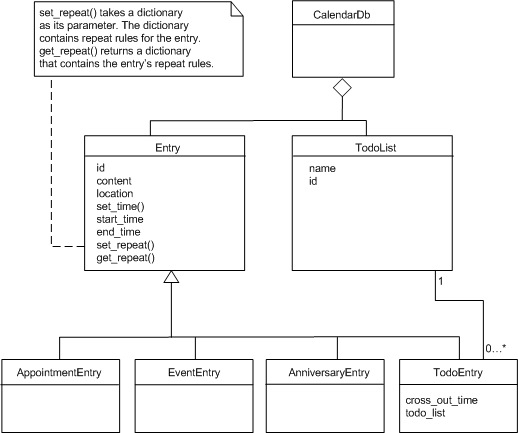
\includegraphics[width=10cm]{libcalendar-1}
\caption{The \module{calendar} module objects}
\label{libcalendar-1}
\end{figure}

Figure \ref{libcalendar-1} demonstrates the relationships of the 
\code{calendar} module objects. 

\subsection{Module Level Functions}
\label{subsec:calendarmodule}
The following free functions - functions that do not belong to any class 
- are defined in the \code{calendar} module:

\begin{funcdesc}{open}{\optional{filename=None, mode=None}}

Opens a calendar database and returns a new \class{CalendarDb} object.

If filename is \code{None}, the default database is opened.

If \var{filename} is given, it should be a full, absolute path name in
Unicode that specifies the calendar database to open. 

\var{mode} can be:

\begin{itemize}
\item \code{None}: Opens an existing calendar database.
\item \code{'c'}: Opens an existing calendar database, or creates it if it doesn't exist.
\item \code{'n'}: Creates a new, empty calendar database. If \var{filename} exists, the previous contents are erased.
\end{itemize}

\end{funcdesc}

\subsection{CalendarDb Objects}
\label{subsec:calendardb}

Calendar entries and todo lists are stored in a calendar database. There is 
one default calendar database but more calendar databases can be created by 
invoking \code{open} with parameters \code{'n' }or \code{'c'}. 

\begin{classdesc*}{CalendarDb}
\class{CalendarDb} objects have the following methods:

\begin{methoddesc}[CalendarDb]{add_appointment}{}

Creates and returns a new appointment entry \class{AppointmentEntry}. The 
entry is not added and saved into the database until \code{Entry.commit} is 
called.

\end{methoddesc}

\begin{methoddesc}[CalendarDb]{add_event}{}

Creates and returns a new event entry \class{EventEntry}. The entry is not added 
and saved into the database until \code{Entry.commit} is called.

\end{methoddesc}

\begin{methoddesc}[CalendarDb]{add_anniversary}{}

Creates and returns a new anniversary entry \class{AnniversaryEntry}. The entry 
is not added and saved into the database until \code{Entry.commit} is called.

\end{methoddesc}

\begin{methoddesc}[CalendarDb]{add_todo}{}

Creates and returns new todo entry \class{TodoEntry}. The entry is not added and 
saved into the database until \code{Entry.commit} is called.

\end{methoddesc}

\begin{methoddesc}[CalendarDb]{find_instances}{start_date, end_date, search_str=u''\optional{ ,appointments=0,events=0,anniversaries=0,todos=0}}

The parameters for this function include the start date, end date, search 
string, and optional parameters. The optional parameters define the entry 
types to be included into the search. By default all entry types are 
included. Returns a list that contains \class{Entry} instances found in the 
search. An instance is a dictionary that contains the entry ID and the 
datetime value. An entry may have several instances if it is repeated, for 
example once every week, etc. However, all the returned instances occur on 
the same day, i.e. on the first day between the start and end datetime 
values that contains instances. To search all instances between the initial 
start and end datetime values, you may have to execute several searches and 
change the start datetime value for each search. A match is detected if the 
search string is a substring of an entry's content. 

\end{methoddesc}

\begin{methoddesc}[CalendarDb]{monthly_instances}{month, appointments=0, events=0, anniversaries=0, todos=0}

The parameters for this function include \var{month} (float) and 
optional parameters. The optional parameters define the entry types to be 
returned. Returns a list that contains entry instances occurring during the 
specified calendar month.

\end{methoddesc}

\begin{methoddesc}[CalendarDb]{daily_instances}{day, appointments=0, events=0, anniversaries=0, todos=0}

The parameters for this function include \var{day} (float) and 
optional parameters. The optional parameters define the entry types to be 
returned. Returns a list that contains entry instances occurring on the 
specified day.

\end{methoddesc}

\begin{methoddesc}[CalendarDb]{add_todo_list}{\optional{name=None}}

Creates a new todo list. \var{name} sets the name of the todo list 
(Unicode). Returns the ID of the created todo list.

\end{methoddesc}

\begin{methoddesc}[CalendarDb]{export_vcalendars}{(int,...)}

Returns a \code{vcalendar} string that contains the specified entries in 
vCalendar format. The parameter for this function is a tuple that contains 
the entry IDs of the exported entries.

\end{methoddesc}

\begin{methoddesc}[CalendarDb]{import_vcalendars}{string}

Imports \code{vcalendar} entries, given in the string parameter, to the 
database. Returns a tuple that contains the unique IDs of the imported 
entries.

\end{methoddesc}

\begin{memberdesc}[CalendarDb]{todo_lists}

Contains a dictionary-like \code{TodoListDict} object for accessing
the todo lists of this database.

\end{memberdesc}

\begin{methoddesc}[CalendarDb]{__delitem__}{id}

Deletes the given calendar \code{Entry} from the database. \code{id} is the 
unique ID of the calendar \code{Entry}.

\end{methoddesc}

\begin{methoddesc}[CalendarDb]{__getitem__}{id}

Returns a calendar \code{Entry} object indicated by the unique ID. The returned 
object can be one of the following: \class{AppointmentEntry}, 
\class{EventEntry}, \class{AnniversaryEntry}, or \class{TodoEntry}. \code{id} is 
the unique ID of the calendar \code{Entry}. 

\end{methoddesc}

\begin{methoddesc}[CalendarDb]{compact}{}

Compacts the database file. The returned value (integer) indicates the 
success of compaction; a value other than zero means that the compaction was 
successful.

\end{methoddesc}

\end{classdesc*}

\subsection{Entry Objects}
\label{subsec:entry}

An \class{Entry} object represents a live view into the state of a single 
entry in the database. You can access the entries with an entry's unique ID. 
If you create a new entry using \code{db.add_appointment} etc., it is 
saved into the database only if you call the entry's \code{commit} method. 
In case an entry is already saved into the database, the autocommit mode is 
on by default and all the changes are automatically saved into the database, 
unless you call the entry's \code{begin} method. If you call the entry's 
\code{begin} method, the changes are not saved into the database until you 
call the entry's \code{commit} method. 

Database entries cannot be locked. In other words, other applications are 
able to make changes to the database entries you are using (not directly to 
the \class{EntryObjects} you are using, but to their representation in the 
database) at the same time you are modifying them, even if you use 
\code{begin} and \code{commit} methods. 

\begin{classdesc*}{Entry}
\class{Entry} objects have the following methods and properties:

\begin{memberdesc}[Entry]{content}

Sets or returns the entry's content text (Unicode).

\end{memberdesc}

\begin{methoddesc}[Entry]{commit}{}

Saves the entry or in case of a new entry adds the entry into the database. 
Note that this can be called only in case of a new entry, created with 
\code{db.add_appointment} etc., or after \code{begin} is called. 

\end{methoddesc}

\begin{methoddesc}[Entry]{rollback}{}

Undoes the changes made after last \code{commit}.

\end{methoddesc}

\begin{methoddesc}[Entry]{set_repeat}{dictionary}

Sets the repeat data of the entry. \var{dictionary} is a repeat data dictionary 
that contains all the repeat rules. For more information on repeat rules, see 
Section \ref{subsec:repeat}, Repeat Rules.

\end{methoddesc}

\begin{methoddesc}[Entry]{get_repeat}{}

Returns the repeat data dictionary of the entry.

\end{methoddesc}

\begin{memberdesc}[Entry]{location}

Sets or returns the entry's location data (Unicode), for example meeting 
room information. 

\end{memberdesc}

\begin{methoddesc}[Entry]{set_time}{start\optional{, end}}

Sets the start and end datetime values of the entry (floats). If only one 
parameter is given, the other will have the same value. 

In case of events, anniversaries, and todo entries the datetime values are 
truncated to corresponding date values.

\class{TodoEntries} can be made undated with 
\code{TodoEntry.set_time(None)}. Making the todo entry undated means 
removing the start and end date and all the repeat rules.

\end{methoddesc}

\begin{memberdesc}[Entry]{start_time}

The start datetime value (float) of the entry or \code{None} if 
the start datetime of the entry is not set.

\end{memberdesc}

\begin{memberdesc}[Entry]{end_time}

The end datetime value (float) of the entry or \code{None} if the 
end datetime of the entry is not set.

\end{memberdesc}

\begin{memberdesc}[Entry]{id}

The unique ID of the entry.

\end{memberdesc}

\begin{memberdesc}[Entry]{last_modified}

The datetime value (float) of the entry's last modification in 
universal time.

\end{memberdesc}

\begin{memberdesc}[Entry]{alarm}

The alarm datetime value (float) for the entry. \code{None} if \code{alarm} is 
not set. Alternatively removes the alarm if the value is set to \code{None}. 

Alarms can be set to all \class{Entry} types. However, only alarms set to 
Appointments and Anniversaries will actually cause an alarm; this is similar 
to the Calendar application in your Nokia device, which allows you to set an 
alarm only for Meetings and Anniversaries. In addition, alarms set to any 
entries residing in a database other than the default database do not cause 
actual alarms either.

\end{memberdesc}

\begin{memberdesc}[Entry]{priority}

The priority of the entry, which can be an integer ranging from 0 to 255. Native 
Phonebook and Calendar applications in Nokia devices use value 1 for high 
priority, 2 for normal priority, and 3 for low priority. 

\end{memberdesc}

\begin{memberdesc}[Entry]{crossed_out}

The crossed out value of an entry. A value that is interpreted as false means 
that the entry is not crossed out, whereas a value that is interpreted as true 
means that the entry is crossed out. Note that \class{TodoEntries} must also 
have a cross-out time while the other entry types cannot have one. If 
\class{TodoEntry} is crossed out using this method, the moment of crossing out 
is set to the cross-out time of the \class{TodoEntry}. See also Section 
\ref{subsubsec:todoentry}, TodoEntry, \code{cross_out_time}.

\end{memberdesc}

\begin{memberdesc}[Entry]{replication}

Sets or returns the entry's replication status, which can be one of the 
following: \code{'open'}, \code{'private',} or \code{'restricted'}.

\end{memberdesc}

\begin{methoddesc}[Entry]{as_vcalendar}{}

Returns this entry as a vCalendar string.

\end{methoddesc}

\end{classdesc*}

\subsubsection{AppointmentEntry Objects}
\label{subsubsec:appointmententry}

\begin{classdesc*}{AppointmentEntry}
\end{classdesc*}

\class{AppointmentEntry} class contains no additional methods compared to 
the \class{Entry} class from which it is derived.

\subsubsection{EventEntry}
\label{subsubsec:evententry}

\begin{classdesc*}{EventEntry}
\end{classdesc*}

\class{EventEntry} class contains no additional methods compared to the 
\class{Entry} class from which it is derived.

\subsubsection{AnniversaryEntry}
\label{subsubsec:anniversaryentry}

\begin{classdesc*}{AnniversaryEntry}
\end{classdesc*}

\class{AnniversaryEntry} class contains no additional methods compared to 
the \class{Entry} class from which it is derived.

\subsubsection{TodoEntry}
\label{subsubsec:todoentry}

\class{TodoEntry}objects represent todo entry types. They have additional 
properties compared to the \class{Entry} class from which they are derived.

\begin{classdesc*}{TodoEntry}
\class{TodoEntry}objects have the following additional properties:

\begin{memberdesc}[TodoEntry]{cross_out_time}

The cross-out date value of the entry. The value can be \code{None} meaning that 
the entry is not crossed out, or the cross-out date (float). The set value must 
be date (float). Setting a cross-out time also crosses out the entry. See also 
Section \ref{subsec:entry}, Entry Object, \code{crossed_out}.

\end{memberdesc}

\begin{memberdesc}[TodoEntry]{todo_list}

The ID of the todo list to which this entry belongs.

\end{memberdesc}

\end{classdesc*}

\subsubsection{TodoListDict}
\label{subsubsec:todolistdict}

\class{TodoListDict} objects are dictionary-like objects that enable 
accessing todo lists. 

\begin{classdesc*}{TodoListDict}
\class{TodoListDict} objects have the following property:

\begin{memberdesc}[TodoListDict]{default_list}

The ID of the default todo list.

\end{memberdesc}

\end{classdesc*}

\subsubsection{TodoList}
\label{subsubsec:todolist}

\class{TodoList} objects are dictionary-like objects that enable 
accessesing todo lists. 

\begin{classdesc*}{TodoList}
\code{TodoList} objects have the following properties:

\begin{memberdesc}[TodoList]{name}

The name of the todo list as a Unicode string.

\end{memberdesc}

\begin{memberdesc}[TodoList]{id}

Returns the ID of the todo list as an integer.

\end{memberdesc}

\end{classdesc*}

\subsection{Repeat Rules}
\label{subsec:repeat}

Repeat rules specify an entry's repeat status, that is, the recurrence of 
the entry. There are six repeat types: 

\begin{itemize}
\item \code{daily}: repeated daily
\item \code{weekly}: repeat on the specified days of the week, such as Monday and Wednesday, etc.
\item \code{monthly_by_dates}: repeat monthly on the specified dates, such as the 15th and 17th day of the month
\item \code{monthly_by_days}: repeat monthly on the specified days, such as the fourth Wednesday of the month, or the last Monday of the month
\item \code{yearly_by_date}: repeat yearly on the specified date, such as December 24
\item \code{yearly_by_day}: repeat yearly on the specified day, such as every third Tuesday of May
\end{itemize}

There are exceptions to repeat rules. For example, you can specify the 
datetime value (float) in such a way that the entry is not repeated on a 
specific day even if the repeat rule would specify otherwise.

You must set the start and end dates (floats) of the repeat. The end date 
can also be set to \code{None} to indicate that the repeating continues 
forever. You can set \code{interval} defining how often the repeat occurs, 
for example in a daily repeat: \code{1} means every day, \code{2} means 
every second day, etc. You can also set the \code{days} specifier which 
lets you explicitly specify the repeat days; for example in a weekly repeat 
you can set \code{"days":[0,2]} which sets the repeat to occur on Mondays 
and Wednesdays. If you do not set the \code{days} specifier, the repeat 
days are calculated automatically based on the start date.

You can modify repeat data by calling \code{rep_data = 
entry.get_repeat()}, then making changes to \code{rep_data} 
dictionary, and then calling \code{entry.set_repeat(rep_data)}.

Repeating can be cancelled by calling \code{entry.set_repeat} with a 
parameter that is interpreted to be false, such as 
\code{entry.set_repeat(None)}.

Repeat definition examples:

\begin{verbatim}

repeat = {"type":"daily", #repeat type
          "exceptions":[exception_day, exception_day+2*24*60*60],  
          #no appointment on those days
          "start":appt_start_date, #start of the repeat
          "end":appt_start_date+30*24*60*60, #end of the repeat
          "interval":1} #interval (1=every day, 2=every second day etc.)

repeat = {"type":"weekly", #repeat type
          "days":[0,1], #which days in a week (Monday, Tuesday)
          "exceptions":[exception_day], #no appointment on that day
          "start":appt_start_date, #start of the repeat
          "end":appt_start_date+30*24*60*60, #end of the repeat
          "interval":1}  
          #interval (1=every week, 2=every second week etc.) 

repeat = {"type":"monthly_by_days", #repeat type
          # appointments on second Tuesday and last Monday of the month
          "days":[{"week":1, "day":1},{"week":4, "day":0}],
          "exceptions":[exception_day], #no appointment on that day 
          "start":appt_start_date, #start of the repeat
          "end":appt_start_date+30*24*60*60, #end of the repeat
          "interval":1}  
          #interval (1=every month, 2=every second month etc.)

repeat = {"type":"monthly_by_dates", #repeat type
          "days":[0,15],  
          # appointments on the 1st and 16th day of the month.
          "exceptions":[exception_day], #no appointment on that day
          "start":appt_start_date, #start of the repeat
          "end":appt_start_date+30*24*60*60, #end of the repeat
          "interval":1}  
          #interval (1=every month, 2=every second month etc.)

repeat = {"type":"yearly_by_date", #repeat type
          "exceptions":[exception_day], #no appointment on that day 
          "start":appt_start_date, #start of the repeat
          "end":appt_start_date+3*365*24*60*60, #end of the repeat
          "interval":1}  
          #interval (1=every year, 2=every second year etc.)

repeat = {"type":"yearly_by_day", #repeat type
          # appointments on the second Tuesday of February
          "days":{"day":1, "week":1, "month":1},
          "exceptions":[exception_day], #no appointment on that day 
          "start":appt_start_date, #start of the repeat
          "end":appt_start_date+3*365*24*60*60, #end of the repeat
          "interval":1}  
          #interval (1=every year, 2=every second year etc.)

\end{verbatim}

% Copyright (c) 2006 Nokia Corporation
%
% Licensed under the Apache License, Version 2.0 (the "License");
% you may not use this file except in compliance with the License.
% You may obtain a copy of the License at
%
%     http://www.apache.org/licenses/LICENSE-2.0
%
% Unless required by applicable law or agreed to in writing, software
% distributed under the License is distributed on an "AS IS" BASIS,
% WITHOUT WARRANTIES OR CONDITIONS OF ANY KIND, either express or implied.
% See the License for the specific language governing permissions and
% limitations under the License.

\section{\module{calendar for EKA2} ---
  Access to calendar related services}
\label{sec:calendareka2}

\declaremodule{extension}{calendar}
\platform{S60}
\modulesynopsis{A calendar related services package.}

The \module{calendar} module offers an API to calendar services. The 
\module{calendar} module represents a Symbian agenda database as a 
dictionary-like \class{CalendarDb} object, which contains \class{Entry}
objects and which is indexed using the unique IDs of those objects. There 
are five types of entry objects: \class{AppointmentEntry}, 
\class{EventEntry}, \class{AnniversaryEntry}, \class{ReminderEntry},
 and \class{TodoEntry}. 

\class{CalendarDb} objects represent a live view into the database. If an 
entry is changed outside your Python application, the changes are visible 
immediately, and conversely any changes you commit into the database are 
visible immediately to other applications. 

All time parameters use Unix time unless stated otherwise. For more 
information on Unix time, see Section \ref{subsec:datetime}, 
Date and Time.

\subsection{Module Level Functions}
\label{subsec:calendarmodule}
The following free functions - functions that do not belong to any class 
- are defined in the \code{calendar} module:

\begin{funcdesc}{open}{\optional{filename=None, mode=None}}

Opens a calendar database and returns a new \class{CalendarDb} object.

If filename is \code{None}, the default database is opened.

If \var{filename} is given, it should contain drive letter, colon and file's name, 
but no absolute path.

\var{mode} can be:

\begin{itemize}
\item \code{None}: Opens an existing calendar database.
\item \code{'c'}: Opens an existing calendar database, or creates it if it doesn't exist.
\item \code{'n'}: Creates a new, empty calendar database. If \var{filename} exists, the previous contents are erased.
\end{itemize}

\end{funcdesc}

\subsection{CalendarDb Objects}
\label{subsec:calendardb}

Calendar entries are stored in a calendar database. There is 
one default calendar database but more calendar databases can be created by 
invoking \code{open} with parameters \code{'n' }or \code{'c'}. 

\begin{classdesc*}{CalendarDb}
\class{CalendarDb} objects have the following methods:

\begin{methoddesc}[CalendarDb]{add_appointment}{}

Creates and returns a new appointment entry \class{AppointmentEntry}. The 
entry is not added and saved into the database until \code{Entry.commit} is 
called.

\end{methoddesc}

\begin{methoddesc}[CalendarDb]{add_event}{}

Creates and returns a new event entry \class{EventEntry}. The entry is not added 
and saved into the database until \code{Entry.commit} is called.

\end{methoddesc}

\begin{methoddesc}[CalendarDb]{add_anniversary}{}

Creates and returns a new anniversary entry \class{AnniversaryEntry}. The entry 
is not added and saved into the database until \code{Entry.commit} is called.

\end{methoddesc}

\begin{methoddesc}[CalendarDb]{add_todo}{}

Creates and returns new todo entry \class{TodoEntry}. The entry is not added and 
saved into the database until \code{Entry.commit} is called.

\end{methoddesc}

\begin{methoddesc}[CalendarDb]{add_reminder}{}

Creates and returns new reminder entry \class{ReminderEntry}. The entry is not added and 
saved into the database until \code{Entry.commit} is called.

\end{methoddesc}

\begin{methoddesc}[CalendarDb]{find_instances}{start_date, end_date, search_str=u''\optional{ ,appointments=0,events=0,anniversaries=0,todos=0,reminders=0}}

The parameters for this function include the start date, end date, search 
string, and optional parameters. The optional parameters define the entry 
types to be included into the search. By default all entry types are 
included. Returns a list that contains \class{Entry} instances found in the 
search. An instance is a dictionary that contains the entry ID and the 
datetime value. An entry may have several instances if it is repeated, for 
example once every week, etc. 

\end{methoddesc}

\begin{methoddesc}[CalendarDb]{monthly_instances}{month, appointments=0, events=0, anniversaries=0, todos=0, reminders=0}

The parameters for this function include \var{month} (float) and 
optional parameters. The optional parameters define the entry types to be 
returned. Returns a list that contains entry instances occurring during the 
specified calendar month.

\end{methoddesc}

\begin{methoddesc}[CalendarDb]{daily_instances}{day, appointments=0, events=0, anniversaries=0, todos=0}

The parameters for this function include \var{day} (float) and 
optional parameters. The optional parameters define the entry types to be 
returned. Returns a list that contains entry instances occurring on the 
specified day.

\end{methoddesc}

\begin{methoddesc}[CalendarDb]{export_vcalendars}{(int,...)}

Returns a \code{vcalendar} string that contains the specified entries in 
vCalendar format. The parameter for this function is a tuple that contains 
the entry IDs of the exported entries.

\end{methoddesc}

\begin{methoddesc}[CalendarDb]{import_vcalendars}{string}

Imports \code{vcalendar} entries, given in the string parameter, to the 
database. Returns a list that contains the unique IDs of the imported 
entries.

\end{methoddesc}

\begin{methoddesc}[CalendarDb]{__delitem__}{id}

Deletes the given calendar \code{Entry} from the database. \code{id} is the 
unique ID of the calendar \code{Entry}.

\end{methoddesc}

\begin{methoddesc}[CalendarDb]{__getitem__}{id}

Returns a calendar \code{Entry} object indicated by the unique ID. The returned 
object can be one of the following: \class{AppointmentEntry}, 
\class{EventEntry}, \class{AnniversaryEntry}, \class{ReminderEntry}, 
or \class{TodoEntry}. \code{id} is the unique ID of the calendar \code{Entry}. 

\end{methoddesc}

\end{classdesc*}

\subsection{Entry Objects}
\label{subsec:entry}

An \class{Entry} object represents a live view into the state of a single 
entry in the database. You can access the entries with an entry's unique ID. 
If you create a new entry using \code{db.add_appointment} etc., it is 
saved into the database only if you call the entry's \code{commit} method. 
In case an entry is already saved into the database, the autocommit mode is 
on by default and all the changes are automatically saved into the database, 
unless you call the entry's \code{begin} method. If you call the entry's 
\code{begin} method, the changes are not saved into the database until you 
call the entry's \code{commit} method. 

Database entries cannot be locked. In other words, other applications are 
able to make changes to the database entries you are using (not directly to 
the \class{EntryObjects} you are using, but to their representation in the 
database) at the same time you are modifying them, even if you use 
\code{begin} and \code{commit} methods. 

\begin{classdesc*}{Entry}
\class{Entry} objects have the following methods and properties:

\begin{memberdesc}[Entry]{content}

Sets or returns the entry's content text (Unicode).

\end{memberdesc}

\begin{methoddesc}[Entry]{commit}{}

Saves the entry or in case of a new entry adds the entry into the database. 
Note that this can be called only in case of a new entry, created with 
\code{db.add_appointment} etc., or after \code{begin} is called. 

\end{methoddesc}

\begin{methoddesc}[Entry]{rollback}{}

Undoes the changes made after last \code{commit}.

\end{methoddesc}

\begin{methoddesc}[Entry]{set_repeat}{dictionary}

Sets the repeat data of the entry. \var{dictionary} is a repeat data dictionary 
that contains all the repeat rules. For more information on repeat rules, see 
Section \ref{subsec:repeat}, Repeat Rules.

\end{methoddesc}

\begin{methoddesc}[Entry]{get_repeat}{}

Returns the repeat data dictionary of the entry.

\end{methoddesc}

\begin{memberdesc}[Entry]{location}

Sets or returns the entry's location data (Unicode), for example meeting 
room information. 

\end{memberdesc}

\begin{methoddesc}[Entry]{set_time}{start\optional{, end}}

Sets the start and end datetime values of the entry (floats). If only one 
parameter is given, the other will have the same value. 

In case of events, anniversaries, and todo entries the datetime values are 
truncated to corresponding date values.

\class{TodoEntries} can be made undated with 
\code{TodoEntry.set_time(None)}. Making the todo entry undated means 
removing the start and end date and all the repeat rules.

\end{methoddesc}

\begin{memberdesc}[Entry]{start_time}

The start datetime value (float) of the entry or \code{None} if 
the start datetime of the entry is not set.

\end{memberdesc}

\begin{memberdesc}[Entry]{end_time}

The end datetime value (float) of the entry or \code{None} if the 
end datetime of the entry is not set.

\end{memberdesc}

\begin{memberdesc}[Entry]{id}

The unique ID of the entry.

\end{memberdesc}

\begin{memberdesc}[Entry]{last_modified}

The datetime value (float) of the entry's last modification in 
universal time.

\end{memberdesc}

\begin{memberdesc}[Entry]{originating}

An integer value indicating if the entry is an originating entry
or a modifying entry.

\end{memberdesc}

\begin{memberdesc}[Entry]{alarm}

The alarm datetime value (float) for the entry. \code{None} if \code{alarm} is 
not set. Alternatively removes the alarm if the value is set to \code{None}. 

Alarms can be set to all \class{Entry} types. However, only alarms set to 
Appointments and Anniversaries will actually cause an alarm; this is similar 
to the Calendar application in your Nokia device, which allows you to set an 
alarm only for Meetings and Anniversaries. In addition, alarms set to any 
entries residing in a database other than the default database do not cause 
actual alarms either.

\end{memberdesc}

\begin{memberdesc}[Entry]{priority}

The priority of the entry, which can be an integer ranging from 0 to 255. Native 
Phonebook and Calendar applications in Nokia devices use value 1 for high 
priority, 2 for normal priority, and 3 for low priority. 

\end{memberdesc}

\begin{memberdesc}[Entry]{crossed_out}

The crossed out value of an entry. Only valid for todo entries.
A value that is interpreted as false means 
that the entry is not crossed out, whereas a value that is interpreted as true 
means that the entry is crossed out. Note that \class{TodoEntries} must also 
have a cross-out time. If \class{TodoEntry} is crossed out using this method, 
the moment of crossing out is set to the cross-out time of the \class{TodoEntry}. 
See also Section \ref{subsubsec:todoentry}, TodoEntry, \code{cross_out_time}.

\end{memberdesc}

\begin{memberdesc}[Entry]{replication}

Sets or returns the entry's replication status, which can be one of the 
following: \code{'open'}, \code{'private',} or \code{'restricted'}.

\end{memberdesc}

\begin{methoddesc}[Entry]{as_vcalendar}{}

Returns this entry as a vCalendar string.

\end{methoddesc}

\end{classdesc*}

\subsubsection{AppointmentEntry Objects}
\label{subsubsec:appointmententry}

\begin{classdesc*}{AppointmentEntry}
\end{classdesc*}

\class{AppointmentEntry} class contains no additional methods compared to 
the \class{Entry} class from which it is derived.

\subsubsection{EventEntry}
\label{subsubsec:evententry}

\begin{classdesc*}{EventEntry}
\end{classdesc*}

\class{EventEntry} class contains no additional methods compared to the 
\class{Entry} class from which it is derived.

\subsubsection{AnniversaryEntry}
\label{subsubsec:anniversaryentry}

\begin{classdesc*}{AnniversaryEntry}
\end{classdesc*}

\class{AnniversaryEntry} class contains no additional methods compared to 
the \class{Entry} class from which it is derived.

\subsubsection{ReminderEntry}
\label{subsubsec:reminderentry}

\begin{classdesc*}{ReminderEntry}
\end{classdesc*}

\class{ReminderEntry} class contains no additional methods compared to 
the \class{Entry} class from which it is derived.

\subsubsection{TodoEntry}
\label{subsubsec:todoentry}

\class{TodoEntry}objects represent todo entry types. They have additional 
properties compared to the \class{Entry} class from which they are derived.

\begin{classdesc*}{TodoEntry}
\class{TodoEntry}objects have the following additional properties:

\begin{memberdesc}[TodoEntry]{cross_out_time}

The cross-out date value of the entry. The value can be \code{None} meaning that 
the entry is not crossed out, or the cross-out date (float). The set value must 
be date (float). Setting a cross-out time also crosses out the entry. See also 
Section \ref{subsec:entry}, Entry Object, \code{crossed_out}.

\end{memberdesc}

\end{classdesc*}


\subsection{Repeat Rules}
\label{subsec:repeat}

Repeat rules specify an entry's repeat status, that is, the recurrence of 
the entry. There are six repeat types: 

\begin{itemize}
\item \code{daily}: repeated daily
\item \code{weekly}: repeat on the specified days of the week, such as Monday and Wednesday, etc.
\item \code{monthly_by_dates}: repeat monthly on the specified dates, such as the 15th and 17th day of the month
\item \code{monthly_by_days}: repeat monthly on the specified days, such as the fourth Wednesday of the month, or the last Monday of the month
\item \code{yearly_by_date}: repeat yearly on the specified date, such as December 24
\item \code{yearly_by_day}: repeat yearly on the specified day, such as every third Tuesday of May
\end{itemize}

There are exceptions to repeat rules. For example, you can specify the 
datetime value (float) in such a way that the entry is not repeated on a 
specific day even if the repeat rule would specify otherwise.

You must set the start and end dates (floats) of the repeat. The end date 
can also be set to \code{None} to indicate that the repeating continues 
forever. You can set \code{interval} defining how often the repeat occurs, 
for example in a daily repeat: \code{1} means every day, \code{2} means 
every second day, etc. You can also set the \code{days} specifier which 
lets you explicitly specify the repeat days; for example in a weekly repeat 
you can set \code{"days":[0,2]} which sets the repeat to occur on Mondays 
and Wednesdays. If you do not set the \code{days} specifier, the repeat 
days are calculated automatically based on the start date.

You can modify repeat data by calling \code{rep_data = 
entry.get_repeat()}, then making changes to \code{rep_data} 
dictionary, and then calling \code{entry.set_repeat(rep_data)}.

Repeating can be cancelled by calling \code{entry.set_repeat} with a 
parameter that is interpreted to be false, such as 
\code{entry.set_repeat(None)}.

Repeat definition examples:

\begin{verbatim}

repeat = {"type":"daily", #repeat type
          "exceptions":[exception_day, exception_day+2*24*60*60],  
          #no appointment on those days
          "start":appt_start_date, #start of the repeat
          "end":appt_start_date+30*24*60*60, #end of the repeat
          "interval":1} #interval (1=every day, 2=every second day etc.)

repeat = {"type":"weekly", #repeat type
          "days":[0,1], #which days in a week (Monday, Tuesday)
          "exceptions":[exception_day], #no appointment on that day
          "start":appt_start_date, #start of the repeat
          "end":appt_start_date+30*24*60*60, #end of the repeat
          "interval":1}  
          #interval (1=every week, 2=every second week etc.) 

repeat = {"type":"monthly_by_days", #repeat type
          # appointments on second Tuesday and last Monday of the month
          "days":[{"week":1, "day":1},{"week":4, "day":0}],
          "exceptions":[exception_day], #no appointment on that day 
          "start":appt_start_date, #start of the repeat
          "end":appt_start_date+30*24*60*60, #end of the repeat
          "interval":1}  
          #interval (1=every month, 2=every second month etc.)

repeat = {"type":"monthly_by_dates", #repeat type
          "days":[0,15],  
          # appointments on the 1st and 16th day of the month.
          "exceptions":[exception_day], #no appointment on that day
          "start":appt_start_date, #start of the repeat
          "end":appt_start_date+30*24*60*60, #end of the repeat
          "interval":1}  
          #interval (1=every month, 2=every second month etc.)

repeat = {"type":"yearly_by_date", #repeat type
          "exceptions":[exception_day], #no appointment on that day 
          "start":appt_start_date, #start of the repeat
          "end":appt_start_date+3*365*24*60*60, #end of the repeat
          "interval":1}  
          #interval (1=every year, 2=every second year etc.)

repeat = {"type":"yearly_by_day", #repeat type
          # appointments on the second Tuesday of February
          "days":{"day":1, "week":1, "month":1},
          "exceptions":[exception_day], #no appointment on that day 
          "start":appt_start_date, #start of the repeat
          "end":appt_start_date+3*365*24*60*60, #end of the repeat
          "interval":1}  
          #interval (1=every year, 2=every second year etc.)

\end{verbatim}

% Copyright (c) 2005 Nokia Corporation
%
% Licensed under the Apache License, Version 2.0 (the "License");
% you may not use this file except in compliance with the License.
% You may obtain a copy of the License at
%
%     http://www.apache.org/licenses/LICENSE-2.0
%
% Unless required by applicable law or agreed to in writing, software
% distributed under the License is distributed on an "AS IS" BASIS,
% WITHOUT WARRANTIES OR CONDITIONS OF ANY KIND, either express or implied.
% See the License for the specific language governing permissions and
% limitations under the License.

\section{\module{e32db} ---
  Interface to the Symbian native DB}
\label{sec:e32db}

\declaremodule{extension}{e32db}
\platform{S60}
\modulesynopsis{Interface to the Symbian native DB}

\label{sec:mylabel3}
The \module{e32db} module provides an API for relational database 
manipulation with a restricted SQL syntax. For details of DBMS support, see 
the S60 SDK documentation. For examples on using this module, see \cite{PyS60Prog}.

The \module{e32db} module defines the following functions:

\begin{funcdesc}{format_rawtime}{timevalue}
Formats \var{timevalue} (Symbian time) according to the current 
system's date/time formatting rules and returns it as a Unicode string.
\end{funcdesc}

\begin{funcdesc}{format_time}{timevalue}
Formats \var{timevalue} according to the current system's date/time 
formatting rules and returns it as a Unicode string.
\end{funcdesc}

\subsection{Dbms Objects}
\label{subsec:mylabel13}

\begin{classdesc}{Dbms}{}
Creates a Dbms object. Dbms objects support basic 
operations on a database. 
\end{classdesc}

Dbms objects have the following methods:

\begin{methoddesc}[Dbms]{begin}{}
Begins a transaction on the database.
\end{methoddesc}

\begin{methoddesc}[Dbms]{close}{}
Closes the database object. It is safe to try to close a database object 
even if it is not open.
\end{methoddesc}

\begin{methoddesc}[Dbms]{commit}{}
Commits the current transaction.
\end{methoddesc}

\begin{methoddesc}[Dbms]{compact}{}
Compacts the database, reclaiming unused space in the database file. 
\end{methoddesc}

\begin{methoddesc}[Dbms]{create}{dbname}
Creates a database with path \var{dbname}.
\end{methoddesc}

\begin{methoddesc}[Dbms]{execute}{query}
Executes an SQL \var{query}. On success, returns \code{0} if a DDL
(SQL schema update) statement was executed. Returns the number of rows
inserted, updated, or deleted, if a DML (SQL data update) statement
was executed.
\end{methoddesc}

\begin{methoddesc}[Dbms]{open}{dbname}
Opens the database in file \var{dbname}. This should be a full 
Unicode path name, for example, \code{u'c:\e\e foo.db'}.
\end{methoddesc}

\begin{methoddesc}[Dbms]{rollback}{}
Rolls back the current transaction.
\end{methoddesc}

\subsection{DB_view Objects}
\label{subsec:mylabel14}

\begin{classdesc}{Db_view}{}
Creates a \class{Db_view} object. \class{DB_view} objects generate 
rowsets from a SQL query. They provide functions to parse and evaluate the 
rowsets.
\end{classdesc}

Db_view objects have the following methods:

\begin{methoddesc}[Db_view]{col}{column}
Returns the value in \var{column}. The first column of the rowset has the index 
\code{1}. If the type of the column is not supported, a \exception{TypeError} is 
raised. See Table \ref{tab:sqltypes} for a list of supported data types.
\end{methoddesc}

\begin{methoddesc}[Db_view]{col_count}{}
Returns the number of columns defined in the rowset.
\end{methoddesc}

\begin{methoddesc}[Db_view]{col_length}{column}
Gets the length of the value in \var{column}. Empty columns have 
a length of zero; non-empty numerical and date/time columns have a length of 
1. For text columns, the length is the character count, and for binary 
columns, the length is the byte count.
\end{methoddesc}

\begin{methoddesc}[Db_view]{col_raw}{column}
Extracts the value of \var{column} as raw binary data, and 
returns it as a Python string. The first column of the rowset has the index 
1. See Table \ref{tab:sqltypes} for a list of supported data types.
\end{methoddesc}

\begin{methoddesc}[Db_view]{col_rawtime}{column}
Extracts the value of a date/time column at index \var{column} as a
long integer, which represents the raw Symbian time value. The first
column of the rowset has the index 1.  See Table \ref{tab:sqltypes} for a list of the
supported data types.
\end{methoddesc}

\begin{methoddesc}[Db_view]{col_type}{column}
Returns the numeric type of the given column as an integer from a 
Symbian-specific list of types. This function is used in the implementation 
of method \method{col}.
\end{methoddesc}

\begin{methoddesc}[Db_view]{count_line}{}
Returns the number of rows available in the rowset.
\end{methoddesc}

\begin{methoddesc}[Db_view]{first_line}{}
Positions the cursor on the first row in the rowset.
\end{methoddesc}

\begin{methoddesc}[Db_view]{get_line}{}
Gets the current row data for access.
\end{methoddesc}

\begin{methoddesc}[Db_view]{is_col_null}{column}
Tests whether \var{column} is empty. Empty columns can be 
accessed like normal columns. Empty numerical columns return a \code{0} or 
an equivalent value, and text and binary columns have a zero length.
\end{methoddesc}

\begin{methoddesc}[Db_view]{next_line}{}
Moves the cursor to the next row in the rowset.
\end{methoddesc}

\begin{methoddesc}[Db_view]{prepare}{db, query}
Prepares the view object for evaluating an SQL select statement. 
\var{db} is a \class{Dbms} object and \var{query}
the SQL query to be executed.
\end{methoddesc}

\subsection{Mapping Between SQL and Python Data Types }
\label{subsec:mapping}
See Table \ref{tab:sqltypes} for a summary of mapping between SQL and 
Python data types. The \method{col} function can extract any value except 
\code{LONG VARBINARY} and return it as the proper Python value. In 
addition, the \method{col_raw} function can extract any column type 
except \code{LONG VARCHAR} and \code{LONG VARBINARY} as raw binary data 
and return it as a Python string.

Inserting, updating, or searching for \code{BINARY}, \code{VARBINARY}, 
or \code{LONG VARBINARY} values is not supported. \code{BINARY} and 
\code{VARBINARY} values can be read with \method{col} or 
\method{col_raw}.

\begin{table}[htbp]
\begin{center}
\begin{tabular}{|p{117pt}|p{144pt}|p{99pt}|p{63pt}|}
\hline
SQL type& 
Symbian column type (in the DBMS C++ API)& 
Python type& 
Supported \\
\hline
\textsf{BIT}& 
\textsf{EDbColBit}& 
\raisebox{-10.50ex}[0cm][0cm]{int}& 
\raisebox{-27.00ex}[0cm][0cm]{yes} \\
\cline{1-2} 
\textsf{TINYINT}& 
\textsf{EDbColInt8}& 
 & 
  \\
\cline{1-2} 
\textsf{UNSIGNED TINYINT}& 
\textsf{EDbColUint8}& 
 & 
  \\
\cline{1-2} 
\textsf{SMALLINT}& 
\textsf{EDbColInt16}& 
 & 
  \\
\cline{1-2} 
\textsf{UNSIGNED SMALLINT}& 
\textsf{EDbColUint16}& 
 & 
  \\
\cline{1-2} 
\textsf{INTEGER}& 
\textsf{EDbColInt32}& 
 & 
  \\
\cline{1-2} 
\textsf{UNSIGNED INTEGER}& 
\textsf{EDbColUint32}& 
 & 
  \\
\cline{1-2} 
\textsf{COUNTER}& 
\textsf{EDbColUint32 (}with the\textsf{ TDbCol::EAutoIncrement }attribute\textsf{)}& 
 & 
  \\
\cline{1-3} 
\textsf{BIGINT}& 
\textsf{EDbColInt64}& 
long& 
  \\
\cline{1-3} 
\textsf{REAL}& 
\textsf{EDbColReal32}& 
\raisebox{-4.50ex}[0cm][0cm]{float  \par }& 
  \\
\cline{1-2} 
\textsf{FLOAT}& 
\raisebox{-3.00ex}[0cm][0cm]{\textsf{EDbColReal64} \par \textsf{}}& 
 & 
  \\
\cline{1-1} 
\textsf{DOUBLE}& 
 & 
 & 
  \\
\cline{1-1} 
\textsf{DOUBLE PRECISION}& 
 & 
 & 
  \\
\cline{1-3} 
\textsf{DATE}& 
\raisebox{-3.00ex}[0cm][0cm]{\textsf{EDbColDateTime} \par \textsf{}}& 
\raisebox{-3.00ex}[0cm][0cm]{float \par (or long, with \textsf{col_rawtime()})}& 
  \\
\cline{1-1} 
\textsf{TIME}& 
 & 
 & 
  \\
\cline{1-1} 
\textsf{TIMESTAMP}& 
 & 
 & 
  \\
\cline{1-3} 
\textsf{CHAR(n)}& 
\raisebox{-1.50ex}[0cm][0cm]{\textsf{EDbColText}}& 
\raisebox{-3.00ex}[0cm][0cm]{Unicode}& 
  \\
\cline{1-1} 
\textsf{VARCHAR(n)}& 
 & 
 & 
  \\
\cline{1-2} 
\textsf{LONG VARCHAR}& 
\textsf{EDbColLongText}& 
 & 
  \\
\hline
\textsf{BINARY(n)}& 
\raisebox{-1.50ex}[0cm][0cm]{\textsf{EDbColBinary} \par \textsf{}}& 
\raisebox{-1.50ex}[0cm][0cm]{str}& 
\raisebox{-1.50ex}[0cm][0cm]{read only} \\
\cline{1-1} 
\textsf{VARBINARY(n)}& 
 & 
 & 
  \\
\hline
\textsf{LONG VARBINARY}& 
\textsf{EDbColLongBinary}& 
n/a& 
no \\
\hline
\end{tabular}
\caption{Mapping between SQL and Python types}
\label{tab:sqltypes}
\end{center}
\end{table}


\subsection{Date and Time Handling}
\label{subsec:mylabel15}
The functions \method{col} and \textsf{format_time} use Unix time, 
seconds since January 1, 1970, 00:00:00 UTC, as the time format. Internally 
the database uses the native Symbian time representation that provides 
greater precision and range than the Unix time. The native Symbian time 
format is a 64-bit value that represents microseconds since January 1st 0 AD 
00:00:00 local time, nominal Gregorian. BC dates are represented by negative 
values. Since converting this format to Unix time and back may cause slight 
round-off errors, you have to use the functions \function{col_rawtime} and 
\function{format_rawtime} if you need to be able to handle these values 
with full precision.

The representation of date and time literals in SQL statements depends on 
the current system date and time format. Note that the only accepted 
ordering of day, month, and year is the one that the system is currently 
configured to use. Dates in other order are rejected. The recommended way to 
form date/time literals for SQL statements is to use the functions 
\function{format_time} or \function{format_rawtime} that format the given 
date/time values properly according to the current system's date/time format 
settings.

% Copyright (c) 2005 Nokia Corporation
%
% Licensed under the Apache License, Version 2.0 (the "License");
% you may not use this file except in compliance with the License.
% You may obtain a copy of the License at
%
%     http://www.apache.org/licenses/LICENSE-2.0
%
% Unless required by applicable law or agreed to in writing, software
% distributed under the License is distributed on an "AS IS" BASIS,
% WITHOUT WARRANTIES OR CONDITIONS OF ANY KIND, either express or implied.
% See the License for the specific language governing permissions and
% limitations under the License.

\section{\module{e32dbm} ---
  DBM implemented using the Symbian native DBMS}
\label{sec:e32dbm}

\declaremodule{}{e32dbm}
\platform{S60}
\modulesynopsis{DBM implemented using the Symbian native DBMS}

The \module{e32dbm} module provides a DBM API that uses the native
Symbian RDBMS as its storage back-end. The module API resembles that
of the \refmodule{gdbm} module. The main differences are:

\begin{itemize}
\item The \method{firstkey()} - \method{nextkey()} interface for iterating through keys is not supported. Use the \code{"for key in db"} idiom or the \method{keys} or \method{keysiter} methods instead.
\item This module supports a more complete set of dictionary features than \refmodule{gdbm}
\item The values are always stored as Unicode, and thus the values returned are Unicode strings even if they were given to the DBM as normal strings.
\end{itemize}
\subsection{Module Level Functions}
\label{subsec:mylabel16}

The \module{e32dbm} defines the following functions:

\begin{funcdesc}{open}{dbname\optional{,flags, mode}}
Opens or creates the given database file and returns an \class{e32dbm}
object.  Note that \var{dbname} should be a full path name, for
example, \textsf{u'c:$\backslash
\backslash $foo.db'}. Flags can be:

\begin{itemize}
\item \code{'r'}: opens an existing database in read-only mode. This is the default value.
\item \code{'w'}: opens an existing database in read-write mode.
\item \code{'c'}: opens a database in read-write mode. Creates a new database if the database does not exist.
\item \code{'n'}: creates a new empty database and opens it in read-write mode.
\end{itemize}

If the character \code{'f'} is appended to flags, the database is opened in \textit{fast mode}. In 
fast mode, updates are written to the database only when one of these 
methods is called: \method{sync}, \method{close}, \method{reorganize}, or 
\method{clear}.
\end{funcdesc}

Since the connection object destructor calls \method{close}, it is not 
strictly necessary to close the database before exiting to ensure that data 
is saved, but it is still good practice to call the \method{close} method 
when you are done with using the database. Closing the database releases the 
lock on the file and allows the file to be reopened or deleted without 
exiting the interpreter.

If you plan to do several updates, it is highly recommended that you open 
the database in fast mode, since inserts and updates are more efficient when 
they are bundled together in a larger transaction. This is especially 
important when you plan to insert large amounts of data, since inserting 
records to \refmodule{e32db} is very slow if done one record at a time.

\subsection{e32dbm Objects}
The \module{e32dbm} objects returned by the \method{open} function support 
most of the standard dictionary methods. The supported dictionary methods 
are:

\begin{itemize}
\item \code{__getitem__}
\item \code{__setitem__}
\item \code{__delitem__}
\item \code{has_key}
\item \code{update}
\item \code{__len__}
\item \code{__iter__}
\item \code{iterkeys}
\item \code{iteritems}
\item \code{itervalues}
\item \code{get}
\item \code{setdefault}
\item \code{pop}
\item \code{popitem}
\item \code{clear}
\end{itemize}

These work the same way as the corresponding methods in a normal dictionary.

In addition, \class{e32dbm} objects have the following methods:

\begin{methoddesc}[e32dbm]{close}{}
Closes the database. In fast mode, commits all pending updates to disk. 
\method{close} raises an exception if called on a database that is not open.
\end{methoddesc}

\begin{methoddesc}[e32dbm]{reorganize}{}
Reorganizes the database. Reorganization calls \method{compact} on the 
underlying \refmodule{e32db} database file, which reclaims unused space in the 
file. Reorganizing the database is recommended after several updates.
\end{methoddesc}

\begin{methoddesc}[e32dbm]{sync}{}
In fast mode, commits all pending updates to disk.
\end{methoddesc}



\chapter{Standard Library Support and Extensions \label{s60lib}}

% Copyright (c) 2005 Nokia Corporation
%
% Licensed under the Apache License, Version 2.0 (the "License");
% you may not use this file except in compliance with the License.
% You may obtain a copy of the License at
%
%     http://www.apache.org/licenses/LICENSE-2.0
%
% Unless required by applicable law or agreed to in writing, software
% distributed under the License is distributed on an "AS IS" BASIS,
% WITHOUT WARRANTIES OR CONDITIONS OF ANY KIND, either express or implied.
% See the License for the specific language governing permissions and
% limitations under the License.

\section{Support for Python Standard Library}
\label{sec:standard}

The standard library support in Python for S60 is summarized in Table 
\ref{standardsupport}. For API descriptions, see \cite{PyLibRef}.

\begin{center}
\begin{longtable}{|l|l|l|p{200pt}|}
\hline
{\bf Name}& 
{\bf Type}& 
{\bf Status}& 
{\bf Remarks} \\
\hline
\code{{\_}testcapi}& 
PYD& 
Y& 
 \\
\hline
\code{anydbm}& 
PY& 
X& 
DBM API is implemented by PY \code{e32dbm} that relies on PYD \code{e32db} (see Chapter \ref{sec:e32dbm}, e32dbm Module) \\
\hline
\code{atexit}& 
PY& 
X& 
 \\
\hline
\code{base64}& 
PY& 
X& 
 \\
\hline
\code{bdb}& 
PY& 
(X)& 
 \\
\hline
\code{binascii}& 
built-in& 
X& 
 \\
\hline
\code{cmd}& 
PY& 
(X)& 
 \\
\hline
\code{code}& 
PY& 
X& 
 \\
\hline
\code{codecs}& 
PY& 
X& 
 \\
\hline
\code{codeop}& 
PY& 
X& 
 \\
\hline
\code{copy}& 
PY& 
X& 
 \\
\hline
\code{copy{\_}reg}& 
PY& 
X& 
 \\
\hline
\code{cStringIO}& 
built-in& 
X& 
 \\
\hline
\code{dis}& 
PY& 
(X)& 
 \\
\hline
\code{errno}& 
built-in& 
X& 
 \\
\hline
\code{exceptions}& 
built-in& 
X& 
 \\
\hline
\code{{\_}{\_}future{\_}{\_}}& 
PY& 
X& 
 \\
\hline
\code{httplib}& 
PY& 
X& 
 \\
\hline
\code{imp}& 
built-in& 
X& 
 \\
\hline
\code{keyword}& 
PY& 
X& 
 \\
\hline
\code{linecache}& 
PY& 
X& 
 \\
\hline
\code{marshal}& 
built-in& 
X& 
 \\
\hline
\code{math}& 
built-in& 
X& 
 \\
\hline
\code{md5}\footnote{Derived from the RSA Data Security, Inc. MD5 Message-Digest Algorithm.}& 
built-in& 
X& 
 \\
\hline
\code{mimetools}& 
PY& 
X& 
 \\
\hline
\code{operator}& 
built-in& 
X& 
 \\
\hline
\code{os, os.path}& 
PY& 
X& 
Wraps built-in \code{e32posix}. Limitations discussed in Section \ref{subsec:limitations}, Limitations and Areas of Development. \\
\hline
\code{pdb}& 
PY& 
(X)& 
 \\
\hline
\code{quopri}& 
PY& 
X& 
 \\
\hline
Name& 
Type& 
Status& 
Remarks \\
\hline
\code{random}& 
PY& 
X& 
 \\
\hline
\code{re}& 
PY& 
X& 
Uses PY \code{sre} as its engine. \\
\hline
\code{repr}& 
PY& 
X& 
 \\
\hline
\code{rfc822}& 
PY& 
X& 
 \\
\hline
\code{select}& 
PY& 
X& 
A minimal implementation: \code{select} is supported only for input from sockets. \\
\hline
\code{socket}& 
PY& 
X& 
Requires PYD \code{e32socket}. Contains extensions as described in Section \ref{subsec:socket}, socket Module. Limitations discussed in Section \ref{subsec:limitations}, Limitations and Areas of Development.  \\
\hline
\code{sre}& 
PY& 
X& 
Wraps built-in \code{{\_}sre}. \\
\hline
\code{string}& 
PY& 
X& 
 \\
\hline
\code{StringIO}& 
PY& 
X& 
 \\
\hline
\code{struct}& 
built-in& 
X& 
 \\
\hline
\code{sys}& 
built-in& 
X& 
 \\
\hline
\code{thread}& 
built-in& 
X& 
Contains extensions as described in Section \ref{subsec:thread}, thread Module \\
\hline
\code{threading}& 
PY& 
(X)& 
 \\
\hline
\code{time}& 
built-in& 
X& 
 \\
\hline
\code{traceback}& 
PY& 
X& 
 \\
\hline
\code{types}& 
PY& 
X& 
 \\
\hline
\code{urllib}& 
PY& 
X& 
 \\
\hline
\code{urlparse}(urlsplit only)& 
PY& 
X& 
 \\
\hline
\code{uu}& 
PY& 
X& 
 \\
\hline
\code{warnings}& 
PY& 
X& 
 \\
\hline
\code{whichdb}& 
PY& 
X& 
 \\
\hline
\code{xreadlines}& 
built-in& 
X& 
 \\
\hline
\code{zipfile}& 
PY& 
X& 
 \\
\hline
\code{zlib}& 
PYD& 
X& 
 \\
\hline
\caption{Status of library module support.}
\label{standardsupport}
\end{longtable}
\end{center}

Table \ref{standardsupport} uses the following coding for module types:

\begin{itemize}
\item PY -- module is implemented in Python.
\item Built-in -- module is a built-in C/C++ module.
\item PYD -- module is a dynamically loadable C/C++ module.
\end{itemize}
For support status, the following codes are used:

\begin{enumerate}
\item[\textbullet] X -- included to the Series 60 Python distribution.
\item[\textbullet] (X) -- not included to the Series 60 Python distribution, but works both on phone and SDK.
\item[\textbullet] Y -- included only to the SDK distribution.
\end{enumerate}

% Copyright (c) 2005 - 2007 Nokia Corporation
%
% Licensed under the Apache License, Version 2.0 (the "License");
% you may not use this file except in compliance with the License.
% You may obtain a copy of the License at
%
%     http://www.apache.org/licenses/LICENSE-2.0
%
% Unless required by applicable law or agreed to in writing, software
% distributed under the License is distributed on an "AS IS" BASIS,
% WITHOUT WARRANTIES OR CONDITIONS OF ANY KIND, either express or implied.
% See the License for the specific language governing permissions and
% limitations under the License.

\section{Extensions to Standard Library Modules}
\label{extensions}

The following standard modules have been extended.

\subsection{\module{thread} ---
  S60 extensions to standard thread module} 
\label{subsec:thread}

\declaremodule{extension}{thread}
\modulesynopsis{S60 extensions to standard thread module.}

The following function has been added to the standard \code{thread} 
module:

\begin{funcdesc}{ao_waittid}{thread_id}

Synchronizes with the end of the execution of the thread identified by the given 
\var{thread_id}. The implementation is based on a Symbian OS active object. 
For the blocking behavior, see Section \ref{subsec:Aolock}, Ao_lock Type.

\end{funcdesc}

\subsection{\module{socket} ---
  S60 extensions to standard socket module} 
\label{subsec:socket}

\declaremodule{extension}{socket}
\modulesynopsis{Extensions to standard socket module.}

Bluetooth (BT) support has been added to the standard \code{socket} 
module. The following related constants and functions are defined:

\begin{notice}[note]
In release 1.0 the functions \code{bt_advertise_service}, 
\code{bt_obex_receive}, and 
\code{bt_rfcomm_get_available_server_channel} incorrectly 
expected to be given the internal \code{e32socket.socket} object as the 
socket parameter instead of the proper \code{socket} object. Now the 
functions work correctly. The old calling convention is still supported but 
it is deprecated and may be removed in a future release.
\end{notice}

\begin{datadesc}{AF_BT}

Represents the Bluetooth address family.

\end{datadesc}

\begin{datadesc}{BTPROTO_RFCOMM}

This constant represents the Bluetooth protocol RFCOMM.

\end{datadesc}

\begin{datadesc}{RFCOMM}
\end{datadesc}
\begin{datadesc}{OBEX}

Bluetooth service classes supported by \code{bt_advertise_service}.

\end{datadesc}

\begin{datadesc}{AUTH}
\end{datadesc}
\begin{datadesc}{ENCRYPT}
\end{datadesc}
\begin{datadesc}{AUTHOR}

Bluetooth security mode flags.

\end{datadesc}

\begin{funcdesc}{bt_advertise_service}{name, socket, flag, class}

Sets a service advertising the service \var{name} (Unicode) on local channel 
that is bound to \var{socket}. If \var{flag} is \code{True}, the advertising is 
turned on, otherwise it is turned off. The service class to be advertised is 
either \code{RFCOMM} or \code{OBEX}.

\end{funcdesc}

\begin{funcdesc}{bt_discover}{\optional{address}}

Performs the Bluetooth device discovery (if the optional BT device address 
is not given) and the discovery of RFCOMM class services on the chosen 
device. Returns a pair: BT device address, dictionary of services, where 
Unicode service name is the key and the corresponding port is the value.

\end{funcdesc}

\begin{funcdesc}{bt_obex_discover}{\optional{address}}

Same as \code{discover}, but for discovery of OBEX class services on the 
chosen device.

\end{funcdesc}

\begin{funcdesc}{bt_obex_send_file}{address, channel, filename}

Sends file \var{filename} (Unicode) wrapped into an OBEX object 
to remote \var{address}, \var{channel}.

\end{funcdesc}

\begin{funcdesc}{bt_obex_receive}{socket, filename}

Receives a file as an OBEX object, unwraps and stores it into \var{filename} 
(Unicode). \var{socket} is a bound \code{OBEX} socket.

\end{funcdesc}

\begin{funcdesc}{bt_rfcomm_get_available_server_channel}{socket}

Returns an available RFCOMM server channel for \var{socket}.

\end{funcdesc}

\begin{funcdesc}{set_security}{socket, mode}

Sets the security level of the given bound \var{socket}. The 
\var{mode} is an integer flag that is formed using a binary 
\code{or} operation of one or more of: \code{AUTH} (authentication), 
\code{ENCRYPT}, \code{AUTHOR} (authorization). Example: 
\code{set_security(s, AUTH | AUTHOR)}.

\end{funcdesc}

\begin{notice}[note]
When listening to a Bluetooth socket on the phone, it is necessary to set 
the security level.
\end{notice}

\begin{notice}[note]
SSL is not supported in S60 1st Edition. SSL client certificates are 
not supported at all.
\end{notice}

For examples on the usage of these functions, see Programming with Python for 
S60 Platform \cite{PyS60Prog}.

Setting default Access Point (AP) has been added to the standard \code{socket} 
module. The following related constants and functions are defined:

\begin{funcdesc}{select_access_point}{}
This opens popup selection where access points are listed and can be selected.
Returns selected access point id.
\end{funcdesc}

\begin{funcdesc}{access_point}{apid}
This creates access point object by given apid. Returns access point object.
\end{funcdesc}

\begin{funcdesc}{set_default_access_point}{apo}
This sets the default access point that is used when socket is opened. Setting 
\var{apo} to \code{"None"} will clear default access point.
\end{funcdesc}

\begin{funcdesc}{access_points}{}
This lists access points id's and names that are available. 
\end{funcdesc}

Example 1:
\begin{verbatim}
#access point is selected from the list
apid = select_access_point()
apo = access_point(apid)
set_default_access_point(apo)

s = socket(AF_INET, SOCK_STREAM)
print apo.ip()
s.connect(('www.sourceforge.net',80))
s.send('GET /\r\n\r\n')
s.recv(100)
s.close()
apo.stop()

\end{verbatim}

Example 2:
\begin{verbatim}
#Access point id is already known
apo = access_point(1)
set_default_access_point(apo) 

s = socket(AF_INET, SOCK_STREAM)
s.connect(('www.sourceforge.net',80))
s.send('GET /\r\n\r\n')
s.recv(100)
s.close()
apo.stop()
\end{verbatim}

Example 3:
\begin{verbatim}
#display interface ip.
#access point is selected from the list
apid = select_access_point()
apo = access_point(apid)
apo.start()
#Note that ip-address is given by operator, if static ip-address is not defined,
#when connection is started
print apo.ip()
#When connection is closed dynamic ip-address is released
apo.stop()
\end{verbatim}



\chapter{Extending and Embedding \label{s60ext}}

% Copyright (c) 2005 Nokia Corporation
%
% Licensed under the Apache License, Version 2.0 (the "License");
% you may not use this file except in compliance with the License.
% You may obtain a copy of the License at
%
%     http://www.apache.org/licenses/LICENSE-2.0
%
% Unless required by applicable law or agreed to in writing, software
% distributed under the License is distributed on an "AS IS" BASIS,
% WITHOUT WARRANTIES OR CONDITIONS OF ANY KIND, either express or implied.
% See the License for the specific language governing permissions and
% limitations under the License.

\section{Python/C API Extensions}
\label{capiextensions}

The native API exported by the interpreter in S60 environment
consists of class \class{CSPyInterpreter}, Python/C API (see
\cite{PyCAPI}) and and a small set of extensions to Python/C API.

\subsection{class \class{CSPyInterpreter}}
The class \class{CSPyInterpreter} offers an interface for initializing the 
interpreter and for running scripts. It exports the following public 
interface:
\begin{verbatim}
static CSPyInterpreter* 
NewInterpreterL(TBool aCloseStdlib = ETrue,
                void(*aStdioInitFunc)(void*) = NULL,
                void* aStdioInitCookie = NULL);
TInt RunScript(int argc, char** argv);
void PrintError();
void (*iStdI)(char* buf, int n);
void (*iStdO)(const char* buf, int n);
\end{verbatim}

The caller of the constructor \cfunction{CSPyInterpreter::NewInterpreterL()} may 
provide its own function \var{aStdioInitFunc} for initializing Symbian OS 
STDLIB's standard I/O descriptors. It gets called with the argument 
\var{aStdioInitCookie}. The \ctype{CSPyInterpreter} class can also be 
requested to leave STDLIB open at its destruction.

The \method{RunScript} method establishes a Python 
interpreter context and runs the script file whose full path name is in 
\code{argv[0]} with the given argument vector. After completion, it leaves 
the interpreter context and returns a Symbian error code to indicate success 
or failure.

The \method{CSPyInterpreter::PrintError} method can be used to print current 
Python exception information to the standard error output.

\subsection{Extensions to Python/C API}

\subsubsection{Defined in symbian_python_ext_util.h}

\begin{cfuncdesc}{PyObject*}{SPyErr_SetFromSymbianOSErr}{int error}
Sets Python exception of type \textsf{PyExc_SymbianError} with the value 
field set to symbolic name of the Symbian OS enumeration value 
\textsf{error} and returns \textsf{NULL}. In case \textsf{error} has the 
special value \textsf{KErrPython}, it assumes that a Python exception has 
already been set and returns \textsf{NULL}.
\end{cfuncdesc}

The following functions can be used for storing the global data in a module 
implementation. They are thin wrappers around 
\cfunction{PyDict_SetItem},  
\cfunction{PyDict_SetItemString}, \cfunction{PyDict_GetItem}, 
\cfunction{PyDict_GetItemString}, \cfunction{PyDict_DelItem} and 
\cfunction{PyDict_DelItemString}, respectively, and can be used in the same way. 
The data is stored in a special completely global dictionary shared by all modules and threads in the current interpreter.

\begin{cfuncdesc}{int}{SPyAddGlobal}{PyObject *key, PyObject *value}\end{cfuncdesc}
\begin{cfuncdesc}{int}{SPyAddGlobalString}{char *key, PyObject *value}\end{cfuncdesc}
\begin{cfuncdesc}{PyObject*}{SPyGetGlobal}{PyObject *key}\end{cfuncdesc}
\begin{cfuncdesc}{PyObject*}{SPyGetGlobalString}{char *key}\end{cfuncdesc}
\begin{cfuncdesc}{void}{SPyRemoveGlobal}{PyObject *key}\end{cfuncdesc}
\begin{cfuncdesc}{void}{SPyRemoveGlobalString}{char *key}\end{cfuncdesc}

\subsubsection{Defined in python_globals.h}
\begin{cvardesc}{PyThreadState*}{PYTHON_TLS->thread_state}
Current thread state.
\end{cvardesc}

Thread state and interpreter lock management must be performed
according to the instructions; see \cite{PyCAPI}. Python for S60
Platform extends the Python/C API by offering a facility for querying
the related Python thread state (\code{PYTHON_TLS->thread_state}) from the context of the currently running thread. This
can be used to re-establish the interpreter context with
\cfunction{PyEval_RestoreThread} in C/C++ code.

To save/restore the interpreter context:
\begin{verbatim}
Py_BEGIN_ALLOW_THREADS
/* ...your code... */
Py_END_ALLOW_THREADS
\end{verbatim}

To restore/save the interpreter context:
\begin{verbatim}
PyEval_RestoreThread(PYTHON_TLS-$>$thread_state)
/* ...your code... */
PyEval_SaveThread()
\end{verbatim}

\subsubsection{Defined in pythread.h}

\begin{cfuncdesc}{int}{PyThread_AtExit}{void(*)()}
An extenstion to the standard \refmodule{thread} module's C API that
can be used for registering thread-specific exit functions. In the
main thread calling this function has the same effect as calling
\cfunction{Py_AtExit}. For more information, see \cite{PyLibRef}.
\end{cfuncdesc}

% Copyright (c) 2005 Nokia Corporation
%
% Licensed under the Apache License, Version 2.0 (the "License");
% you may not use this file except in compliance with the License.
% You may obtain a copy of the License at
%
%     http://www.apache.org/licenses/LICENSE-2.0
%
% Unless required by applicable law or agreed to in writing, software
% distributed under the License is distributed on an "AS IS" BASIS,
% WITHOUT WARRANTIES OR CONDITIONS OF ANY KIND, either express or implied.
% See the License for the specific language governing permissions and
% limitations under the License.

\section{Extending Python for S60}
\label{extending}
The general rules and guidelines for writing Python extensions apply
in the S60 Python environment as well; for more information, see
\cite{PyExtEmb}.  The Python/C API is available, see \cite{PyCAPI} In
addition, for an example on porting a simple extension to S60, see
\cite{PyS60Prog}.

The issues that need to be considered in the implementation of the
extension modules include:

\begin{itemize}
\item Preparation of the data structures that make the C/C++ coded extensions visible to the Python interpreter and make it possible to perform calls from Python to C/C++ code
\item Conversions between C/C++ representations of the Python objects and object types used in the extension code
\item Maintenance of the reference counts of the C/C++ representations of the Python objects
\item Passing of exceptions between C/C++ code and Python
\item Management of interpreter's thread state and the interpreter lock
\end{itemize}
In addition to the concerns common for all Python C extensions, the 
following principles should be considered when implementing new Python 
interfaces in the S60 environment:

\begin{itemize}
\item Maximize the usage of Python's built-in types at the interfaces.
\item Related to the above: design interfaces in such a way that information can be passed between them with minimal conversions.
\item Convert Symbian operating system exceptions / errors to Python exceptions.
\item Unicode strings are used at the interfaces to represent text that gets shown on the GUI. They can be passed to and from Symbian operating system without conversions.
\item While performing potentially long-lasting / blocking calls from an extension implementation to services outside the interpreter, the interpreter lock must be released and then re-acquired after the call.
\item Rather than always implementing a thin wrapper on top of a Symbian OS facility, consider the actual task for which the script writer needs the particular interface. For example, if the task involves interaction with the users using the GUI, the script writer's interest may well be limited to performing the interaction / information exchange in a way that is compatible with the UI style rather than having full control of the low-level details of the GUI implementation.
\item The C/C++ implementation of a Python interface should be optimized for performance and covering access to the necessary features of the underlying Platform. Where necessary, the Python programming interface can be further refined by wrapper modules written in Python.
\end{itemize}

An extension module is packaged in its own dynamically loadable
library that must be installed into \file{\textbackslash system\textbackslash libs} directory and named
\file{module_name.pyd}. The module initialization function
must be exported at ordinal 1. The module identification is based on
the filename only. As a special feature of PyS60, an optional module
finalizer function may be exported at ordinal 2.

The macro versions of memory-management functions \cfunction{PyMem_MALLOC} 
and \cfunction{PyObject_NEW} are not included. Use the functions 
\cfunction{PyMem_Malloc} and \cfunction{PyObject_New} instead.

\subsection{Services for Extensions}
S60 Python Platform implements an adaptation layer between S60 
UI application framework and script language UI extensions to simplify UI 
extension development. This API is used by the implementation of the 
\textsf{appuifw} module but not exported in the current release. Some 
general utility services for extensions are also provided, see 
Chapter \ref{capiextensions}.

\subsection{Example}
This extension code snippet demonstrates some of the issues mentioned in this chapter, such as:

\begin{itemize}
\item Conversion from Python data types, usage of built-in data types at extension interface, usage of Unicode strings (lines 8-12)
\item Maintenance of the reference counts (line 36)
\item Passing of exceptions between C/C++ code and Python (line 34)
\item Releasing the interpreter lock while performing a blocking call to a service outside the interpreter (lines 29, 31)
\item Simplifying the API to the note facility of the Platform
\end{itemize}

\begin{verbatim}
01 extern "C" PyObject *
02 note(PyObject* /*self*/, PyObject *args)
03 {
04   TInt error = KErrNone;
05   int l_tx, l_ty;
06   char *b_tx, *b_ty;
07   
08   if (!PyArg_ParseTuple(args, "u#s#", &b_tx, &l_tx, &b_ty, &l_ty))
09     return NULL;
10 
11   TPtrC8 stype((TUint8*)b_ty, l_ty);
12   TPtrC note_text((TUint16 *)b_tx, l_tx);
13   CAknResourceNoteDialog* dlg = NULL;
14 
15   if (stype.Compare(KErrorNoteType) == 0)
16     dlg = new CAknErrorNote(ETrue);
17   else if (stype.Compare(KInfoNoteType) == 0)
18     dlg = new CAknInformationNote(ETrue);
19   else if (stype.Compare(KConfNoteType) == 0)
20     dlg = new CAknConfirmationNote(ETrue);
21   else {
22     PyErr_BadArgument();
23     return NULL;
24   }
25 
26   if (dlg == NULL)
27     return PyErr_NoMemory();
28   
29   Py_BEGIN_ALLOW_THREADS
30   TRAP(error, dlg->ExecuteLD(note_text));
31   Py_END_ALLOW_THREADS
32 
33   if (error != KErrNone)
34     return SPyErr_SetFromSymbianOSErr(error);
35   else {
36     Py_INCREF(Py_None);
37     return Py_None;
38   }
39 }
\end{verbatim}



% Copyright (c) 2005 Nokia Corporation
%
% Licensed under the Apache License, Version 2.0 (the "License");
% you may not use this file except in compliance with the License.
% You may obtain a copy of the License at
%
%     http://www.apache.org/licenses/LICENSE-2.0
%
% Unless required by applicable law or agreed to in writing, software
% distributed under the License is distributed on an "AS IS" BASIS,
% WITHOUT WARRANTIES OR CONDITIONS OF ANY KIND, either express or implied.
% See the License for the specific language governing permissions and
% limitations under the License.
\chapter{Terms and Abbreviations}

\label{sec:terms}
The following list defines the terms and abbreviations used in this 
document:
\begin{longtableii}{p{1in}|p{4.5in}}{textrm}{Term}{Definition}
\lineii{AAC; Adaptive Audio Coding}{AAC provides basically the same sound quality as MP3 while using a smaller bit rate. AAC is mainly used to compress music.}
\lineii{Advertise}{Advertise service in Bluetooth makes it known that a certain Bluetooth service is available. }
\lineii{AMR}{Adaptive Multi-rate Codec file format.}
\lineii{API }{Application Programming Interface}
\lineii{Bluetooth }{Bluetooth is a technology for wireless communication between devices that is based on a low-cost short-range radio link.}
\lineii{BPP }{Bits Per Pixel }
\lineii{C STDLIB}{Symbian OS's implementation of the C standard library}
\lineii{Dialog}{A temporary user interface window for presenting context-specific information to the user, or prompting for information in a specific context.}
\lineii{Discovery}{Discovery is a process where Bluetooth finds other nearby Bluetooth devices and their advertised services.}
\lineii{DLL }{Dynamic link library}
\lineii{GSM; Global System for Mobile communication}{GSM is a digital mobile telephone system that uses a variation of time division multiple access. It digitizes and compresses data, then sends it down a channel with two other streams of user data, each in its own time slot.}
\lineii{GUI}{Graphical User Interface}
\lineii{I/O }{input/output}
\lineii{IP }{Internet Protocol}
\lineii{MBM; MultiBitMap}{The native Symbian OS format used for pictures. MBM files can be generated with the \code{bmconv.exe} tool included in the S60 SDK.}
\lineii{MIDI; Musical Instrument Digital Interface}{A protocol and a set of commands for storing and transmitting information about music.}
\lineii{MIF; Multi-Image File}{MIF files are similar to MBM files and can contain compressed SVG-T files. This file type can be generated with the \code{MifConv.exe} tool.}
\lineii{MIME; Multipurpose Internet Mail Extensions}{MIME is an extension of the original Internet e-mail protocol that can be used to exchange different kinds of data files on the Internet.}
\lineii{MP3}{A standard technology and format for compressing a sound sequence into a very small file while preserving the original level of sound quality when it is played.}
\lineii{OS }{Operating System}
\lineii{Real Audio}{An audio format developed by Real Networks.}
\lineii{RDBMS}{Relational database management system}
\lineii{SMS; Short Message System (within GSM)}{SMS is a service for sending messages of up to 160 characters, or 224 characters if using a 5-bit mode, to mobile phones that use GSM communication.}
\lineii{Softkey}{Softkey is a key that does not have a fixed function nor a function label printed on it. On a phone, selection keys reside below or above on the side of the screen, and derive their meaning from what is presently on the screen.}
\lineii{SQL }{Structured Query Language}
\lineii{SVG, SVG-T; Scalable Vector Graphics (-Tiny)}{XML-based vector graphics format for describing two-dimensional graphics and graphical applications.}
\lineii{Twip}{Twips are screen-independent units to ensure that the proportion of screen elements are the same on all display systems. A twip is defined as 1/1440 of an inch, or 1/567 of a centimeter.}
\lineii{UI}{User Interface}
\lineii{UI control}{UI control is a GUI component that enables user interaction and represents properties or operations of an object.}
\lineii{WAV }{A file format for recording sound, especially in multimedia applications. }
\end{longtableii}

% Copyright (c) 2005 Nokia Corporation
%
% Licensed under the Apache License, Version 2.0 (the "License");
% you may not use this file except in compliance with the License.
% You may obtain a copy of the License at
%
%     http://www.apache.org/licenses/LICENSE-2.0
%
% Unless required by applicable law or agreed to in writing, software
% distributed under the License is distributed on an "AS IS" BASIS,
% WITHOUT WARRANTIES OR CONDITIONS OF ANY KIND, either express or implied.
% See the License for the specific language governing permissions and
% limitations under the License.
 
\begin{thebibliography}{99}
\bibitem{PyLibRef} G. van Rossum, and F.L. Drake, Jr., editor. [Python] Library Reference. Available at \url{http://www.python.org/doc}
\bibitem{PyExtEmb} G. van Rossum, and F.L. Drake, Jr., editor. Extending and Embedding [the Python Interpreter]. Available at \url{http://www.python.org/doc}
\bibitem{PyCAPI} G. van Rossum, and F.L. Drake, Jr., editor. Python/C API [Reference Manual]. Available at \url{http://www.python.org/doc}
\bibitem{S60Doc} S60 SDK documentation, available at \url{http://www.forum.nokia.com/}
\bibitem{PyS60Start} Getting Started with Python for S60 Platform, available at \url{http://www.forum.nokia.com/}
\bibitem{PyS60Prog} Programming with Python for S60 Platform,  available at \url{http://www.forum.nokia.com/}
\bibitem{S60AudioVideo} Audio {\&} Video section on the \textit{Forum Nokia} Web site (for Nokia devices), \url{http://www.forum.nokia.com/audiovideo}
\bibitem{S60Developers} Developers section on the \textit{S60 Platform} Web site (for all S60 devices), \url{http://www.s60.com/}
\bibitem{PyS60DiBo} Python for S60 developer discussion board \url{http://discussion.forum.nokia.com/}
\bibitem{SVGSpec} Scalable Vector Graphics (SVG) 1.1 Specification \url{http://www.w3.org/TR/SVG/}
\end{thebibliography}


\appendix

\chapter{Reporting Bugs}
% Portions Copyright (c) 2005 Nokia Corporation

\label{reporting-bugs}

In order to improve the quality of Python for S60 the developers would like to 
know of any deficiencies you find in Python for S60 or its documentation.

Before submitting a report, you will be required to log into SourceForge;
this will make it possible for the developers to contact you
for additional information if needed.  It is not possible to submit a
bug report anonymously.

All bug reports should be submitted via the project PyS60 Bug Tracker on 
SourceForge (\url{http://sourceforge.net/tracker/?group{\_}id=154155}). The bug 
tracker offers a Web form which allows pertinent information to be entered and 
submitted to the developers.

The first step in filing a report is to determine whether the problem
has already been reported.  The advantage in doing so, aside from
saving the developers time, is that you learn what has been done to
fix it; it may be that the problem has already been fixed for the next
release, or additional information is needed (in which case you are
welcome to provide it if you can!).  To do this, search the bug
database using the search box near the bottom of the page.

If the problem you're reporting is not already in the bug tracker, go back to 
the project PyS60 Bug Tracker 
(\url{http://sourceforge.net/tracker/?group{\_}id=154155}).  Select the ``Submit a 
Bug'' link at the top of the page to open the bug reporting form.

The submission form has a number of fields.  The only fields that are required 
are the ``Summary'' and ``Details'' fields.  For the summary, enter a 
\emph{very} short description of the problem; less than ten words is good.  In 
the Details field, describe the problem in detail, including what you
expected to happen and what did happen.  Be sure to include the
version of Python for S60 you used, whether any extension modules were
involved and what hardware (the S60 device model or emulator) you were
using, including version information of the S60 SDK and your device
firmware version as appropriate. You can see the device firmware
version by entering \verb|*#0000#| on the device keypad - please
include all information that is shown by this code.

The only other field that you may want to set is the ``Category''
field, which allows you to place the bug report into a broad category
(such as ``Documentation'' or ``Library'').

Each bug report will be assigned to a developer who will determine
what needs to be done to correct the problem.  You will
receive an update each time action is taken on the bug.


\begin{seealso}
  \seetitle[http://www-mice.cs.ucl.ac.uk/multimedia/software/documentation/ReportingBugs.html]{How
        to Report Bugs Effectively}{Article which goes into some
        detail about how to create a useful bug report.  This
        describes what kind of information is useful and why it is
        useful.}

  \seetitle[http://www.mozilla.org/quality/bug-writing-guidelines.html]{Bug
        Writing Guidelines}{Information about writing a good bug
        report.  Some of this is specific to the Mozilla project, but
        describes general good practices.}
\end{seealso}



%  The ugly "%begin{latexonly}" pseudo-environments are really just to
%  keep LaTeX2HTML quiet during the \renewcommand{} macros; they're
%  not really valuable.


%begin{latexonly}
\renewcommand{\indexname}{Module Index}
%end{latexonly}
\input{modlib.ind}              % Module Index

%begin{latexonly}
\renewcommand{\indexname}{Index}
%end{latexonly}
% Portions Copyright (c) 2005-2007 Nokia Corporation
\documentclass{manual}

% NOTE: this file controls which chapters/sections of the library
% manual are actually printed.  It is easy to customize your manual
% by commenting out sections that you're not interested in.

\title{PyS60 Library Reference}

\input{boilerplate}

\makeindex                      % tell \index to actually write the
                                % .idx file
\makemodindex                   % ... and the module index as well.

%begin{latexonly}
\ifx\pdftexversion\undefined
 \usepackage[dvips]{graphicx}
\else
 \usepackage[pdftex]{graphicx}
\fi
%end{latexonly}
\usepackage{graphicx}

\usepackage{longtable}

\graphicspath{{./}{figures/}}

\begin{document}

\maketitle

\ifhtml
\chapter*{Front Matter\label{front}}
\fi

\input{copyright}

% This is redundant.
%\begin{abstract}
%\noindent
%\input{preamble}
%\end{abstract}

\tableofcontents

                                % Chapter title:

\input{libintro}                % Introduction

\input{libsummary}              % API summary

\input{libselected}             % Selected issues

\chapter{Operating System Services and Information \label{s60os}}

\input{libe32}
\input{libsysinfo}

\chapter{User Interface and Graphics \label{s60graph}}

\input{libappuifw}
\input{libgraphics}
\input{libcamera}
\input{libkeycapture}
\input{libtopwindow}
\input{libgles}
\input{libglcanvas}

\chapter{Audio and Communication Services \label{s60ac}}

\input{libaudio}
\input{libtelephone}
\input{libmessaging}
\input{libinbox}
\input{liblocation}
\input{libposition}

\chapter{Data Management \label{s60data}}

\input{libcontacts}
\input{libcalendar}
\input{libcalendareka2}
\input{libe32db}
\input{libe32dbm}

\chapter{Standard Library Support and Extensions \label{s60lib}}

\input{standardlibrary}
\input{libextensions}

\chapter{Extending and Embedding \label{s60ext}}

\input{capiextensions}
\input{extending}

\input{libabbreviations}
\input{libreferences}

\appendix

\chapter{Reporting Bugs}
\input{reportingbugs}


%  The ugly "%begin{latexonly}" pseudo-environments are really just to
%  keep LaTeX2HTML quiet during the \renewcommand{} macros; they're
%  not really valuable.


%begin{latexonly}
\renewcommand{\indexname}{Module Index}
%end{latexonly}
\input{modlib.ind}              % Module Index

%begin{latexonly}
\renewcommand{\indexname}{Index}
%end{latexonly}
\input{lib.ind}                 % Index

\end{document}
                 % Index

\end{document}
                 % Index

\end{document}
                 % Index

\end{document}
